\documentclass[a4paper, 12pt]{report}

\title{Конспект лекций по математическому анализу 2023/2024}
\author{Корчагин Егор}
\date { \today }

\usepackage[english, russian]{babel}
\usepackage[T2A]{fontenc}
\usepackage[utf8]{inputenc}
\usepackage{indentfirst}

\usepackage{xr, amsmath, amsfonts, amssymb, amsthm, mathtools, mathtext}

\newtheorem{theorem}{Теорема}[chapter]
\newtheorem{lemma}[theorem]{Лемма}
\newtheorem{mention}[theorem]{Замечание}
\newtheorem{corollary}[theorem]{Следствие}
\newtheorem{definition}[theorem]{Определение}
\newtheorem{example}[theorem]{Пример}
\newtheorem{sentence}[theorem]{Предложение}
\newtheorem*{explanation}{Пояснение}

\usepackage{geometry}
\geometry{top=25mm}
\geometry{bottom=30mm}
\geometry{left=15mm}
\geometry{right=15mm}

\usepackage{titleps}
\newpagestyle{main}{
	\setheadrule{0.4pt}
	\sethead{НИУ ВШЭ}{}{Корчагин Егор}
	\setfootrule{0.4pt}
	\setfoot{Конспект лекций по математическому анализу 2023/2024}{}{\thepage}
}
\pagestyle{main}

\usepackage{soulutf8}

\newcommand{\deriv}[2]{\frac{\partial #1}{\partial #2}}
\newcommand{\R}{\mathbb R}
\newcommand{\Z}{\mathbb Z}
\newcommand{\N}{\mathbb N}
\newcommand{\Q}{\mathbb Q}
\newcommand{\I}{\mathbb I}

\renewcommand{\phi}{\varphi}
\renewcommand{\epsilon}{\varepsilon}
\renewcommand{\kappa}{\varkappa}

\DeclareMathOperator{\Kerr}{Ker}
\DeclareMathOperator{\Imm}{Im}

\DeclareMathOperator*{\argmax}{argmax}

\newcommand{\percent}{\mathbin{\%}}
\newcommand{\symdiff}{\mathbin{\triangle}}



\begin{document}
	
	\maketitle{}
	
	\tableofcontents{}

	\large
	
	\chapter{Вещественные числа}
	
	\section*{Лекция 1: Множества, функции, вещественные числа}
	
	\section{Кванторы и обозначения}
	
	\begin{itemize}
		\item Квантор всеобщности - $\forall$.
		\item Квантор существования - $\exists$.
		\item Импликация (логическое следствие) - $\Rightarrow$.
		\item Равносильность — $\Leftrightarrow$.
		\item Выполнено - $\rightarrow$ (будем использовать редко).
	\end{itemize}
	
	\section{Парадокс Рассела}
	
	Из лекций по дискретной математике вы знаете, что такое \textbf{высказывание}. Высказывание всегда либо истинно, либо ложно.
	
	\begin{example}
		$a$ = «любую карту можно покрасить в четыре цвета так, чтобы соседние участки были различных цветов» - высказывание.
	\end{example}
	
	\begin{example}
		«Данное высказывание ложно» - это не высказывание.
	\end{example}
	
	\begin{itemize}
		\item Предположим, что для любого свойства $P(x)$ можно выделить множество, элементы которого этому свойству удовлетворяют
		\[ \exists y \forall x (x \in y \Leftrightarrow P(x)). \]
		(для всякого условия $P(x)$ существует множество $y$, состоящее из тех $x$, которые удовлетворяют условию $P(x)$)
		\item Пусть $P(x)$ есть $x \not\in x.$
		\item Тогда найдётся множество $y$ такое, что
		\[ \forall x (x \in y \Leftrightarrow x \not\in x). \]
		\item Так как это верно для любого $x$, то верно и для $x = y$. То есть
		\[ y \in y \Leftrightarrow y \not\in y - \text{\underline{противоречие}}. \]
	\end{itemize}
	
	\underline{Альтернативное объяснение парадокса Рассела}
	
	Если разрешить содержать в множестве само же множество как  элемент (т. е. $X \in X$), то возникает противоречие называемое парадоксом Рассела.
	
	Рассмотрим множество $M = \{X: X \not\in X\}$, элементами которого являются все множества такие, что эти множества не содержат себя в качестве элемента.
	
	\begin{enumerate}
		\item Пусть $M \not\in M \Rightarrow M \in M$ (потому что $M$ состоит их всех множеств, не содержащих себя в качестве элемента).
		\item Пусть $M \in M \Rightarrow M \not\in M$ (потому что все элементы множества $M$ удовлетворяют условию $X \not\in X$)
	\end{enumerate}
	
	Получаем противоречие $M \in M \Leftrightarrow M \not\in M \Rightarrow$ все такие конструкции как $M$ не должны являться множествами. $\newline$
	
    Выход из положения - система аксиом Цермело - Френкеля (ZF) или системой Цермело - Френкеля с аксиомой выбора (ZFC).
    
	Однако, если ZFC непротиворечива, то её непротиворечивость не может быть доказана средствами ZFC, согласно второй теореме Гёделя.
	
	\section{Декартово произведение множеств}
	
	\begin{definition}
		Декартовым произведением множеств $A$ и $B$ называют множество, состоящее из всех упорядоченных пар элементов из $A$ и $B$
		\[ A \times B = \{(a, b) \text{ } | \text{ } a \in A, b \in B\}. \]
		Замечание: $(a, b) \neq (b, a)$.
	\end{definition}
	
	\begin{mention}
		Если рассматривается декартово произведение одного и того же множества $A$, то вместо $A \times A$ используется более короткое обозначение $A^2$.
	\end{mention}
	
	\begin{example}
		Множество точек на плоскости $\R^2$, узлы решётки $\Z^2$, пространство $\R^3$. Ещё пример: $A = \{a, 1, \circ\}, B = \{b, \circ\}$
		\[ A \times B = \{ (a, b), (a, \circ), (1, b), (1, \circ), (\circ, b), (\circ, \circ) \} \]
	\end{example}
	
	\section{Функция}
	
	\begin{definition}
		Функцией $f$ из множества $X$ в множество $Y$ называется такое подмножество декартова произведения $X \times Y$, что
		\[ \forall x \in X \text{ } \exists! \text{ } y \in Y : (x, y) \in f. \]
		Будем обозначать соответствующий $y$ через $f(x)$.
	\end{definition}
	
	\begin{center}
		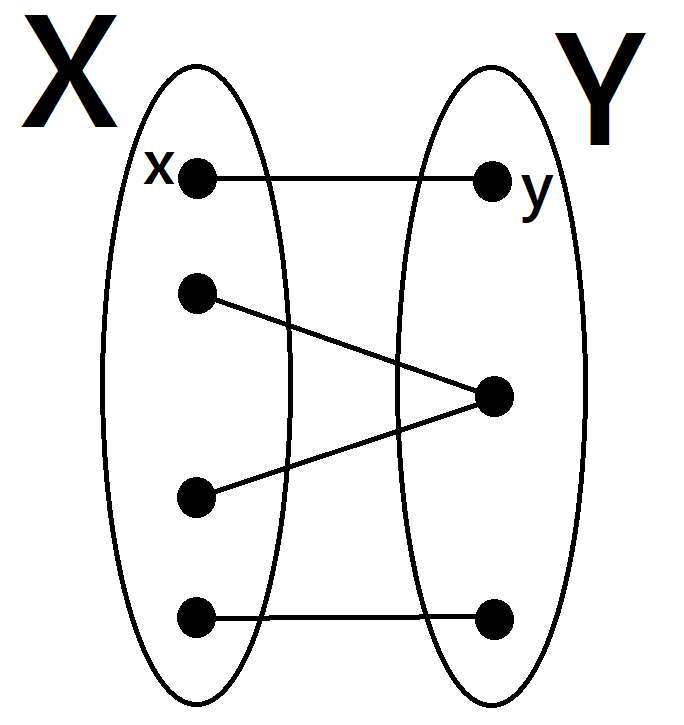
\includegraphics[width=0.2\textwidth]{img/lecture1/function}
	\end{center}
	
	\begin{definition}
		Функция $f$ называется \underline{инъекцией}, если
		\[ \forall x_1, x_2 \in X : x_1 \neq x_2 \Rightarrow f(x_1) \neq f(x_2). \]
	\end{definition}
	
	\begin{center}
		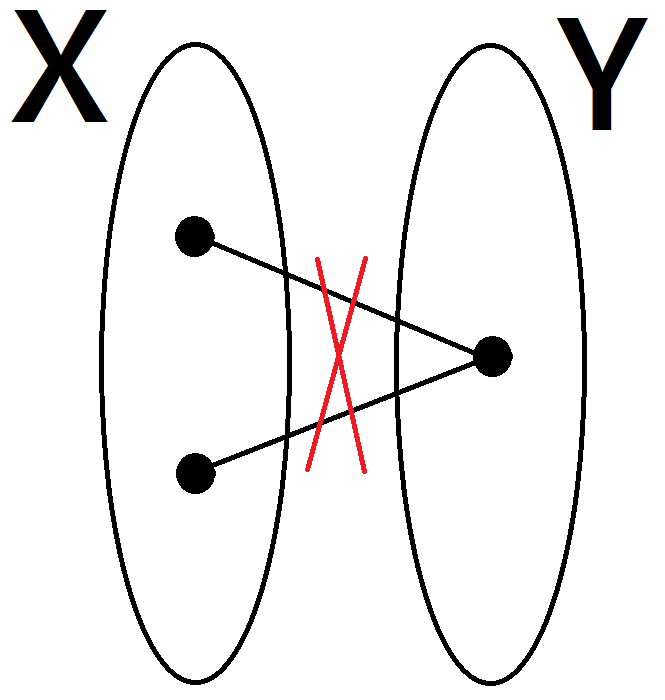
\includegraphics[width=0.2\textwidth]{img/lecture1/injection1}
		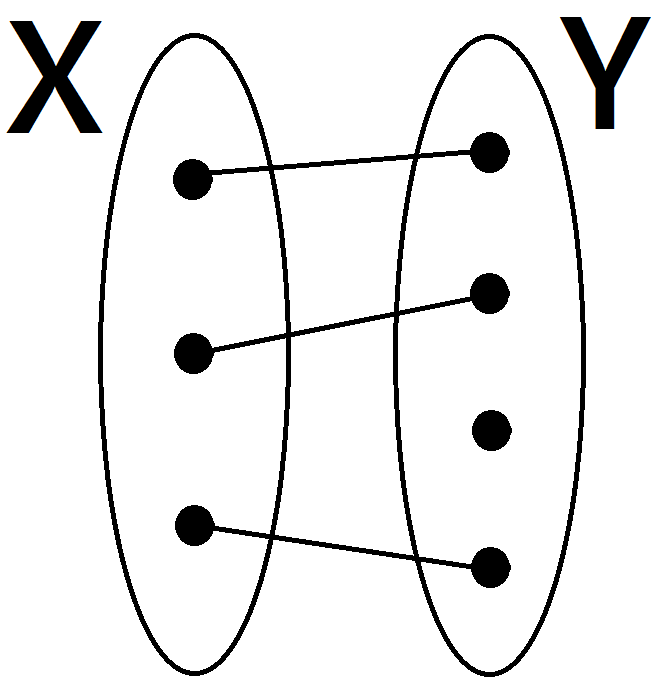
\includegraphics[width=0.2\textwidth]{img/lecture1/injection2}
	\end{center}
	
	\begin{definition}
		Функция $f$ называется \underline{сюръекцией}, если
		\[ \forall y \in Y \text{ } \exists x \in X : f(x) = y. \]
	\end{definition}
	
	\begin{center}
		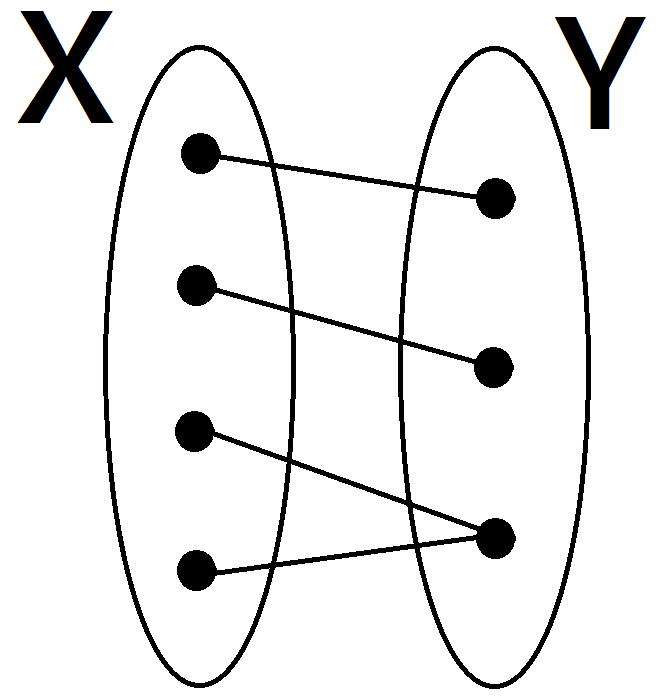
\includegraphics[width=0.2\textwidth]{img/lecture1/surjection}
	\end{center}
	
	\begin{definition}
		Функция называется \underline{биекцией}, если она одновременно является инъекцией и сюръекцией.
	\end{definition}
		
	\begin{center}
		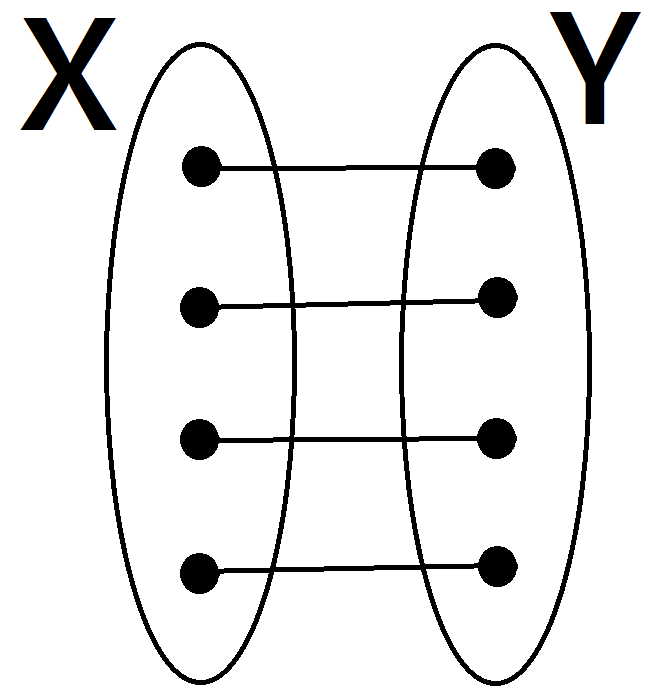
\includegraphics[width=0.2\textwidth]{img/lecture1/bijection}
	\end{center}
	
	\begin{sentence}
		Если $f$ - биекция, то существует обратная функция $f^{-1}$, для которой $f^{-1}(y) = x \Leftrightarrow f(x) = y.$
	\end{sentence}
	
	\begin{proof}
		$f$ - биекция $\Rightarrow f$ - инъекция, $x_1 \neq x_2 \Rightarrow f(x_1) \neq f(x_2)$
		
		$f$ - сюръекция $\Rightarrow \forall y$ $\exists x: f(x) = y$
		
		\begin{center}
		    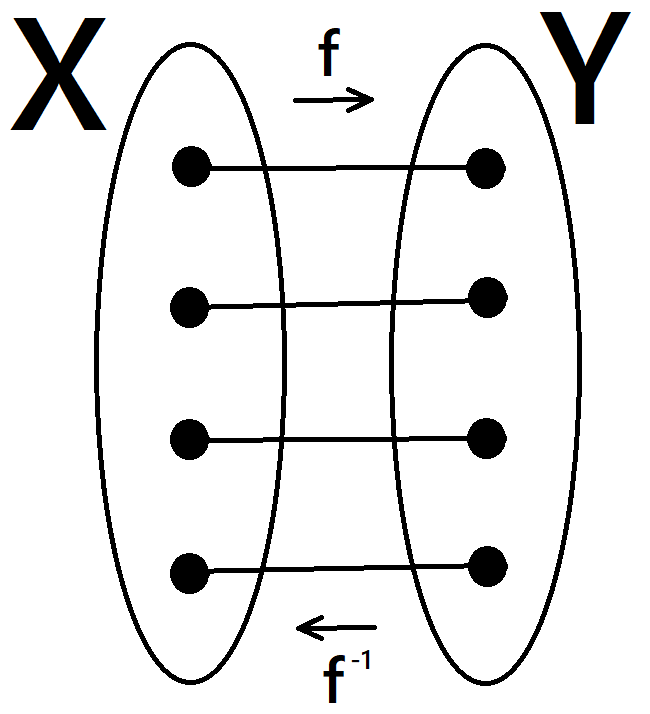
\includegraphics[width=0.3\textwidth]{img/lecture1/proof_bijection}
		\end{center}
		(Обозначение: если $f(x) = y$, то $f^{-1}(y) = x$)
		
		Определение функции для наглядности: 
		\[ \forall x \in X \text{ } \exists! y \in Y : f(x) = y \]
		\[ \forall y \in Y \text{ } \exists \text{(сюръекция)} ! \text{(инъекция)} \text{ } x \in X : f(x) = y \Leftrightarrow \forall y \in Y \text{ } \exists! x \in X : f^{-1}(y) = x. \]
	\end{proof}
	
	\section{Последовательность}
	
	\begin{definition}
		Последовательностью элементов из множества $X$ называется функция $f: \N \rightarrow X$.
	\end{definition}
	
	\begin{example}
		\begin{tabular}{|c|c|c|c|c|c|}
			\hline
			$x_1$ & $x_2$ & $x_3$ & $x_4$ & $x_5$ & ... \\
			\hline
			$2$ & $4$ & $\pi$ & $12$ & $-1$ & ... \\
			\hline
		\end{tabular}
		
		\begin{center}
			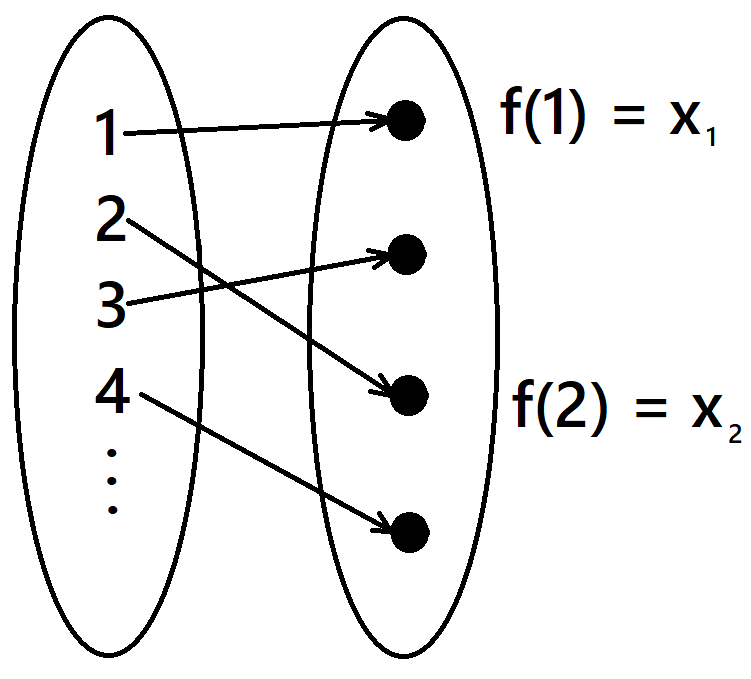
\includegraphics[width=0.3\textwidth]{img/lecture1/sequence}
		\end{center}
	\end{example}
	
	\section{Вещественные числа I: аксиомы}
	
	\begin{definition}
		Множеством действительных (вещественных) чисел $\R$ называется множество, на котором определены операции сложения и умножения и отношение порядка $\leqslant$, удовлетворяющие следующим 16 аксиомам, и которое состоит
		более чем из одного элемента.
	\end{definition}
	
	\underline{Аксиомы сложения}
	
	1. $\forall a, b \in \R \rightarrow a + b = b + a;$
	
	2. $\forall a, b, c \in \R \rightarrow (a + b) + c = a + (b + c);$
	
	3. $\exists 0 \in \R : \forall a \in \R \rightarrow a + 0 = a;$
	
	4. $\forall a \in \R$ $\exists -a \in \R : a + (-a) = 0.$
	
	\underline{Аксиомы умножения}
	
	5. $\forall a, b \in \R \rightarrow a \cdot b = b \cdot a;$
	
	6. $\forall a, b, c \in \R \rightarrow (a \cdot b) \cdot c = a \cdot (b \cdot c);$
	
	7. $\exists 1 \in \R : \forall a \in \R \rightarrow a \cdot 1 = a;$
	
	8. $\forall a \in \R \setminus \{0\}$ $\exists \frac{1}{a} \in \R : a \cdot \frac{1}{a} = 1.$
	
	\underline{Аксиома связи сложения и умножения}
	
	9. $\forall a, b, c \in \R \rightarrow a \cdot (b + c) = a \cdot b + a \cdot c.$
	
	\begin{example}
	    Докажите, что если $a, b \in \R$ и $b + a = a$, то $b = 0$.
	\end{example}
	
	\begin{proof}
		$b = 0 + b = a + (-a) + b = a + b + (-a) = a + (-a) = 0$
	\end{proof}
	
	\underline{Аксиомы отношения порядка}
	
	10. $\forall a \in \R \rightarrow a \leqslant a;$
	
	11. $\forall a, b \in \R \rightarrow a \leqslant b$ или $b \leqslant a;$
	
	12. $\forall a, b \in \R : (a \leqslant b$ и $b \leqslant a) \rightarrow a = b;$
	
	13. $\forall a, b, c \in \R : (a \leqslant b$ и $b \leqslant c) \rightarrow a \leqslant c.$
	
	\underline{Связь отношения порядка и сложения}
	
	14. $\forall a, b, c \in \R : a \leqslant b \rightarrow a + c \leqslant b + c.$
	
	\underline{Связь отношения порядка и умножения}
	
	15. $\forall a, b, c \in \R : (a \leqslant b$ и $0 \leqslant c) \rightarrow a \cdot c \leqslant b \cdot c.$
	
	Аксиомы 1-15 известны Вам из школы как свойства действительных чисел. С другой стороны, эти аксиомы определяют алгебраические структуры. В частности, аксиомы 1-4 означают, что $\R$ является абелевой (т.е. коммутативной или перестановочной) группой по сложению. Аксиомы 5-8 говорят, что $\R \setminus \{0\}$ является абелевой группой по умножению. Аксиомы 1-9 соответствуют определению поля, а аксиомы 1-15 - определению упорядоченного поля.
	
	\underline{Аксиома непрерывности}
	
	16. Если $A, B \subset \R$ и множество $A$ лежит слева от множества $B$ (т.е. $\forall a \in A$ $\forall b \in B \rightarrow a \leqslant b$), то $\exists c \in \R : \forall a \in A$ $\forall b \in B \rightarrow a \leqslant c \leqslant b.$
	
	\section{Вещественные числа II: сечения Дедекинда}
	
	Рациональные числа: $\Q = \{\frac{p}{q} \text{ } | \text{ } p \in \Z, q \in \N\}$
	
	\begin{definition}
		Дедекиндово сечение - это упорядоченная пара непустых непересекающихся подмножеств $A$ и $B$ в множестве рациональных чисел $\Q$, обладающих следующими свойствами:
		\begin{itemize}
			\item $A \cup B = \Q, A \cap B = \varnothing;$
			\item если $a \in A$ и $b \in B$, то $a < b;$
			\item в $A$ нет наибольшего элемента.
		\end{itemize}
	\end{definition}
	
	\begin{definition}
		Вещественное число — это дедекиндово сечение. Для удобства в определении будем использовать только множество $A$ (потому что, имея множество $A$, можно достроить множество $B$).
	\end{definition}
	
	\underline{Вопрос.} Чем отличаются иррациональные числа от рациональных?
	
	\underline{Ответ.} В том, что если в $B$ есть минимальный элемент, то этот минимальный элемент - это рациональное число, иначе минимальный элемент - иррациональное число, значит $B$ не имеет минимального элемента.
	
	\[ A = \{x \in \Q \text{ } | \text{ } x^2 < 2\} \cup \{x \in \Q \text{ } | \text{ } x < 0\} \]
	
	\begin{center}
		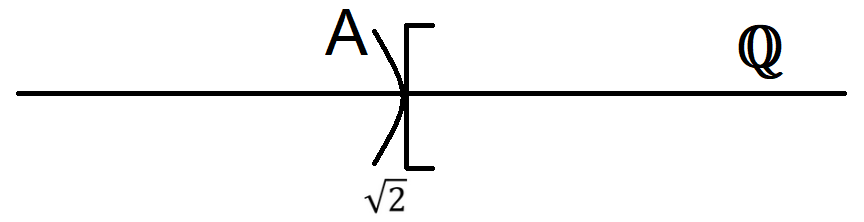
\includegraphics[width=0.6\textwidth]{img/lecture1/sqrt_of_two}
	\end{center}
	
	\begin{itemize}
		\item На множестве сечений можно определить определить арифметические операции и порядок. 
		\item Например, сложение определяется следующим образом:
	     \[ A + B := \{a + b : a \in A \wedge b  \in B\}. \]
	     \begin{center}
	     	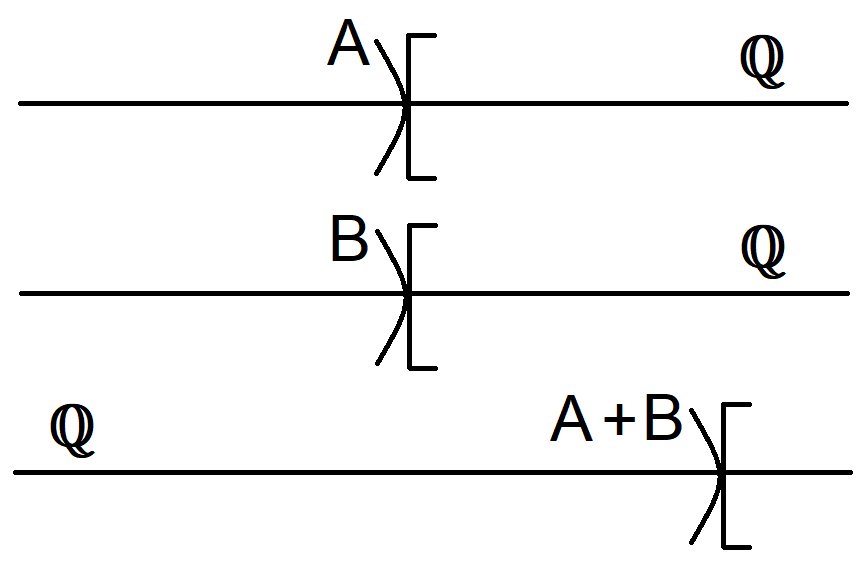
\includegraphics[width=0.4\textwidth]{img/lecture1/addition}
	     \end{center}
	    \item Умножение устроено несколько сложнее:
		\begin{itemize}
		    \item если $A, B \geqslant 0$, то
		    \[ A \times B := \{a \times b : a \geqslant 0 \wedge a \in A \wedge b  \geqslant 0 \wedge b \in B\} \cup \{x \in Q : x < 0\} \]
		    \item если $A$ или $B$ отрицательны, используем тождества 
		    \[ A \times B = -(A \times -B) = -(-A \times B) = (-A \times -B) \] чтобы преобразовать $A$ и/или $B$ в положительные числа, а затем использовать пункт выше.
		\end{itemize}
		\item Сечения Дедекинда удовлетворяют аксиомам вещественных чисел.
	\end{itemize}
	
	Проверка аксиом: \href{http://ikfia.ysn.ru/wp-content/uploads/2018/01/Landau1947ru.pdf}{Эдмунд Ландау. Основы анализа, 1947.}
	
	\section{Вещественные числа III: бесконечные десятичные последовательности}
	
	\begin{definition}
		Вещественное число можно определить как бесконечную
		десятичную дробь:
		\[ \pm a_0, a_1 a_2 ... a_n ... \]		
		где $a_0$ — целое неотрицательное число, $a_1$, $a_2$, ... $a_n$, ... - последовательность десятичных знаков.
	\end{definition}
	
	\begin{itemize}
		\item Сравнить бесконечные десятичные дроби можно поразрядно.
		\item Как сложить два вещественных числа?
	\end{itemize}
	
	\href{https://timofey.pro/static/pdfdocs/AI_004_Ter_Krikorov_2001_672s.pdf}{Тер-Крикоров А. М., Шабунин М. И. Курс математического анализа.}
	
    Последовательность из бесконечного количества 9 в этом определении запрещаем: $0,(9) = 1$.
    
    $0,(9) = x$ $| \cdot  10 \Rightarrow 9,(9) = 10x$ $| -x \Rightarrow 9 = 9x$ $| \cdot \frac{1}{9} \Rightarrow x = 1$
    
    Здесь применяем следующие аксиомы:
    
    \begin{enumerate}
    	\item $a = b \rightarrow \forall c$ $a + c = b + c$
    	\item $a = b \rightarrow \forall c$ $a \cdot c = b \cdot c$
    \end{enumerate}
	
	\begin{theorem}
		При таком определении для вещественных чисел выполнена
		аксиома непрерывности.
	\end{theorem}
	
	\newpage

	\section*{Лекция 2: Множества, функции, вещественные числа}
	
	\begin{proof}[Доказательство теоремы 1.18]
		Аксиома непрерывности:
		
		Если $A \neq \varnothing$ и $B \neq \varnothing$ таковы, что $\forall a \in A$ и $\forall b \in B \rightarrow a \leqslant b,$ то $\exists c: \forall a \in A, \forall b \in B \rightarrow a \leqslant c \leqslant b.$
		
		$b := \pm b_0, b_1 b_2 b_3 ... \in B$
		
		$\exists a \in A: \forall b \in B$ $a \leqslant b$
		
		Множество целых частей элементов из $B$ ограничено снизу. Возьмём в $B$ все числа, которые начинаются с $b_0$, ...
		
		Возьмём минимальное $b_1$ для тех $b$, которые начинаются с $b_0, ...$
		
		Возьмём минимальное $b_2$ для тех $b$, которые начинаются с $b_0, b_1 ...$
		
		$\dots$
		
		\begin{tabular}{cccccc}
			& $b_0,$ & $b_1$ & $b_2$ & ... \\
			& || & || & || &  \\
			$c =$ & $c_0,$ & $c_1$ & $c_2$ &  \\
		\end{tabular}
		
		Докажем следующие утверждения:
		\begin{enumerate}
			\item $\forall b \in B \rightarrow c \leqslant b$
			
			Пусть $\exists b \in B,$ что $b < c$
			
			\begin{center}
				\begin{tabular}{r}
					$b_0, b_1 b_2 \dots b_k b_{k + 1}$ \\
					$\wedge$ $\text{ }$ \\
					$c_0, c_1 c_2 \dots c_k c_{k + 1}$ \\
				\end{tabular}
			\end{center}
			
			Получаем противоречие, т. к. в качестве $c_{k + 1}$ мы берём минимальный $b_{k + 1}$ среди тех, которые начинаются с $b_0, b_1 b_2 ... b_k ...$
			
			\item $\forall a \in A \rightarrow c \geqslant a$
			
			\begin{center}
				\begin{tabular}{ccccccc}
					$a =$ & $a_0,$ & $a_1$ & $\dots$ & $a_k$ & $a_{k + 1}$ & $\dots$ \\
					& || & || & & || & $\vee$ & \\
					$c =$ & $c_0,$ & $c_1$ & $\dots$ & $c_k$ & $c_{k + 1}$ & $\dots$ \\
					& || & || & & || & || & \\
					$b =$ & $b_0,$ & $b_1$ & $\dots$ & $b_k$ & $b_{k + 1}$ & $\dots$ \\
				\end{tabular}
			\end{center}
			
			Тогда $b < a$ - противоречие.	
		\end{enumerate}
	\end{proof}
	
	\section{Вещественная прямая}
	
	Множество вещественных чисел также представляют в виде вещественной прямой.
	
	\begin{definition}
		\begin{itemize}
			\item интервал: $(a, b) = \{x \in \R : a < x < b\};$
			\item отрезок: $[a, b] = \{x \in \R : a \leqslant x \leqslant b\};$
			\item полуинтервалы: $[a, b) = \{x \in \R : a \leqslant x < b\}, (a, b] = \{x \in \R : a < x \leqslant b\};$
			\item лучи:
			\[ [a, +\infty) = \{x \in \R : a \leqslant x\}, (a, +\infty) = \{x \in \R : a < x\}, \]
			\[ (-\infty, a] = \{x \in \R : x \leqslant a\}, (-\infty, a) = \{x \in \R : x < a\}; \]
			\item точка: $\{a\};$
			\item числовая прямая: $(-\infty, +\infty) = \R.$
		\end{itemize}
	\end{definition}
	
	\section{Верхняя и нижняя грани}
	
	\begin{definition}	
		\begin{enumerate}
			\item Число $M \in \R$ называется верхней гранью множества $A \subset \R$, если число $M$ лежит справа от множества $A$, т. е. $\forall a \in A \rightarrow a \leqslant M.$
			\item Множество $A \subset \R$ называется ограниченным сверху, если существует (конечная) верхняя грань этого множества: $\exists M \in \R : \forall a \in A \rightarrow a \leqslant M.$
			\item Число $m \in \R$ называется нижней гранью множества $A \subset \R$, если число $m$ лежит слева от множества $A$, т. е. $\forall a \in A \rightarrow a \geqslant m.$
			\item Множество $A \subset \R$ называется ограниченным снизу, если существует (конечная) нижняя грань этого множества: $\exists m \in \R : \forall a \in A \rightarrow a \geqslant m.$
			\item Множество $A$ называется ограниченным, если $A$ ограничено сверху и ограничено снизу.
		\end{enumerate}
	\end{definition}
	
	\section{Максимальный и минимальный элементы}
	
	\begin{definition}
		Число $M$ называется максимальным элементом множества $A \subset \R$ (пишут $M = \max{A}$), если
		\begin{itemize}
			\item $M \in A,$
			\item $M$ является верхней гранью $A$.
		\end{itemize}
		Число m называется минимальным элементом множества $A \subset \R$ (пишут $m = \min{A}$), если
		\begin{itemize}
			\item $m \in A,$
			\item $m$ является нижней гранью $A$.
		\end{itemize}
	\end{definition}
	
	\section{Супремум}
	
	\begin{definition}
		Число $M \in \R$ называется точной верхней гранью или супремумом множества $A \subset \R$ (пишут: $M = \sup{A}$), если
		\begin{enumerate}
			\item $M$ является верхней гранью множества $A$ и
			\item не существует числа, меньшего, чем $M$, и являющегося верхней гранью множества $A$,
		\end{enumerate}
		то есть
		\begin{enumerate}
			\item $\forall a \in A \rightarrow a \leqslant M$ и
			\item $\neg (\exists M' \in \R : M' < M$ и $\forall a \in A \rightarrow a \leqslant M').$
		\end{enumerate}
	\end{definition}
	
	\begin{mention}
		Пункт (2) определения супремума можно записать в виде
		\[ \forall M' < M \rightarrow \neg (\forall a \in A \rightarrow a \leqslant M')\]		
		или
		\[ \forall M' < M \text{ } \exists a \in A : M' < a. \]
	\end{mention}
	
	\section{Инфимум}
	
	\begin{definition}
		Число $m \in \R$ называется точной нижней гранью или инфимумом множества $A \subset \R$ (пишут: $m = \inf{A}$), если $m$	является максимальной нижней гранью $A$.
	\end{definition}
	
	\begin{theorem}
		Пусть множество $A \subset \R$ ограничено сверху. Тогда существует
		единственное число $M \in \R$, которое является точной верхней гранью (супремум) множества $A$.
	\end{theorem}
	
	Аналогичное утверждение верно и для инфимума.
	
	\begin{proof}
		$A \subset \R$ - ограничено сверху $\Rightarrow \exists M \in \R : \forall a \in A \rightarrow a \leqslant M$.
		
		Пусть $B$ множество верхних граней $A$.
		
		Тогда $B \neq \varnothing$ $(M \in B)$.
		
		$\forall a \in A$ и $\forall b \in B \rightarrow a \leqslant b \Rightarrow$ по аксиоме непрерывности $\exists c \in \R : \forall a \in A, \forall b \in B$ $a \leqslant c \leqslant b$.
		
		Докажем, что $c = \sup{A}$.
		\begin{enumerate}
			\item $c \in B$.
			
			$\forall a \in A \rightarrow a \leqslant c \Rightarrow c \in B$
			
			\item $c$ - минимальная верхняя грань.
			
			Пусть $\exists b \in B : b < c$ - противоречит построению $c$ (аксиома непрерывности).
		\end{enumerate}
	\end{proof}
	
	\newpage
	
	\chapter{Предел последовательности}
	
	\section*{Лекция 3: Предел числовой последовательности}
	
	\section{Числовая последовательность}
	
	\begin{definition}
		Числовой последовательностью $\{a_n\}$ называется функция $a : \N \rightarrow \R$, где $a(n) = a_n$ для любого $n \in \N$. Элемент
		последовательности - это пара $(n, a_n)$, где $n$ - номер элемента
		последовательности, а $a_n$ - значение элемента последовательности.
	\end{definition}
	
	\section{Предел последовательности}
	
	\begin{definition}
		Пусть заданы числа $a, \epsilon \in \R, \epsilon > 0$. Интервал  $B_{\epsilon}(a) = (a - \epsilon, a + \epsilon)$ называется $\epsilon$-окрестностью числа $a$.
	\end{definition}
	
	\begin{definition}
		Число $a \in \R$ называется пределом последовательности $\{a_n\}$ (пишут $a = \lim_{n \to \infty} a_n$ или $a_n \to a$ при $n \to \infty$), если
		\[ \forall \epsilon > 0 \text{ } \exists N : \forall n \geqslant N \rightarrow a_n \in B_{\epsilon}(a), \]
		т. е.
		\[ \forall \epsilon > 0 \text{ } \exists N : \forall n \geqslant N \rightarrow |a_n - a| < \epsilon \]
		(здесь и далее в аналогичных выражениях, если не оговорено противное, мы подразумеваем, что $n, N$ - натуральные числа).
	\end{definition}
	
	\begin{example}
		Последовательность $a_n = \frac{1}{n}$ сходится к числу $a = 0$.
	\end{example}
	\[ \forall \epsilon > 0 \text{ } \exists N : \forall n \geqslant N \rightarrow |a_n - a| < \epsilon \]
	\[ a = 0, \text{ } |a_n - a| = \bigg|\frac{1}{n} - 0\bigg| = \frac{1}{n} < \epsilon \]
	При этом $n = \big[\frac{1}{\epsilon}\big] + 1$ неравенство выполнено
	\[ \forall \epsilon > 0 \text{ } \exists N(\epsilon) = \bigg[\frac{1}{\epsilon}\bigg] + 1 : \forall n \geqslant N(\epsilon) \text{ } |a_n - a| = \frac{1}{n} < \epsilon. \]
	
	\begin{example}
		Последовательность $a_n = (-1)^n$ не имеет предела.
	\end{example}
	От противного. Пусть
	\[ \exists a \in \R : \forall \epsilon > 0 \text{ } \exists N : \forall n \geqslant N \text{ } |a_n - a| < \epsilon \]
	Для $\epsilon = \frac{1}{2}$ $\exists N: \forall n \geqslant N$ $|a_n - a| < \frac{1}{2}$
	\[ 2 = |a_n - a_{n + 1}| = |a_n - a + a - a_{n + 1}| \leqslant |a_n - a| + |a - a_{n + 1}| (\text{неравенство треугольника}) < \]
	\[ < \frac{1}{2} + \frac{1}{2} = 1 \Rightarrow 2 < 1 - \text{противоречие}. \]
	
	\begin{mention}
		Пусть $\alpha > 0$ - фиксированное число. Тогда свойство
		\[ \forall \epsilon > 0 \text{ } \exists N(\epsilon) \in \N : \forall n > N(\epsilon) \text{ } |a_n - a| \leqslant \alpha \epsilon \]
		равносильно тому, что $\lim_{n \to \infty} a_n = a.$
	\end{mention}
	
	\begin{proof}
		\begin{itemize}
			\item[$\Leftarrow$] $\forall \epsilon' > 0$ $\exists N_1 : \forall n \geqslant N_1$ $|a_n - a| < \epsilon'$ (определение предела)
			
			$\epsilon' = \alpha \epsilon$
			
			Для $\epsilon'$ $\exists N_1: \forall n \geqslant N_1$ $|a_n - a| < \epsilon' = \alpha \epsilon$
			\item[$\Rightarrow$] $\forall \epsilon > 0$ $\exists N: \forall n \geqslant N$ $|a_n - a| \leqslant \epsilon \alpha$
			
			Пусть $\epsilon = \frac{\epsilon'}{2 \alpha}$. Тогда $|a_n - a| \leqslant \epsilon \alpha = \frac{\epsilon'}{2 \alpha} \cdot \alpha = \frac{\epsilon'}{2}$.
			
			\[ \forall \epsilon' > 0 \text{ } \exists N_1 = N\bigg(\frac{\epsilon'}{2 \alpha}\bigg) + 1: \forall n > N_1 \text{ } |a_n - a| \leqslant \frac{\epsilon'}{2} < \epsilon' \]
		\end{itemize}
	\end{proof}
	
	\section{Единственность предела}
	
	\begin{sentence}
		Пусть $\lim_{n \to \infty} a_n = a$ и $\lim_{n \to \infty} a_n = b$, тогда $a = b$.
	\end{sentence}
	
	\begin{proof}
		\begin{enumerate}
			\item $\forall \epsilon > 0$ $\exists N_1: \forall n \geqslant N_1$ $|a_n - a| < \epsilon$
			\item $\forall \epsilon > 0$ $\exists N_2: \forall n \geqslant N_2$ $|a_n - b| < \epsilon$
		\end{enumerate}
		Пусть $a \neq b, |a - b| = \epsilon_0 > 0$.
		
		Возьмём такие $N_1$ и $N_2$, что $|a_n - a| < \frac{\epsilon_0}{2}$ и $|a_n - b| < \frac{\epsilon_0}{2}$.
		
		Тогда $\forall n \geqslant \max{(N_1, N_2)}$
		\[ \epsilon_0 = |a - b| = |a - a_n + a_n - b| \leqslant |a - a_n| + |a_n - b| < \frac{\epsilon_0}{2} + \frac{\epsilon_0}{2} = \epsilon_0 \Rightarrow \epsilon_0 < \epsilon_0 - \]
		противоречие.
	\end{proof}
	
	\section{Ограниченная последовательность}
	
	\begin{definition}
		Последовательность $\{a_n\}^{\infty}_{n = 1}$ называется \textbf{ограниченной}, если существуют такие числа $C, c \in \R,$ что $c \leqslant a_n \leqslant C$ для каждого $n \in \N$.
	\end{definition}
	
	\begin{mention}
		\begin{enumerate}
			\item Последовательность ограничена сверху, если
			
			$\exists C : \forall n$ $a_n \leqslant C$.
			\item Последовательность ограничена снизу, если $\exists c : \forall n$ $a_n \geqslant c$.
		\end{enumerate}
	\end{mention}
	
	\begin{sentence}
		Сходящаяся последовательность ограничена.
	\end{sentence}
	
	\begin{proof}
		Пусть есть последовательность $\{a_n\}^{\infty}_{n = 1}, \lim_{n \to \infty} a_n = a$.
		
		$\forall \epsilon > 0$ $\exists N: \forall n \geqslant N$ $|a_n - a| < \epsilon$
		
		$\exists N: \forall n \geqslant N$ $|a_n - a| < 1 \Rightarrow$ по неравенству треугольника $|a_n| - |a| \leqslant |a_n - a| < 1 \Rightarrow |a_n| < |a| + 1$
		
		$\forall n$ $|a_n| \leqslant \max\{|a_1|, |a_2|, ..., |a_N|, |a| + 1\} \Rightarrow \forall n$ $c \leqslant a_n \leqslant C,$ где
		
		$c = -\max\{|a_1|, |a_2|, ..., |a_N|, |a| + 1\}, C = \max\{|a_1|, |a_2|, ..., |a_N|, |a| + 1\}.$
	\end{proof}
	
	\begin{lemma}[Об отделимости]
		Если $a_n \rightarrow a$ и $a \neq 0$, то найдется номер $N \in \N$, для которого $|a_n| > \frac{|a|}{2} > 0$ при $n > N$.
	\end{lemma}
	
	\begin{proof}
		$a_n \to a \Rightarrow \forall \epsilon > 0$ $\exists N: \forall n > N$ $|a_n - a| < \epsilon$
		
		$\epsilon = \frac{|a|}{2} > 0$ $\exists N: \forall n \geqslant N$ $|a_n - a| < \frac{|a|}{2}$
		
		Тогда по неравенству треугольника $|a| - |a_n| \leqslant |a_n - a| < \frac{|a|}{2} \Rightarrow |a_n| > \frac{|a|}{2}.$
	\end{proof}
	
	\section{Арифметические свойства предела}
	
	\begin{theorem}
		Пусть $\lim_{n \to \infty} a_n = a$ и $\lim_{n \to \infty} b_n = b$. Тогда
		\begin{enumerate}
			\item $\lim_{n \to \infty} (\alpha a_n + \beta b_n) = \alpha a + \beta b$ $\forall \alpha, \beta \in \R;$
			\item $\lim_{n \to \infty} a_n b_n = ab;$
			\item если $b \neq 0, b_n \neq 0$, то $\lim_{n \to \infty} \frac{a_n}{b_n} = \frac{a}{b};$
		\end{enumerate} 
	\end{theorem}
	
	\begin{proof}
		\begin{enumerate}
			\item $\forall \epsilon > 0$ $\exists N_1: \forall n \geqslant N_1$ $|a_n - a| < \epsilon$
			
			$\forall \epsilon > 0$ $\exists N_2: \forall n \geqslant N_2$ $|b_n - b| < \epsilon$
			
			$N_3 = \max\{N_1, N_2\}.$ Тогда $\forall n \geqslant N_3$ $|\alpha a_n + \beta b_n - \alpha a - \beta b| = |\alpha a_n - \alpha a + \beta b_n - \beta b| \leqslant |\alpha a_n - \alpha a| + |\beta b_n - \beta b| = |\alpha| |a_n - a| + |\beta| |b_n - b| \leqslant (|\alpha| + |\beta|)\epsilon$
			\item $\forall \epsilon > 0$ $\exists N_1: \forall n \geqslant N_1 \rightarrow |a_n - a| < \epsilon$
			
			$\forall \epsilon > 0$ $\exists N_2: \forall n \geqslant N_2 \rightarrow |b_n - b| < \epsilon$
			
			$c_n = a_n b_n$
			
			$a_1, a_2, a_3, ...$
			
			$b_1, b_2, b_3, ...$
			
			$c_1 = a_1 b_1, c_2 = a_2 b_2, c_3 = a_3 b_3, ...$
			
			Требуется доказать: $\forall \epsilon > 0$ $\exists N: \forall n \geqslant N \rightarrow |c_n - ab| = |a_n b_n - ab| < \epsilon.$
			
			$a_n$ сходится $\Rightarrow$ по предложению 2.10 $\exists C > 0: |a_n| \leqslant C.$
			
			$|a_n b_n - ab| = |a_n b_n - a_n b + a_n b - ab| \leqslant |a_n b_n - a_n b| + |a_n b - ab| = |a_n| |b_n - b| + |b| |a_n - a| \Rightarrow$ для $N = \max\{N_1, N_2\}$ $\forall n \geqslant N \rightarrow |a_n b_n - ab| \leqslant |a_n| |b_n - b| + |b| |a_n - a| < C \epsilon + |b| \epsilon = (C + |b|) \epsilon = \alpha \epsilon$ $(\alpha = C + |b| > 0)$
			
			По замечению 2.6
			\[ \forall \epsilon > 0 \text{ } \exists N = \max\{N_1, N_2\}: \forall n > N \text{ } |a_n b_n - ab| < (C + |b|) \epsilon = \alpha \epsilon. \]
			\item $\forall \epsilon > 0$ $\exists N_1: \forall n \geqslant N_1 \rightarrow |a_n - a| < \epsilon$ (1)
			
			$\forall \epsilon > 0$ $\exists N_2: \forall n \geqslant N_2 \rightarrow |b_n - b| < \epsilon$ (2)
			
			Требуется доказать: $\lim_{n \to \infty} \frac{a_n}{b_n} = \frac{a}{b}$.
			
			Докажем, что $\lim_{n \to \infty} \frac{1}{b_n} = \frac{1}{b}.$ Тогда из пункта 2 будет следовать пункт 3.
			
			$\forall \epsilon > 0$ $\exists N: \forall n \geqslant N \rightarrow \big|\frac{1}{b_n} - \frac{1}{b}\big| < \epsilon$ - требуется доказать.
			
			Оценим $\big|\frac{1}{b_n} - \frac{1}{b}\big| = \big|\frac{b - b_n}{b_n b}\big|$
			
			Из леммы 2.10 следует, что $\exists N_3: \forall n > N_3$ $|b_n| > \frac{|b|}{2} > 0$ (3)
			
			Из (1), (2) и (3) следует, что $\forall n \geqslant N_4 = \max\{N_1. N_2, N_3\}$ $\big|\frac{b - b_n}{b_n \cdot b}\big| < \frac{\epsilon}{\frac{|b|}{2} \cdot |b|} = \frac{2 \epsilon}{|b|^2} = \alpha \epsilon,$ где $\alpha = \frac{2}{|b|^2}.$ 
		\end{enumerate}
	\end{proof}
	
	\newpage
	
	\section*{Лекция 4: Теорема Вейерштрасса, число e}
	
	\begin{theorem}[Переход к пределу в неравенстве]
		Пусть $\lim_{n \to \infty} a_n = a, \lim_{n \to \infty} b_n = b$. Если для некоторого номера $N$ выполнено $a_n \leqslant b_n$ при $n > N$, то $a \leqslant b$.
	\end{theorem}
	
	\begin{proof}
		Пусть $a > b \Rightarrow a - b = \epsilon_0 > 0$
		
		$\lim_{n \to \infty} a_n = a \Rightarrow \forall \epsilon = \frac{\epsilon_0}{2}$ $\exists N_1: \forall n \geqslant N_1$ $|a_n - a| < \frac{\epsilon_0}{2}$
		
		$\lim_{n \to \infty} b_n = b \Rightarrow \forall \epsilon = \frac{\epsilon_0}{2}$ $\exists N_2: \forall n \geqslant N_2$ $|b_n - b| < \frac{\epsilon_0}{2}$
		
		$\forall n > \max\{N, N_1, N_2\}$ $\epsilon_0 = a - b = a - a_n + a_n - b_n + b_n - b \leqslant$
		
		$\leqslant \underbrace{|a - a_n|}_{< \frac{\epsilon_0}{2}} + \underbrace{a_n - b_n}_{\leqslant 0 \text{ (из условия)}} + \underbrace{|b_n - b|}_{< \frac{\epsilon_0}{2}} < \epsilon_0$
		
		$\epsilon_0 < \epsilon_0$ - противоречие.
	\end{proof}
	
	\section{Лемма о зажатой последовательности}
	
	\begin{lemma}[О зажатой последовательности]
		Пусть $\lim_{n \to \infty} a_n = \lim_{n \to \infty} b_n = a$ и для некоторого $N \in \N$ выполнено $a_n \leqslant c_n \leqslant b_n$ при $n > N$. Тогда $\lim_{n \to \infty} c_n = a$.
	\end{lemma}
	
	\begin{proof}
		Выполнено:
		\begin{enumerate}
			\item $\forall \epsilon > 0$ $\exists N_1: \forall n \geqslant N_1$ $|a_n - a| < \epsilon$ $(\Leftrightarrow a - \epsilon < a_n < a + \epsilon)$
			\item $\forall \epsilon > 0$ $\exists N_2: \forall n \geqslant N_2$ $|b_n - a| < \epsilon$ $(\Leftrightarrow a - \epsilon < b_n < a + \epsilon)$
			\item $\forall n > N$ $a_n \leqslant c_n \leqslant b_n$
		\end{enumerate}
		Из этих пунктов следует, что $\forall n \geqslant N_4 = \max{(N, N_1, N_2)}$ $\Rightarrow a - \epsilon < a_n \leqslant c_n \leqslant b_n < a + \epsilon \Rightarrow \forall n \geqslant N_4$ $a - \epsilon < c_n < a + \epsilon \Leftrightarrow |c_n - a| < \epsilon$ (это определение предела)
	\end{proof}
	
	\section{Теорема Вейерштрасса}
	
	\begin{theorem}[Вейерштрасс]
		Пусть последовательность $\{a_n\}^{\infty}_{n = 1}$ не убывает $(a_n \leqslant a_{n + 1})$ и ограничена сверху. Тогда эта последовательность сходится $x$ своему супремуму.
		
		Аналогично, пусть последовательность $\{a_n\}^{\infty}_{n = 1}$ не возрастает $(a_{n + 1} \leqslant a_n)$ и ограничена снизу. Тогда эта последовательность сходится к своему инфимуму.
	\end{theorem}
	
	\begin{proof}
		$M = \sup\{a_n | n \in \N\}$ (супремум существует, т. к. $a_n$ ограничена сверху)
		
		Пусть $\epsilon > 0$ - произвольное. Хотим доказать, что $\forall \epsilon > 0$ $\exists N: \forall n \geqslant N \rightarrow |a_n - M| < \epsilon.$
		
		$M' = M - \epsilon.$ Т. к. $M = \sup\{a_n | n \in \N\},$ то из свойства супремума ($\forall M' < M$ $\exists a \in A$ $a > M'$) следует, что  $\exists a \in \{a_n | n \in \N\}: a > M'.$
		
		Но если $a \in \{a_n | n \in \N\},$ то $\exists N: a = a_N.$ Т. е. $\exists N: a_N > M' = M - \epsilon.$
		
		Т. к. $a_n$ не убывает (т. е. $a_N \leqslant a_{N + 1}$) $\forall n \geqslant N$ $a_n \geqslant a_N > M' = M - \epsilon$ (*)
		
		Только что доказано, что $M - \epsilon < a_n$, и из-за того, что $M$ - супремум, верно $a_n < M + \epsilon$. Тогда $M - \epsilon < a_n < M + \epsilon \Leftrightarrow |a_n - M| < \epsilon.$
		
		(*) $\Rightarrow \forall \epsilon > 0$ $\exists N: \forall n \geqslant N$ $|a_n - M| < \epsilon.$
		
		Для доказательства второго утверждения можно рассмотреть последовательность $a_n \rightsquigarrow -a_n.$ Если $a_n$ не возрастает, то $-a_n$ не убывает. Последовательность $-a_n \to \sup\{-a_n | n \in \N\} \Rightarrow$ последовательность $a_n \to -\sup\{-a_n | n \in \N\} = \inf\{a_n | n \in \N\}.$
	\end{proof}
	
	\begin{example}
		Пусть $a_{n + 1} = \frac{1}{2} \big(a_n + \frac{2}{a_n}\big), a_1 = 2$. Тогда последовательность $\{a_n\}^{\infty}_{n = 1}$ сходится и её предел равен $\sqrt{2}$.
	\end{example}
	
	\begin{proof}
		\begin{enumerate}
			\item $a_n$ - ограничена снизу.
			
			Действительно, $a_{n + 1} = \frac{1}{2}\big(a_n + \frac{2}{a_n}\big) \geqslant \sqrt{a_n \cdot \frac{2}{a_n}} (\text{неравенство Коши}) = \sqrt{2} \Rightarrow a_n \geqslant \sqrt{2}.$
			
			\item $a_n$ - не возрастает
			
			$a_{n + 1} = \frac{1}{2}\big(a_n + \frac{2}{a_n}\big) = \frac{1}{2}\big(a_n + \frac{\sqrt{2} \cdot \sqrt{2}}{a_n}\big) \leqslant \frac{1}{2}\big(a_n + \frac{a_n^2}{a_n}\big) = \frac{1}{2}(a_n + a_n) = a_n \Rightarrow$ по теореме Вейерштрасса $\exists \lim_{n \to \infty} a_n = a.$
			
			$a_{n + 1} = \frac{1}{2}\big(a_n + \frac{2}{a_n}\big) \Rightarrow a = \lim_{n \to \infty} a_{n + 1} = \lim_{n \to \infty} \frac{1}{2}\big(a_n + \frac{2}{a_n}\big) = \lim_{n \to \infty} \frac{1}{2}a_n + \lim_{n \to \infty} \frac{1}{a_n} = \frac{1}{2}a + \frac{1}{a}$
			
			$a = \frac{1}{2}a + \frac{1}{a} \Rightarrow a^2 - \frac{1}{2}a^2 - 1 = 0 \Rightarrow \frac{1}{2}a^2 = 1 \Rightarrow a = \pm \sqrt{2}$
			
			$a = -\sqrt{2}$ - не подходит (поскольку $\forall n$ $a_n \geqslant \sqrt{2} > -\sqrt{2}$) $\Rightarrow a = \sqrt{2}.$
			
		\end{enumerate}
	\end{proof}
	
	\newpage
	
	\section*{Лекция 5: Число e, частичный предел}
	
	\section{Число e}
	
	\begin{sentence}
		Последовательность $a_n = \big(1 + \frac{1}{n}\big)^n$ сходится.
	\end{sentence}
	
	\begin{proof}
		\[ (a + b)^n = \sum_{k = 0}^n C_n^k a^k b^{n - k} - \text{бином Ньютона.} \]
		\[ C_n^k = \frac{n!}{k!(n - k)!} = \frac{n(n - 1)(n - 2)...(n - k + 1)}{k!} \]
		\[ a_n = \bigg(1 + \frac{1}{n}\bigg)^n = \sum_{k = 0}^n C_n^k \frac{1}{n^k} = 1 + 1 + \sum_{k = 2}^n C_n^k \frac{1}{n^k} = 2 + \sum_{k = 2}^n \frac{n(n - 1)...(n - k + 1)}{k! \underbrace{n n ... n}_{k \text{ раз}}} = \]
		\[ = 2 + \sum_{k = 2}^n \frac{1}{k!} \cdot \bigg(1 - \frac{1}{n}\bigg)\bigg(1 - \frac{2}{n}\bigg)...\bigg(1 - \frac{k - 1}{n}\bigg) \leqslant 2 + \sum_{k = 2}^n \frac{1}{k!} \leqslant (*) \]
		
		Воспользуемся неравенством: при $k \geqslant 2$ $k! = 1 \cdot 2 \cdot 3 \cdot ... \cdot k \geqslant 2^{k - 1}.$
		
		\[ (*) \leqslant 2 + \sum_{k = 2}^n \frac{1}{2^{k - 1}} \leqslant 2 + 1 = 3, \]
		значит $a_n$ ограничена, $a_n \leqslant 3.$
		
		Докажем, что $\sum_{k = 2}^n \frac{1}{2^{k - 1}} < 1$.
		
		Воспользуемся формулой суммы геометрической прогрессии.
		\[ 1 + q + q^2 + ... + q^{k - 1} = \frac{1 - q^k}{1 - q} \]
		\[ 1 + \frac{1}{2} + \frac{1}{4} + ... + \frac{1}{2^{k - 1}} = \frac{1 - \big(\frac{1}{2}\big)^k}{1 - \frac{1}{2}} = 2 \bigg(1 - \bigg(\frac{1}{2}\bigg)^k\bigg) < 2 \]
		\[ a_n = 2 + \sum_{k = 2}^n \frac{1}{k!} \bigg(1 - \frac{1}{n}\bigg)\bigg(1 - \frac{2}{n}\bigg)...\bigg(1 - \frac{k - 1}{n}\bigg) \leqslant 2 + \sum_{k = 2}^n \frac{1}{k!} \bigg(1 - \frac{1}{n + 1}\bigg)\bigg(1 - \frac{2}{n + 1}\bigg)... \]
		\[ ...\bigg(1 - \frac{k - 1}{n + 1}\bigg) < 2 + \sum_{k = 2}^{n + 1} \frac{1}{k!} \bigg(1 - \frac{1}{n + 1}\bigg)\bigg(1 - \frac{2}{n + 1}\bigg)...\bigg(1 - \frac{k - 1}{n + 1}\bigg) = a_{n + 1} \Rightarrow \]
		$\Rightarrow a_n < a_{n + 1} \Rightarrow a_n \text{ возрастает}.$
		
		По теореме Вейерштрасса $a_n$ имеет предел.
	\end{proof}
	
	\begin{definition}
		Предел последовательности $a_n = \big(1 + \frac{1}{n}\big)^n$ называют \textbf{числом Эйлера} и обозначают
		\[ \lim_{n \to \infty} \bigg(1 + \frac{1}{n}\bigg)^n = e \approx 2,71828182845904523536... \]
	\end{definition}
	
	\section{Принцип вложенных отрезков}
	
	\begin{theorem}[Принцип вложенных отрезков]
		\begin{enumerate}
			\item Всякая последовательность $\{[a_n, b_n]\}^{\infty}_{n = 1}$ вложенных отрезков (т. е. $[a_{n + 1}, b_{n + 1}] \subset [a_n, b_n]$) имеет общую точку.
			\item Кроме того, если длины отрезков стремятся к нулю, т.е. $b_n - a_n \to 0$, то такая общая точка только одна.
		\end{enumerate}
		
		\begin{center}
			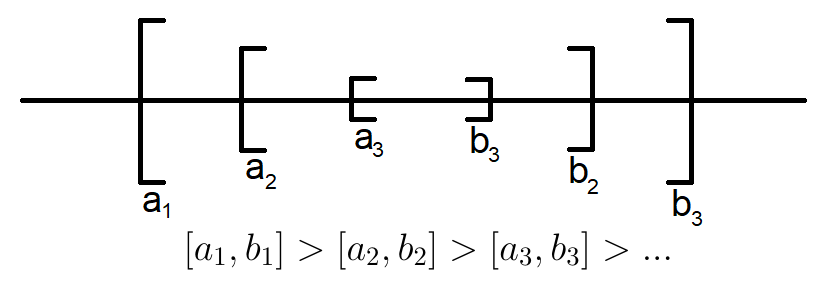
\includegraphics[width=0.5\textwidth]{img/lecture5/nested_segments}
		\end{center}
	\end{theorem}
	
	\begin{proof}
		\begin{enumerate}
			\item $\{a_n | n \in \N\} = A, \{b_n | n \in \N\} = B$
			
			$\forall n$ $a_n \leqslant b_n$
			
			$\forall n, m$ $a_n \leqslant b_m$ - докажем это.
			
			\begin{enumerate}
				\item $n > m$ $a_m \leqslant a_n \leqslant b_n \leqslant b_m$
				\item $n \leqslant m$ $a_n \leqslant a_m \leqslant b_m \leqslant b_n$
			\end{enumerate}
			Тогда $\forall a \in A$ $\forall b \in B \rightarrow a \leqslant b$
			
			Множества $A$ и $B$ непустые $\Rightarrow$ по аксиоме непрерывности $\exists c: \forall a \in A, \forall b \in B$ $a \leqslant c \leqslant b.$
			
			$\forall n \in \N$ $a_n \leqslant c \leqslant b_n$ - точка $c$ принадлежит всем отрезкам.
			
			\item Пусть $\lim_{n \to \infty} (b_n - a_n) = 0.$
			
			$\exists c_1, c_2 \in [a_n, b_n]$ - от противного $(c_1 \neq c_2)$
			
			Пусть $c_1 < c_2$ $[c_1, c_2] \subseteq [a_n, b_n].$
			
			Но тогда $b_n - a_n \geqslant c_2 - c_1 = \epsilon_0 > 0.$
			
			$b_n - a_n \to 0 \Rightarrow 0 \geqslant \epsilon_0 > 0$ - противоречие.
		\end{enumerate}
	\end{proof}
	
	\section{Подпоследовательность}
	
	\begin{theorem}
		Пусть задана последовательность $\{a_n\}^{\infty}_{n = 1}$ и пусть задана
		возрастающая последовательность натуральных чисел $n_1 < n_2 < n_3 < ...$ Последовательность $b_k = a_{n_k}$ называется \textbf{подпоследовательностью} последовательности $\{a_n\}^{\infty}_{n = 1}$. Число $a \in \R$ называется \textbf{частичным пределом} последовательности $\{a_n\}^{\infty}_{n = 1}$, если выполнено $a = \lim_{k \to \infty} a_{n_k}$ для некоторой подпоследовательности $\{a_{n_k}\}^{\infty}_{k = 1}$.
	\end{theorem}
	
	\begin{mention}
		Последовательность $a_n = (-1)^n$ не имеет предела, но его подпоследовательность $b_k = a_{2n}$ имеет предел: $\lim_{k \to \infty} b_k = 1$.
	\end{mention}
	
	\begin{sentence}
		Любая подпоследовательность сходящейся последовательности сходится к пределу этой последовательности.
	\end{sentence}
	
	\begin{proof}
		$a_n \to a$ при $n \to \infty$
		
		$\forall \epsilon > 0$ $\exists N_1: \forall n \geqslant N_1$ $|a_n - a| < \epsilon$
		
		$b_k = a_{n_k}$ $k \leqslant n_k$
		
		$\forall \epsilon > 0$ $\exists N = N_1$ $\forall k \geqslant N_1 \text{ (пояснение: } n_k \geqslant k \geqslant N_1)$ $|b_k - a| = |a_{n_k} - a| \leqslant \text{(последовательность сходится) } |a_k - a| < \epsilon.$
	\end{proof}
	
	\section{Нижний и верхний частичные пределы}
	
	\begin{definition}
		Рассмотрим последовательности $M_n := \sup_{k > n} a_k$ и $m_n := \inf_{k > n} a_k$. Ясно, что последовательность $M_n$ - не возрастает, а
		последовательность $m_n$ - не убывает. Поэтому для \textbf{ограниченной} последовательности $\{a_n\}^{\infty}_{n = 1}$ существуют пределы
		\[ \uplim_{n \to \infty} a_n := \lim_{n \to \infty} M_n, \lowlim_{n \to \infty}	a_n := \lim_{n \to \infty} m_n, \]
		которые называются соответственно \textbf{верхним и нижним частичными пределами} последовательности $\{a_n\}^{\infty}_{n = 1}$.
	\end{definition}
	
	Иллюстрация для значений $m_n$ и $M_n$.
	\begin{center}
		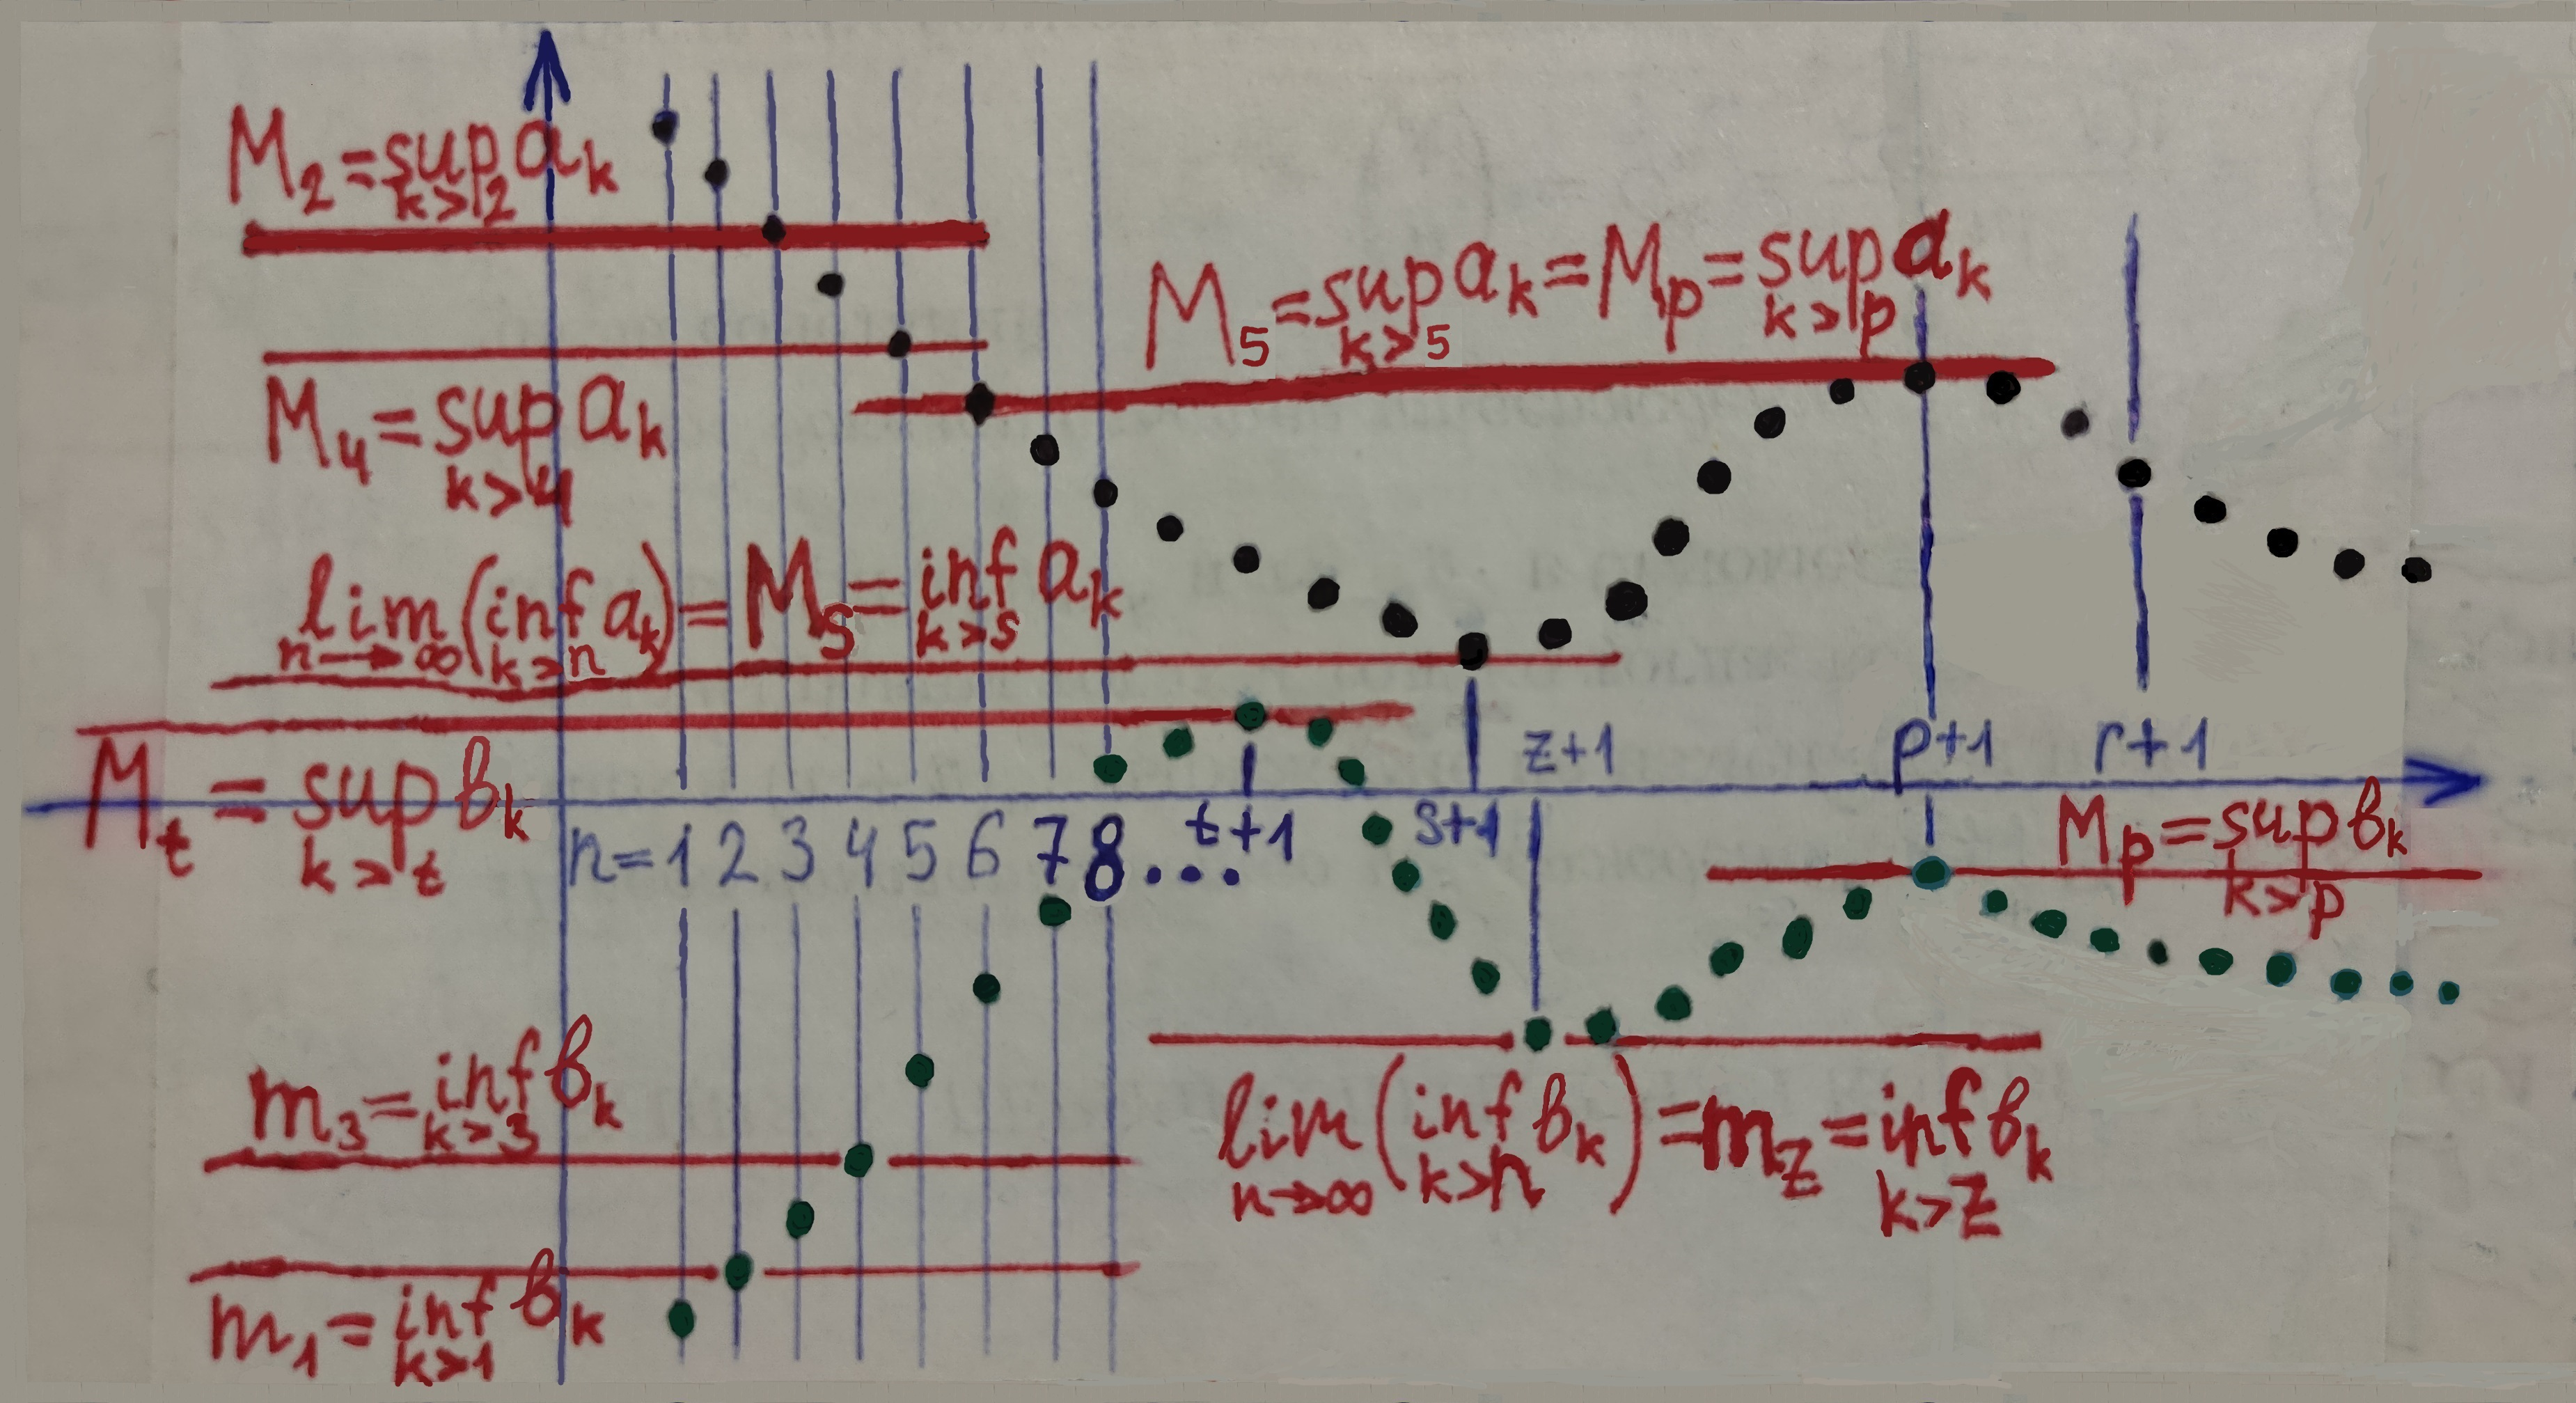
\includegraphics[width=0.7\textwidth]{img/lecture5/inf_and_sup_examples}
	\end{center}
	
	\section{Теорема Больцано}
	
	\begin{theorem}
		Пусть $\{a_n\}^{\infty}_{n = 1}$ - \textbf{ограниченная} последовательность. Тогда $\displaystyle \uplim_{n \to \infty} a_n$ и $\displaystyle \lowlim_{n \to \infty} a_n$ - частичные пределы последовательности $\{a_n\}^{\infty}_{n = 1}$ и любой другой частичный предел принадлежит отрезку $\displaystyle \bigg[\lowlim_{n \to \infty} a_n, \uplim_{n \to \infty} a_n\bigg]$.
	\end{theorem}
	
	\begin{proof}
		Пусть $\displaystyle \uplim_{n \to \infty} a_n = \lim_{n \to \infty} M_n = M.$
		
		$M_n = \sup_{k > n} a_k$
		
		Построим последовательность $a_{n_k}$, которая обладает свойством $\lim_{k \to \infty} a_{n_k} = M$. Пусть $n_1 = 1.$ Пусть построены первые $j$ членов (т. е. подобраны $n_1 < n_2 < ... < n_j$). Подберём $n_{j + 1}$-й номер ($n_{j + 1} > n_{j}$).
		
		$M_{n_j} = \sup_{k > n_j} a_k$
		
		\begin{center}
			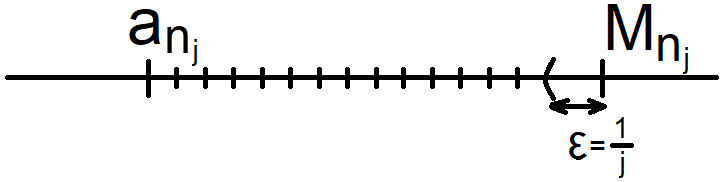
\includegraphics[width=0.5\textwidth]{img/lecture5/theorem_bolcano}
		\end{center}
		
		Т. к. $M_{n_j}$ - супремум, то $\exists a \in \{a_k | k > n_j\}$ такое, что
		$M_{n_j} - \frac{1}{j} \leqslant a \leqslant M_{n_j}$ (в противном случае $M_{n_j}$ - не супремум). Т. к. $a \in \{a_k | k > n_j\},$ то пусть $a = a_{\lambda}$ $n_j > n_{j + 1} = \lambda.$
		
		$\forall j \in \N$ $M_{n_j} - \frac{1}{j} \leqslant a_{n_{j + 1}} \leqslant M_{n_j}$ . Т. к. $M_j \to M, \frac{1}{j} \to 0,$ то по теореме о зажатой последовательности
		\[ M - 0 \leqslant \lim_{j \to \infty} a_{n_{j + 1}} \leqslant \lim_{j \to \infty} M_{n_j} = \text{(предложение 2.13) } M \]
		Значит $\lim_{j \to \infty} a_{n_j} = M \Rightarrow \uplim_{n \to \infty} a_n$ - частичный предел.
		
		Теперь пусть $\lowlim_{n \to \infty} a_n = \lim_{n \to \infty} m_n = m.$
		
		Аналогично можно доказать, что
		\[ \forall j \in \N \text{ } m_{n_j} \leqslant a_{n_{j + 1}} \leqslant m_{n_j} + \frac{1}{j} \]
		\[ m = \lim_{j \to \infty} m_{n_j} \leqslant \lim_{j \to \infty} a_{n_{j + 1}} \leqslant m + 0 \]
		$\lim_{j \to \infty} a_{n_{j + 1}} = m \Rightarrow \lowlim_{n \to \infty} a_n$ - частичный предел.
		
		Пусть теперь $a$ - частичный предел. Это означает, что $a = \lim_{k \to \infty} a_{n_k}$ для некоторой подпоследовательности $\{a_{n_k}\}^{\infty}_{k = 1}.$ Тогда $\displaystyle \inf_{p > n_{k - 1}} a_p = m_{n_{k - 1}} \leqslant a_{n_k} \leqslant M_{n_{k - 1}} = \sup_{p > n_{k - 1}} a_p.$ По теореме о переходе к пределу в неравенстве получаем, что $\displaystyle \lowlim_{n \to \infty} a_n \leqslant a \leqslant \uplim_{n \to \infty} a_n.$
	\end{proof}
	
	\begin{corollary}[Теорема Больцано]
		Во всякой \textbf{ограниченной} последовательности можно найти сходящуюся подпоследовательность.
	\end{corollary}
	
	Можно, потому что, например, есть верхний частичный предел, который является частичным пределом соответствующей последовательности.
	
	\newpage
	
	\section*{Лекция 6: Критерий Коши}
	
	\begin{theorem}
		\textbf{Ограниченная} последовательность сходится тогда и только тогда, когда множество её частичных пределов состоит из одного элемента.
	\end{theorem}
	
	\begin{proof}
		\begin{itemize}
			\item[$\Rightarrow$] предложение 2.22
			\item[$\Leftarrow$] Т. к. множество частичных пределов состоит из одного элемента, то
			\[ \lowlim_{n \to \infty} a_n = \uplim_{n \to \infty} a_n = a \]
			\[ \lowlim_{n \to \infty} a_n = \lim_{n \to \infty} m_n, m_n = \inf_{k > n} \{a_k\}, \uplim_{n \to \infty} a_n = \lim_{n \to \infty} M_n, M_n = \sup_{k > n} \{a_k\} \]
			Тогда $\forall n$ $m_{n - 1} \leqslant a_n \leqslant M_{n - 1}.$
			
			Т. к. $m_{n - 1} \to a, M_{n - 1} \to a,$ то по теореме о зажатой последовательности $\lim_{n \to \infty} a_n = a.$
		\end{itemize}
	\end{proof}
	
	\section{Фундаментальная последовательность}
	
	\begin{definition}
		Говорят, что последовательность $\{a_n\}^{\infty}_{n = 1}$ \textbf{фундаментальна} (или является последовательностью Коши), если для каждого числа $\epsilon > 0$ найдется такое натуральное число (номер) $N(\epsilon) \in \N$, что $|a_n - a_m| < \epsilon$ при каждых $n, m > N(\epsilon).$ То же
		самое утверждение можно переписать в кванторах следующим образом:
		\[ \forall \epsilon > 0 \text{ } \exists N(\epsilon) \in \N : \forall n, m > N(\epsilon) \text{ } |a_n - a_m| < \epsilon. \]
	\end{definition}
	
	\begin{example}
		\begin{enumerate}
			\item Последовательность $a_n = \frac{1}{n}$ - фундаментальная.
			\item Последовательность $a_n = (-1)^n$ не фундаментальная.
		\end{enumerate}
	\end{example}
	
	\begin{proof}
		\begin{enumerate}
			\item \[ |a_n - a_m| = \bigg|\frac{1}{n} - \frac{1}{m}\bigg| \leqslant \max\bigg\{\frac{1}{n}, \frac{1}{m}\bigg\} \leqslant \frac{1}{N} < \epsilon \]
			\[ \forall \epsilon > 0 \text{ } \exists N = \bigg[\frac{1}{\epsilon}\bigg] + 1 > \epsilon: \forall n, m \geqslant N \text{ } |a_n - a_m| < \epsilon \]
			\item \[ \exists \epsilon = 1: \forall N \text{ } \exists n = N, m = n + 1 \text{ } |a_n - a_m| = |a_n - a_{n + 1}| = 2 > 1 \]			
		\end{enumerate}
	\end{proof}
	
	\section{Критерий Коши}
	
	\begin{sentence}
		Если последовательность $\{a_n\}^{\infty}_{n = 1}$ сходится, то она  фундаментальная.
	\end{sentence}
	
	\begin{proof}
		Последовательность сходиться $\Rightarrow \forall \epsilon_0 = \frac{\epsilon}{2} > 0$ $\exists N: \forall n \geqslant N$ $|a_n - a| < \epsilon_0 = \frac{\epsilon}{2}$
	     
	    Зафиксируем $\epsilon > 0$.
	    \[ \forall m, n > N \text{ } |a_n - a_m| = |a_n - a + a - a_m| \leqslant |a_n - a| + |a - a_m| < \frac{\epsilon}{2} + \frac{\epsilon}{2} = \epsilon \]
	\end{proof}
	
	\begin{theorem}
		Числовая последовательность сходится тогда и только тогда, когда она фундаментальна.
	\end{theorem}
	
	\begin{proof}
		\begin{itemize}
			\item[$\Rightarrow$] предложение 2.29
		    \item[$\Leftarrow$] Докажем, что последовательность $\{a_n\}^{\infty}_{n = 1}$ - ограничена.
		    
		    $\{a_n\}^{\infty}_{n = 1}$ - фундаментальна $\Rightarrow \forall \epsilon > 0$ $\exists N: \forall n, m > N$ $|a_n - a_m| < \epsilon$
		    
		    Для $\epsilon = 1$ $\exists N: \forall n, m > N$ $|a_n - a_m| < 1$
		    
		    Тогда для $n > N$ $|a_n| = |a_n - a_{N + 1} + a_{N + 1}| \leqslant |a_n - a_{N + 1}| + |a_{N + 1}| < 1 + |a_{N + 1}|$
		    
		    Значит $|a_n| \leqslant M = \max\{1 + |a_{N + 1}|, |a_1|, ..., |a_N|\} \Rightarrow \{a_n\}^{\infty}_{n = 1}$ - ограничена.
		    
		    У ограниченной последовательности по теореме Больцано есть хотя бы один частичный предел $a$. Пусть к нему сходится подпоследовательность $\{a_{n_k}\}^{\infty}_{k = 1},$ т. е.
		    \[ \forall \epsilon > 0 \text{ } \exists k_0: k > k_0 \text{ } |a_{n_k} - a| < \epsilon. \]
		    Кроме того, в силу фундаментальности
		    \[ \forall \epsilon > 0 \text{ } \exists N: n, m > N \text{ } |a_n - a_m| < \epsilon. \]
		    Пусть $k$ выбрано так, что $k > k_0$ и $m = n_k > N.$ Тогда 
		    \[ \forall \epsilon > 0 \text{ } \forall n > N \text{ } |a_n - a| = |a_n - a_{n_k} + a_{n_k} - a| \leqslant |a_n - a_{n_k}| + |a_{n_k} - a| < \epsilon + \epsilon = 2\epsilon \]
		    (замечание 2.8).
		\end{itemize}
	\end{proof}
	
	\section{Фундаментальная последовательность}
	
	\begin{example}
		Пусть $a_{n + 1} = 1 + \frac{1}{1 + a_n}, a_1 = 1$. Докажите, что $a_n$ сходится, и найдите предел.
	\end{example}
	
	\begin{proof}
		Заметим, что $\forall n \in \N$ $a_n \geqslant 1$ и
		\[ |a_{n + 1} - a_n| = \bigg|1 + \frac{1}{1 + a_n} - \bigg(1 + \frac{1}{1 + a_{n - 1}}\bigg)\bigg| = \frac{|a_n - a_{n - 1}|}{(1 + a_n)(1 + a_{n - 1})} \leqslant \frac{1}{4}|a_n - a_{n - 1}| \leqslant \]
		\[ \leqslant \bigg(\frac{1}{4}\bigg)^{n - 1} |a_2 - a_1| = \bigg(\frac{1}{4}\bigg)^{n - 1} \bigg(1 + \frac{1}{1 + 1} - 1\bigg) = \bigg(\frac{1}{4}\bigg)^{n - 1}\frac{1}{2} \]
		Отсюда при $m > n$
		\[ |a_m - a_n| \leqslant |a_m - a_{m - 1} + a_{m - 1} - ... - a_{n + 1} + a_{n + 1} - a_n| \leqslant |a_m - a_{m - 1}| + |a_{m - 1} - a_{m - 2}| + ... + \]
		\[ + |a_{n + 2} - a_{n + 1}| + |a_{n + 1} - a_n| \leqslant \frac{1}{2}\bigg(\bigg(\frac{1}{4}\bigg)^{m - 2} + \bigg(\frac{1}{4}\bigg)^{m - 3} + ... + \bigg(\frac{1}{4}\bigg)^n + \bigg(\frac{1}{4}\bigg)^{n - 1}\bigg) = \]
		\[ = \frac{1}{2} \cdot \bigg(\frac{1}{4}\bigg)^{n - 1} \cdot \bigg(\frac{1 - \big(\frac{1}{4}\big)^{m - n}}{1 - \frac{1}{4}}\bigg) \leqslant \frac{1}{2} \cdot 4 \cdot \bigg(\frac{1}{4}\bigg)^n \cdot \frac{1}{\frac{3}{4}} = \frac{8}{3} \cdot \bigg(\frac{1}{4}\bigg)^n \]
		Т. к. $\lim_{n \to \infty} \frac{8}{3} \cdot \big(\frac{1}{4}\big)^n = \frac{8}{3} \cdot 0 = 0,$ то
		\[ \forall \epsilon > 0 \text{ } \exists N: \forall n > N \rightarrow \frac{8}{3}\bigg(\frac{1}{4}\bigg)^n < \epsilon \]
		Тогда $\forall \epsilon > 0$ $\exists N: \forall n > N$ $|a_m - a_n| < \epsilon$ $(*),$ т. е. выполнен Критерий Коши $\Rightarrow$ существует $\lim_{n \to \infty} a_n = a.$
		
		Найдём этот предел.
		\[ a_{n + 1} = 1 + \frac{1}{1 + a_n} \]
		Возьмём предел от обеих частей:
		\[ a = 1 + \frac{1}{1 + a} \Leftrightarrow a(1 + a) = 1 + a + 1 \Leftrightarrow a^2 = 2 \Leftrightarrow a = \sqrt{2}, \]
		т. к. $a \geqslant 0$ $(a_n \geqslant 1)$.
	\end{proof}
	
	\begin{explanation}
		(*) Условие $|a_m - a_n| < \epsilon$ выполнено при $m > n > N.$ Но в определении фундаментальной последовательности это утверждении должно выполняться $\forall n, m > N.$ Это не является проблемой, т. к. в случае $m < n$ можно показать, что $|a_m - a_n| = |a_n - a_m|$ и переобозначить $m$ и $n$.
	\end{explanation}
	
	\newpage
	
	\section*{Лекция 7: Числовые ряды}
	
	\begin{mention}
		На самом деле, мы доказали следующее общее утверждение. Пусть $\{a_n\}^{\infty}_{n = 1}$ - числовая последовательность и предположим, нашлось такое число $q \in (0, 1)$, что 
		\[ |a_{n + 1} - a_n| \leqslant q |a_n - a_{n - 1}| \]
		при каждом $n \in \N, n \geqslant 2$. Тогда последовательность $\{a_n\}^{\infty}_{n = 1}$ сходится.
	\end{mention}
	
	\begin{proof}
		\[ |a_{n + 1} - a_n| \leqslant q |a_n - a_{n - 1}| \leqslant q^2 |a_{n - 1} - a_{n - 2}| \leqslant ... \leqslant q^{n - 1} |a_2 - a_1| = q^{n - 1} \cdot c_1 \]
		Можем считать, что $m > n$.
		\[ |a_m - a_n| = |a_m - a_{m - 1} + a_{m - 1} - a_{m - 2} + a_{m - 2} - ... - a_{n + 1} + a_{n + 1} - a_n| \leqslant \]
		\[ \leqslant |a_m - a_{m - 1}| + |a_{m - 1} - a_{m - 2}| + ... + |a_{n + 1} - a_n| \leqslant q^{m - 2} \cdot c_1 + q^{m - 3} \cdot c_1 + ... + q^{n - 1} \cdot c_1 = \]
		\[ = c_1 \cdot q^{n - 1} \cdot (1 + q + ... + q^{m - n - 1}) = c_1 \cdot q^{n - 1} \cdot \bigg(\frac{1 - q^{m - n}}{1 - q}\bigg) \leqslant c_1 \cdot q^{n - 1} \cdot \frac{1}{1 - q} = c_2 \cdot q^{n - 1} \]
		Т. к. $\lim_{n \to \infty} c_2 q^{n - 1} = c_2 \lim_{n \to \infty} q^{n - 1} = c_2 \cdot 0 = 0,$ то
		\[ \forall \epsilon > 0 \text{ } \exists N: \forall n > N \text{ } c_2 \cdot q^{n - 1} < \epsilon, \]
		Тогда $\forall \epsilon > 0$ $\exists N: \forall n > N$ $|a_m - a_n| < \epsilon,$ т. е. выполнен критерий Коши $\Rightarrow$ существует $\lim_{n \to \infty} a_n = a.$ 
	\end{proof}
	
	\section{Числовые ряды}
	
	\begin{definition}
		Пусть $\{a_n\}^{\infty}_{n = 1}$ - числовая последовательность. Числовым
		рядом с членами $a_n$ называется выражение 
		\[ a_1 + a_2 + a_3 + ... = \sum^{\infty}_{k = 1} a_k. \]
				
		Конечные суммы $S_n := \sum^n_{k = 1} a_k$ называют \textbf{частичными суммами} ряда $\sum^{\infty}_{k = 1} a_k$.
		
		Говорят, что ряд $\sum^{\infty}_{k = 1} a_k$ \textbf{сходится}, если у последовательности $\{S_n\}^{\infty}_{n = 1}$ существует предел, который называют суммой ряда. Если такого предела не существует, то говорят, что ряд не сходится или \textbf{расходится}.
	\end{definition}
		
	В силу арифметики предела на сходимость ряда (но не на сумму ряда) не влияет добавление (или отбрасывание) первых нескольких членов.
	\begin{proof}
		$S_n$ - сумма $n$ первых членов ряда, $C_k$ - сумма $k$ отброшенных, $Q_{n - k}$ - сумма членов ряда, входящих в сумму $S_n$ и не входящих в $C_k$. Тогда $S_n = C_k + Q_{n - k},$ где $k$ - постоянное число, не зависящее от $n$. Если существует $\lim_{n \to \infty} Q_{n - k},$ то существует и $\lim_{n \to \infty} S_n$, если существует $\lim_{n \to \infty} S_n$, то  существует и $\lim_{n \to \infty} Q_{n - k}$.
	\end{proof}
	
	\begin{example}
		При каких $q$ сходится ряд $\sum^{\infty}_{k = 0} q^k$?
	\end{example}
	
	\begin{proof}
		Вычислим его частичные суммы: если $q \neq 1,$ то
		\[ S_n = 1 + q + q^2 + ... + q^{n - 1} = \frac{1 - q^n}{1 - q} \]
		и ряд сходится к $\frac{1}{1 - q}$ при $|q| < 1$ и расходится при $|q| > 1$; если $q = 1$, то $S_n = n$ и ряд не сходится, если $q = -1$, то $S_1 = 1, S_2 = 1 - 1 = 0, S_3 = 1, S_4 = 0, ...,$ т. е. ряд не сходится (в силу теоремы 2.26; множество частичных пределов состоит из 2-х элементов)
	\end{proof}
	
	Также часто бывает удобно индексировать суммирование не только натуральным рядом. Под выражением $\sum_{k = k_0}^{\infty} a_k$ естественным образом подразумевается $\sum_{k = 1}^{\infty} a_{k_0 + k - 1}$, т. е. такой числовой ряд, чья $n$-я частичная сумма имеет вид $S_n = a_{k_0} + a_{k_0 + 1} + ... + a_{k_0 + n - 1}$.
	
	Т. к. сходимость ряда равносильна сходимости последовательности его частичных сумм, то для сходимости ряда выполнен следующий критерий Коши.
	
	\section{Критерий Коши сходимости ряда}
	
	\begin{theorem}
		Ряд $\sum^{\infty}_{k = 1} a_k$ сходится тогда и только тогда, когда для каждого $\epsilon > 0$ найдется такой номер $N$, что для всех $n > m > N$
		выполнено
		\[ \bigg|\sum^n_{k = m + 1} a_k\bigg| = |S_n - S_m| < \epsilon. \]
	\end{theorem}
	
	\section{Необходимое условие сходимости ряда}
	
	\begin{corollary}[Необходимое условие сходимости ряда]
		Если ряд $\sum_{k = 1}^{\infty}	a_k$ сходится, то $a_k \rightarrow 0$ при $k \rightarrow \infty.$
	\end{corollary}
	
	\begin{proof}
		Действительно, из критерия Коши следует, что для каждого $\epsilon > 0$ найдётся номер $N$, для которого при каждом $n > N + 1$ выполнено $|a_n| = |S_n - S_{n - 1}| < \epsilon$.
	\end{proof}
	
	\begin{example}
		\begin{enumerate}
			\item Докажите, что ряд $\sum^{\infty}_{k = 1} \frac{1}{k(k + 1)}$ сходится.
			\item Докажите, что гармонический ряд $\sum^{\infty}_{k = 1} \frac{1}{k}$ расходится.
		\end{enumerate}
	\end{example}
	
	\begin{proof}
		\begin{enumerate}
			\item Исследуем выполнение условия критерия Коши: пусть $n > m$, тогда
			\[ \bigg|\sum_{k = m + 1}^n \frac{1}{k(k + 1)}\bigg| = \bigg|\sum_{k = m + 1}^n \frac{1}{k} - \frac{1}{k + 1}\bigg| = \bigg|\frac{1}{m + 1} - \frac{1}{n + 1}\bigg| \leqslant \frac{1}{m + 1}. \]
			Поэтому при $n > m > N(\epsilon) = \big[\frac{1}{\epsilon}\big]$ выполнено $\displaystyle \bigg|\sum_{k = m + 1}^n \frac{1}{k(k + 1)}\bigg| < \epsilon$, а значит ряд сходится.
			\item Исследуем выполнение условия критерия Коши: пусть $n > m$, тогда \[ \bigg|\sum_{k = m + 1}^n \frac{1}{k}\bigg| > \underbrace{\frac{1}{n} + \frac{1}{n} + ... + \frac{1}{n}}_{n - m} = \frac{n - m}{n}. \]
			Какой бы теперь ни был задан номер $N$, всегда можно взять $m > N$ (например, $m = N + 1$) и $n = 2m$, тогда $\displaystyle \bigg|\sum_{k = m + 1}^n a_k\bigg| \geqslant \frac{1}{2}$, а значит условие критерия Коши не выполнено и ряд расходится.
		\end{enumerate}
	\end{proof}
	
	\section{Абсолютная сходимость}
	
	\begin{corollary}
		Из сходимости ряда $\sum^{\infty}_{k = 1} |a_k|$ следует сходимость ряда $\sum^{\infty}_{k = 1} a_k$.
	\end{corollary}
	
	\begin{proof}
		Действительно, из сходимости ряда $\sum^{\infty}_{k = 1} |a_k|$  следует выполнение для него условия критерия Коши, а именно, для каждого $\epsilon > 0$ найдётся такое натуральное число $N$, что при $n > m > N$ выполнено \[ \bigg|\sum^n_{k = m + 1} a_k\bigg| \leqslant \bigg|\sum^n_{k = m + 1} |a_k|\bigg| = \sum^n_{k = m + 1} |a_k| < \epsilon. \]
		Следовательно, условие критерия Коши выполнено и для ряда $\sum^{\infty}_{k = m + 1} a_k,$ а значит он сходится.
	\end{proof}
	
	\section{Абсолютная и условная сходимость}
	
	\begin{definition}
		Говорят, что ряд $\sum^{\infty}_{k = 1} a_k$ \textbf{сходится абсолютно}, если сходится ряд $\sum^{\infty}_{k = 1} |a_k|$. Говорят, что ряд $\sum^{\infty}_{k = 1} a_k$ \textbf{сходится условно}, если он сходится, а ряд $\sum^{\infty}_{k = 1} |a_k|$ расходится.
	\end{definition}
	
	\begin{example}
		Ряд $1 + (-1) + \frac{1}{2} + (-\frac{1}{2}) + \frac{1}{3} + (-\frac{1}{3}) + ...$ - сходится условно.
	\end{example}
	
	\begin{proof}
		То, что ряд не сходится абсолютно, следует из установленной расходимости ряда $\sum^{\infty}_{k = 1} \frac{1}{k}.$ Сходимость ряда следует из того, что его частичные суммы равны либо 0, либо $\frac{1}{n}$ (т. к. оба $\to 0$, то множество частичных сумм равно $\{0\} \Rightarrow$ последовательность частичных сумм сходится)
	\end{proof}
	
	Как показано выше, из того, что ряд сходится абсолютно, следует и то, что сам ряд сходится. Поэтому иногда может быть полезно отдельно исследовать абсолютную сходимость рядов, т. е. сходимость рядов с положительными слагаемыми.
	
	\section{Признак сравнения}
	
	\begin{sentence}
		Пусть $a_k \geqslant 0$, тогда ряд $\sum^{\infty}_{k = 1} a_k$ сходится тогда и только тогда, когда последовательность его частичных сумм ограничена.
	\end{sentence}
	
	\begin{proof}
		$S_n$ - частичные суммы, не убывают.
		\begin{enumerate}
			\item $S_n$ - ограничена $\Rightarrow$ по теореме Вейерштрасса $\exists \lim_{n \to \infty} S_n \Rightarrow \sum^{\infty}_{k = 1} a_k$ - сходится.
			\item $\sum^{\infty}_{k = 1} a_k$ - сходится $\Rightarrow \exists \lim_{n \to \infty} S_n \Rightarrow S_n$ - ограничена.
		\end{enumerate}
	\end{proof}
	
	\begin{sentence}
		Пусть $0 \leqslant a_n \leqslant b_n$. Если ряд $\sum^{\infty}_{k = 1} b_k$ сходится, то сходится и ряд $\sum^{\infty}_{k = 1} a_k$. Наоборот, если ряд $\sum^{\infty}_{k = 1}	a_k$ расходится, то расходится и ряд $\sum^{\infty}_{k = 1} b_k.$
	\end{sentence}
	
	\begin{proof}
		\begin{enumerate}
			\item $\sum^{\infty}_{k = 1} b_k$ сходится $\Rightarrow B_n$ - ограниченные частичные суммы ряда (предложение 2.41), $0 \leqslant A_n \leqslant B_n \Rightarrow A_n$ - ограничены и не убывают $\Rightarrow \sum^{\infty}_{k = 1} a_k$ - сходится.
			\item $\sum^{\infty}_{k = 1} a_k$ расходится, $0 \leqslant A_n \leqslant B_n$. Если бы $B_n$ сходились, то $A_n$ были ограничены и не убывали $\Rightarrow A_n$ сходились, противоречие.
		\end{enumerate}
	\end{proof}
	
	\newpage
	
	\section*{Лекция 8: Перестановка членов ряда}
	
	\section{Признак Коши}
	
	\begin{theorem}[Признак Коши]
		Пусть $\{a_n\}^{\infty}_{n = 1}$ - невозрастающая последовательность, $a_n \geqslant 0.$ Ряд $\sum^{\infty}_{k = 1} a_k$ сходится тогда и только тогда, когда сходится ряд $\sum^{\infty}_{k = 1} 2^k a_{2^k}.$
	\end{theorem}
	
	\begin{proof}
		Пусть $S_n = \sum^n_{k = 1} a_k, \tilde{S}_n = \sum^n_{k = 0} 2^k a_{2^k}$. Сделаем оценку сверху и снизу частичной суммы $S_N$.
		
		{\small
		\begin{tabular}{ccccccccc}
			$a_1 + a_1$ & $+$ & $2^1 a_{2^1}$ & $+$ & $2^2 \cdot a_{2^2}$ & $+ \dots +$ & $2^{n - 2} \cdot a_{2^{n - 2}}$ & $+$ & $2^{n - 1} \cdot a_{2^{n - 1}}$ \\
			$\backslash //$ $\backslash //$ & & $\backslash //$ & & $\backslash //$ & & $\backslash //$ & & $\backslash //$ \\
			$\overbracket{\underbracket{a_1}} + \overbracket{\underbracket{a_2}}$ & $+$ & $\overbracket{\underbracket{a_3 + a_4}}$ & $+$ & $\overbracket{\underbracket{a_5 + a_6 + a_7 + a_8}}$ & $+ \dots +$ & $\overbracket{\underbracket{a_{2^{n - 2} + 1} + \dots + a_{2^{n - 1}}}}$ & $+$ & $\overbracket{\underbracket{a_{2^{n - 1} + 1} + \dots + a_{2^n}}}$ \\
			$\backslash //$ $\backslash //$ & & $\backslash //$ & & $\backslash //$ & & $\backslash //$ & & $\backslash //$ \\
			$\overbracket{\underbracket{a_1}} + \overbracket{\underbracket{a_2}}$ & $+$ & $\overbracket{\underbracket{a_3 + a_4}}$ & $+$ & $\overbracket{\underbracket{a_5 + a_6 + a_7 + a_8}}$ & $+ \dots +$ & $\overbracket{\underbracket{a_{2^{n - 2} + 1} + \dots + a_{2^{n - 1}}}}$ & $+$ & $0$ \\
			$\backslash //$ $\backslash //$ & & $\backslash //$ & & $\backslash //$ & & $\backslash //$ & & $\backslash //$ \\
			$a_1 + a_{2^1}$ & $+$ & $2^1 \cdot a_{2^2}$ & $+$ & $2^2 \cdot a_{2^3}$ & $+ \dots +$ & $2^{n - 2} \cdot a_{2^{n - 1}}$ & $+$ & $0$ \\
		\end{tabular}
	    }
	    
		В случае, если $2^{n - 1} \leqslant N \leqslant 2^n$,
		\[ \frac{1}{2}(a_1 + \tilde{S}_{n - 1}) \leqslant S_{2^{n - 1}} \leqslant S_N \leqslant S_{2^n} \leqslant a_1 + \tilde{S}_{n - 1} \]
		\begin{enumerate}
			\item Если $\sum^{\infty}_{k = 0} 2^k a_{2^k}$ сходится $\Rightarrow \tilde{S_n}$ сходится $\Rightarrow \tilde{S_n}$ ограничена $\Rightarrow S_N$ ограничена. Но $S_N$ не убывает $\Rightarrow S_N$ сходится $\Rightarrow \sum^{\infty}_{k = 1} a_k$ сходится.
			\item Если $\sum^{\infty}_{k = 1} a_k$ сходится $\Rightarrow S_N$ сходится $\Rightarrow S_N$ ограничена $\Rightarrow \tilde{S}_n$ ограничена. Но $\tilde{S}_n$ не убывает $\Rightarrow \tilde{S_n}$ сходится $\Rightarrow \sum^{\infty}_{k = 0} 2^k a_{2^k}$ сходится.
		\end{enumerate}
	\end{proof}
	
	\begin{example}
		Ряд $\sum^{\infty}_{k = 1} \frac{1}{k^p}$ сходятся при $p > 1$ и расходятся при $p \leqslant 1$.
	\end{example}
	
	\begin{enumerate}
		\item $p \leqslant 0$ $\frac{1}{k^p} \not\to 0$ при $x \to \infty$ (необходимо условие нарушено) $\Rightarrow \sum^{\infty}_{k = 1} \frac{1}{k^p}$ - расходится
		\item $p > 0 \Rightarrow \frac{1}{k^p}$ - убывает.
		
		Признак Коши: 
		\[ \sum_{k = 1}^{\infty} \frac{2^k}{(2^k)^p} = \sum_{k = 1}^{\infty} (2^{1 - p})^k - \text{сходится} \Leftrightarrow 2^{1 - p} < 1 \text{ (пример 2.34)} \Leftrightarrow p > 1. \]
	\end{enumerate}
	
	\section{Перестановка членов ряда}
	
	$a_n$ - это функция $a(n)$
	\begin{center}
		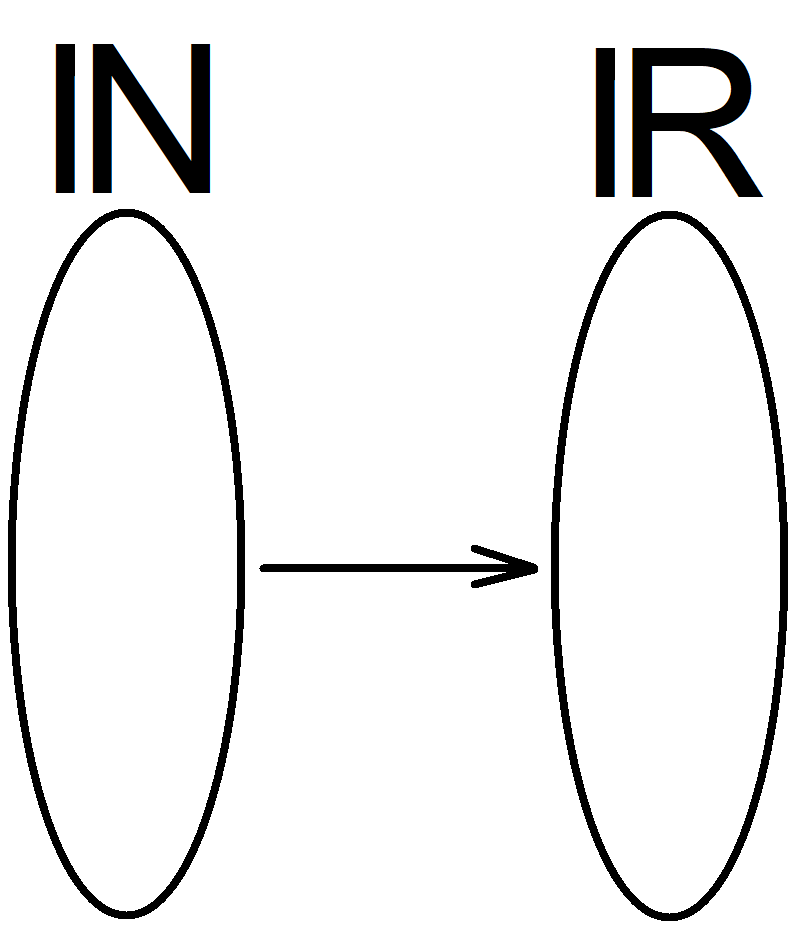
\includegraphics[width=0.2\textwidth]{img/lecture8/sequence}
	\end{center}
	Если поменять местами слагаемые ряда
	\begin{center}
		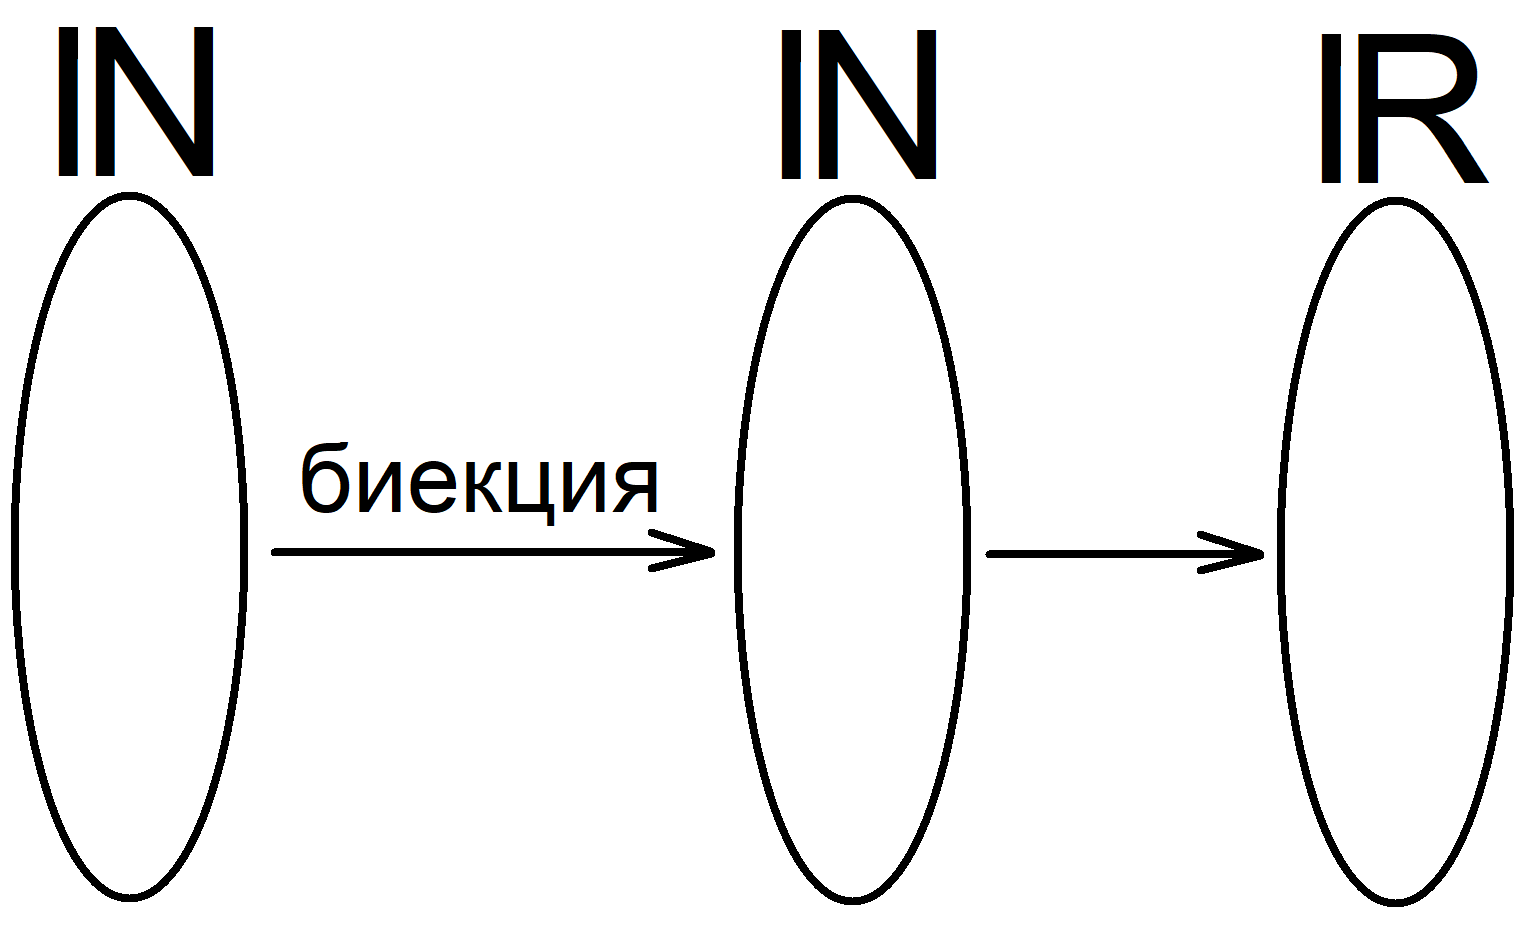
\includegraphics[width=0.4\textwidth]{img/lecture8/replacement_summands}
	\end{center}
	Функция $k(j)$ - биекция на $\N, k(j) = k_j$ $\{a_{k_j} | j \in \N\} = \{a_n | n \in \N\}$
	
	\begin{example}[семинарская задача 3.2]
		Если ряд сходится условно, то при перестановке членов его сумма может измениться.
		\[ 1 - 1 + \frac{1}{2} - \frac{1}{2} + \frac{1}{3} - \frac{1}{3} + \dots = 0 \]
		Переставим члены ряда
		\[ 1 + \frac{1}{2} - 1 + \frac{1}{3} + \frac{1}{4} - \frac{1}{2} + \dots = \sum_{k = 1}^{3n} \tilde{a_k} = \sum_{k = 1}^{2n} \frac{1}{k} - \sum_{k = 1}^n \frac{1}{k} = \ln{2n} + \gamma + \alpha_n - \ln{n} - \gamma' - \alpha'_n = \]
		\[ = \ln{2} + \gamma + \alpha_n - \gamma' - \alpha'_n \Rightarrow \text{ряд сходится к } \ln{2}, \text{ а не к нулю.} \]
	\end{example}
		
	\begin{definition}
		Будем говорить, что ряд $\sum_{j = 1}^{\infty} \tilde{a_j}$ получен перестановкой членов ряда $\sum_{k = 1}^{\infty} a_k$, если существует последовательность натуральных чисел $\{k_j\}^{\infty}_{j = 1}$, задающая взаимно однозначное преобразование (биекцию) множества $\N$, и такая, что $\forall j \in \N \rightarrow \tilde{a_j} = a_{k_j}$.
	\end{definition}
	
	\begin{theorem}[О независимости суммы абсолютно сходящегося ряда от порядка слагаемых]
		Если ряд $\sum^{\infty}_{j = 1} \tilde{a_j}$ получен перестановкой членов абсолютно сходящегося ряда $\sum^{\infty}_{k = 1} a_k$, то ряд $\sum^{\infty}_{j = 1} a_j$ абсолютно сходится и его сумма равна сумме ряда $\sum^{\infty}_{k = 1} a_k$.
	\end{theorem}
	
	\begin{proof}
		Краткая запись:
		\[ \sum^{\infty}_{j = 1} a_j \rightsquigarrow \sum^{\infty}_{j = 1} \tilde{a_j} = \sum^{\infty}_{j = 1} a_{k_j} \]
		\underline{Шаг 1} Рассмотрим случай, когда $a_k \geqslant 0$ $\forall k \in \N.$
		
		Для любого $n \in \N$ определим $\displaystyle M_n = \max_{j \in \{1, \dots, n\}} \{k_j\}.$
		
		Для любого $n \in \N$ имеем
		\[ \sum_{j = 1}^n \tilde{a_j} = \sum_{j = 1}^n a_{k_j} \leqslant \sum_{k = 1}^{M_n} a_k \leqslant \sum^{\infty}_{k = 1} a_k \text{ (*)} \]
		(последние два неравенства верны, потому что ряд с неотрицательными членами и $n \leqslant M_n$)
		
		Ряд $\sum^{\infty}_{k = 1} a_k$ - абсолютно сходящийся $\Rightarrow \sum^{\infty}_{k = 1} a_k$ - сходится.
		
		Частичные суммы $\sum^n_{j = 1} \tilde{a_j}$ не убывают (т. к. $a_k \geqslant 0$) и ограниченные числом $\sum^{\infty}_{k = 1} a_k \Rightarrow$ по теореме Вейерштрасса $\sum^{\infty}_{j = 1} \tilde{a_j}$ - сходится.
		
		Итак, $\tilde{A_n} = \sum^n_{j = 1} \tilde{a_j} \leqslant \sum^{\infty}_{j = 1} a_j = A$ $(A = const)$
		
		По теореме о переходе к пределу в неравенстве $\lim_{n \to \infty} \tilde{A_n} \leqslant \lim_{n \to \infty} A \Rightarrow \sum^{\infty}_{j = 1} \tilde{a_j} \leqslant \sum^{\infty}_{j = 1} a_j.$
		
		Поскольку ряд $\sum^{\infty}_{j = 1} a_j$ может быть получен из ряда $\sum^{\infty}_{j = 1} \tilde{a_j}$ обратной перестановкой слагаемых, то $\sum^{\infty}_{j = 1} a_j \leqslant \sum^{\infty}_{j = 1} \tilde{a_j}$. Поэтому при перестановке слагаемых ряда с неотрицательными членами его сумма не меняется.
		
		\underline{Шаг 2} Рассмотрим общий случай. Применяя утверждение шага 1 для сходимости ряда $\sum^{\infty}_{k = 1} |a_k|$, получаем сходимость ряда $\sum^{\infty}_{j = 1} |\tilde{a_j}|$. Поэтому ряд $\sum^{\infty}_{j = 1} \tilde{a_j}$  сходится абсолютно. Для любого $k \in \N$ обозначим через $a^+_k = \max\{a_k, 0\}, a^-_k = \max\{-a_k, 0\}.$ Тогда при всех $k \in \N$
		\[ a_k = a^+_k - a^-_k \text{ (если } a_k > 0, \text{ то } a^+_k = a_k, a^-_k = 0; \text{ если } a_k < 0, \text{ то } a^+_k = 0, a^-_k = -a_k), \]
		\[ |a_k| = a^+_k + a^-_k \text{ (тоже самое)}, 0 \leqslant a^+_k \leqslant |a_k|, 0 \leqslant a^-_k \leqslant |a_k|. \]
		В силу утверждения, доказанного на шаге 1,
		\[ \sum^{\infty}_{j = 1} \tilde{a}^+_j = \sum^{\infty}_{j = 1} a^+_{k_j} =  \sum^{\infty}_{k = 1} a^+_k, \sum^{\infty}_{j = 1} \tilde{a}^-_j = \sum^{\infty}_{j = 1} a^-_{k_j} =  \sum^{\infty}_{k = 1} a^-_k, \]
		причём эти ряды сходятся по признаку сравнения (в силу (*)). Поэтому
		\[ \sum^{\infty}_{j = 1} \tilde{a_j} = \sum^{\infty}_{j = 1} a_{k_j} = \sum^{\infty}_{j = 1} (a^+_{k_j} - a^-_{k_j}) = (**) \]
		Предел последовательности разности частичных сумм равен разности пределов частичных сумм
		\[ (**): \sum^{\infty}_{j = 1} a^+_{k_j} - \sum^{\infty}_{j = 1} a^-_{k_j} = \sum^{\infty}_{k = 1} a^+_k - \sum^{\infty}_{k = 1} a^-_k = \sum^{\infty}_{k = 1} (a^+_k - a^-_k) = \sum^{\infty}_{k = 1} a_k. \]
	\end{proof}
	
	Заметим, что при перестановке условно сходящегося ряда, вообще говоря, меняется. Более того, справедлива следующая теорема.
	
	\begin{theorem}[Теорема Римана]
		Если ряд $\sum^{\infty}_{k = 1} a_k$ сходится условно, то для любого $x \in \R \cup \{+\infty, -\infty\}$ можно так переставить члены ряда $\sum^{\infty}_{k = 1} a_k,$ что полученный $\sum^{\infty}_{j = 1} \tilde{a_j}$ будет иметь сумму равную $x$.
	\end{theorem}
	
	Без доказательства.
	
	\chapter{Предел функции}
	
	\section{Окрестности}
	
	\begin{definition}
		Пусть $\epsilon > 0$.
		\begin{itemize}
			\item Окрестностью радиуса $\epsilon$ (или $\epsilon$-окрестностью) точки
			$a \in \R$ называется множество
			\[ B_{\epsilon}(a) := \{x \in \R : |x - a| < \epsilon\} = (a - \epsilon, a + \epsilon). \]
			\item Проколотой $\epsilon$-окрестностью точки $a \in \R$ называется
			множество
			\[ B'_{\epsilon}(a) := B_{\epsilon}(a) \setminus \{a\} = (a - \epsilon, a) \cup (a, a + \epsilon). \]
		\end{itemize}
	\end{definition}
	
	\section{Внутренние, предельные и граничные точки}
	
	\begin{definition}
		\begin{itemize}
			\item Точка $a \in \R$ называется \underline{внутренней} точкой множества $M$, если она входит в это множество $M$ с некоторой своей окрестностью (т. е. найдется такое $\epsilon > 0$, что $B_{\epsilon}(a) \subset M$).
			\item Точка $a \in \R$ называется \underline{предельной} точкой множества $M$, если каждая ее проколотая окрестность имеет непустое пересечение с множеством $M$ (т. е. для каждого $\epsilon > 0$ пересечение $B'_{\epsilon}(a) \cap M \neq \varnothing$).
			\item Точка $a \in \R$ называется \underline{граничной} точкой множества $M$, если каждая ее окрестность имеет непустое пересечение как с множеством $M$, так и с его дополнением (т. е. для каждого $\epsilon > 0$ и $B_{\epsilon}(a) \cap M \neq \varnothing$ и $B_{\epsilon}(a) \cap (\R \setminus M) \neq \varnothing)$.
		\end{itemize}
	\end{definition}
	
	\begin{example}
		Например, для множества $M = (0, 1] \cup \{3\}$ точки $0, \frac{1}{2}, 1$ будут
		предельными, а точки $-1$ и $3$ не будут; точки $0, 1, 3$ будут граничными, а точки $-1$ и $\frac{1}{2}$ не будут.
	\end{example}
	
	\newpage
	
	\section*{Лекция 9: Предел функции}
	
	\begin{mention}
		Точка a является предельной для $M$ тогда и только тогда, когда найдется сходящаяся к $a$ последовательность $a_n \in M \setminus \{a\}$.
	\end{mention}
	
	\begin{proof}
		\begin{itemize}
			\item[$\Rightarrow$] Если $a$ предельная, то $\forall \epsilon > 0$ $B'_{\epsilon}(a) \cap M \neq \varnothing \Rightarrow \forall n$ $\epsilon = \frac{1}{n}$ $a_n (\neq a) \in B'_{\frac{1}{n}}(a) \cap M \neq \varnothing \Rightarrow 0 < |a_n - a| < \frac{1}{n}, \frac{1}{n} \to 0 \Rightarrow |a_n - a| \to 0 \Rightarrow a_n \to a.$
			\item[$\Leftarrow$] Если $a_n \in M \setminus \{a\}$ и $a_n (\neq a) \to a,$ то $\forall \epsilon > 0$ $\exists N: \forall n > N \rightarrow |a_n - a| < \epsilon$. 
			
			Т. к. $a_n \in M \setminus \{a\}$ и $(a_n \neq a \Rightarrow 0 < |a_n - a| < \epsilon),$ то $a_n \in B'_{\epsilon}(a)$ и $a_n \in M \Rightarrow B'_{\epsilon}(a) \cap M \neq \varnothing.$
		\end{itemize}
	\end{proof}
	
	\section{Предел функции по Коши}
	
	\begin{theorem}
		Пусть функция $f$ определена на некотором множестве $D \subset \R$ и пусть $a$ - предельная для $D$ точка. Число $A$ называется \underline{пределом} функции $f$ в точке $a$ (по множеству $D$), если для каждого $\epsilon > 0$ найдется такое $\delta > 0$, что $|f(x) - A| < \epsilon$ для каждого $x \in D \cap B'_{\delta}(a)$. Используют обозначения $\lim_{x \to a} f(x) = A$ или $f(x) \to A$ при $x \to a$.
	\end{theorem}
	
	C помощью кванторов определение можно записать так: $\lim_{x \to a} f(x) = A,$  если $\forall \epsilon > 0$ $\exists \delta > 0: \forall x \in D \cap B'_{\delta}(a) \to |f(x) - A| < \epsilon$ или, эквивалентно,
	\[ \forall \epsilon > 0 \text{ } \exists \delta > 0: \forall x \in D, 0 < |x - a| < \delta \rightarrow |f(x) - A| < \epsilon. \]
	
	\begin{center}
		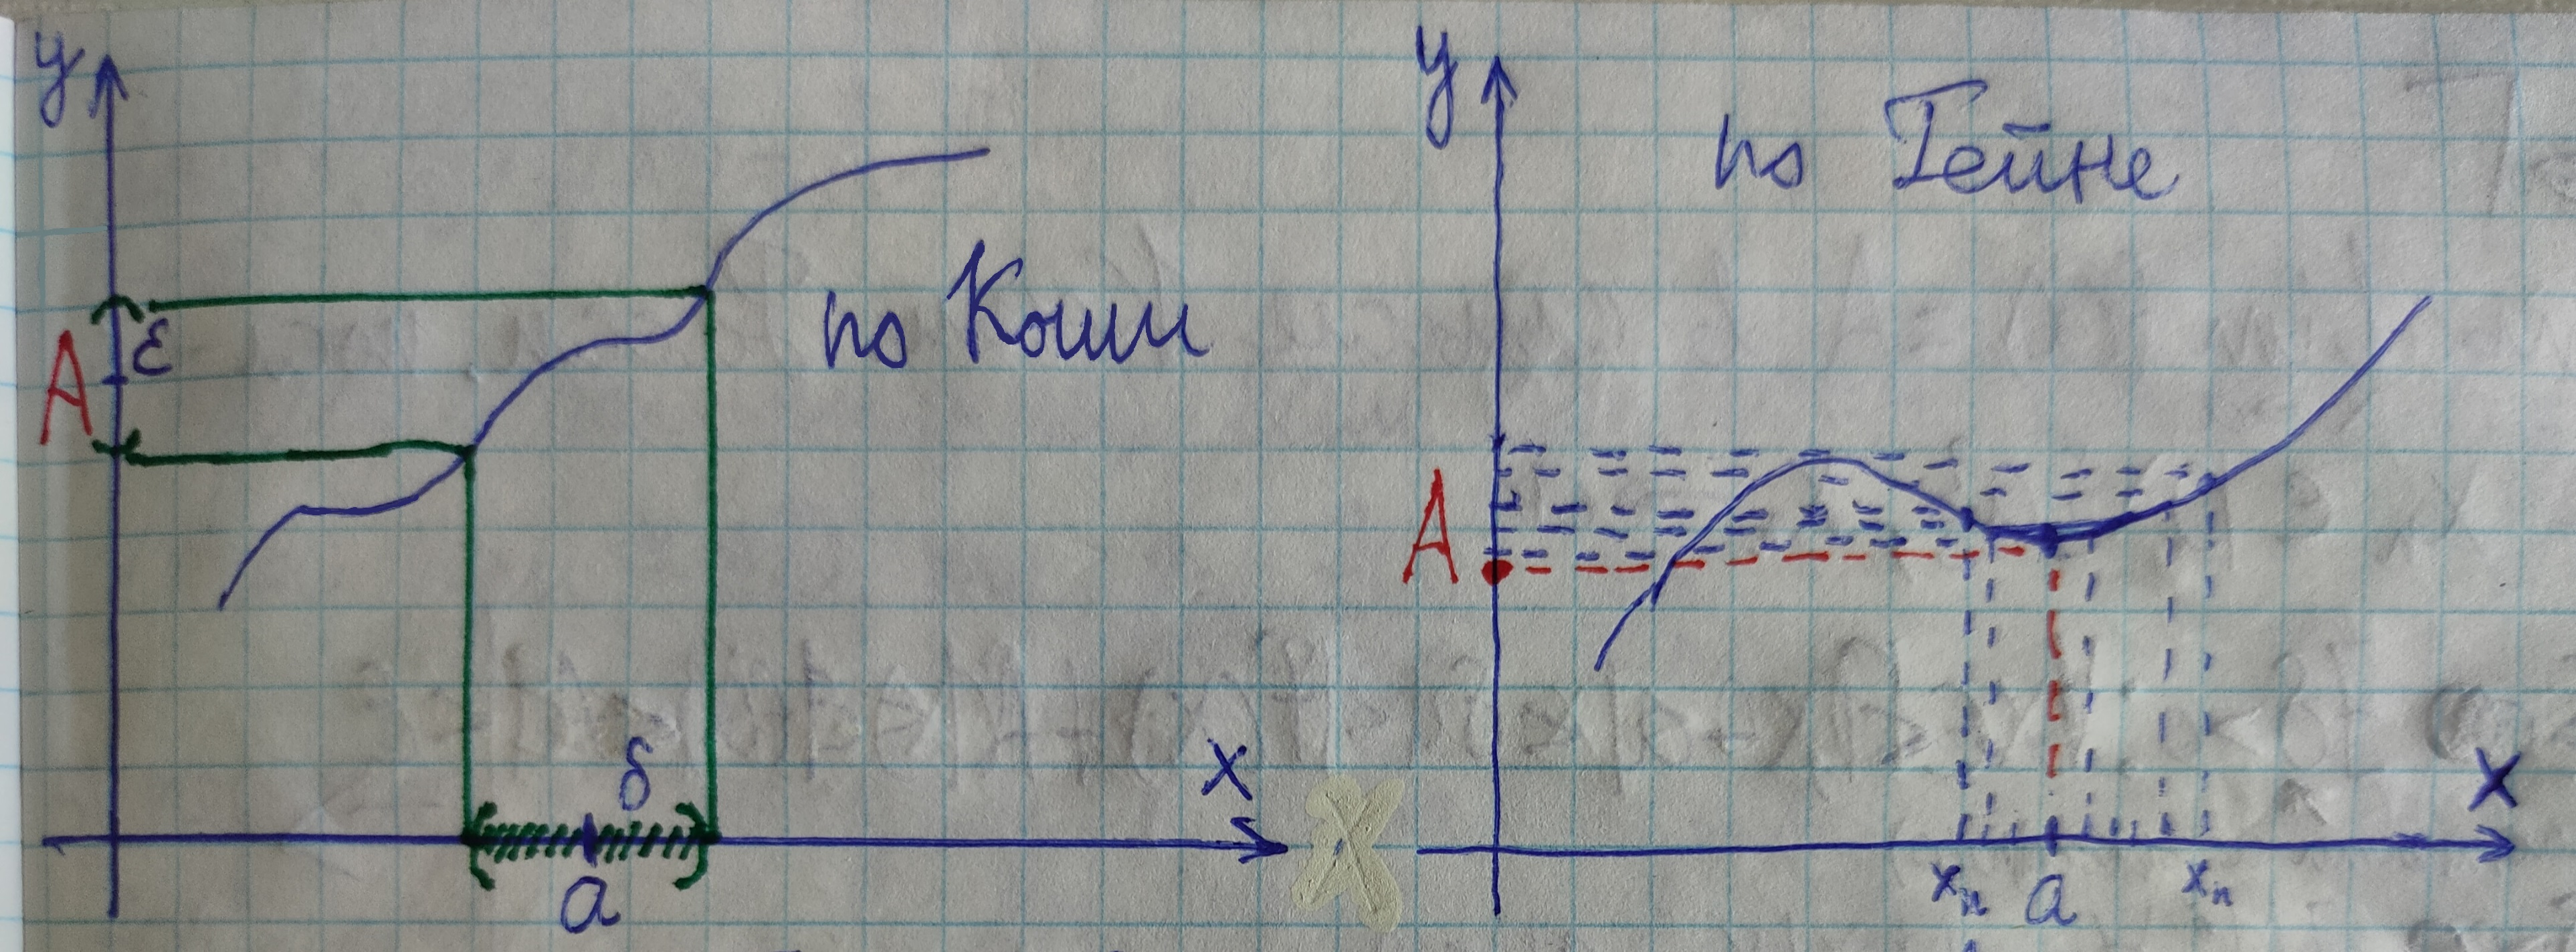
\includegraphics[width=0.7\textwidth]{img/lecture9/graphs}
	\end{center}
	
	\begin{example}
		Пусть $f(x) = x^2,$ тогда $\lim_{x \to 1} f(x) = 1.$
	\end{example}
	
	\begin{proof}
		Действительно, при $0 < |x - 1| < \delta$ выполнено $|f(x) - 1| = |x + 1||x - 1| < (\delta + 2)\delta$ $(|x + 1| \leqslant |x - 1| + 2 < \delta + 2).$ Поэтому при $\delta := \min\{1, \frac{\epsilon}{3}\}$ выполнено $|f(x) - 1| < \epsilon$ при каждом $x,$ для которого $0 < |x - 1| < \delta.$
		\begin{explanation}
			\begin{enumerate}
				\item $\delta = \frac{\epsilon}{3} < 1 \Rightarrow \epsilon < 3$
				
				$\delta(\delta + 2) = \frac{\epsilon}{3}(\frac{\epsilon}{3} + 2) < \frac{\epsilon}{3} (1 + 2) = \epsilon$
				\item $\delta = 1 \leqslant \frac{\epsilon}{3} \Rightarrow \epsilon \geqslant 3$
				
				$\delta(\delta + 2) = 3 \leqslant \epsilon$
			\end{enumerate}
		\end{explanation}
	\end{proof}
	
	\begin{example}
		Почему мы не берём сам предел в окрестность? А потому, что мы это используем при расчёте пределов:
		\[ \lim_{x \to 1} \frac{x^2 - 1}{x - 1} = \lim_{x \to 1} \frac{(x - 1)(x + 1)}{x - 1} = \lim_{x \to 1} (x + 1) = 2 \]
		
		Проверка: $(\forall \epsilon > 0) (\exists \delta > 0) (\forall x)$ $0 < |x - 1| < \delta$ $\big|\frac{x^2 - 1}{x - 1} - 2\big| < \epsilon$
		
		Примем $\delta := \epsilon: 0 < |x - 1| < \epsilon \Rightarrow \big|\frac{(x - 1)(x + 1)}{x - 1} - 2\big| = |x - 1| < \epsilon$
		
		Если мы бы допустили, что $a$ включено в $\delta$-окрестность, то никакое бы $\delta$ не подошло - для значения $x = a = 1$ было бы неверно, что $f(1) \in B_{\delta}(2).$
	\end{example}
	
	\begin{mention}
		Если множество $D$ не ограничено сверху (снизу), то можно определить предел функции в «точке» $+\infty$ $(-\infty)$. Для этого по определению будем считать, что $B'_{\epsilon}(+\infty) := (\frac{1}{\epsilon}, +\infty)$ и $B'_{\epsilon}(-\infty) := (-\infty, -\frac{1}{\epsilon}).$
	\end{mention}
	
	Можно дать альтернативное определение функции.
	
	\section{Предел функции по Гейне}
	
	\begin{theorem}
		Пусть функция $f$ определена на некотором множестве $D \subset \R$ и пусть $a$ предельная для $D$ точка. Число $A$ называется \underline{пределом} функции $f$ в точке $a$ (по множеству $D$), если для каждой последовательности точек $x_n \in D \setminus \{a\}$ $(x_n \neq a),$ $x_n \to a,$ выполнено $f(x_n) \to A$ при $n \to \infty.$
	\end{theorem}
	
	Покажем, что два этих определения задают один и тот же объект.
	
	\begin{theorem}
		Определения предела функции по Коши и по Гейне эквивалентны.
	\end{theorem}
	
	\begin{proof}
		\begin{enumerate}
			\item $\text{К} \Rightarrow \text{Г}$
			Пусть $\lim_{x \to a} f(x) = A$ в смысле Коши. Рассмотрим последовательность точек $x_n \in D \setminus \{a\}, x_n \to a.$
			\[ \lim_{x \to a} f(x) = A \Leftrightarrow \forall \epsilon > 0 \text{ } \exists \delta > 0: \forall x \in D, 0 < |x - a| < \delta \rightarrow |f(x) - A| < \epsilon \]
			\[ \lim_{n \to \infty} x_n = a \Leftrightarrow \forall \delta > 0 \text{ } \exists N: \forall n > N \text{ } |x_n - a| < \delta \]
			\item $\text{Г} \Rightarrow \text{К}$ От противного.
			
			Пусть число $A$ не является пределом функции $f$ в точке $a$ в смысле Коши. Это означает, что
			\[ \exists \epsilon > 0 \text{ } \forall \delta > 0: \exists x_{\delta} \in D, 0 < |x_{\delta} - a| < \delta \rightarrow |f(x_{\delta}) - A| \geqslant \epsilon \]
			(отрицание определения Коши)
			
			Рассмотрим последовательность $a_n = x_{\frac{1}{n}}$.
			
			Пусть $\delta = \frac{1}{n}.$ Тогда
			\[ \exists \epsilon > 0 \text{ } \forall \delta > 0: \exists a_n \in D, 0 < |a_n - a| < \frac{1}{n} \rightarrow |f(a_n) - A| \geqslant \epsilon \]
			$0 < |a_n - a| < \frac{1}{n} \Rightarrow$ по теореме о зажатой последовательности $a_n \to a,$ но последовательность точек $f(a_n)$ не сходится к $A$. Таким образом, число $A$ не является пределом функции $f$ в точке $a$ в смысле Гейне.
		\end{enumerate}
	\end{proof}
	
	\section{Арифметические свойства предела функции и неравенства}
	
	\begin{theorem}
		Пусть функции $f, g, h$ определены на некотором множестве $D \subset \R$ и пусть $а$ - предельная для $D$ точка. Тогда
		\begin{enumerate}
			\item (единственность предела) если $\displaystyle \lim_{x \to a} f(x) = A$ и $\displaystyle \lim_{x \to a} f(x) = B,$ то $A = B$;
			\item (линейность предела) если $\displaystyle \lim_{x \to a} f(x) = A$ и $\displaystyle \lim_{x \to a} g(x) = B,$ то $\displaystyle \lim_{x \to a} (\alpha f(x) + \beta g(x)) = \alpha A + \beta B$ $\forall \alpha, \beta \in \R;$
			\item (предел произведения) если $\displaystyle \lim_{x \to a} f(x) = A$ и $\displaystyle \lim_{x \to a} g(x) = B,$ то $\displaystyle \lim_{x \to a} (f(x) \cdot g(x)) = A \cdot B;$
			\item (предел отношения) если $\displaystyle \lim_{x \to a} f(x) = A, \lim_{x \to a} g(x) = B \neq 0$	и $g(x) \neq 0$ при $x \in D,$ то $\displaystyle \lim_{x \to a} \frac{f(x)}{g(x)} = \frac{A}{B};$
			\item (переход к пределу в неравенстве) если $\exists r > 0 : f(x) \leqslant g(x)$ при $x \in D \cap B'_r(a)$ и $\displaystyle \lim_{x \to a} f(x) = A, \lim_{x \to a} g(x) = B,$ то $A \leqslant B;$
			\item (предел зажатой функции) если $\exists r > 0 : f(x) \leqslant h(x) \leqslant g(x)$ при $x \in D \cap B'_r(a)$ и $\displaystyle \lim_{x \to a} f(x) = \lim_{x \to a} g(x) = A,$ то $\displaystyle \lim_{x \to a} h(x) = A;$
			\item (ограниченность функции) если $\displaystyle \lim_{x \to a} f(x) = A,$ то найдутся такие $\delta > 0$ и $C > 0,$ что $|f(x)| \leqslant C$ при каждом $x \in D \cap B'_{\delta}(a);$
			\item (отделимость от нуля) если $\displaystyle \lim_{x \to a} f(x) = A \neq 0,$ то найдется такое $\delta > 0,$ что $|f(x)| > \frac{|A|}{2}$ при $x \in D \cap B'_{\delta}(a).$
		\end{enumerate}
	\end{theorem}
	
	\begin{proof}
		Свойства 1) - 6) следуют из аналогичных свойств для предела последовательности и определения функции по Гейне.
		
		7) При $\epsilon = 1 > 0$ $\exists \delta > 0: \forall x \in D \cap B'_{\delta}(a)$ $|f(x) - A| < 1 \Rightarrow |f(x)| - |A| \leqslant |f(x) - A| < 1 \Rightarrow |f(x)| \leqslant |A| + 1 = C > 0$
		
		8) При $\epsilon = \frac{|A|}{2} > 0$ $\exists \delta > 0: \forall x \in D \cap B'_{\delta}(a)$ $|f(x) - A| < \frac{|A|}{2} \Rightarrow |A - f(x)| < \frac{|A|}{2} \Rightarrow |A| - |f(x)| \leqslant |A - f(x)| < \frac{|A|}{2} \Rightarrow |f(x)| > \frac{|A|}{2}.$
	\end{proof}
	
	\section{Теорема о пределе сложной функции}
	
	\begin{theorem}
		Пусть $f : D \rightarrow E, g : E \rightarrow \R$, $a$ - предельная точка множества
		$D$, $b$ - предельная точка множества $E$, $\lim_{x \to a} f(x) = b, \lim_{y \to b} g(y) = с$ и есть такая проколотая окрестность $B'_{\delta}(a)$ точки $a$, что $f(x) \neq b$ для каждой точки $x \in B'_{\delta}(a) \cap D.$ Тогда $\lim_{x \to a} g(f(x)) = c.$
	\end{theorem}
	
	\begin{center}
		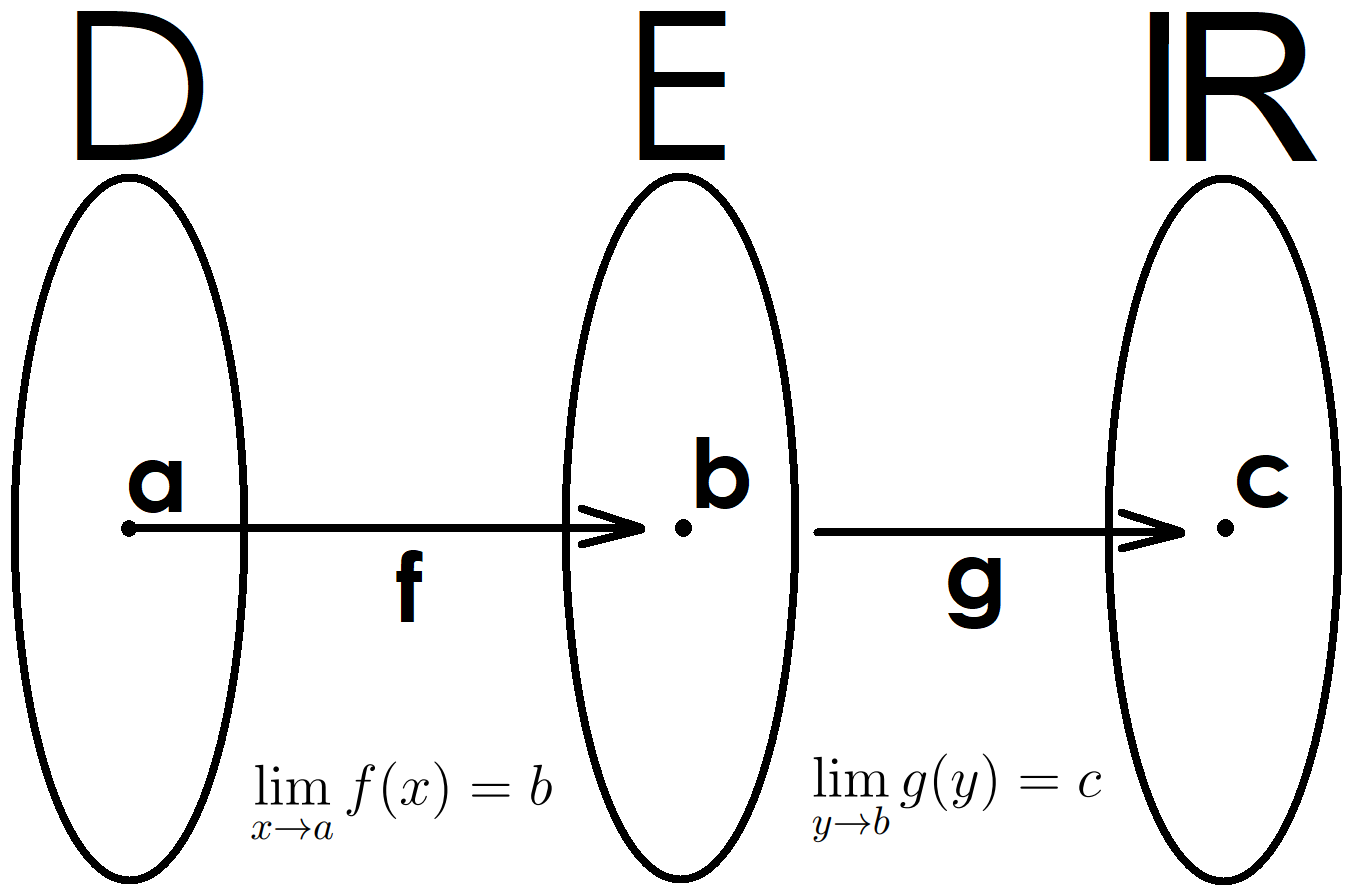
\includegraphics[width=0.5\textwidth]{img/lecture9/function_composition}
	\end{center}
	
	\begin{proof}
		$h(x) = g(f(x))$
		
		$\lim_{x \to a} f(x) = b \Rightarrow \forall \{x_n\}^{\infty}_{n = 1} \subset D \setminus \{a\}$ при $x_n \to a$ $y_n = f(x_n) \to b.$
		
		$x_n \to a$ и $\exists \delta > 0: \forall x \in B'_{\delta}(a) \to f(x) \neq b \Rightarrow$
		
		$\Rightarrow \exists N: \forall n \geqslant N \rightarrow x_n \in B'_{\delta}(a)$ $(\epsilon = \delta)$ и $f(x_n) \neq b.$
		
		Тогда последовательность $\{f(x_n)\}^{\infty}_{n = N} \subset E \setminus \{b\}$ и $f(x_n) \to b \Rightarrow$
		
		 $\Rightarrow$ (из $\lim_{x \to b} g(x) = c$) $g(f(x_n)) \to c.$
	\end{proof}
	
	\newpage	
	
	\section*{Лекция 10: Замечательные пределы, критерий Коши}
	
	\section{Первый замечательный предел}
	
	\begin{sentence}
		$\displaystyle \lim_{x \to 0} \frac{\sin{x}}{x} = 1.$
	\end{sentence}
	
	\begin{proof}
		\begin{enumerate}
			\item $x \in \big(0; \frac{\pi}{2}\big)$
			\begin{center}
				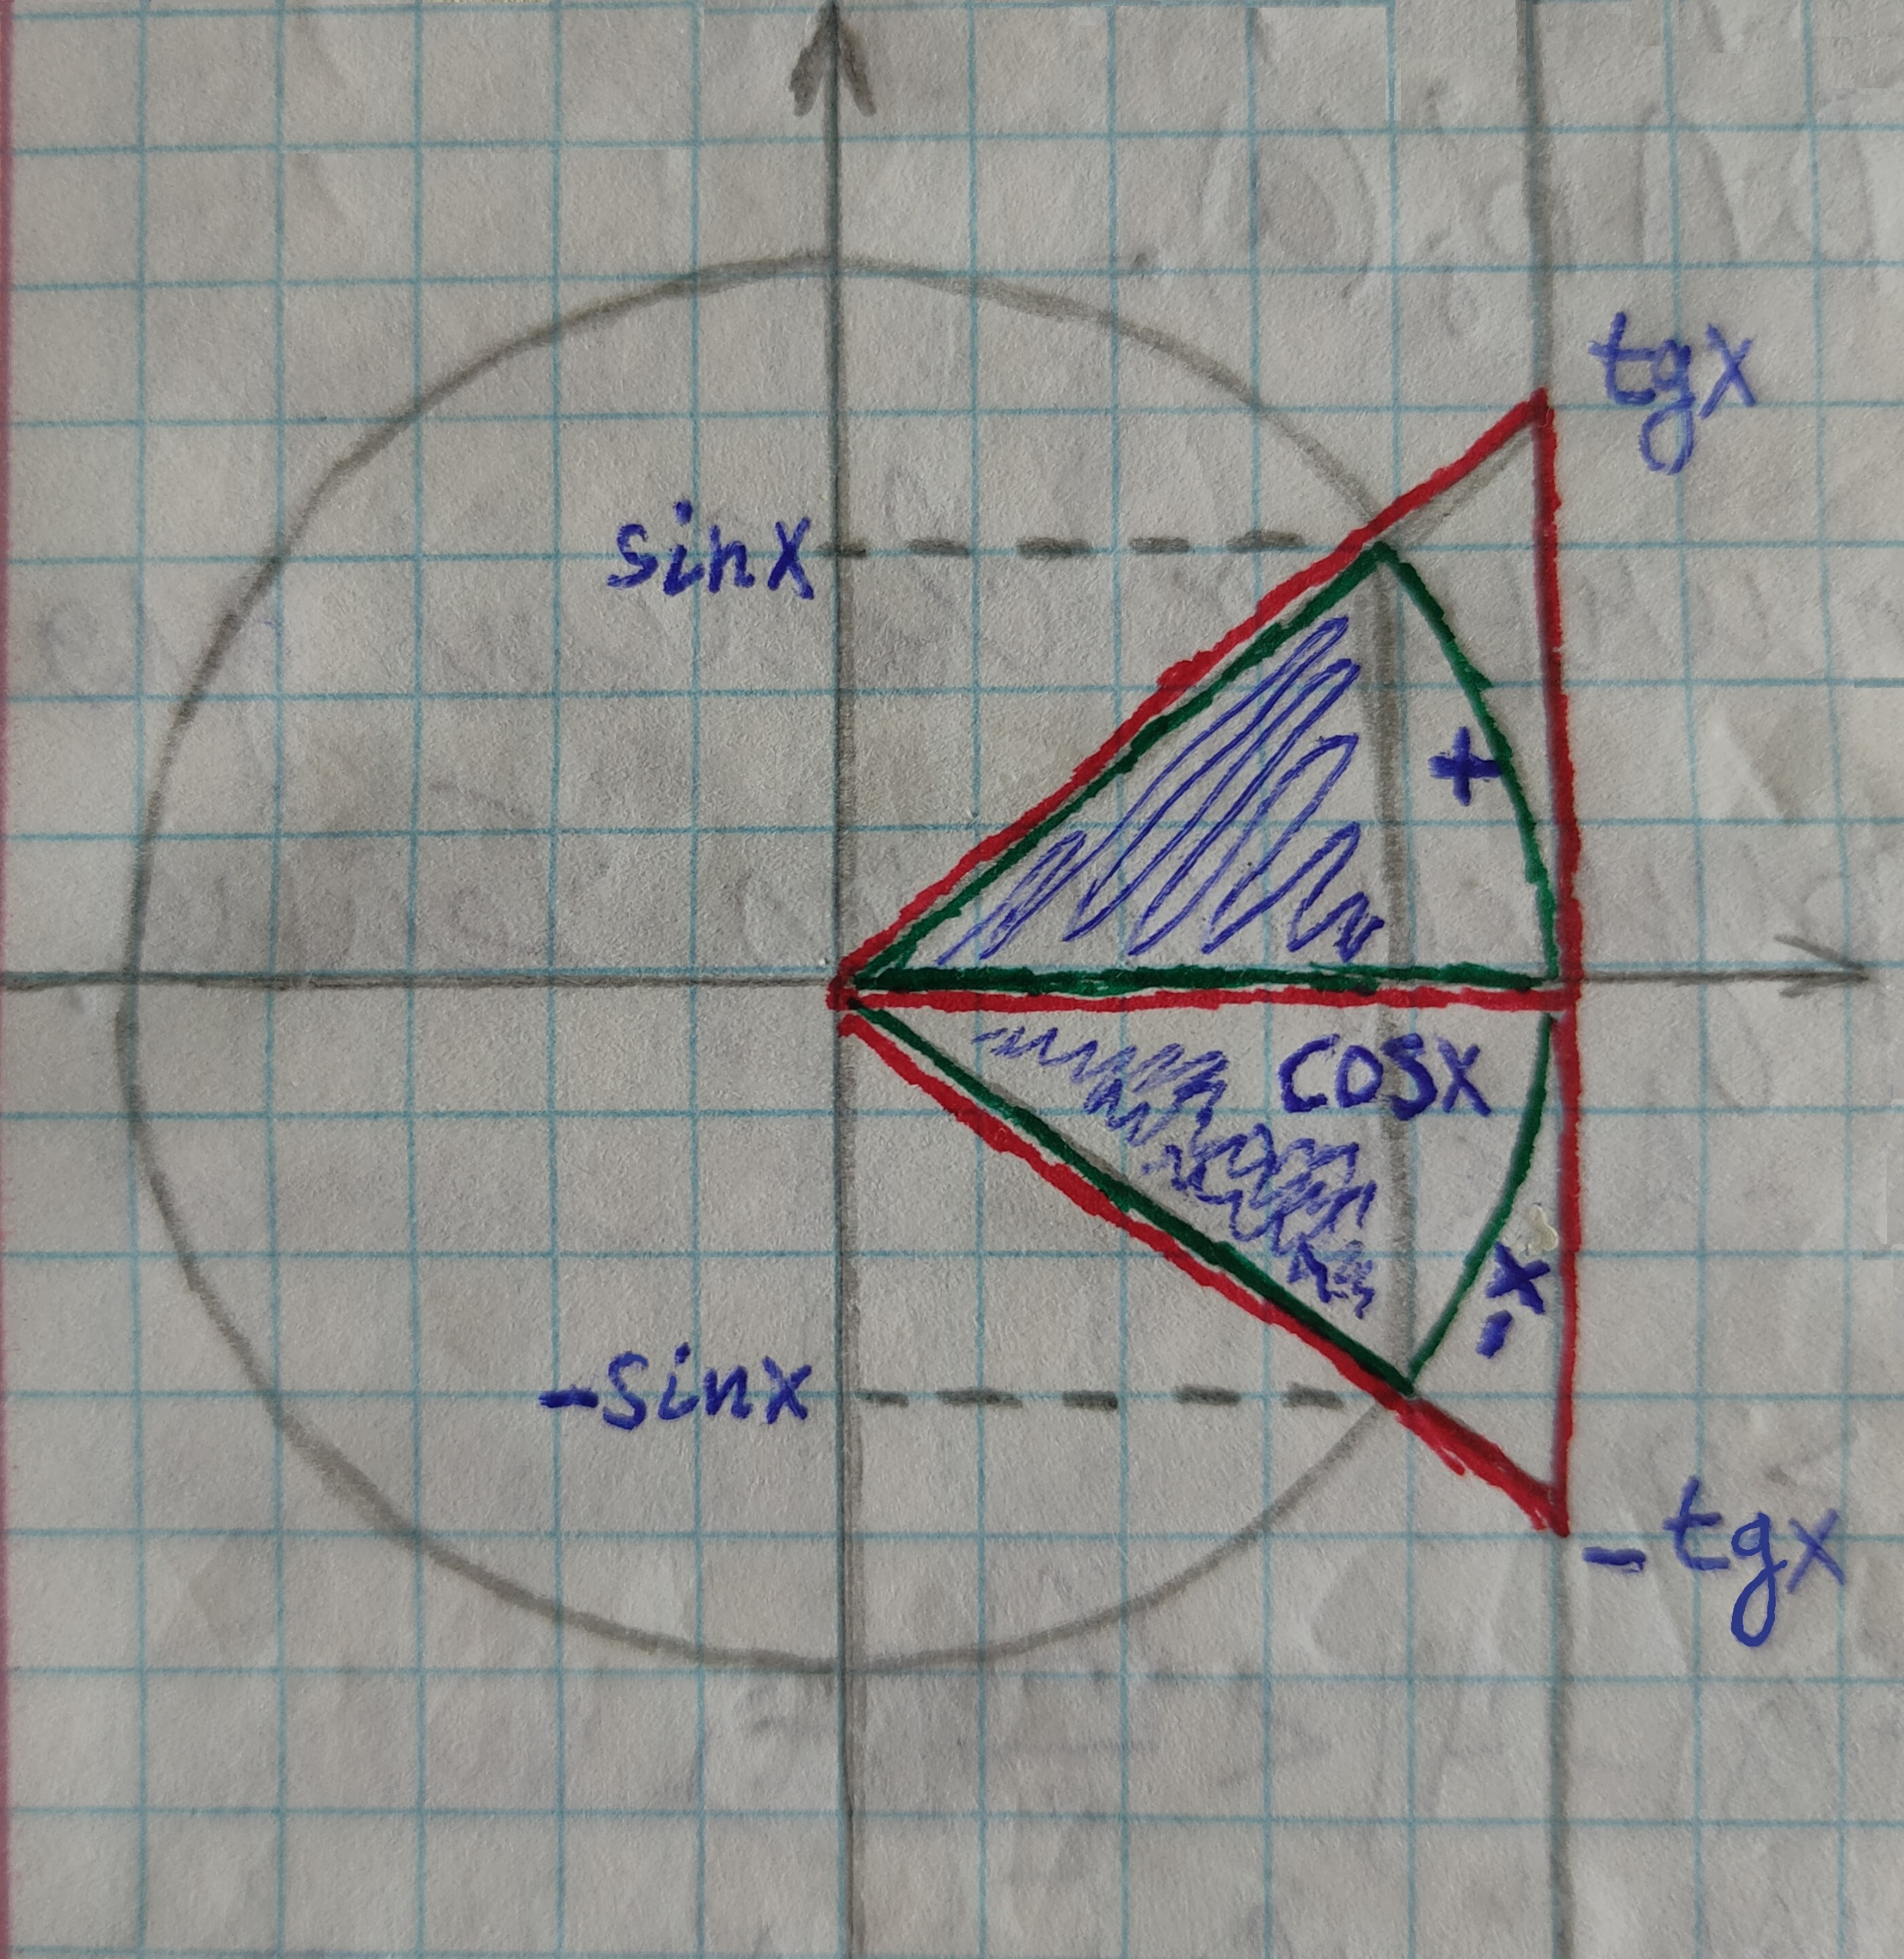
\includegraphics[width=0.4\textwidth]{img/lecture10/first_wonderful_limit}
			\end{center}
			\[ S_{\text{с}} \leqslant S_{\text{з}} \leqslant S_{\text{к}} \text{ - площади синего, зелёного и красного треугольников} \]
			
			Используем формулу площади прямоугольного треугольника $S_{\text{с}} = \frac{1}{2} \cdot \sin{x} \cdot \cos{x}, S_{\text{к}} = \frac{\tg{x}}{2}$, а затем $x$-ой части круга $S_{\text{з}} = \frac{x}{2\pi} \cdot \pi \cdot 1^2$.	
			\[ \frac{1}{2} \cdot \sin{x} \cdot \cos{x} < \frac{x}{2\pi} \cdot \pi \cdot 1^2 = \frac{x}{2} < \frac{\tg{x}}{2} \text{ } | \cdot 2 \]
			\[ \sin{x} \cdot \cos{x} < x < \tg{x} = \frac{\sin{x}}{\cos{x}} \]
			\[ \sin{x} \cdot \cos{x} < x \text{ } | : x > 0 \Rightarrow \frac{\sin{x}}{x} \cdot \cos{x} < 1 \text{ } | : \cos{x} > 0 \Rightarrow \frac{\sin{x}}{x} < \frac{1}{\cos{x}} \]
			\[ x < \frac{\sin{x}}{\cos{x}} \text{ } | \cdot \cos{x} > 0 \Rightarrow x \cdot \cos{x} < \sin{x} \text{ } | : x > 0 \Rightarrow \cos{x} < \frac{\sin{x}}{x} \]
			\[ \cos{x} < \frac{\sin{x}}{x} < \frac{1}{\cos{x}} \]
			$\displaystyle \lim_{x \to 0} \cos{x} = 1, \lim_{x \to 0} \frac{1}{\cos{x}} = 1 \Rightarrow \lim_{x \to 0} \frac{\sin{x}}{x} = 1$ по теореме о зажатой функции.
			\item $x \in \big(-\frac{\pi}{2}; 0\big)$
			\[ -\frac{1}{2} \cdot \sin{x} \cdot \cos{x} < -\frac{x}{2\pi} \cdot \pi \cdot 1^2 = -\frac{x}{2} < -\frac{\tg{x}}{2} \]
			\[ \sin{x} \cdot \cos{x} > x > \tg{x} = \frac{\sin{x}}{\cos{x}} \]
			\[ \sin{x} \cdot \cos{x} > x \text{ } | : x < 0 \Rightarrow \frac{\sin{x}}{x} \cdot \cos{x} < 1 \text{ } | : \cos{x} > 0 \Rightarrow \frac{\sin{x}}{x} < \frac{1}{\cos{x}} \]
			\[ x > \frac{\sin{x}}{\cos{x}} \text{ } | \cdot \cos{x} > 0 \Rightarrow x \cdot \cos{x} > \sin{x} \text{ } | : x < 0 \Rightarrow \cos{x} < \frac{\sin{x}}{x} \]
			\[ \cos{x} < \frac{\sin{x}}{x} < \frac{1}{\cos{x}} \]
			
			Осталось доказать, что $\lim_{x \to y} \cos{x} = \cos{y},$ т. е. функция непрерывна (предел в этой точке равен значению функции в этой точке)
			
			Требуется доказать $\displaystyle \lim_{x \to y} \cos{x} = \cos{y}.$
			\[ \forall \epsilon > 0 \text{ } \exists \delta > 0: \forall x \in D, 0 < |x - y| < \delta \rightarrow |\cos{x} - \cos{y}| < \epsilon \]
			\[ |\cos{x} - \cos{y}| = \bigg|2\sin{\bigg(\frac{x + y}{2}\bigg)}\sin{\bigg(\frac{x - y}{2}\bigg)}\bigg| \leqslant 2\bigg|\sin{\bigg(\frac{x - y}{2}\bigg)}\bigg| \leqslant 2\bigg|\frac{x - y}{2}\bigg| = |x - y| \]
			Здесь мы пользуемся неравенством $|\sin{\alpha}| \leqslant |\alpha|$
			\begin{center}
				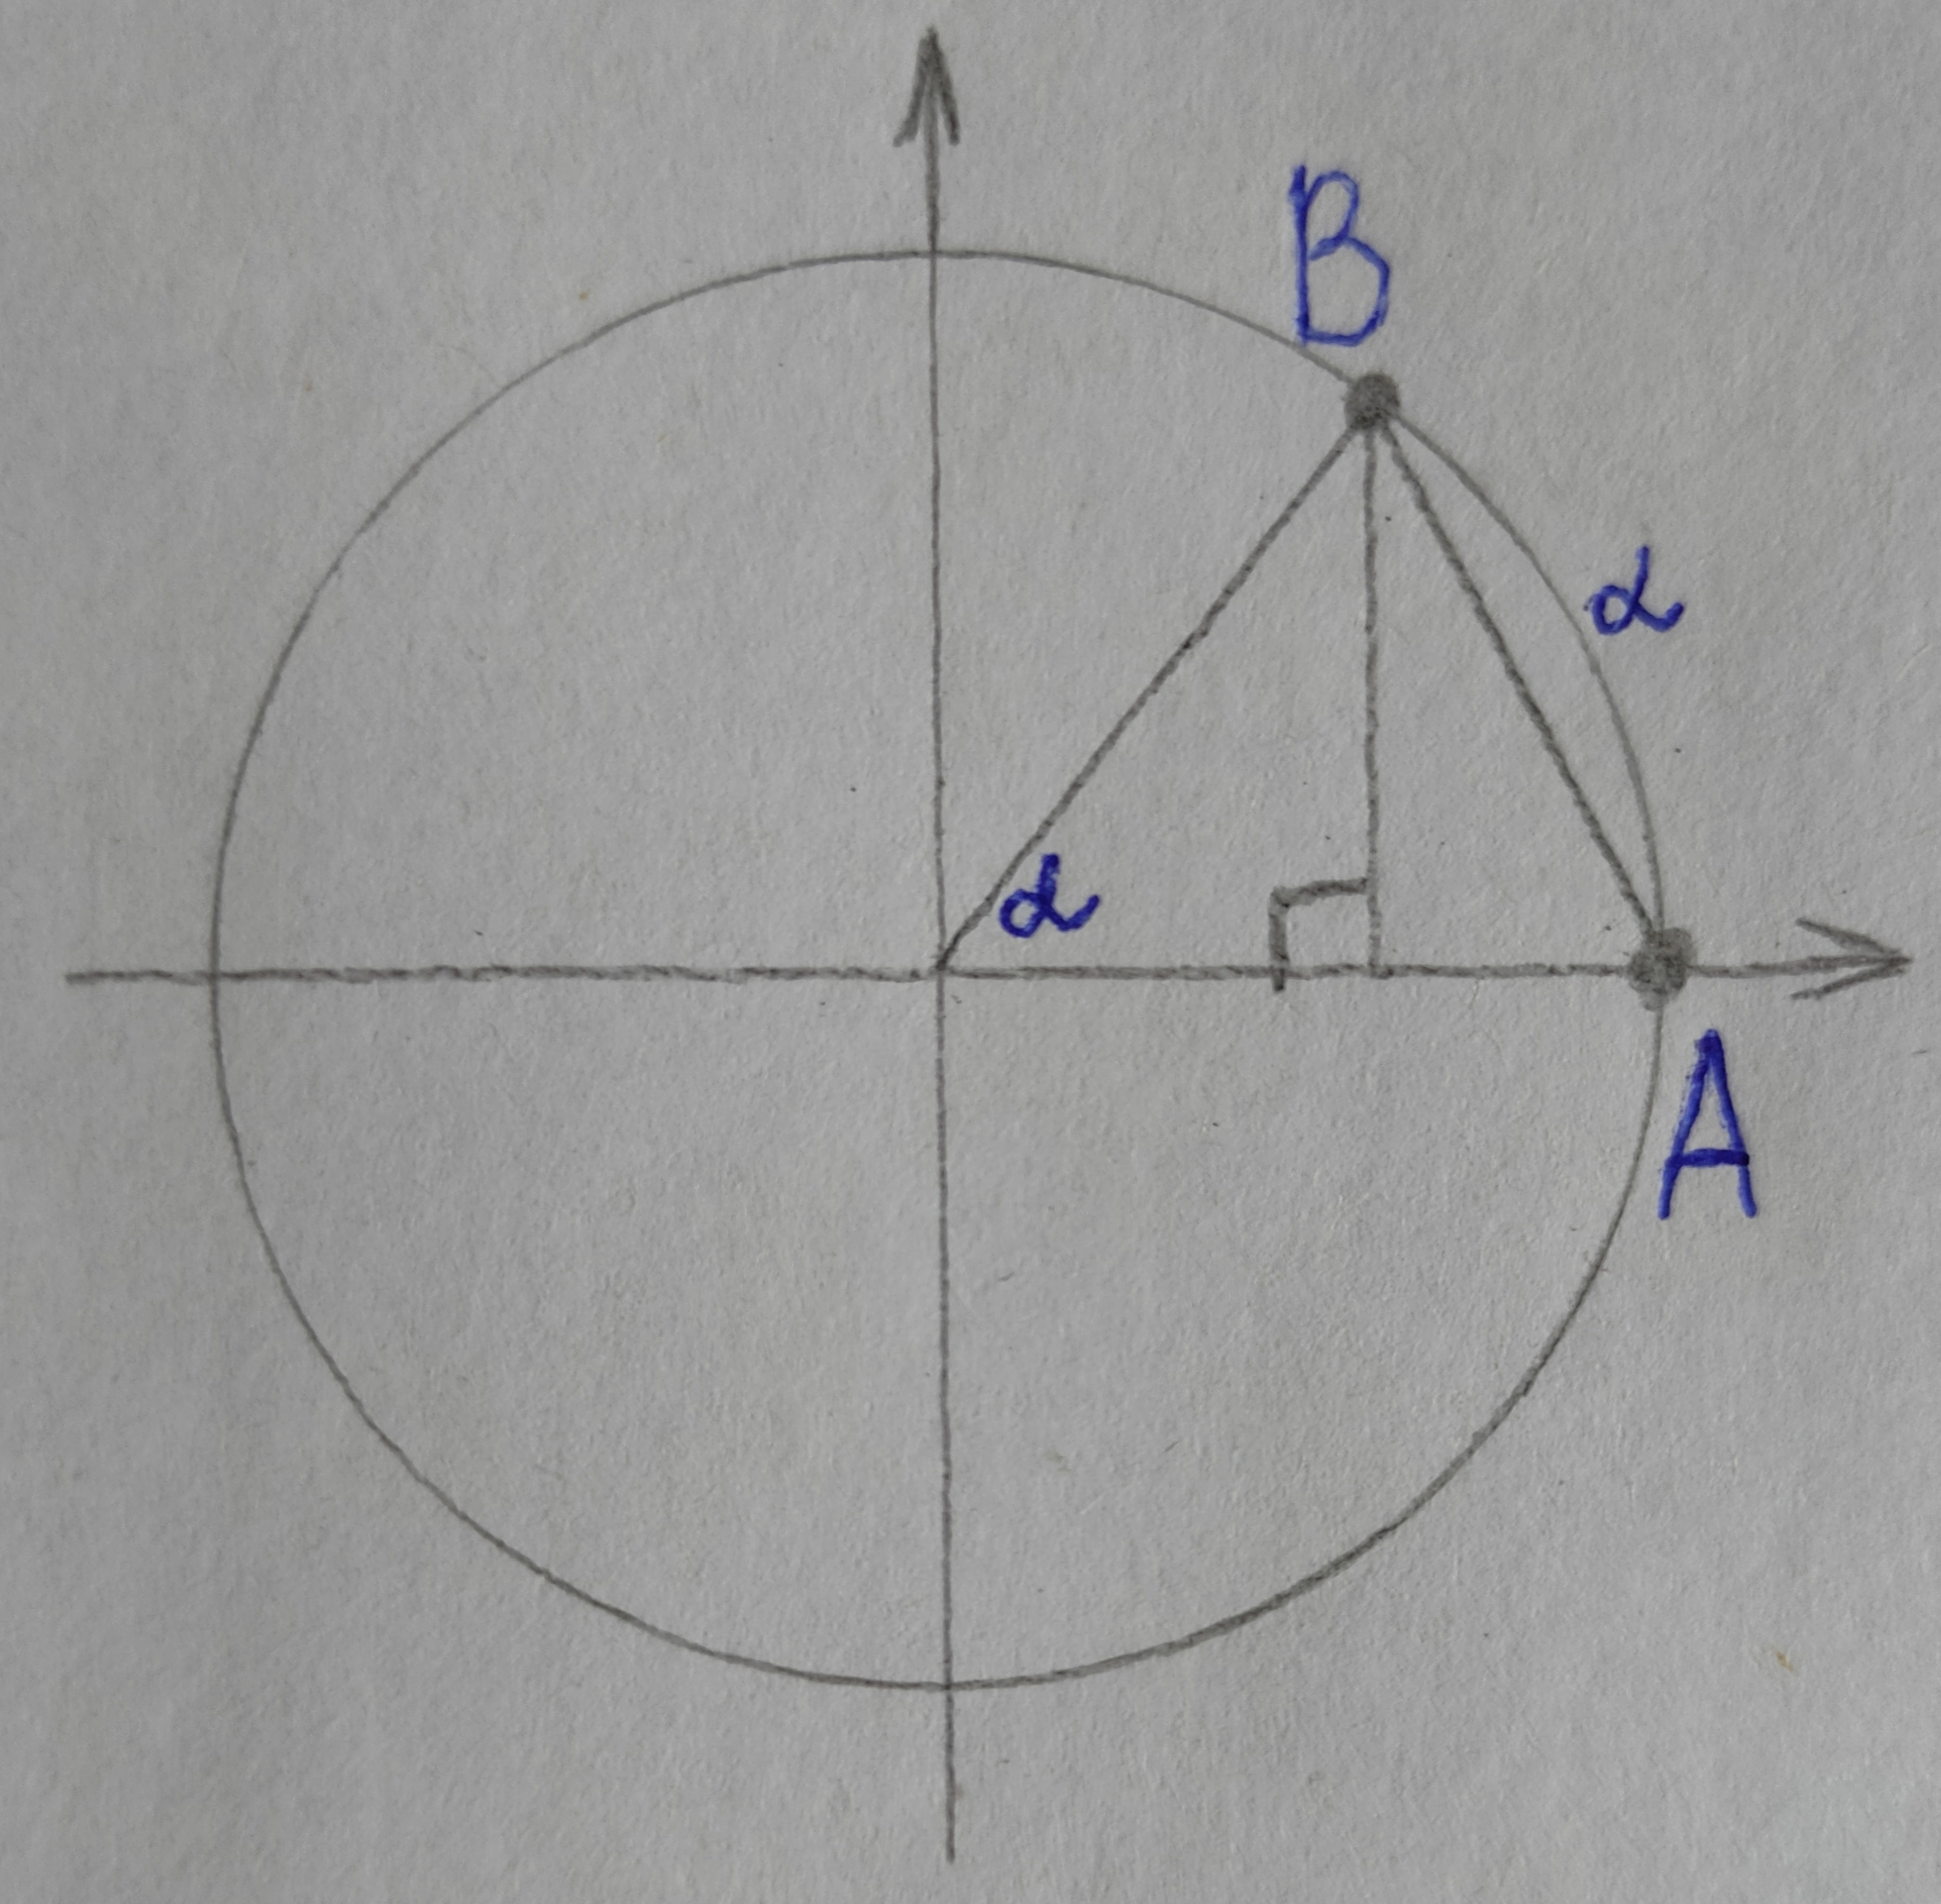
\includegraphics[width=0.2\textwidth]{img/lecture10/sin_inequality}
			\end{center}
			Дуга больше отрезка $AB$. Отрезок больше высоты. Поэтому дуга угла $\alpha$ больше синуса соответствующего угла (или равна, если $A = B$).
			
			Тогда если взять $\delta = \frac{\epsilon}{2},$ то $|x - y| \leqslant \frac{\epsilon}{2} < \epsilon \Rightarrow |\cos{x} - \cos{y}| < \epsilon.$ 
		\end{enumerate}
	\end{proof}
	
	\section{Второй замечательный предел}
	
	\begin{sentence}
		$\displaystyle \lim_{x \to +\infty} \bigg(1 + \frac{1}{x}\bigg)^x = e.$
	\end{sentence}
	
	\begin{proof}
		Пусть $f(x) := \big(1 + \frac{1}{1 + [x]}\big)^{[x]}, g(x) := \big(1 + \frac{1}{[x]}\big)^{[x] + 1}.$
		
		Тогда $f(x) \leqslant \big(1 + \frac{1}{x}\big)^x \leqslant g(x).$
		
		Кроме того, 
		\[ \lim_{n \to +\infty} \bigg(1 + \frac{1}{n + 1}\bigg)^n = \lim_{n \to +\infty} \frac{\big(1 + \frac{1}{n + 1}\big)^{n + 1}}{\big(1 + \frac{1}{n + 1}\big)} = \frac{e}{1} = e, \]
		\[ \lim_{n \to +\infty} \bigg(1 + \frac{1}{n}\bigg)^{n + 1} = \lim_{n \to +\infty} \bigg(1 + \frac{1}{n}\bigg)^n \bigg(1 + \frac{1}{n}\bigg) = e \cdot 1 = e. \]
		
		Следовательно, $\displaystyle \lim_{x \to +\infty} f(x) = \lim_{x \to +\infty} g(x) = e.$
		
		Утверждение следует из теоремы о пределе зажатой функции.
	\end{proof}
	
	\section{Критерий Коши}
	
	\begin{theorem}
		Пусть $f : D \rightarrow \R$ и $a$ - предельная точка $D$. Предел $\lim_{x \to a} f(x)$ существует тогда и только тогда, когда для каждого $\epsilon > 0$ найдется такое $\delta > 0$, что для каждых $x, y \in B'_{\delta}(a) \cap D$ выполнено $|f(x) - f(y)| < \epsilon$.
	\end{theorem}
	
	\begin{proof}
		\begin{itemize}
			\item[$\Rightarrow$] Пусть $\lim_{x \to a} f(x) = A \Rightarrow \forall \epsilon > 0$ $\exists \delta > 0: \forall x \in D,$
			
			$0 < |x - a| < \delta \rightarrow |f(x) - A| < \frac{\epsilon}{2}.$
			
			Тогда $|f(x) - A| < \frac{\epsilon}{2}, |f(y) - A| < \frac{\epsilon}{2} \Rightarrow |f(x) - f(y)| = |f(x) - A + A - f(y)| \leqslant |f(x) - A| + |A - f(y)| < \frac{\epsilon}{2} + \frac{\epsilon}{2} = \epsilon.$
			\item[$\Leftarrow$] Пусть $\forall \epsilon > 0$ $\exists \delta > 0: \forall x, y \in B'_{\delta}(a) \cap D \rightarrow |f(x) - f(y)| < \epsilon.$ Рассмотрим произвольную последовательность $\{x_n\}^{\infty}_{n = 1} \subset D \setminus  \{a\}, x_n \to a.$ Тогда $f(x_n)$ - фундаментальна (т. к. $\exists N: \forall n \geqslant N, x_n \in B'_{\delta}(a) \cap D \Rightarrow \forall n, m > N \rightarrow |f(x_n) - f(x_m)| < \epsilon) \Rightarrow\exists \lim_{n \to \infty} f(x_n) = A.$
			
			Пусть есть другая последовательность $\{y_n\}^{\infty}_{n = 1} \subset D \setminus \{a\}, y_n \to a.$
			
			Рассмотрим последовательность $z_{2k - 1} = x_k, z_{2k} = y_k,$ т. е. это последовательность вида $x_1, y_1, ... \subset D \setminus \{a\}.$
			
			\begin{tabular}{c|c}
				$x_n \to a \Rightarrow \forall \epsilon > 0$ $\exists N_1: \forall n \geqslant N_1 \rightarrow |x_n - a| < \epsilon$ & \multirow{2}*{$\Rightarrow \forall \epsilon > 0$ $\exists N_3 = 2\max\{N_1, N_2\}:$} \\
				$y_n \to a \Rightarrow \forall \epsilon > 0$ $\exists N_2: \forall n \geqslant N_2 \rightarrow |y_n - a| < \epsilon$ &                  
			\end{tabular}
			$\forall n \geqslant N_3 \rightarrow |z_n - a| < \epsilon \Rightarrow z_n \to a \Rightarrow$ (из определения предела функции по Гейне) $\lim_{n \to \infty} f(z_n) = B.$
			
			Но т. к. подпоследовательность $f(x_n)$ последовательности $f(z_n)$ сходится к $A$, то вся последовательность $f(z_n)$ сходится к $A = B.$ Значит $\lim_{x \to a} f(x)$ единственный. Таким образом, доказано существование предела по Гейне.
		\end{itemize}
	\end{proof}
	
	\newpage
	
	\section*{Лекция 11: Эквивалентность и o-символика}
	
	\section{Пределы справа и слева}
	
	Пусть $D^+_a := D \cap (a, +\infty)$ и $D^-_a := D \cap (-\infty, a).$
	
	\begin{definition}
		Пусть точка $a$ - предельная для множества $D^+_a$ и существует предел функции $f$ по множеству $D^+_a$ в точке $a$. Этот предел называют пределом справа функции $f$ в точке $a$ и обозначают $\lim_{x \to a + 0} f(x)$. Аналогично определяется предел слева, который обозначают $\lim_{x \to a - 0} f(x)$.
	\end{definition}
	\[ \lim_{x \to a + 0} f(x) = A, \lim_{x \to a - 0} f(x) = B \]
	\begin{center}
		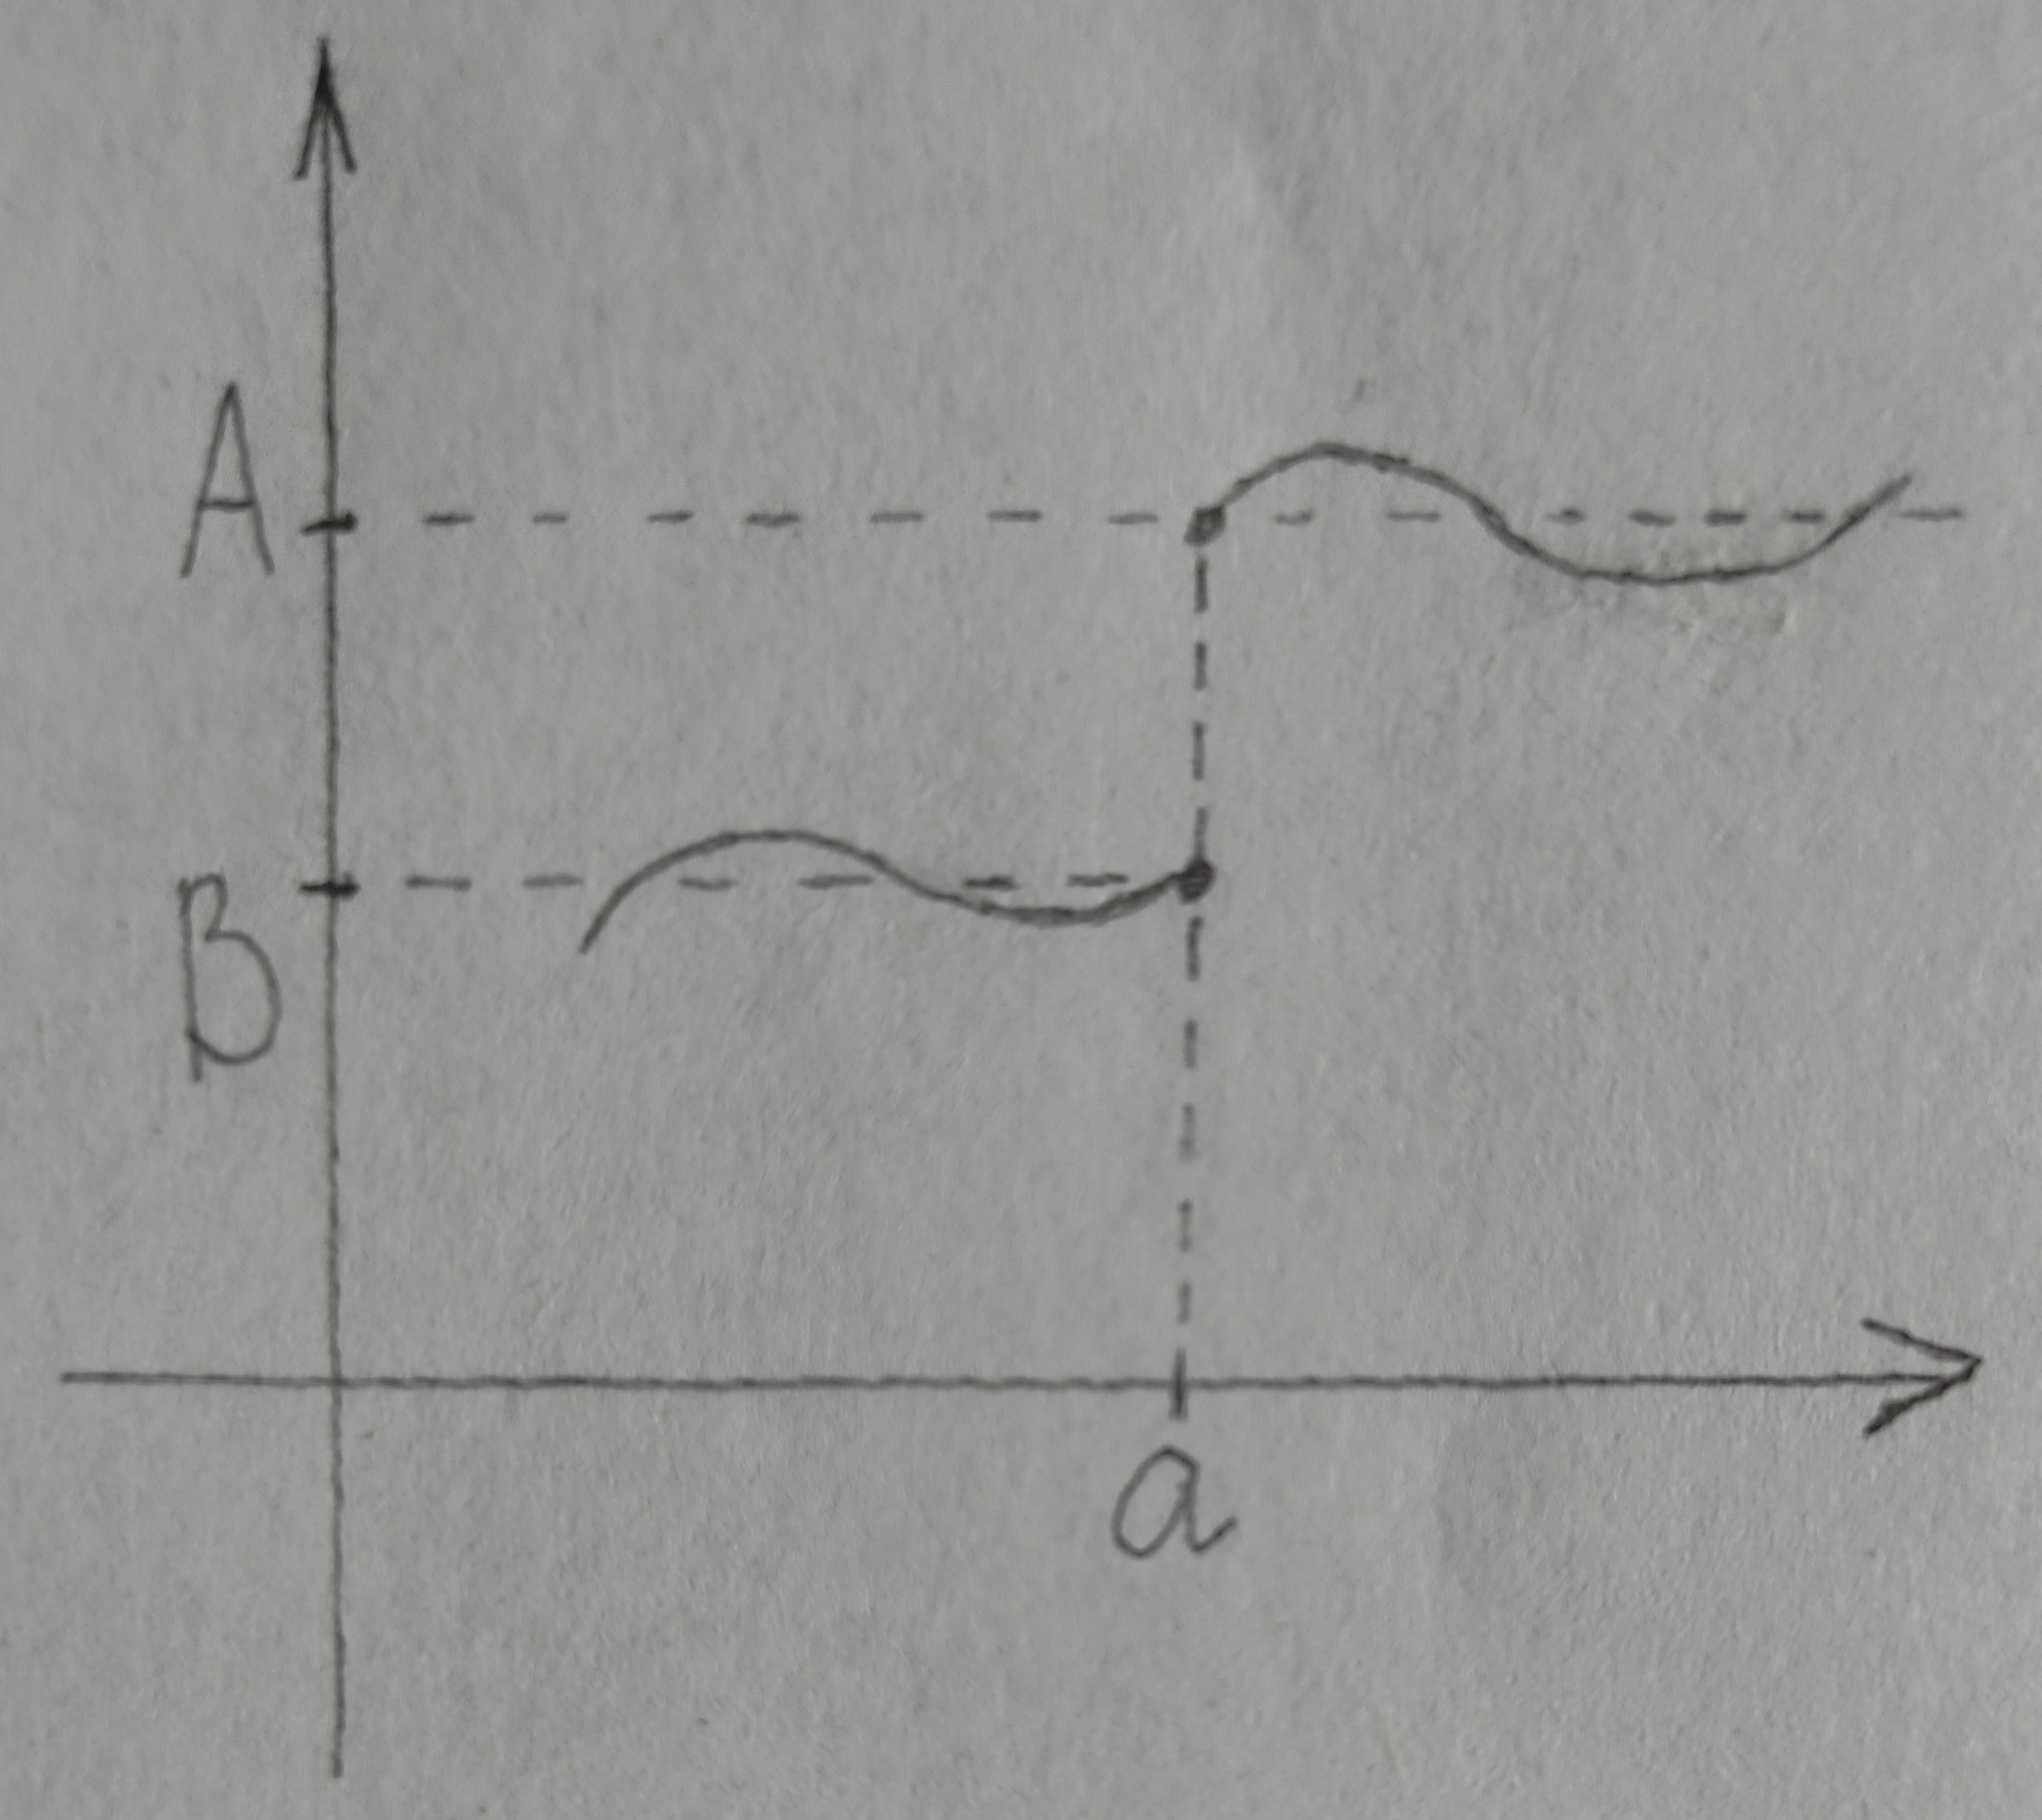
\includegraphics[width=0.3\textwidth]{img/lecture11/right_and_left_limit}
	\end{center}
	
	\section{Теорема Вейерштрасса}
	
	\begin{theorem}
		Пусть $f$ - не убывает и ограничена на множестве $D$, $a$ - предельная точка множества $D^-_a$. Тогда существует предел слева
		\[ \lim_{x \to a - 0} f(x) = \sup\{f(x) : x \in D^-_a\}. \]
		Пусть $f$ - не убывает и ограничена на множестве $D$, $a$ - предельная точка множества $D^+_a$. Тогда существует предел справа
		\[ \lim_{x \to a + 0} f(x) = \inf\{f(x) : x \in D^+_a\}. \]
		Аналогичные утверждения с заменой $\inf$ на $\sup$ справедливы и для невозрастающей функции.
	\end{theorem}
	
	\begin{proof}
		Пусть $M = \sup_{x \in D^-_a} f(x).$
		\begin{enumerate}
			\item $\forall \epsilon > 0$ $\exists x_0 \in D^-_a : f(x_0) > M - \epsilon$
			
			\underline{Пояснение.} $M = \sup{A}$
			\begin{enumerate}
				\item $\forall a \in A$ $a \leqslant M$
				\item $\forall b$ - верхняя грань $A \rightarrow b \geqslant M$
			\end{enumerate}
			$\forall \epsilon > 0$ $\exists a \in A: a > M - \epsilon$
			\item $f(x)$ не убывает $\Rightarrow \forall x \geqslant x_0 \rightarrow f(x) \geqslant f(x_0) \Rightarrow f(x_0) \leqslant f(x) \leqslant M < M + \epsilon$
		\end{enumerate}
		Из (1) и (2) $\Rightarrow \epsilon > 0$ $\exists \delta = a - x_0 > 0: \forall x \in B'_{\delta}(a) \cap D^-_a \rightarrow |f(x) - M| < \epsilon$
		
		Для предела справа доказывается аналогично.
	\end{proof}
	
	\section{Отношение эквивалентности}
	
	\begin{definition}
		Бинарное отношение $\sim$ на множестве $X$ называется \newline \underline{отношением эквивалентности}, если оно обладает следующими свойствами:
		\begin{enumerate}
			\item рефлексивность: $\forall x \in X \rightarrow x \sim x;$
			\item симметричность: $\forall x, y \in X \rightarrow x \sim y \Rightarrow y \sim x;$
			\item транзитивность: $\forall x, y, z \in X \rightarrow (x \sim y$ и $y \sim z) \Rightarrow x \sim z.$ 
		\end{enumerate} 
	\end{definition}
	
	\section{Классы эквивалентности}
	
	\begin{definition}
		Пусть на множестве $X$ задано отношение эквивалентности $\sim$. \underline{Классом эквивалентности} элемента $x \in X$ называется множество
		\[ [x] = \{y \in X : x \sim y\} \]
	\end{definition}
	
	\begin{example}
		Пусть задано натуральное число $k$. Для целых чисел $m, n$ будем писать $m \overset{k}{\sim} n$, если $\frac{m - n}{k} \in \Z$. Проверьте, что бинарное отношение $\overset{k}{\sim}$ является отношением эквивалентности на $\Z$. Для любого $m \in \Z$ класс эквивалентности $[m]$ состоит из всех целых чисел, имеющих такой же остаток при делении на $k$, что и число $m$.
	\end{example}
	
	\begin{proof}
		Если $\frac{m - n}{k} \in \Z \Rightarrow m \underset{k}{\equiv} n.$
		\begin{enumerate}
			\item $m \underset{k}{\equiv} m$
			\item если $m \underset{k}{\equiv} n$, то $n \underset{k}{\equiv} m$
			\item если $m \underset{k}{\equiv} n, n \underset{k}{\equiv} p \Rightarrow m \underset{k}{\equiv} p$ 
		\end{enumerate}
		Таким образом, $\overset{k}{\sim}$ - класс эквивалентности.
	\end{proof}
	
	\begin{definition}
		Будем говорить, что множество $X$ является дизъюнктным объединением семейства множеств $\{X_{\alpha}\}_{\alpha \in A}$ и писать $X = \underset{\alpha \in A}{\bigsqcup} X_{\alpha}$, если
		\begin{enumerate}
			\item $X = \underset{\alpha \in A}{\bigcup} X_{\alpha}$
			\item $X_{\alpha} \cap X_{\beta} = \varnothing$ $\forall \alpha, \beta \in A : \alpha \neq \beta.$
		\end{enumerate}
	\end{definition}
	
	\begin{lemma}
		Если на множестве $X$ задано отношение эквивалентности $\sim$, то $X$ является дизъюнктным объединением различных классов эквивалентности $[x]$, где $x \in X$.
	\end{lemma}
	
	\begin{proof}
		ДОДЕЛАТЬ
	\end{proof}
	
	\section{Эквивалентность функций}
	
	\begin{definition}
		Пусть функции $f$ и $g$ определены и не обращаются в $0$ в некоторой $B'(x_0)$. Функции $f$ и $g$ называются \underline{эквивалентными} (пишут: $f(x) \sim g(x)$) при $x \to x_0$, если $\lim_{x \to x_0} \frac{f(x)}{g(x)} = 1$.
	\end{definition}
	
	\begin{lemma}
		Отношение эквивалентности функций при $x \to x_0$ является отношением эквивалентности на множестве функций, определенных и не обращающихся в ноль в $B'_{\delta}(x_0)$.
	\end{lemma}
	
	\begin{proof}
		Проверим требуемые свойства.
		\begin{enumerate}
			\item Рефлексивность: $\lim_{x \to x_0} \frac{f(x)}{f(x)} = 1 \Rightarrow f(x) \sim f(x);$
			\item Симметричность: $f(x) \sim g(x) \Rightarrow \lim_{x \to x_0} \frac{f(x)}{g(x)} = 1$
			
			$\lim_{x \to x_0} \frac{g(x)}{f(x)} = \lim_{x \to x_0} \frac{1}{\frac{f(x)}{g(x)}} = \frac{1}{1} = 1 \Rightarrow g(x) \sim f(x);$
			\item Транзитивность:
			\[ \begin{cases}
				f(x) \sim g(x) \\
				g(x) \sim h(x)
			\end{cases} \Rightarrow \begin{cases}
				\lim_{x \to x_0} \frac{f(x)}{g(x)} = 1 \\
				\lim_{x \to x_0} \frac{g(x)}{h(x)} = 1
			\end{cases} \Rightarrow \lim_{x \to x_0} \frac{f(x)}{h(x)} \Rightarrow \lim_{x \to x_0} \frac{f(x) g(x)}{g(x) h(x)} = 1 \cdot 1 = 1. \]
		\end{enumerate}
	\end{proof}
	
	\begin{mention}
		Замечательные пределы и разобранные на семинарах примеры показывают, что при $x \to 0$
		\[ x \sim \sin{x} \sim \tg{x} \sim \arctg{x} \sim \arcsin{x} \sim e^x - 1 \sim \ln(1 + x). \]
		\[ \lim_{x \to 0} \frac{\sin{x}}{x} = 1, \lim_{x \to 0} \frac{\arctg{x}}{x} = 1,  \lim_{x \to 0} \frac{\sin{x}}{\arcsin{x}} = 1, \lim_{x \to 0} \frac{\sin{x}}{\ln{(1 + x)}} = 1 \]
	\end{mention}
	
	\section{Свойства отношения эквивалентности}
	
	\begin{lemma}
		Пусть функции $f_1(x), f_2(x), g_1(x), g_2(x)$ определены и не обращаются в $0$ в некоторой $B'_{\delta}(x_0)$ и пусть $f_1(x) \sim f_2(x), g_1(x) \sim g_2(x)$ при $x \to x_0$. Тогда $f_1(x)g_1(x) \sim f_2(x)g_2(x)$, $\frac{f_1(x)}{g_1(x)} \sim \frac{f_2(x)}{g_2(x)}$ при $x \to x_0$.
	\end{lemma}
	
	\begin{proof}
		\begin{enumerate}
			\item $\lim_{x \to x_0} \frac{f_1(x) \cdot g_1(x)}{f_2(x) \cdot g_2(x)} = 1 \cdot 1 = 1$
			\item $\lim_{x \to x_0} \frac{f_1(x)}{g_1(x)} : \frac{f_2(x)}{g_2(x)} = \lim_{x \to x_0} \frac{f_1(x) \cdot g_2(x)}{f_2(x) \cdot g_1(x)} = 1 \cdot 1 = 1$
		\end{enumerate}
	\end{proof}
	
	\begin{mention}
		Из условий $f_1(x) \sim f_2(x), g_1(x) \sim g_2(x)$ при $x \to x_0$ не следует $f_1(x) + g_1(x) \sim f_2(x) + g_2(x)$ при $x \to x_0$. Например, $-x \sim -x$, $x + x^2 \sim x + x^3$ при $x \to 0$, но $-x + x + x^2 \not\sim -x + x + x^3$ при $x \to 0$.
		\[ \lim_{x \to 0} \frac{-x}{-x} = 1, \lim_{x \to 0} \frac{x + x^2}{x + x^3} = \lim_{x \to 0} \frac{1 + x}{1 + x^2} = \frac{1}{1} = 1, \lim_{x \to 0} \frac{x^2}{x^3} = \lim_{x \to 0} \frac{1}{x} = \infty. \]
	\end{mention}
	
	\section{Подсчет пределов}
	
	\begin{lemma}
		Если $f(x) \sim g(x)$ при $x \to x_0$, то $\lim_{x \to x_0} f(x) = \lim_{x \to x_0} g(x)$, a если один из пределов не существует, то не существует и другой.
	\end{lemma}
	
	\begin{proof}
		\[ \exists \lim_{x \to x_0} f(x) = A \Rightarrow \lim_{x \to x_0} g(x) = \lim_{x \to x_0} \frac{g(x)}{f(x)} f(x) = \lim_{x \to x_0} f(x) = A. \]
	\end{proof}
	
	\begin{corollary}
		При вычислении пределов произведений и частных функций эти функции можно заменять на эквивалентные.
	\end{corollary}
	
	\begin{example}
		Найдите $lim_{x \to 0} \frac{(e^x - 1) \arcsin{x^2}}{\tg{x} \ln^2{(1 + x)}} = \lim_{x \to 0} \frac{x \cdot x^2}{x \cdot x^2} = 1.$
		\begin{enumerate}
			\item $e^x - 1 \sim x \Rightarrow \lim_{x \to 0} \frac{e^x - 1}{x} = 1$
			\item $\arcsin{x^2} \sim x^2 \Rightarrow \lim_{x \to 0} \frac{\arcsin{x^2}}{x^2} = 1$ (теорема о пределе сложной функции)
			\item $\tg{x} \sim x \Rightarrow \lim_{x \to 0} \frac{\tg{x}}{x} = 1$
			\item $\ln{(1 + x)} \sim x \Rightarrow \ln^2{(1 + x)} \sim x^2$ (произведение эквивалентных функций)
		\end{enumerate}
	\end{example}
	
	\begin{lemma}
		Пусть $f(y) \sim g(y)$ при $y \to y_0$, и пусть $y(x) \to y_0$ при $x \to x_0$ и $y(x) \neq y_0$ при $x \in B'_{\delta}(x_0)$. Тогда $f(y(x)) \sim g(y(x))$ при $x \to x_0$.
	\end{lemma}
	
	\begin{proof}
		По теореме о пределе сложной функции
		\[ \lim_{x \to x_0} \frac{f(y(x))}{g(y(x))} = \lim_{y \to y_0} \frac{f(y)}{g(y)} = 1 \]
	\end{proof}
	
	\begin{example}
		\[ \lim_{x \to 0} \frac{(e^{\sin{x}} - 1)^3}{\tg{(\sin{x})} \ln^2{(1 + (e^x - 1))}} = \lim_{x \to 0} \frac{(e^x - 1)^3}{\tg{x} \ln^2{(1 + x)}} \text{ (лемма 3.31)} = \lim_{x \to 0} \frac{x^3}{x \cdot x^2} = \]
		\[ = \lim_{x \to 0} 1 = 1. \]
	\end{example}
	
	\newpage
	
	\section*{Лекция 12: Эквивалентность и o-символика}
	
	\section{o-малое}
	
	\begin{definition}
		Пусть функции $f$ и $g$ определены в $B'(x_0)$ и функция $g(x)$ не обращается в $0$. Говорят, что функция $f$ является \underline{бесконечно малой} относительно функции $g$ при $x \to x_0$ и пишут $f(x) = o(g(x))$ при $x \to x_0$, если $\lim_{x \to x_0} \frac{f(x)}{g(x)} = 0$.
	\end{definition}
	
	\begin{mention}
		$o(g(x))$ - это класс функций. Запись $f(x) = o(g(x))$ означает, что функция $f(x)$ принадлежит классу функций $o(g(x))$. Поэтому равенство в записи $f(x) = o(g(x))$ необратимо, т. е. нельзя писать $o(g(x)) = f(x)$. Например, $x^3 = o(x), x^2 = o(x),$ при $x \to 0$, но $x^3 \neq x^2.$
	\end{mention}
	
	\begin{explanation}
		$\newline$
		\begin{tabular}{ccc}
			$x^3 = o(x)$ & $\lim_{x \to 0} \frac{x^3}{x} = \lim_{x \to 0} x^2 = 0$ & $x^3 \in o(x)$ \\
			$x^2 = o(x)$ & $\lim_{x \to 0} \frac{x^2}{x} = \lim_{x \to 0} x = 0$ & $x^2 \in o(x)$ \\
			$x^3 \neq x^2$ & & \\
		\end{tabular}
	\end{explanation}
	
	\begin{theorem}
		$f(x) \sim g(x)$ при $x \to x_0 \Leftrightarrow f(x) = g(x) + o(g(x))$ при $x \to x_0$.
	\end{theorem}
	
	\begin{proof}
		\[ f(x) \sim g(x) \Leftrightarrow \lim_{x \to x_0} \frac{f(x)}{g(x)} = 1 \Leftrightarrow \lim_{x \to x_0} \frac{f(x) - g(x)}{g(x)} = 0 \Leftrightarrow f(x) - g(x) = o(g(x)) \Leftrightarrow \]
		\[ \Leftrightarrow f(x) = g(x) + o(g(x)) \]
	\end{proof}

	\begin{example}
		Из теоремы 3.32 следует, что эквивалентности из замечания 3.25 можно переписать в виде
		\[ \lim_{x \to 0} \frac{\sin{x}}{x} = 1 \Leftrightarrow \sin{x} \sim x \Leftrightarrow \sin{x} = x + o(x) \text{ (теорема 3.32)} \]
		\begin{center}
			\begin{tabular}{ccc}
				$\sin{x} = x + o(x),$ & $\tg{x} = x + o(x),$ & \\
				$\arcsin{x} = x + o(x),$ & $\arctg{x} = x + o(x),$ & \\
				$e^x = 1 + x + o(x),$ & $\ln{(1 + x)} = x + o(x),$ & \\
				$\sh{x} = x + o(x),$ & $\th{x} = x + o(x)$ & при $x \to 0.$
			\end{tabular}
		\end{center}
		
		\underline{Справка по гиперболическим функциям} $\newline$
		\begin{tabular}{ccc}
			$\displaystyle \sh{x} = \frac{e^x - e^{-x}}{2}$ & $\displaystyle \ch{x} = \frac{e^x + e^{-x}}{2}$ & $\displaystyle \th{x} = \frac{\sh{x}}{\ch{x}}$ \\
		\end{tabular}
	\end{example}
	
	\begin{example}
		\[ \lim_{x \to 0} \frac{\sin{x} + e^x - 1}{x} = \lim_{x \to 0} \frac{x + o(x) + x + o(x)}{x} = \lim_{x \to 0} \frac{2x + o(x)}{x} = \lim_{x \to 0} \bigg(\frac{2x}{x} + \frac{o(x)}{x}\bigg) = \]
		\[ = \lim_{x \to 0} 2 + \lim_{x \to 0} \frac{o(x)}{x} = 2 + 0 = 2 \]
		\[ \lim_{x \to 0} \frac{\sh{x}}{x} = \lim_{x \to 0} \frac{e^x - e^{-x}}{2x} = \lim_{x \to 0} e^{-x} \cdot \frac{e^{2x} - 1}{2x} = 1 \cdot 1 = 1 \Rightarrow \sh{x} \sim x \Rightarrow \sh{x} = x + o(x) \]
	\end{example}
	
	\section{O-большое}
	
	\begin{definition}
		Пусть функции $f$ и $g$ определены в $B'_{\delta}(x_0)$. Говорят, что функция $f$ \underline{ограничена относительно функции} $g$, и пишут $f(x) = O(g(x))$ при $x \to x_0$, если
		\[ \exists C \in \R : \forall x \in B'(x_0) \rightarrow |f(x)| \leqslant C|g(x)|. \]
	\end{definition}
	
	\section{Свойства o-малого и O-большого}
	
	\begin{theorem}
		Для функций, не обращающихся в $0$ в некоторой $B'(x_0)$ при $x \to x_0$, справедливы равенства:
		\begin{enumerate}
			\item $o(f) \pm o(f) = o(f)$
			\item $O(f) \pm O(f) = O(f)$
			\item $o(f) = O(f)$
			\item $o(O(f)) = o(f)$
			\item $O(o(f)) = o(f)$
			\item $O(O(f)) = O(f)$
			\item $o(f) \cdot O(g) = o(fg)$
			\item $O(f) \cdot O(g) = O(fg)$
			\item $(o(f))^{\alpha} = o(f^{\alpha})$ $\forall \alpha > 0$
			\item $(O(f))^{\alpha} = O(f^{\alpha})$ $\forall \alpha > 0$.
		\end{enumerate}
	\end{theorem}
	
	\begin{proof}
		\begin{enumerate}
			\item $o(f) \pm o(f) \subseteq o(f)$ - это подразумевается под равенством
			
			Пусть $g(x) \in o(f), h(x) \in o(f)$.
			\[ g(x) = o(f(x)) \Leftrightarrow \lim_{x \to x_0} \frac{g(x)}{f(x)} = 0, h(x) = o(f(x)) \Leftrightarrow \lim_{x \to x_0} \frac{h(x)}{f(x)} = 0 \]
			\[ \lim_{x \to x_0} \frac{g(x) \pm h(x)}{f(x)} = \lim_{x \to x_0} \frac{g(x)}{f(x)} \pm \lim_{x \to x_0} \frac{h(x)}{f(x)} = 0 \pm 0 = 0 \Rightarrow g(x) \pm h(x) \in o(f) \]
			\item $O(f) + O(f) = O(f)$
			
			Пусть $g(x) \in O(f), h(x) \in O(f)$. Тогда $\exists C_1: |g(x)| \leqslant C_1 |f(x)|, \exists C_2: |h(x)| \leqslant C_2 |f(x)| \Rightarrow |g(x) + h(x)| \leqslant |g(x)| + |h(x)| \leqslant C_1 |f(x)| + C_2 |f(x)| = (C_1 + C_2) |f(x)| \Rightarrow g(x) + h(x) \in O(f).$
			\item $o(f) \subseteq O(f)$
			
			Пусть $g(x) \in o(f) \Leftrightarrow \lim_{x \to x_0} \frac{g(x)}{f(x)} = 0 \Rightarrow \forall \epsilon > 0$ $\exists \delta: \forall x \in B'_{\delta}(x_0)$ $\big|\frac{g(x)}{f(x)}\big| < \epsilon \Rightarrow |g(x)| \leqslant \epsilon |f(x)|$ (в данной окрестности $f(x)$ не обращается в ноль)
			\item $o(O(f)) \subseteq o(f)$
			
			Пусть $g(x) \in O(f) \Leftrightarrow \exists C: |g(x)| \leqslant C \cdot |f(x)| \Rightarrow \big|\frac{g(x)}{f(x)}\big| \leqslant C.$
			
			$h(x) \in o(g(x)) \Leftrightarrow \lim_{x \to x_0} \frac{h(x)}{g(x)} = 0$
			\[ \lim_{x \to x_0} \frac{h(x)}{f(x)} = \lim_{x \to x_0} \frac{h(x)}{g(x)} \cdot \frac{g(x)}{f(x)} \]
			\[ -C \cdot \bigg|\frac{h(x)}{g(x)}\bigg| \leqslant \frac{h(x)}{g(x)} \cdot \frac{g(x)}{f(x)} \leqslant C \cdot \bigg|\frac{h(x)}{g(x)}\bigg| \]
			$\big|\frac{h(x)}{g(x)}\big| \to 0 \Rightarrow$ по теореме о зажатой функции $\lim_{x \to x_0} \frac{h(x)}{g(x)} \cdot \frac{g(x)}{f(x)} = 0 \Rightarrow h(x) \in o(f).$
			\item $O(o(f)) = o(f)$
			
			Пусть $g(x) \in o(f(x)) \Leftrightarrow \lim_{x \to x_0} \frac{g(x)}{f(x)} = 0.$
			
			$h(x) \in O(g(x)) \Leftrightarrow \exists C: |h(x)| \leqslant C|g(x)| \Rightarrow \big|\frac{h(x)}{g(x)}\big| \leqslant C$
			\[ \bigg|\lim_{x \to x_0} \frac{h(x)}{f(x)}\bigg| = \lim_{x \to x_0} \bigg|\frac{h(x)}{f(x)}\bigg| = \lim_{x \to x_0} \bigg|\frac{h(x)}{g(x)}\bigg| \cdot \bigg|\frac{g(x)}{f(x)}\bigg| = 0 \]
			\[ \lim_{x \to x_0} \frac{h(x)}{f(x)} = 0 \]
			\item $O(O(f)) = O(f)$
			
			Пусть $g(x) \in O(f(x)), h(x) \in O(g(x)).$
			\[ \exists C_1: |g(x)| \leqslant C_1 \cdot |f(x)| \]
			\[ \exists C_2: |h(x)| \leqslant C_2 \cdot |g(x)| \leqslant C_1 \cdot C_2 \cdot |f(x)| = C \cdot |f(x)| \]
			\item $o(f) \cdot O(g) \subseteq o(fg)$
			
			Пусть $h(x) \in o(f), k(x) \in O(g).$
			
			Тогда $\lim_{x \to x_0} \frac{h(x)}{f(x)} = 0, \exists C: |k(x)| \leqslant C|g(x)|.$
			\[ -C \bigg|\frac{h(x)}{g(x)}\bigg| \leqslant \frac{h(x) \cdot k(x)}{f(x) \cdot g(x)} \leqslant C \bigg|\frac{h(x)}{f(x)}\bigg| \Rightarrow h(x) \cdot k(x) \in o(fg) \]
			\item $O(f) \cdot O(g) = O(fg)$
			
			Пусть $h(x) \in O(f), k(x) \in O(g).$
			
			Тогда $\exists C_1 : |h(x)| \leqslant C_1 |f(x)|,$ $\exists C_2 : |k(x)| \leqslant C_2 |g(x)| \Rightarrow |h(x) \cdot k(x)| = |h(x)| \cdot |k(x)| \leqslant C_1 \cdot C_2 \cdot |f(x) \cdot g(x)| \Rightarrow h(x) \cdot k(x) \in O(fg)$
			\item $(o(f))^{\alpha} = o(f^{\alpha})$ $\forall \alpha > 0$
			
			Пусть $g(x) \in o(f) \Rightarrow \lim_{x \to x_0} \frac{g(x)}{f(x)} = 0, \lim_{x \to 0} x^{\alpha} = 0 \text{ (при } \alpha > 0) \Rightarrow$ по теореме о пределе сложной функции $\lim_{x \to x_0} \big(\frac{g(x)}{f(x)}\big)^{\alpha} = 0.$ Но
			\[ \bigg(\frac{g(x)}{f(x)}\bigg)^{\alpha} = \frac{g^{\alpha}(x)}{f^{\alpha}(x)} \Rightarrow \lim_{x \to x_0} \frac{g^{\alpha}(x)}{f^{\alpha}(x)} = 0 \Rightarrow g^{\alpha}(x) = o(f^{\alpha}). \]
			\item $(O(f))^{\alpha} = O(f^{\alpha})$ $\forall \alpha > 0$
			
			Пусть $g(x) \in O(f) \Leftrightarrow \exists C: |g(x)| \leqslant C|f(x)| \Rightarrow |g(x)|^{\alpha} \leqslant C^{\alpha} |f(x)|^{\alpha} = C'|f(x)|^{\alpha} \Rightarrow |g^{\alpha}(x)| \leqslant C'|f^{\alpha}(x)| \Rightarrow g^{\alpha}(x) \in O(f^{\alpha}).$
		\end{enumerate}
	\end{proof}
	
	\chapter{Непрерывные функции}
	
	\begin{definition}
		Функция $f : D \rightarrow \R$ \underline{непрерывна} (по множеству $D$) в точке $a \in D$, если для каждого $\epsilon > 0$ найдется такое $\delta > 0$, что для каждого $x \in D$, $|x - a| < \delta$, выполнено $|f(x) - f(a)| < \epsilon$. С помощью кванторов данное утверждение записывается в виде
		\[ \forall \epsilon > 0 \text{ } \exists \delta > 0: \forall x \in D \text{ } |x - a| < \delta \rightarrow |f(x) - f(a)| < \epsilon. \]
	\end{definition}
	
	\begin{definition}
		Точка $a \in D$ называется \underline{изолированной} точкой множества $D$, если для некоторого $\delta > 0$ выполнено $B'_{\delta}(a) \cap D = \varnothing.$
	\end{definition}
	
	\begin{mention}
		Точка $a \in D$ может быть либо изолированной, либо предельной точкой множества $D$.
		
		Если точка $a$ не изолированная, то $\forall \delta > 0$ $B'_{\delta}(a) \cap D \neq \varnothing \Rightarrow a$ - предельная.
		
		Если точка $a$ не предельная, то $\exists \epsilon > 0: B'_{\epsilon}(a) \cap D = \varnothing \Rightarrow a$ - изолированная.
	\end{mention}
	
	\begin{sentence}
		Пусть $f : D \rightarrow \R, a \in D$. Следующие утверждения
		равносильны:
		\begin{enumerate}
			\item функция $f$ непрерывна в точке $a$ (по множеству $D$);
			\item для каждой последовательности точек $x_n \in D, x_n \to a,$ выполнено $f(x_n) \to f(a)$;
			\item либо точка $a$ - изолированная точка множества $D$, либо $a$ - предельная точка множества $D$ и $\lim_{x \to a} f(x) = f(a)$.
		\end{enumerate}
	\end{sentence}
	
	\begin{proof}
		I. $a$ - изолированная $\Rightarrow \exists \delta > 0 \rightarrow B'_{\delta}(a) \cap D = \varnothing$
		\begin{enumerate}
			\item Возьмём в определении 4.1 такую $\delta$. Тогда в данной окрестности $B_{\delta}(a)$ нет точек, кроме самой $a$, которые принадлежат $D$. Но для точки $a$ и любого $\epsilon > 0$ выполнено неравенство $|f(a) - f(a)| = 0 < \epsilon \Rightarrow f(x)$ - непрерывна.
			\item $x_n \to a \Rightarrow$ начиная с какого-то номера все члены последовательности $x_n$ принадлежат $B'_{\delta}(a)$. Возьмём в определении предела $\epsilon = \delta$. Но при этом они должны лежать в $D$, значит они становятся равными $a$. Следовательно, с какого-то номера $f(x_n)$ становится равной $f(a) \Rightarrow f(x_n) \to a.$
			\item автоматически выполнено ($a$ - изолированная точка)
		\end{enumerate}
		Значит если точка $a$ - изолированная, то эти утверждения равносильны.
		
		II. $a$ - не изолированная $\Rightarrow a$ - предельная (по замечанию)
		\begin{itemize}
			\item[$1) \Rightarrow 2)$] От противного. Пусть $\exists x_n \to a$ и $f(x_n) \not\to f(a)$. Тогда $\exists \epsilon > 0: \forall N$ $\exists n \geqslant N \rightarrow |f(x_n) - f(a)| \geqslant \epsilon$
			
			$x_n \neq a,$ иначе $|f(a) - f(a)| = 0 < \epsilon$
			
			Таких $x_n$ бесконечно много, потому что в противном случае, если таких $x_n$ конечное число, то есть последний по номеру. Возьмём $N$ равное номеру $x_n$, идущего в последовательности после последнего. Тогда, начиная с $n \geqslant N,$ $|f(x_n) - f(a)| < \epsilon$ - противоречие.
			
			Значит такие $\{x_n\}$ образуют подпоследовательность $\{y_k\}$. Причём $y_k \neq a \Rightarrow \forall y_k \in D \setminus \{a\}$ $y_k \to a$ (предел подпоследовательности $y_k$ равен пределу сходящейся последовательности $x_n$)
			
			Почему отсюда будет следовать, что $f(y_k) \to f(a)$? Функция $f$ - непрерывна в точке $a \Rightarrow f(x) \to f(a)$ по Коши (первое условие сильнее второго, т. к. в определении непрерывности $|x - a| < \delta,$ а в определении по Коши $0 < |x - a| < \delta$). Определение предела функции по Коши эквивалентно определению по Гейне: $f(y_k) \to f(a)$ - противоречие.
			\item[$2) \Rightarrow 3)$] Из $2)$ следует определение предела функции по Гейне (2) сильнее Гейне) $\Rightarrow$ определение предела по Коши $\Rightarrow \lim_{x \to a} f(x) = f(a)$.
			\item[$3) \Rightarrow 1)$] Пусть $\lim_{x \to a} f(x) = f(a) \Rightarrow$ по Коши
			\[ \forall \epsilon > 0 \text{ } \exists \delta > 0: \forall x \in D, 0 < |x - a| < \delta \rightarrow |f(x) - f(a)| < \epsilon \Rightarrow \]
			$\Rightarrow$ определение непрерывности
			\[ \forall \epsilon > 0 \text{ } \exists \delta > 0: \forall x \in D, |x - a| < \delta \rightarrow |f(x) - f(a)| < \epsilon \]
			(т. к. при $x = a$ оно и так выполняется $|f(a) - f(a)| = 0 < \epsilon$).
			
			$1) \Leftarrow 2),$ т. к. $2) \Rightarrow 3) \Rightarrow 1)$
			
			$2) \Leftarrow 3),$ т. к. $3) \Rightarrow 1) \Rightarrow 2)$
			
			$3) \Leftarrow 1),$ т. к. $1) \Rightarrow 2) \Rightarrow 3)$
			
			Значит $1) \Leftrightarrow 2) \Leftrightarrow 3).$
		\end{itemize}
	\end{proof}
	
	\begin{sentence}
		Пусть функции $f, g$ определены на некотором множестве $D \subset \R$ и непрерывны в некоторой точке $a \in D$. Тогда
		\begin{enumerate}
			\item $\alpha f + \beta g, f \cdot g$ - непрерывны в точке $a$;
			\item если $g(x) \neq 0$ при $x \in D$, то $f/g$ - непрерывна в точке $a$;
			\item найдутся такие $\delta > 0$ и $C > 0$, что $|f(x)| \leqslant C$ при каждом $x \in D \cap B_{\delta}(a)$;
			\item если $f(a) \neq 0$, то найдется такое $\delta > 0$, что $|f(x)| > \frac{|f(a)|}{2}$ при $x \in D \cap B_{\delta}(a)$.
		\end{enumerate}
	\end{sentence}
	
	\begin{proof}
		I. $a$ - изолированная на множестве $D$.
		\begin{enumerate}
			\item $\alpha f + \beta g$ и $f \cdot g$ определены на множестве $D \Rightarrow$ по предложению 4.4 из 3) $\Rightarrow$ 1), т. е. $\alpha f + \beta g$ - непрерывна в точке $a$ и $f \cdot g$ непрерывна в точке $a$.
			\item $\frac{f}{g}$ определение на множестве $D \Rightarrow$ по предложению 4.4 из 3) $\Rightarrow$ 1).
			\item По определения изолированной точки $\exists \delta > 0 \rightarrow B'_{\delta}(a) \cap D = \varnothing \Rightarrow$ при таком $\delta$ только $a \in B_{\delta}(a) \cap D \Rightarrow$ можно подобрать такое $C > 0$, что $|f(a)| \leqslant C.$
			\item Из определения изолированной точки $\exists \delta > 0 \rightarrow B'_{\delta}(a) \cap D = \varnothing \Rightarrow$ при таком $\delta$ только $a \in B_{\delta}(a) \cap D$ и $|f(a)| > \frac{|a|}{2}$ (т. к. $f(a) \neq 0$).
		\end{enumerate}
		II. $a$ - предельная и $\lim_{x \to a} f(x) = f(a), \lim_{x \to a} g(x) = g(a).$
		\begin{enumerate}
			\item $\lim_{x \to a} (\alpha f(x) + \beta g(x)) = \alpha f(a) + \beta g(a) \Rightarrow \alpha f(x) + \beta g(x)$ - непрерывна в точке $a$ (по предложению 4.4 3) $\Rightarrow$ 1)).
			
			$\lim_{x \to a} f(x) \cdot g(x) = f(a) \cdot g(a) \Rightarrow f(x) \cdot g(x)$ - непрерывна в точке $a$ (по предложению 4.4 3) $\Rightarrow$ 1)).
			\item $\lim_{x \to a} \frac{f(x)}{g(x)} = \frac{f(a)}{g(a)} \Rightarrow \frac{f(x)}{g(x)}$ - непрерывна в точке $a$ (по предложению 4.4 3) $\Rightarrow$ 1)).
			\item $\lim_{x \to a} f(x) = f(a) \Rightarrow$ из ограниченности функции следует утверждение.
			\item $\lim_{x \to a} f(x) = f(a) \Rightarrow$ из отделимости от нуля следует утверждение.
		\end{enumerate}
	\end{proof}
	
	\newpage
	
	\section*{Лекция 13: Свойства непрерывных функций}
	
	\section{Непрерывность композиции}
	
	\begin{sentence}
		Пусть $f : D \rightarrow K \subset \R$ и $g : K \rightarrow \R$, причем $f$ непрерывна в точке $a \in D$ по множеству $D$, а $g$ непрерывна в точке $f(a)$ по
		множеству $K$. Тогда функция $g \circ f$ непрерывная в точке $а$ по множеству $D$, где $g \circ f(x) := g(f(x))$.
	\end{sentence}
	
	\begin{proof}
		\begin{enumerate}
			\item Если $a$ - изолированная $\Rightarrow$ по предложению 4.4 $f \circ g(x)$ непрерывна в точке $a$ по множеству $D$ (какую бы функцию мы не рассматриваем)
			\item Если $a$ - предельная, то по предложению 4.4 из непрерывности $f$ и $g$ следует, что если $x_n \in D, x_n \to a,$ то $f(x_n) \to f(a), f(x_n) \in K$ и что $g(f(x_n)) \to g(f(a))$
		\end{enumerate}
	\end{proof}
	
	\begin{definition}
		Точка $a \in D$ называется \underline{точкой разрыва функции} $f : D \rightarrow \R$, если $f$ не является непрерывной в точке $a$.
	\end{definition}
	
	\section{Классификация разрывов}
	
	\begin{definition}
		\underline{Устранимый разрыв}: существует $\lim_{x \to x_0} f(x)$, но или $f$ не определена в точке $x_0$, или $\lim_{x \to x_0} f(x) \neq f(x_0)$.
		
		\underline{Разрыв 1-го рода}: в точке разрыва $x_0$ существуют оба односторонних предела
		\[ \lim_{x \to x_0 - 0} f(x) = f(x_0 - 0), \lim_{x \to x_0 + 0} f(x) = f(x_0 + 0), \]		
		но скачок функции
		\[ \Delta f(x_0) = |f(x_0 + 0) - f(x_0 - 0)| \neq 0. \]
		
		\underline{Разрыв 2-го рода}: не существует хотя бы один из односторонних пределов
		\[ \lim_{x \to x_0 - 0} f(x) \text{ или } \lim_{x \to x_0 + 0} f(x). \]
	\end{definition}
	
	\begin{example}
		Классифицируйте точки разрыва функции:
		\begin{enumerate}
			\item $f(x) = \frac{\sin{x}}{x};$
			\item $f(x) = \frac{\sin{x}}{|x|}.$
		\end{enumerate}
	\end{example}
	
	\underline{Решение.}	
	\begin{enumerate}
		\item Функция $\sin{x}$ непрерывна на $\R$:
		\[ \forall \epsilon > 0 \text{ } \exists \delta = \epsilon > 0 \text{ } \forall x: |x - y| < \delta \]
		\[ |\sin{x} - \sin{y}| = \bigg|2\sin{\bigg(\frac{x - y}{2}\bigg)}\cos{\bigg(\frac{x + y}{2}\bigg)}\bigg| \leqslant 2\bigg|\sin{\bigg(\frac{x - y}{2}\bigg)}\bigg| = 2\bigg|\frac{x - y}{2}\bigg| = \]
		\[ = |x - y| < \delta \]
		Функция $x$ непрерывна на $\R$.
		
		Отношение непрерывных функций непрерывна, кроме $x = 0$, где функция неопределена.
		
		Возьмём предел в точке $x = 0$:
		
		$\lim_{x \to 0} \frac{\sin{x}}{x} = 1$ - предел существует $\Rightarrow$ разрыв устранимый.
		\item Если $x > 0,$ то функция совпадает с предыдущей и непрерывна при $x > 0$.
		
		Если $x < 0,$ то это та же функция, только со знаком «-» $\Rightarrow$ при $x < 0$ непрерывна (предложение 4.5 пункт 1) при $\alpha = -1, \beta = 0$)
		
		$\lim_{x \to 0+} \frac{\sin{x}}{x} = 1, \lim_{x \to 0-} -\frac{\sin{x}}{x} = -1 \Rightarrow$ односторонние пределы существуют, скачок равен $|1 - (-1)| = 2 \neq 0 \Rightarrow$ разрыв 1-го рода.
	\end{enumerate}
	
	\begin{example}
		Пусть $f(x) = \sin{\frac{1}{x}}$, если $x \neq 0, f(0) = 0$. Тогда точка $x = 0$ - разрыв второго рода для функции $f$, заданной на всем множестве $\R$.
	\end{example}
	
	\begin{explanation}
		\begin{equation*}
			f(x) = \begin{cases}
				\sin{\frac{1}{x}}, x \neq 0; \\
				0, x = 0.
			\end{cases}
		\end{equation*}
		Функция $\frac{1}{x}$ непрерывна на всей числовой прямой, кроме нуля, $\sin{x}$ непрерывна на $\R \Rightarrow$ композиция функций $\sin{\frac{1}{x}}$ непрерывна на $\R \setminus \{0\}$ (предложение 4.6)
		
		$\lim_{x \to 0+} \sin{\frac{1}{x}}$ - существует ли такой предел? Пусть есть такая последовательность, которая стремится справа в точке $0$:
		\[ x_n \to 0, x_n = \frac{1}{\frac{\pi}{2} + \pi n} \]
		$\sin{\frac{1}{x_n}} = \sin{\big(\frac{\pi}{2} + \pi n\big)} = (-1)^n \Rightarrow \lim_{n \to \infty} \sin{\frac{1}{x_n}}$ - не существует $\Rightarrow \lim_{x \to 0+} \sin{\frac{1}{x}}$ не существует $\Rightarrow$ разрыв 2-го рода.
		\begin{center}
			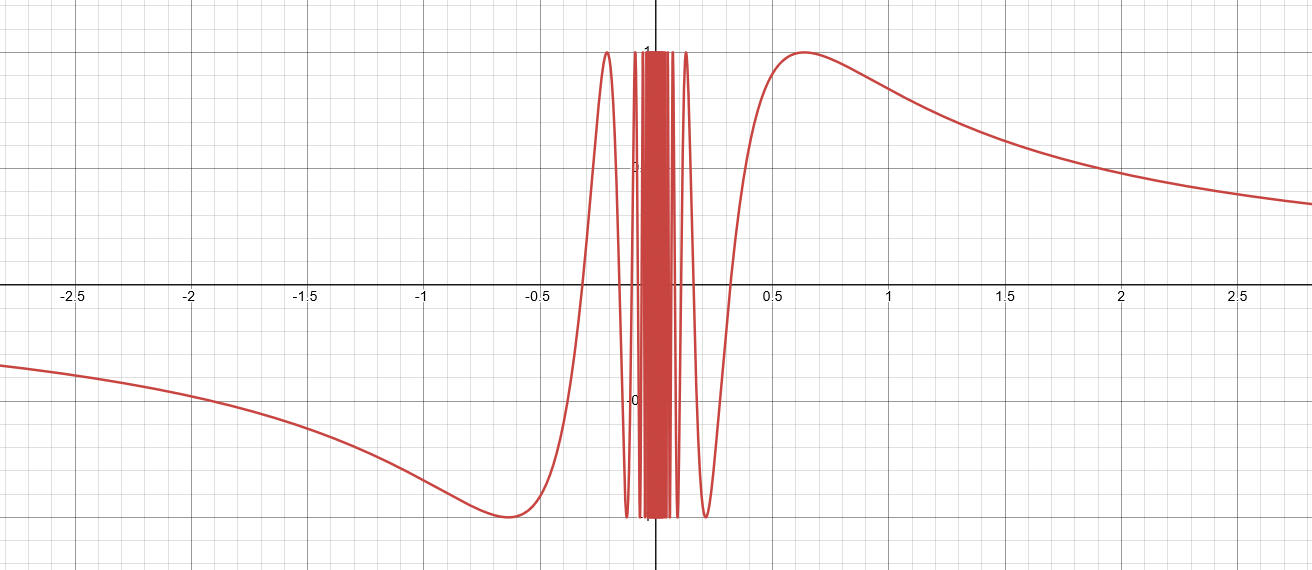
\includegraphics[width=\textwidth]{img/lecture13/graph_of_sin}
		\end{center}
	\end{explanation}
	
	\section{Разрывы монотонной функции}
	
	\begin{sentence}
		Пусть $f$ - монотонная на интервале $(a, b)$ функция (т. е. $f$ либо не убывает, либо не возрастает). Тогда $f$ может иметь разрывы только первого рода на интервале $(a, b)$.
	\end{sentence}
	
	\begin{proof}
		Сначала оговоримся, что когда говорят о функции монотонной на $(a, b)$, подразумевают, что она определена в каждой точке на этом интервале.
		
		Пусть $x_0$ - точка разрыва, $x_0 \in (a, b) \Rightarrow x_0$ - предельная для множества $D^-_{x_0}$ и $D^+_{x_0}$. Будем считать, что $f(x)$ не убывает (без ограничения общности) $\Rightarrow$ по теореме Вейерштрасса 
		\[ \exists \lim_{x \to x_0+} f(x) = \sup_{x < x_0} f(x) \leqslant f(x_0) \text{ } (f \text{ не убывает}) \]
		Тоже самое для правой окрестности:
		\[ \exists \lim_{x \to x_0+} f(x) = \inf_{x > x_0} f(x) \geqslant f(x_0) \]
		Тогда $\lim_{x \to x_0-} f(x) \leqslant f(x_0) \leqslant \lim_{x \to x_0+} f(x).$
		
		Это не разрыв 2-го рода, т. к. пределы справа и слева существует. Если бы это был разрыв устранимый, то пределы справа и слева совпадают, но тогда $\lim_{x \to x_0} f(x) = f(x_0) \Rightarrow$ это не является разрывом. Значит если точка $x_0$ является разрывом $\Rightarrow$ скачок ненулевой $\Rightarrow$ это разрыв 1-го рода.
		
		Применяя теорему Вейерштрасса, мы пользовались тем, что $f(x)$ ограничена на интервале $(a, b)$. Пусть это не так.
		
		\begin{center}
			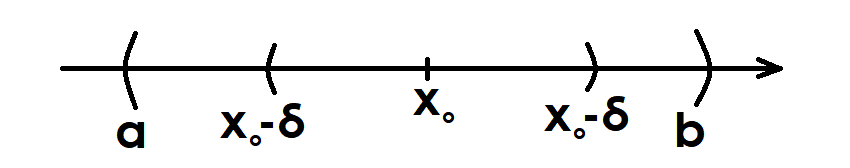
\includegraphics[width=0.5\textwidth]{img/lecture13/interval_line}
		\end{center}
		
		Тогда рассмотрим $\delta$-окрестность точки $x_0$. $x_0 - \delta$ и $x_0 + \delta$ лежат внутри $(a, b) \Rightarrow$ функция определена в этих точках $\Rightarrow \exists f(x_0 - \delta)$ и $\exists f(x_0 + \delta) \Rightarrow f(x_0 - \delta) \leqslant f(x) \leqslant f(x_0 + \delta).$ Т. е. на всём интервале $(a, b)$ функция может быть неограничена, но на интервале $(x_0 - \delta, x_0 + \delta)$ она ограничена и здесь значения функции определены. Поэтому мы пользуемся теоремой Вейерштрасса не на всём интервале $(a, b)$, а на подинтервале $(x_0 - \delta, x_0 + \delta)$.
	\end{proof}
	
	\section{Теорема Вейерштрасса}
	
	\begin{definition}
		Функцию, непрерывную в каждой точке множества $D$ (по множеству $D$), будем называть просто непрерывной на множестве $D$.
		
		Краткая запись: $f(x) \in C(D)$ - функция непрерывна на множестве $D$.
	\end{definition}
	
	\begin{definition}
		Будем говорить, что функция ограничена на множестве $D$, если найдется такое число $C > 0$, что $\forall x \in [a, b] \rightarrow |f(x)| \leqslant C$.
	\end{definition}
	
	\begin{theorem}[Вейерштрасс]
		Пусть функция $f$ непрерывна на отрезке $[a, b]$. Тогда она ограничена на $[a, b]$ и достигает минимума и максимума, т. е. существуют такие точки $x_m, x_M \in [a, b]$, что
		\[ f(x_m) = \inf\{f(x) : x \in [a, b]\} \text{ и } f(x_M) = \sup\{f(x) : x \in [a, b]\}. \]
	\end{theorem}
	
	\begin{proof}
		\begin{enumerate}
			\item $f(x)$ - ограничена.
			
			Пусть это не так:
			\[ \forall n \geqslant \N \text{ } \exists x_n \in [a, b]: |f(x_n)| > n \text{ } (*) \]
			Все такие $\{x_n\}$ образуют ограниченную последовательность, т. к. все $x_n \in [a, b] \Rightarrow$ можно выделить $\{x_{n_k}\}$ - сходящуюся подпоследовательность, пусть $x_{n_k} \to x_0.$ Тогда $f(x_{n_k}) \to f(x_0),$ т. к. $f(x)$ - непрерывна (предложение 4.4). Но такого не может быть, т. к. $|f(x_{n_k})| > n_k$ (пользуемся (*)), а $n_k \to \infty$.
			\item Докажем, что $\sup_{x \in [a, b]} f(x) = M$ и $\inf_{x \in [a, b]} f(x) = m$ достигаются.
			
			Докажем следующие $x_n$: $M - \frac{1}{n} \leqslant f(x_n) \leqslant M$ (**). Такие $x_n$ (их бесконечно много) найдутся из определения супремума. Значит $x_n$ - ограниченная последовательность $\Rightarrow \exists x_{n_k}$ - подпоследовательность, сходящаяся к $x_M \Rightarrow \exists \lim_{n_k \to \infty} f(x_{n_k}) = f(x_M)$ (по непрерывности функции) и с другой стороны $\lim_{n_k \to \infty} f(x_{n_k}) = M$ (по теореме о зажатой последовательности, применяемой к (**)). Следовательно, $f(x_M) = M$.  
		\end{enumerate}
	\end{proof}
	
	\section{Теорема о промежуточном значении}
	
	\begin{theorem}[Коши]
		Пусть $f$ непрерывна на отрезке $[a, b]$. Если $f(a) = A, f(b) = B$, то для каждого значения $C \in [A, B]$ (или $C \in [B, A]$, если $B < A$) найдется точка $c \in [a, b]$, для которой $f(c) = C$.
	\end{theorem}
	
	\begin{center}
		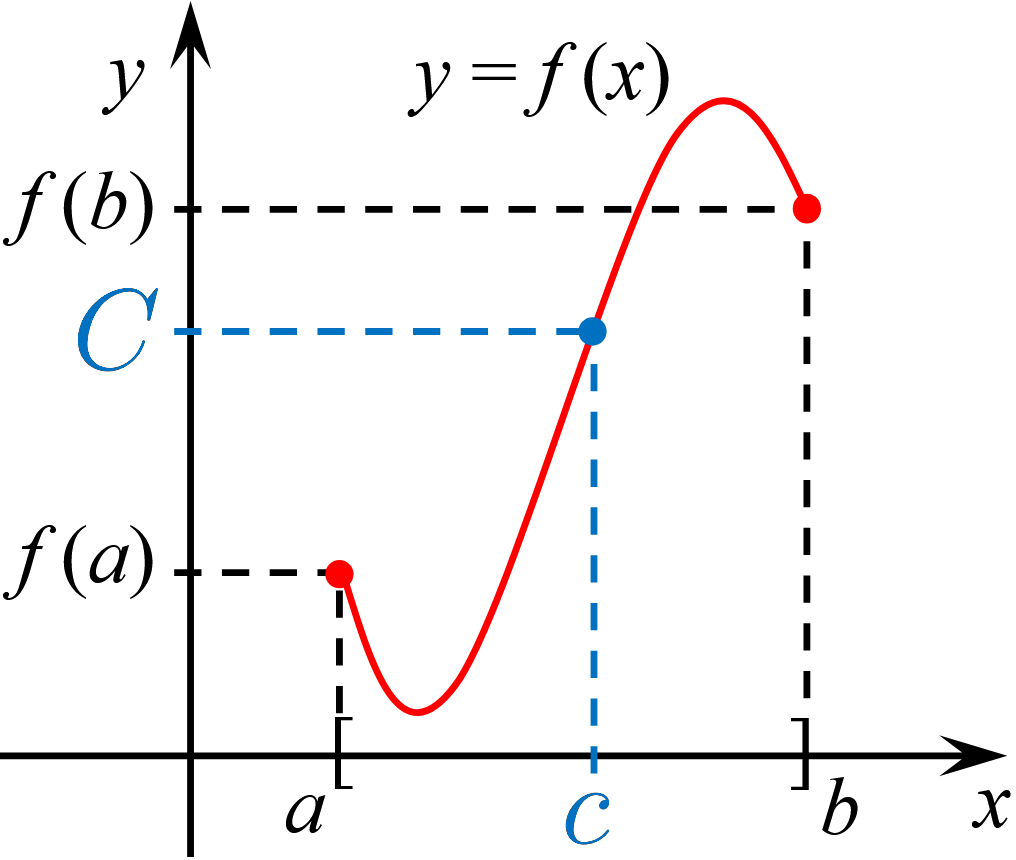
\includegraphics[width=0.5\textwidth]{img/lecture13/intermediate_value_theorem}
	\end{center}
	
	\begin{proof}
		\begin{enumerate}
			\item $g(x) = f(x) - C,$ т. е. хотим доказать, что $\exists c: g(x) = 0.$
			\item Если $g(a) = 0$, то $c = a$. Если $g(b) = 0$, то $c = b$. Поэтому будем считать, что $g(a) \neq 0$ и $g(b) \neq 0$. Но тогда  $g(a)$ и $g(b)$ разного знака, т. к. $A \leqslant C \leqslant B$ или $B \leqslant C \leqslant A$.
			\item Рассмотрим отрезок $[a, b]$ и точку $\frac{a + b}{2}$.
			
			Если $g\big(\frac{a + b}{2}\big) = 0,$ то мы нашли такую точку, что $g(x) = 0$.
			
			Если $g\big(\frac{a + b}{2}\big) > 0,$ то рассматриваем отрезок $[a; \frac{a + b}{2}]$.
			
			Если $g\big(\frac{a + b}{2}\big) < 0,$ то рассматриваем отрезок $[\frac{a + b}{2}; b]$.
			
			(Таким образом, мы зажимаем искомую точку отрезком, в одном конце которого $g(x) < 0$, а в другом $g(x) > 0$)
			
			Если ни одной точки, где $g(c) = 0$ не найдено, то мы получим последовательность вложенных отрезков. Тогда по теореме о вложенных отрезков $\exists c \in [a, b]$ - общая точка (длина отрезков стремится к нулю, потому что мы каждый раз длину делим пополам, $\frac{b - a}{2^n} \to 0$)
			
			Левые концы отрезков обозначим $a_n$, правые - $b_n$. Тогда $\lim_{n \to \infty} a_n = c, \lim_{n \to \infty} b_n = c$. Из непрерывности функции следует, что $\lim_{n \to \infty} g(a_n) = g(c) \leqslant 0$ (т. к. $g(a_n) < 0$) и $\lim_{n \to \infty} g(b_n) = g(c) \geqslant 0$ (т. к. $g(b_n) > 0$) $\Rightarrow 0 \leqslant g(c) \leqslant 0 \Rightarrow g(c) = 0 \Rightarrow f(c) = C.$
			
		\end{enumerate}
	\end{proof}
	
	\newpage
	
	\section*{Лекция 14: Построение показательной функции}
	
	\begin{theorem}[Критерий непрерывности монотонной функции]
		Монотонная функция $f : [a, b] \to \R$ непрерывна на $[a, b]$ тогда и только тогда, когда $f([a, b])$ - отрезок ($f([a, b]) = \{f(x) | x \in [a, b]\}$ - образ).
	\end{theorem}
	
	\begin{proof}
	    Будем считать, что $f$ - не убывает без ограничения общности.
	    \begin{itemize}
	    	\item[$\Rightarrow$]
		    \begin{enumerate}
		    	\item По теореме Коши $\forall C \in [f(a), f(b)]$ $\exists c \in [a, b]: f(c) = C,$ т. к. $f$ - непрерывна на $[a, b]$.
		    	\item $\forall x \in [a, b]$ $f(a) \leqslant f(x) \leqslant f(b)$ (функция монотонная)
		    	
		    	2 пункт утверждает, что образ $f([a, b])$ содержится в отрезке $[f(a), f(b)]$, т. е. все точки образа лежат в $[f(a), f(b)]$. И при этом они лежат плотно друг к другу (т. е. нет дырок, иначе это не был бы отрезок), это следует из 1 пункта.
		    \end{enumerate}
		    \item[$\Leftarrow$] $f([a, b]) = [f(a), f(b)]$ (из того, что $f$ - не убывает, следует, что $f(a)$ - левая граница отрезка, а $f(b)$ - правая граница отрезка).
		    
		    Пусть $f$ - не непрерывна $\Rightarrow$ у неё есть точки разрыва. Пусть $x_0$ - точка разрыва $\Rightarrow$ из предложения 4.11 (т. к. $f$ - монотонна) $x_0$ - разрыв 1-го рода $\Rightarrow \exists \lim_{x \to x_0-} f(x) = \sup_{x < x_0} f(x)$ и $\exists \lim_{x \to x_0+} f(x) = \inf_{x > x_0} f(x)$ (как в предложении 4.11) и эти пределы не равны $\Rightarrow (\sup_{x < x_0} f(x), \inf_{x > x_9} f(x))$ - не пустой. Тогда этом интервале есть точка $C \neq f(x_0) \Rightarrow \not\exists c: f(c) = C.$
		    
		    \begin{center}
		    	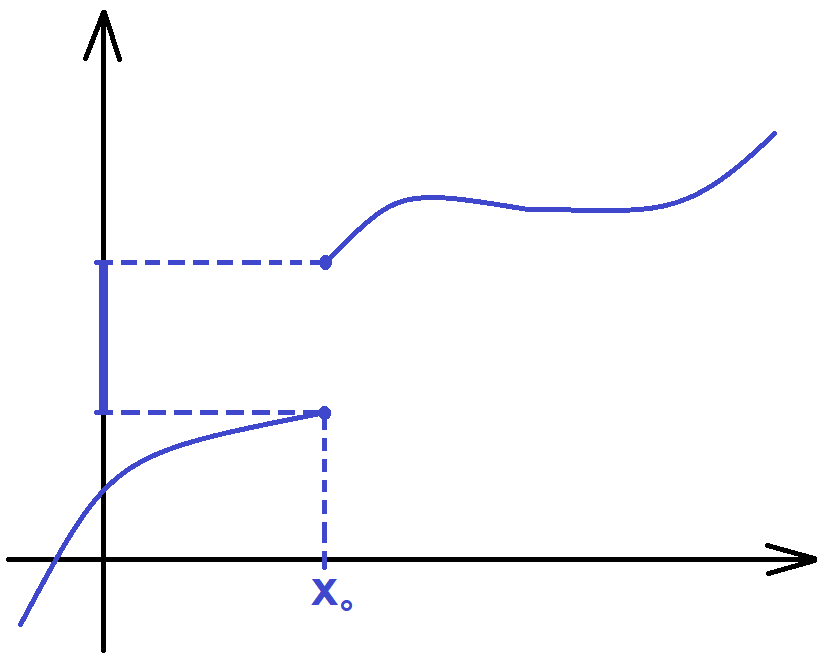
\includegraphics[width=0.3\textwidth]{img/lecture14/graph_of_monotonic _function}
		    \end{center}
		    
		    \begin{tabular}{cc|c}
		    	Иначе & $\sup_{x < x_0} f(x) < C = f(c) \Rightarrow c \geqslant x_0$ & \multirow{2}*{$\Rightarrow c = x_0$, но $f(x_0) \neq C$.} \\
		    	& $\inf_{x > x_0} f(x) > C = f(c) \Rightarrow c \leqslant x_0$ &
		    \end{tabular}
		    
		    Если $x_0 = a$, то рассмотрим интервал $(\sup_{x < x_0} f(x), f(x_0))$, если $x_0 = b$, то рассмотрим интервал $(f(x_0), \inf_{x > x_0} f(x))$.
		\end{itemize}
	\end{proof}
	
	\section{Непрерывность обратной функции}
	
	\begin{theorem}[О непрерывности обратной функции]
		Пусть $f$ непрерывна и строго монотонна на $[a, b]$ (т. е. $f$ монотонна и $f(x) \neq f(y)$ при $x \neq y$). Тогда $f$ - биекция между отрезками $I = [a, b]$ и $J$ с концами $f(a)$ и $f(b)$ и $f^{-1}$ непрерывна и строго монотонна на $J$.
	\end{theorem}
	
	\begin{proof}
		$f$ - строго возрастает (без ограничения общности).
		\begin{enumerate}
			\item $f$ - инъекция. $\newline$
			\begin{tabular}{c|c}
				$x_1 < x_2 \Rightarrow f(x_1) < f(x_2)$ & \multirow{2}*{$\Leftrightarrow (x_1 \neq x_2 \Rightarrow f(x_1) \neq f(x_2))$} \\
				$x_1 > x_2 \Rightarrow f(x_1) > f(x_2)$ &
			\end{tabular}
			\item $f$ - сюръекция.
			
			$f$ - непрерывная, монотонная $\Rightarrow$ по теореме 4.16 $f([a, b]) = [f(a), f(b)]$ для любой точки отрезка есть прообраз.
			
			Из 1) и 2) $f$ - биекция $\Rightarrow \exists f^{-1}(y)$.
			\item $f^{-1}(y)$ - монотонная.
			
			Пусть $y_1 < y_2 (y_1, y_2 \in [f(a), f(b)]), y_1 = f(x_1), y_2 = f(x_2) \Rightarrow f(x_1) < f(x_2) \Rightarrow x_1 < x_2$.
			
			$x_1 = f^{-1}(y_1), x_2 = f^{-1}(y_2), x_1 < x_2 \Rightarrow f^{-1}(y_1) < f^{-1}(y_2)$
			
			В итоге: $y_1 < y_2 \Rightarrow f^{-1}(y_1) < f^{-1}(y_2)$.
			\item $f: I \rightarrow J \Rightarrow f^{-1}: J \rightarrow I$ (функция из отрезка в отрезок) $\Rightarrow$ по теореме 4.16 $f^{-1}$ - непрерывная.
		\end{enumerate}
	\end{proof}
	
	\begin{example}
		У функции $f(x) = \tg{x}$ на интервале $\big(-\frac{\pi}{2}, \frac{\pi}{2})$ есть непрерывная и строго монотонная на $\R$ обратная функция.
	\end{example}
	
	\begin{proof}
		Функцию $f(x) = \tg{x}$ строго возрастает и непрерывна на интервале $\big(-\frac{\pi}{2}, \frac{\pi}{2}\big)$. Поэтому образ отрезка $\big[-\frac{\pi}{2} + \frac{1}{n}, \frac{\pi}{2} - \frac{1}{n}\big]$ есть отрезок 
		
		$\big[\tg{\big(-\frac{\pi}{2} + \frac{1}{n}\big)}, \tg{\big(\frac{\pi}{2} - \frac{1}{n}\big)}\big]$, на котором существует непрерывная строго монотонная обратная функция $f^{-1}_n$ (теорема 4.17). Эти функции согласованы, т. е. $f^{-1}_{n + 1}(x) = f^{-1}_n(x)$ для каждой точки 
		\[ x \in \bigg[\tg{\bigg(-\frac{\pi}{2} + \frac{1}{n}\bigg)}, \tg{\bigg(\frac{\pi}{2} - \frac{1}{n}\bigg)}\bigg], \text{ a } \bigcup_{n = 1}^{\infty} \bigg[\tg{\bigg(-\frac{\pi}{2} + \frac{1}{n}\bigg)}, \tg{\bigg(\frac{\pi}{2} - \frac{1}{n}\bigg)}\bigg] = \R. \]
		$(\tg{\big(-\frac{\pi}{2} + \frac{1}{n}\big)} \to -\infty, \tg{\big(\frac{\pi}{2} - \frac{1}{n}\big)}) \to +\infty$
		
		Тем самым, построена обратная функция $f^{-1}$ на $\R$, которую мы обозначим $\arctg{x}$.
	\end{proof}
	
	\section{Построение показательной функции}
	
	Пусть $a > 1$. Будем считать известным из школьного курса, что для рациональных $x$ значение $a^x$ корректно определено и выполнены свойства
	\[ a^0 = 1, a^{x + y} = a^x \cdot a^y, x < y \Rightarrow a^x < a^y \]	
	для рациональных $x$ и $y$.
	
	\begin{lemma}
		Пусть $N \in \N$. Тогда найдется такое число $C(N)$, что для всех $x, y \in \Q, x, y \leqslant N$, выполнено $|a^x - a^y| \leqslant C(N)|x - y|$
	\end{lemma}
	
	\begin{proof}
		Если $x - y \geqslant 1$, то $0 < a^x - a^y \leqslant a^x \leqslant a^N \leqslant a^N|x - y| = C(N)|x - y|$.
		
		Если $0 < |x - y| < 1$, то найдётся натуральное число $n$, для которого $\frac{1}{n + 1} \leqslant x - y < \frac{1}{n}$. Тогда
		\[ a^x - a^y = a^y(a^{x - y} - 1) \leqslant a^N(a^{x - y} - 1) \leqslant a^N(a^{\frac{1}{n}} - 1) \leqslant a^N \frac{(a - 1)}{n} \]
		\begin{explanation}
			Докажем последнее неравенство
			
			$(a^{\frac{1}{n}} - 1) \leqslant \frac{a - 1}{n} \Leftrightarrow n(a^{\frac{1}{n}} - 1) \leqslant a - 1 \Leftrightarrow n(a^{\frac{1}{n}} - 1) + 1 \leqslant a$
			
			$x = a^{\frac{1}{n}} - 1 > 0 \Leftrightarrow x + 1 = a^{\frac{1}{n}} \Leftrightarrow (x + 1)^n = a$
			
			Из последних двух строчек следует неравенство Бернулли: $nx + 1 \leqslant (x + 1)^n$. Повторяем шаги в обратную сторону и доказываем требуемое неравенство.
		\end{explanation}
		\[ \frac{1}{n} \leqslant \frac{2}{n + 1} \Rightarrow a^N \frac{(a - 1)}{n} \leqslant \frac{2a^N(a - 1)}{n + 1} \]
		\[ \frac{1}{n + 1} \leqslant x - y \Rightarrow \frac{2a^N(a - 1)}{n + 1} \leqslant 2a^N(a - 1)(x - y) = C(N)(x - y) \]
		\[ C(N) = \max\{a^N, 2a^N(a - 1)\} \]
	\end{proof}
	
	\newpage
	
	\section*{Лекция 15: Производная и дифференциал}
	
	\begin{theorem}
		Пусть $a > 1$. Существует единственная непрерывная функция $f : \R \rightarrow \R$, совпадающая с $x \mapsto a^x$ при $x \in \Q$.
	\end{theorem}
	
	\begin{proof}
	\end{proof}
	
	\begin{corollary}
		Для построенной функции $a^x$ выполнены следующие свойства:
		\[ a^{x + y} = a^x \cdot a^y \text{ и } x < y \Rightarrow a^x < a^y. \]
	\end{corollary}
	
	\begin{proof}
	\end{proof}
	
	По теореме об обратной функции корректно определена
	непрерывная строго монотонная функция $\log_a : (0, +\infty) \rightarrow \R$.
	
	\chapter{Производная}
	
	\section*{Лекция 16: Свойства дифференцируемых функций}
	
	\section*{Лекция 17: Теоремы о среднем для дифференцируемых функций}
	
	\section*{Лекция 18: Правило Лопиталя, производные старших порядков}
	
	\section*{Лекция 19: Формула Тейлора}
	
	\section*{Лекция 20: Ряд Тейлора}
	
	\chapter{Исследование функций с помощью производных}
	
	\section*{Лекция 21: Исследование функций с помощью производных}
	
	\section{Необходимое условие экстремума}
	
	Напомним, что для дифференцируемой в точке локального экстремума $c$ функции $f$ по теореме Ферма выполнено $f'(c) = 0$. Т. е. равенство нулю производной является необходимым условием локального экстремума дифференцируемой функции. 
	
	Напомним, что нами также было уже доказано следствие 5.26:
	
	\textbf{Следствие (5.26)} Пусть $f$ дифференцируема в каждой точке интервала $(a, b)$. Тогда $f$ не
	убывает (не возрастает) на $(a, b)$ тогда и только тогда, когда $f'(x) \geqslant 0 \text{ } (f'(x) \leqslant 0$ соответственно) для каждой точки $x \in (a, b)$. Кроме того, если $f'(x) > 0 \text{ } (f'(x) < 0)$, то $f$ строго возрастает (соответственно, строго убывает) на $(a, b)$.
	
	Докажем теперь достаточное условие локального экстремума в терминах производных старших порядков.
	
	\section{Достаточное условие экстремума}

	
	\begin{theorem}
		Пусть $f$ имеет n производных в окрестности точки $c \in (a, b)$ и $f(c) = f'(c) = ... = f^{(n - 1)}(c) = 0$, а $f^{(n)}(c) \neq 0$. Тогда, если $n = 2k$ и $f^{(n)}(c) < 0 \text{ } (f^{(n)}(c) > 0)$, то $c$ — точка локального максимума (минимума). Если $n = 2k + 1$, то точка c не является точкой локального экстремума.
	\end{theorem}
	
	\begin{proof}
		По формуле Тейлора
		\[ f(x) = f(c) + \frac{f'(c)}{1!} \cdot (x - c) + ... + \frac{f^{(n - 1)}(c)}{(n - 1)!}(x - c)^{n - 1} + \frac{f^{(n)}(c)}{n!}(x - c)^n + o((x - c)^n) = \]
		\[ = \frac{f^{(n)}(c)}{n!}(x - c)^n + o((x - c)^n) = (x - c)^n \bigg(\frac{f^{(n)}(c)}{n!} + o(1)\bigg) \]
		Т. к. $o(1) \to 0$ при $x \to c$, то по определению предела
		\[ \exists B_{\delta}(c): \forall x \in B_{\delta}(c) \rightarrow |o(1)| < \epsilon = \bigg|\frac{f^{(n)}{(c)}}{n!}\bigg| \Rightarrow \]
		$\Rightarrow \forall x \in B_{\delta}(c)$ $\big(\frac{f^{(n)}(c)}{n!} + o(1)\big)$ имеет тот же знак, что и $f^{(n)}(c)$
		\begin{enumerate}
			\item Если $n = 2k$ и $f^{(n)}(c) > 0$, то $f(x) = (x - c)^n \big(\frac{f^{(n)}(c)}{n!} + o(1)\big) = (x - c)^{2k} \cdot A(x)$ $(A(x) > 0$ $\forall x \in B_{\delta}(c))$
			
			При $x = c$ $f(c) = 0$; так только мы отходим от точки $c$, $f(x) > 0 \Rightarrow c$ - точка минимума.
			\item Если $n = 2k$ и $f^{(n)}(c) < 0$, то $f(x) = (x - c)^n \big(\frac{f^{(n)}(c)}{n!} + o(1)\big) = (x - c)^{2k} \cdot A(x)$ $(A(x) < 0$ $\forall x \in B_{\delta}(c))$
			
			При $x = c$ $f(c) = 0$; так только мы отходим от точки $c$, $f(x) < 0 \Rightarrow c$ - точка максимума.
			\item Если $n = 2k + 1$ и $f^{(n)}(c) > 0$, то $f(x) = (x - c)^n \big(\frac{f^{(n)}(c)}{n!} + o(1)\big) = (x - c)^{2k + 1} \cdot A(x)$ $(A(x) > 0$ $\forall x \in B_{\delta}(c))$
			
			При $x = c$ $f(c) = 0$; так только мы отходим от точки $c$ в положительную сторону, $f(x) > 0$; так только мы отходим от точки $c$ в отрицательную сторону, $f(x) < 0 \Rightarrow c$ - ни точка максимума, ни точка минимума.
			\item Если $n = 2k + 1$ и $f^{(n)}(c) < 0$, то $f(x) = (x - c)^n \big(\frac{f^{(n)}(c)}{n!} + o(1)\big) = (x - c)^{2k + 1} \cdot A(x)$ $(A(x) < 0$ $\forall x \in B_{\delta}(c))$
			
			При $x = c$ $f(c) = 0$; так только мы отходим от точки $c$ в положительную сторону, $f(x) < 0$; так только мы отходим от точки $c$ в отрицательную сторону, $f(x) > 0 \Rightarrow c$ - ни точка максимума, ни точка минимума.
		\end{enumerate}
		
		Хочется отметить, что выполнение условия теоремы $f(c) = f'(c) = ... = f^{(n - 1)}(c) = 0$ можно гарантировать, сдвинув функцию на константу: $g(x) = f(x) - f(c)$.
	\end{proof}
	
	\section{Выпуклость и вогнутость}
	
	\begin{definition}
		Функция $f$ на интервале $(a, b)$ называется \textbf{выпуклой}, если $\forall x, y \in (a, b)$ и для каждого $t \in [0, 1]$ выполнено
		\[ f(tx + (1 - t)y) \leqslant tf(x) + (1 - t) f(y). \]
	\end{definition}
	
	\begin{explanation}
	    Функция $tx + (1 - t)y$ при фиксированных $x$ и $y$	при различных значениях $t \in [0, 1]$ задаёт точку на отрезке $[x, y]$: при $t = 0$ функция равна $y$, при $t = 1$ функция равна $x$, если возьмём производную функции $tx + (1 - t)y$, то получим $x - y < 0 \Rightarrow$ функция монотонно убывает от $y$ до $x$.
	    
	    Функция $t f(x) + (1 - t) f(y)$ от $t$ является линейной и она задаёт хорду c концами в точках $(x, f(x))$ (при $t = 1$) и $(y, f(y))$ (при $t = 0$). 
	    
	    Получается с левой стороны неравенства - это значение функции в точке на отрезке $[x, y]$, а с правой - ордината точки на хорде и понятно, что неравенство выполняется.
	\end{explanation}
	
	\begin{center}
		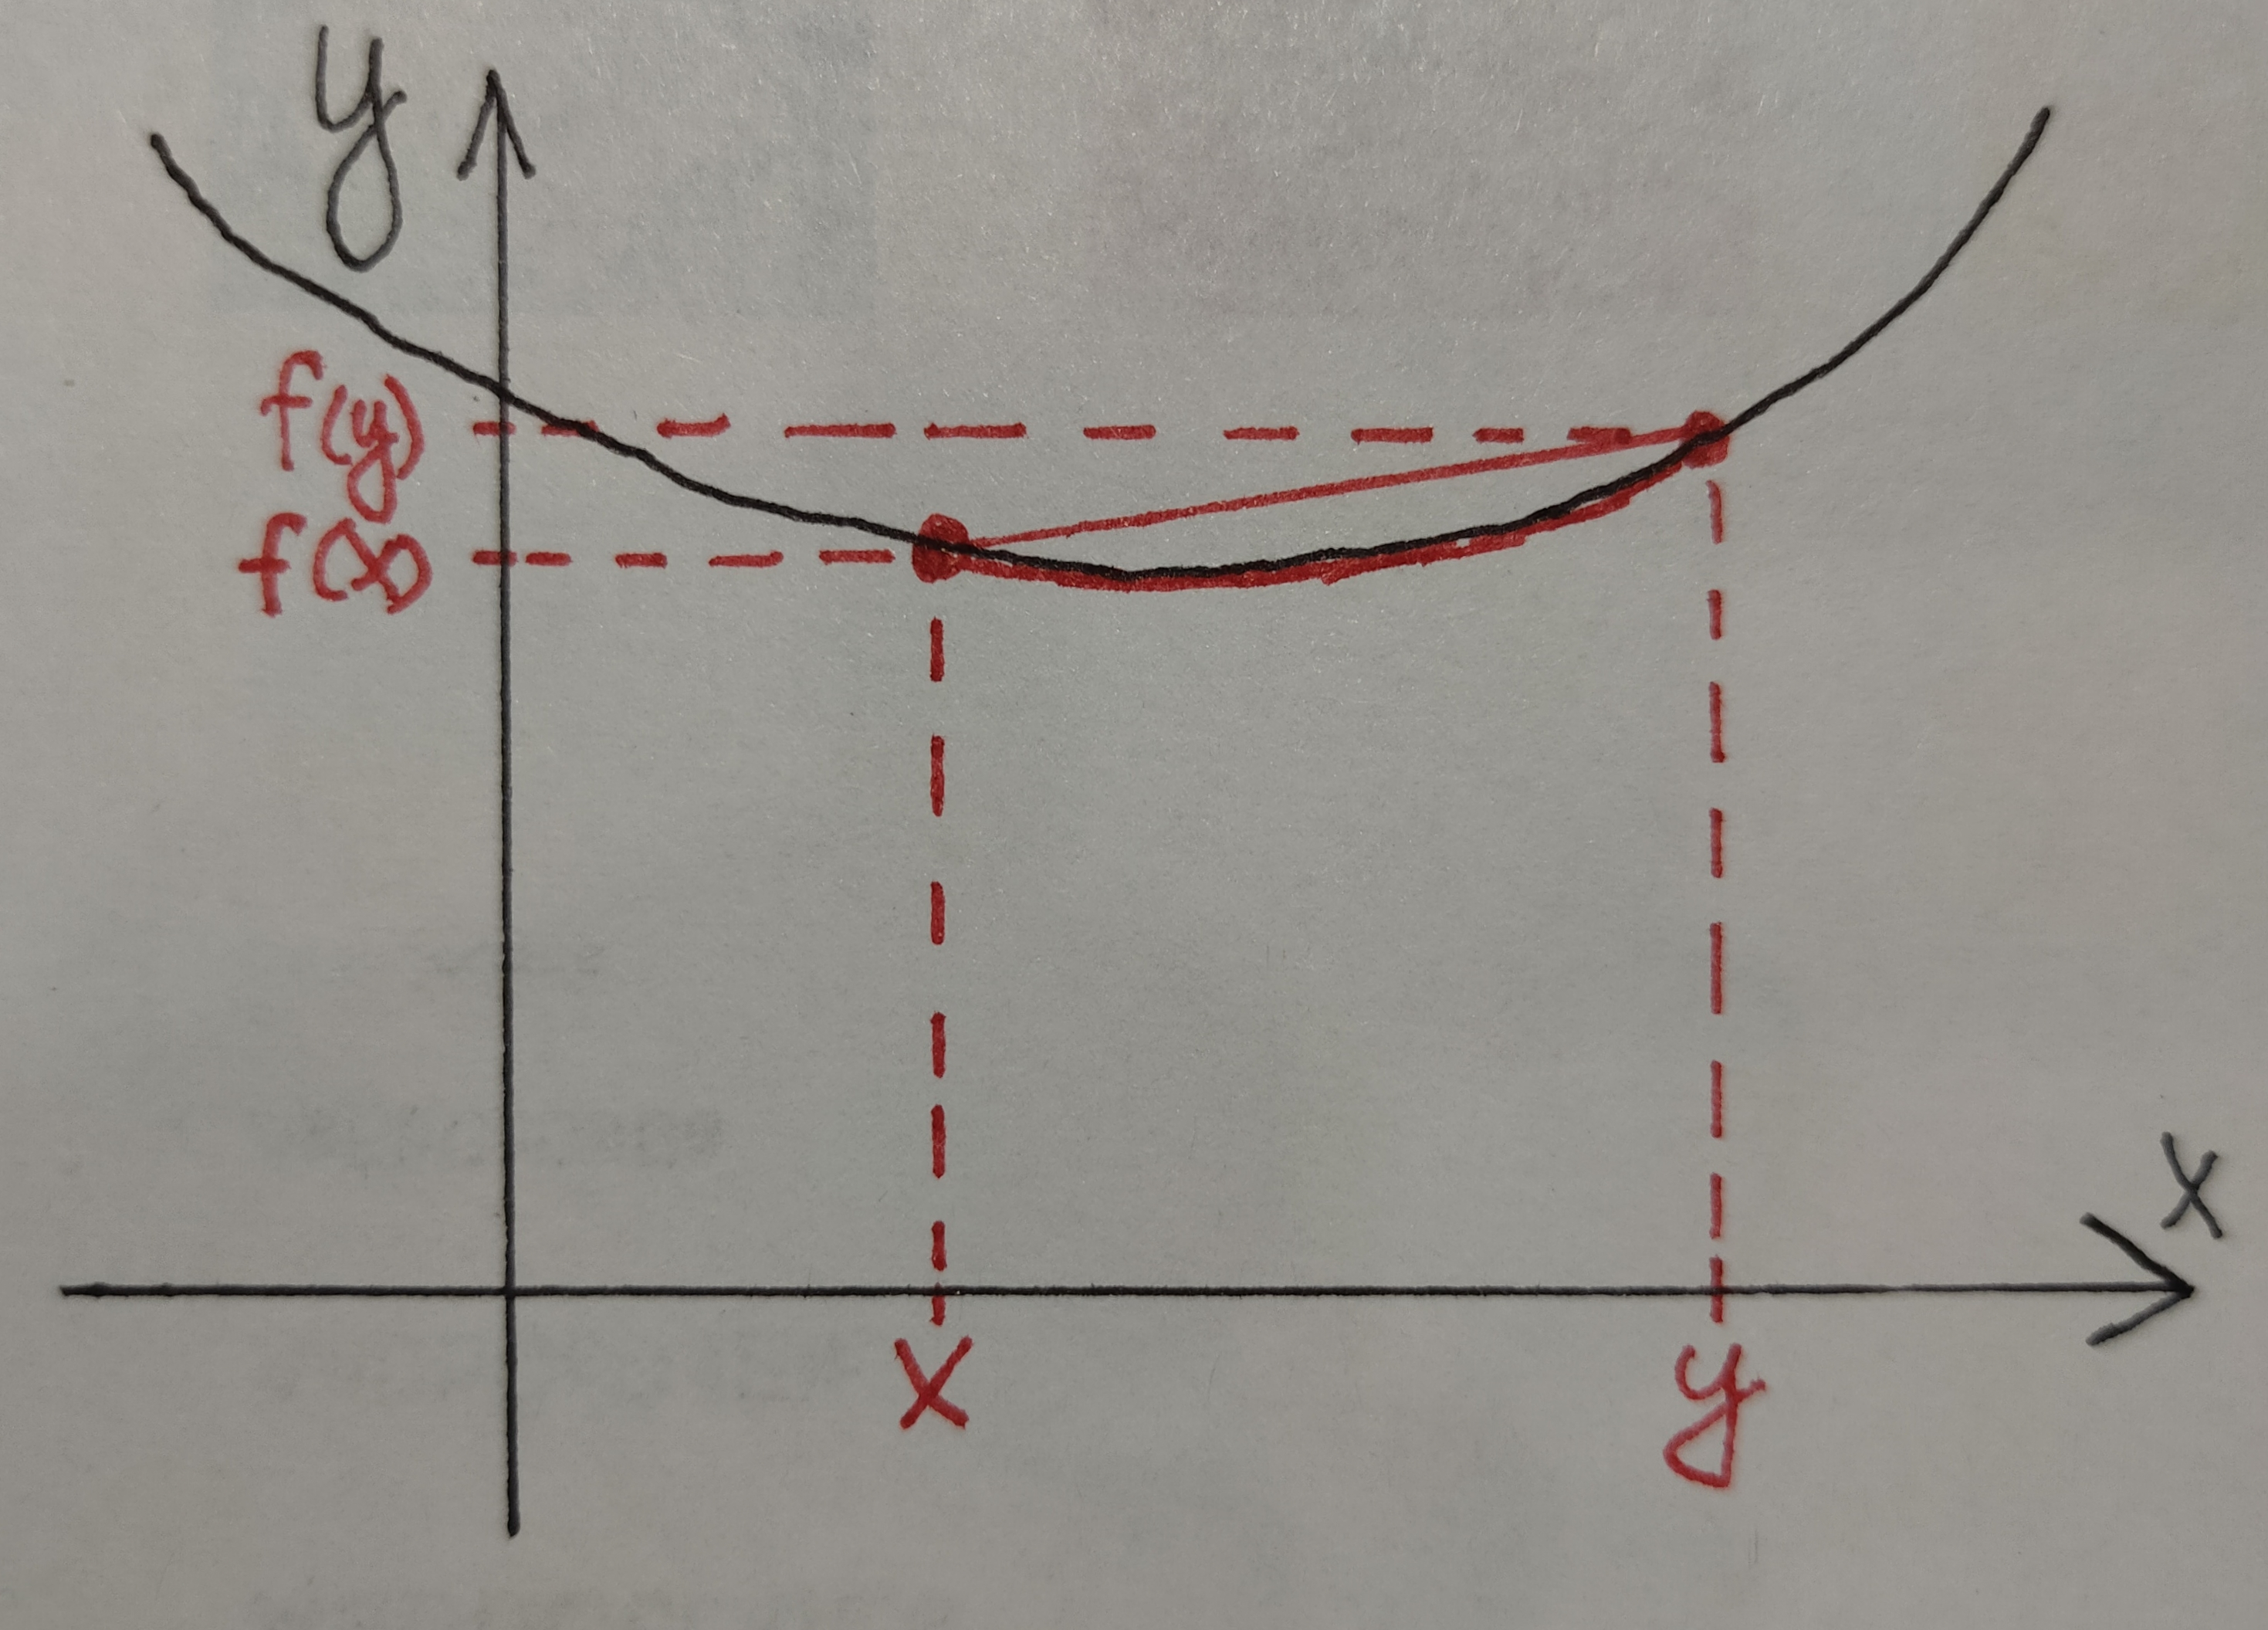
\includegraphics[width=0.4\textwidth]{img/lecture21/convex}
	\end{center}
	
	\begin{definition}
		Функция $f$ на интервале $(a, b)$ называется \textbf{вогнутой}, если $\forall x, y \in (a, b)$ и для каждого $t \in [0, 1]$ выполнено
		\[ f(tx + (1 - t)y) \geqslant tf(x) + (1 - t)f(y). \]
	\end{definition}
	
	\begin{lemma}
		Функция $f$ на интервале $(a, b)$ выпукла тогда и только тогда, когда для всех точек $x < z < y$ из этого интервала выполнено
		\[ \frac{f(z) - f(x)}{z - x} \leqslant \frac{f(y) - f(z)}{y - z} \]
	\end{lemma}
	
	\begin{proof}
		Неравенство, которое нужно доказать эквивалентно
		\[ \frac{f(z) - f(x)}{z - x} \leqslant \frac{f(y) - f(z)}{y - z} \text{ } \bigg| \cdot (z - x)(y - z) \]
		\[ yf(z) - zf(z) - yf(x) + zf(x) \leqslant zf(y) - xf(y) - zf(z) + xf(z) \]
		\[ xf(z) - yf(z) \geqslant zf(x) - yf(x) + xf(y) - zf(y) \]
		
		Т. к. $x < z < y$, то $\exists t \in [0, 1]$ $z = t \cdot x + (1 - t) \cdot y \Leftrightarrow t = \frac{z - y}{x - y}$.
		
		Т. к. $f(x)$ - выпукла, то $f(z) = f(t \cdot x + (1 - t) \cdot y) \leqslant t f(x) + (1 - t) f(y) = \frac{z - y}{x - y} f(x) + \frac{x - z}{x - y} f(y) \Leftrightarrow xf(z) - yf(z) \geqslant zf(x) - yf(x) + xf(y) - zf(y)$, т. е пришли к тому же самому неравенству.
		
		В обратную сторону.	Имеем, что
		\[ \frac{f(z) - f(x)}{z - x} \leqslant \frac{f(y) - f(z)}{y - z} \Rightarrow xf(z) - yf(z) \geqslant zf(x) - yf(x) + xf(y) - zf(y) \Rightarrow \]
		\[ \Rightarrow f(z) \leqslant \frac{z - y}{x - y} f(x) + \frac{x - z}{x - y} f(y) \]
		Т. к. $x < z < y$, то $\exists t \in [0, 1]$ $z = t \cdot x + (1 - t) \cdot y \Leftrightarrow t = \frac{z - y}{x - y}$.
		
		Значит
		\[  f(t \cdot x + (1 - t) \cdot y) \leqslant t f(x) + (1 - t) f(y), \]
		что является определением выпуклости функции.
	\end{proof}
	
	\begin{theorem}
		Дифференцируемая функция $f$ на интервале $(a, b)$ выпукла тогда и только тогда, когда $f'$ — неубывает.
	\end{theorem}
	
	\begin{proof}
		\begin{enumerate}
			\item[$\Rightarrow$] $\forall x < z < y \in (a, b)$
			$f$ - выпукла $\Rightarrow$ по предыдущей лемме
			\[ \frac{f(z) - f(x)}{z - x} \leqslant \frac{f(y) - f(z)}{y - z} \]
			Тогда при $z \to x$ по теореме о переходе к пределу в неравенстве
			\[ f'(x) \leqslant \frac{f(y) - f(x)}{y - x} \]
			(Здесь есть тонкость: мы можем устремлять $z$ к $x$ только справа, поэтому мы получим правую производную, но если функция дифференцируема, то правая производная совпадает с левой)
			
			Пусть $z \to y$. Тогда
			\[ \frac{f(y) - f(x)}{y - x} \leqslant f'(y) \]
		    Таким образом, $\forall x < y$ $f'(x) \leqslant f'(y) \Rightarrow f'(x)$ - неубывает. 
			\item[$\Leftarrow$] Пусть $x < z < y$
			
			По теореме Лагранжа $\exists \xi_1 \in (x, z): \frac{f(z) - f(x)}{z - x} = f'(\xi_1)$
			
			$\exists \xi_2 \in (z, y): \frac{f(y) - f(z)}{y - z} = f'(\xi_2)$
			
			Таким образом, $\xi_1 \leqslant \xi_2 \Rightarrow f'(\xi_1) \leqslant f'(\xi_2) \Rightarrow \frac{f(z) - f(x)}{z - x} \leqslant \frac{f(y) - f(z)}{y - z} \Rightarrow f$ на интервале $(a, b)$ выпукла по предыдущей лемме.
		\end{enumerate}
	\end{proof}
	
	\begin{corollary}
		Дважды дифференцируемая функция $f$ на интервале $(a, b)$ выпукла тогда и только тогда, когда $f''(x) \geqslant 0 \text{ } \forall x \in (a, b).$
	\end{corollary}
	
	\begin{proof}
		$f''(x) \geqslant 0 \Leftrightarrow f'(x)$ неубывает. 
	\end{proof}
	
	\begin{corollary}
		Пусть $f$ — дифференцируемая выпуклая функция на интервале $(a, b)$. Тогда $f(x) \geqslant f'(c)(x - c) + f(c)$ для всех $x, c \in (a, b)$.
    \end{corollary}
    
    \begin{proof}
    	$f(x) \geqslant f'(c)(x - c) + f(c) \Leftrightarrow f(x) - f(c) \geqslant f'(c)(x - c) \text{ } (*)$
    	\begin{enumerate}
    		\item Пусть $x > c$
    		\[ (*) \Leftrightarrow \frac{f(x) - f(c)}{x - c} \geqslant f'(c) \]
    		По теореме Лагранжа $\exists \xi \in (c, x) :$
    		\[ \frac{f(x) - f(c)}{x - c} = f'(\xi) \geqslant f'(c), \]
    		т. к. функция выпукла и по теореме 6.5 функция неубывает.
    		\item Пусть $x < c$
    		\[ (*) \Leftrightarrow \frac{f(x) - f(c)}{x - c} \leqslant f'(c) \]
    		По теореме Лагранжа $\exists \xi \in (x, c) :$
    		\[ \frac{f(x) - f(c)}{x - c} = f'(\xi) \leqslant f'(c), \]
    		т. к. функция выпукла и по теореме 6.5 функция неубывает.
    		\item Пусть $x = c$. Тогда $(*): 0 \geqslant 0$.
    	\end{enumerate}
    \end{proof}
    
    \section{Неравенство Йенсена}
    
    \begin{theorem}[Неравенство Йенсена]
    	Пусть функция $f$ выпукла на интервале $(a, b)$. Тогда для всех $x_1, ..., x_n \in (a, b)$ и для всех чисел $t_1 \geqslant 0, ..., t_n \geqslant 0$, для
    	которых $t_1 + ... + t_n = 1$, выполнено
    	\[ f(t_1 x_1 + ... + t_n x_n) \leqslant t_1 f(x_1) + ... + t_n f(x_n). \]
    \end{theorem}
    
    \begin{proof}
    	Индукция по $n$. База индукции: $n = 2$
    	\[ t_1 + t_2 = 1 \Rightarrow t_2 = 1 - t_1 \Rightarrow \]
    	\[ \Rightarrow f(t_1 x_1 + t_2 x_2) = f(t_1 x_1 + (1 - t_1) x_2) \leqslant t_1 f(x_1) + (1 - t_1) f(x_2) = t_1 f(x_1) + t_2 f(x_2) \]
    	по определению выпуклости.
    	
    	Шаг индукции: пусть $t_1 + ... + t_n + t_{n + 1} = 1$. Возьмём $t = t_1 + ... + t_n \Rightarrow t + t_{n + 1} = 1$
    	\[ f(t_1 x_1 + ... + t_n x_n + t_{n + 1} x_{n + 1}) = f\bigg(t\bigg(\frac{t_1}{t} x_1 + ... + \frac{t_n}{t} x_n\bigg) + t_{n + 1} x_{n + 1}\bigg) = (*) \]
    	Тогда из выпуклости функции
    	\[ (*) \leqslant t f\bigg(\frac{t_1}{t} f(x_1) + ... + \frac{t_n}{t} f(x_n)\bigg) + t_{n + 1} f(x_{n + 1}) = (**)  \]
    	$\frac{t_1}{t} + ... + \frac{t_n}{t} = \frac{t_1 + ... + t_n}{t} = \frac{t}{t} = 1$. Применяем предположение индукции
    	\[ (**) \leqslant t_1 f(x_1) + ... + t_n f(x_n) + t_{n + 1} f(x_{n + 1}) \]
    \end{proof}
    
    \begin{example}[Неравенство о средних]
    	Пусть $x_1, ..., x_n > 0$. Тогда $\sqrt[n]{x_1 ... x_n} \leqslant \frac{x_1 + ... + x_n}{n}$.
    \end{example}
    
    $t_1 = t_2 = ... = t_n = \frac{1}{n}, f(x) = e^x, y_i = \ln{x_i}$
    
    $f''(x) = e^x \geqslant 0 \text{ } \forall x \Rightarrow f(x) = e^x$ - выпуклая.
    
    По неравенству Йенсена
    \[ f(t_1 y_1 + ... + t_n y_n) \leqslant t_1 f(y_1) + ... + t_n f(y_n) \]
    \[ f(t_1 y_1 + ... + t_n y_n) = e^{t_1 y_1 + ... + t_n y_n} = e^{\frac{\ln{x_1}}{n} + \frac{\ln{x_2}}{n} + ... + \frac{\ln{x_n}}{n}} = e^{\frac{\ln{x_1}}{n}} \cdot ... \cdot e^{\frac{\ln{x_n}}{n}} = \sqrt[n]{x_1 ... x_n} \]
    \[ t_1 f(y_1) + ... + t_n f(y_n) = \frac{1}{n} (x_1 + ... + x_n) \]
    
    \section{Асимптоты}
    
    \begin{definition}
    	Прямая $y = \alpha x + \beta$ называется \textbf{асимптотой} графика функции
    	$f$ при $x \to +\infty$ $(x \to -\infty)$, если $f(x) = \alpha x + \beta + o(1)$ при
    	$x \to +\infty$ $(x \to -\infty)$. Ясно, что в случае асимптоты на $+\infty$
    	справедливы равенства
    	\[ \alpha = \lim_{x \to +\infty} \frac{f(x)}{x}, \beta = \lim_{x \to +\infty} (f(x) - \alpha x) \]
    	Аналогичные равенства верны и в случае асимптоты на $-\infty$ с
    	заменой везде $+\infty$ на $-\infty$.
    \end{definition}
	
	\chapter{Первообразная и неопределенный интеграл}
	
	\section*{Лекция 22: Первообразная, неопределённый интеграл}
	
	\section{Первообразная}
	
	\begin{definition}
		Функция $F$ называется первообразной функции $f$ на некотором интервале $I$, если $F$ дифференцируема на $I$ и $F'(x) = f(x)$ $\forall x \in I$.
	\end{definition}
	
	\underline{Педагогический приём.}
	$\frac{1}{x} = (\ln{|x|})' = \frac{2}{2x} = (\ln{|2x|})'$, т. к. $\ln{2x} = \ln{2} + \ln{x}$, т. е. отличается на константу.
	
	\begin{lemma}
		Любые две первообразные $F_1$ и $F_2$ функции $f$ на интервале $I$ отличаются на константу.
	\end{lemma}
	
	\begin{proof}
		Ф$(x) = F_1(x) - F_2(x)$
		
		Ф$(x)$ дифференцируема как сумма дифференцируемых функций.
		
		Ф$'(x) = (F_1(x) - F_2(x))' = f(x) - f(x) = 0$
		
		Т. к. Ф$(x)$ дифференцируема $\Rightarrow$ непрерывна на любом интервале.
		
		По теореме Лангранжа 
		
		$\forall a, b \in I, a \leqslant b$ $\exists c \in (a, b) \rightarrow$ Ф$(a)$ - Ф$(b) = $ Ф$'(c)(a - b) = 0 \cdot (a - b) = 0.$ Значит Ф$(x) = const$.
	\end{proof}
	
	\begin{definition}
		Множество всех первообразных функции $f$ на некотором заданном интервале $I$ называется \underline{неопределённым интегралом} от $f$ и обозначается $\displaystyle\int f(x) \; dx$.
	\end{definition}
	
	$\displaystyle\int f(x) \; dx = \{F(x) + C$ | $F(x)$ - первообразная $f(x), C \in \R\}$
	
	\section{Таблица первообразных}
	\begin{itemize}
		\item $\displaystyle\int x^a \; dx = \frac{x^{a + 1}}{a + 1} + C, a \neq -1;$
		\item $\displaystyle\int \frac{dx}{x} \; dx = \ln{|x|} + C;$
		\item $\displaystyle\int e^x \; dx = e^x + C;$
		\item $\displaystyle\int \sin{x} \; dx = -\cos{x} + C;$
		\item $\displaystyle\int \cos{x} \; dx = \sin{x} + C;$
		\item $\displaystyle\int \frac{dx}{\cos^2{x}} = \tg{x} + C;$
		\item $\displaystyle\int \frac{dx}{\sin^2{x}} = -\ctg{x} + C;$
		\item $\displaystyle\int \frac{dx}{1 + x^2} = \arctg{x} + C;$
		\item $\displaystyle\int \frac{dx}{\sqrt{1 - x^2}} = \arcsin{x} + C;$
	\end{itemize}
	
	\section{Свойства неопределённого интеграла}
	
	\begin{theorem}
		\begin{enumerate}
			\item (Линейность) 
			
			\[\int \alpha f(x) + \beta g(x) \; dx = \alpha \int f(x) \; dx + \beta \int g(x) \; dx + C;\]
			
			\item (Формула интегрирования по частям) 
			
			\[\int f(x)g'(x) \; dx = f(x)g(x) - \int f'(x)g(x) \; dx;\]
			
			\item (Формула замены переменной)
			
			\[\int f(\phi(t))\phi'(t) \; dt = \int f(x) \; dx\bigg|_{x=\phi(t)}.\]
			
		\end{enumerate}
		
	    (Здесь подразумевается, что все интегралы существуют.)
	\end{theorem}
	
	\begin{proof}
		\begin{enumerate}
			\item Пусть $F'(x) = f(x), G'(x) = g(x).$
			
			$(\alpha F(x) + \beta G(x))' = \alpha F'(x) + \beta G'(x) = \alpha f(x) + \beta g(x) \Rightarrow \alpha F(x) + \beta G(x)$ - первообразная функции $\alpha f(x) + \beta g(x) \Rightarrow \displaystyle\int \alpha f(x) + \beta g(x) \; dx = \alpha F(x) + \beta G(x) + C$.
					
			А также $\alpha \displaystyle\int f(x) \; dx + \beta \displaystyle\int g(x) \; dx = \alpha F(x) + \alpha c_1 + \beta G(x) + \beta c_2 = \alpha F(x) + \beta G(x) + C$.
			
			\item $(f(x)g(x))' = f'(x)g(x) + f(x)g'(x) \Rightarrow f(x)g(x) + C =$
			
			$=\displaystyle\int f'(x)g(x) + f(x)g'(x) \; dx = \displaystyle\int f'(x)g(x) \; dx + \displaystyle\int f(x)g'(x) \; dx$ (линейность)
			
			$\Rightarrow \displaystyle\int f(x)g'(x) \; dx = f(x)g(x) - \displaystyle\int f'(x)g(x) \; dx$.
			
			\item $(F(\phi(t)))'_t = F'_x(\phi(t))\phi'(t) = f(\phi(t))\phi'(t) \Rightarrow F(\phi(t)) \in \displaystyle\int f(\phi(t))\phi'(t)dt$.
			
			С другой стороны, $F(\phi(t)) \in \displaystyle\int f(x) \; dx \bigg|_{x=\phi(t)}$.
			
			Следовательно, $\displaystyle\int f(\phi(t))\phi'(t) \; dt = \displaystyle\int f(x) \; dx\bigg|_{x=\phi(t)}$.
		\end{enumerate}		
    \end{proof}
    
    \begin{mention}
    	Отметим, что, т.к. $f'(x) \; dx = df$ и $g'(x) \; dx = dg$ (инвариантность первого дифференциала), то свойство 2) обычно записывают в виде $\displaystyle\int f \; dg = fg - \displaystyle\int g \; df$.
    	
    	Аналогично, свойство 3) обычно записывают в виде $\displaystyle\int f(\phi(t))\phi'(t) \; dt =$    	
    	
    	$= \displaystyle\int f(\phi(t)) \; d\phi(t)$ и рассматривают $\phi$ как новую переменную.
    \end{mention}
    
    \begin{example} Найдём следующие первообразные:
    
    \begin{enumerate}
    	\item[1.1] $\displaystyle\int \cos^9{x} \sin{x} \; dx = -\displaystyle\int \cos^9{x} (\cos{x})' \; dx =$ (формула замены переменной) $-\displaystyle\int t^9 \; dt\bigg|_{t=\cos{x}} = -\frac{t^{10}}{10} + C\bigg|_{t=\cos{x}} = -\frac{\cos^{10}{x}}{10} + C$;
    		
    	\item[1.2] $\displaystyle\int \cos^9{x} \sin{x} \; dx = -\displaystyle\int \cos^9{x} (\cos{x})' \; dx =$ (Замечание 7.6) $ -\displaystyle\int \cos^9{x} \;  d\cos{x} = -\frac{\cos^{10}{x}}{10} + C$;
    		
    	Здесь $\cos{x}$ воспринимаем как переменную.
    	
    	\item[2.1] $\displaystyle\int \ln{x} \; dx = \displaystyle\int \ln{x} \cdot 1 \; dx = \displaystyle\int \ln{x} \cdot x' \; dx =$ (формула интегрирования по частям) $x\ln{x} - \displaystyle\int x(\ln{x})' \; dx = x\ln{x} - \displaystyle\int 1 \; dx = x\ln{x} - x + C$;
    		
    	\item[2.2] $\displaystyle\int \ln{x} \; dx = x\ln{x} - \displaystyle\int x \; d\ln{x} = x\ln{x} - \displaystyle\int x \cdot \frac{1}{x} \; dx = x\ln{x} - x + C$;
    	
    	\item[3.] $\displaystyle\int \sqrt{1 - x^2} \; dx = \bigg[x = \cos{t}; -1 \leqslant x \leqslant 1; t = \arccos{x}; 0 \leqslant t \leqslant \pi \bigg]$ (здесь используем формулу замены переменной в обратную сторону) 
    	
    	$= \displaystyle\int \sqrt{1 - \cos^2{t}} \; d\cos{t} = -\displaystyle\int \sqrt{1 - \cos^2{t}} \sin{t} \; dt = -\displaystyle\int \sin^2{t} \; dt$ $(t \geqslant 0)$ $= -\displaystyle\int 1 - \cos^2{t} \; dt = \displaystyle\int \cos^2{t} - 1 \; dt = \displaystyle\int \cos^2{t} \; dt - \displaystyle\int 1 \; dt = \displaystyle\int \frac{1 + \cos{2x}}{2} \; dt - t = \displaystyle\int \frac{1}{2} \; dt + \frac{1}{2} \displaystyle\int \cos{2t} \; dt - t = \frac{1}{2}t + \frac{1}{2}\frac{\sin{2t}}{2} + C = \frac{1}{2}t + \frac{1}{2}\sin{t}\cos{t} + C = \frac{1}{2}\arccos{x} + \frac{1}{2}\cos{(\arccos{x})}\sin{(\arccos{x})} + C$ (мы подставили в $\phi(t)$ $t = \phi^{-1}(x)$ и получили, что $\phi(\phi^{-1}(x)) = x$, т. к. $\phi(t) = \cos{t}$ - биекция) $= \frac{1}{2}\arccos{x} + \frac{1}{2}x\sqrt{1 - x^2} + C;$
    	
    \end{enumerate}
    \end{example}
      
    Как мы поняли, интеграл - это обратная операция к дифференцированию и обратные операции часто усторены сложнее, чем прямые. Так и с интегралом: если продифференцировать можно почти любую функцию в виде формулы, то интеграл от функции, выраженной через элементарные функции, иногда не может быть выражен через элементарные функции. Но для некоторых функций ответ выражается через элементарные. В частности, всегда можно найти интеграл от рациональной функции, но с некоторой оговоркой.
	
	\chapter{Интеграл от рациональной функции}
	
	\section*{Лекция 23: Интеграл от рациональной функции}
	
	\section{Рациональная функция}
	
	\begin{definition}
		Функция $R(x)$ называется \underline{рациональной}, если 
		
		\[R(x) = \frac{P(x)}{Q(x)}\]
		
		для некоторых многочленов P(x) и Q(x).
	\end{definition}
	
	\begin{example} Найдём следующие первообразные:
	
	\begin{enumerate}
		\item $\displaystyle\int \frac{1}{x(x - 1)} \; dx = \displaystyle\int \bigg(\frac{1}{x - 1} - \frac{1}{x} \bigg) \; dx = \displaystyle\int \frac{1}{x - 1} \; dx - \displaystyle\int \frac{1}{x} \; dx = \ln{|x - 1|} - \ln{|x|} + C$;
		
		\item $\displaystyle\int \frac{1}{x(x - 1)^2} \; dx = \displaystyle\int \frac{1}{x - 1}\frac{1}{x(x - 1)} \; dx = \displaystyle\int \frac{1}{x - 1}\bigg(\frac{1}{x - 1} - \frac{1}{x} \bigg) \; dx = \displaystyle\int \frac{1}{(x - 1)^2} - \frac{1}{x(x - 1)} \; dx = \displaystyle\int \frac{1}{(x - 1)^2} \; dx - \displaystyle\int \frac{1}{x(x - 1)} \; dx = \displaystyle\int \frac{1}{(x - 1)^2} \; dx - \displaystyle\int \frac{1}{x - 1} \; dx + \displaystyle\int \frac{1}{x} \; dx$ (используем пункт 1) $= -\frac{1}{x - 1} - \ln{|x - 1|} + \ln{|x|} + C$;
		
		\item $\displaystyle\int \frac{1}{x(x^2 + 1)} \; dx = \displaystyle\int \frac{1}{x} - \frac{x}{x^2 + 1} \; dx = \displaystyle\int \frac{1}{x} \; dx - \displaystyle\int \frac{x}{x^2 + 1} \; dx = \ln{|x|} + C - \frac{1}{2}\displaystyle\int \frac{2x}{x^2 + 1} \; dx = \ln{|x|} + C - \frac{1}{2}\displaystyle\int \frac{d(x^2 + 1)}{x^2 + 1}$ $(d(x^2 + 1) = (x^2 + 1)'dx = 2xdx)$ $= \ln{|x|} - \frac{1}{2}\ln{|x^2 + 1|} + C$;
		
	\end{enumerate}
	\end{example}
	
	\section{Разложение многочлена на неприводимые}
	
	\begin{theorem}
		Любой многочлен единственным образом раскладывается на неприводимые множители. (без доказательства)
	\end{theorem}
	
	\begin{mention}
		Любой многочлен $P(x) \in \R[x]$ раскладывается на множители вида $(x - a)$ и $(x^2 + px + q)$, где $p^2 - 4q < 0$ (дискриминант меньше нуля).	
	\end{mention}
	
	\section{Правильная дробь}
	
	\begin{definition}
		Рациональная дробь $\frac{P(x)}{Q(x)}$
		\underline{правильная}, если степень числителя
		меньше степени знаменателя. Нулевой многочлен 0 является правильной дробью.
	\end{definition}
	
	\begin{mention}
		Любая рациональная дробь единственным способом
		представима как сумма многочлена и правильной дроби.
	\end{mention}
	
	\section{Элементарная дробь}
	
	\begin{definition}
		Правильная рациональная дробь $\frac{P(x)}{Q(x)}$ называется \underline{элементарной} \underline{(или простейшей)}, если её знаменатель $Q(x)$ представляет собой степень неприводимого многочлена $p(x)$:
		\[ Q(x) = p^k(x), k \leqslant 1, \]
		а степень числителя $P(x)$ меньше степени $p(x)$.
	\end{definition}
	
	\section{Разложение дроби на элементарные}
	
	\begin{theorem}
		Любая правильная рациональная дробь единственным образом разлагается в сумму элементарных дробей. (без доказательства)
	\end{theorem}
	
	\begin{corollary}
		Каждая рациональная функция $\frac{P(x)}{Q(x)}, P(x), Q(x) \in \R[x]$
		представима в виде суммы многочлена и элементарных рациональных дробей
		\[\frac{A}{(x - a)^m}, \frac{Mx + N}{(x^2 + px + q)^n}, p^2 - 4q < 0, A, M, N \in \R.\]
	\end{corollary}
	
	\section{Интегрирование рациональных функций}
	
	\begin{theorem}
		Пусть $P$ и $Q$ два многочлена. Тогда первообразная функции $\frac{P}{Q}$ выражается в элементарных функциях (более точно, рациональных, $ln$ и $arctg$).
	\end{theorem}
	
	\begin{proof}
		Пусть $Q(x) = (x - a_1)^{m_1} \cdot ... \cdot (x - a_s)^{m_s} \cdot (x^2 + p_1x + q_1)^{n_1} \cdot ... \cdot (x^2 + p_kx + q_k)^{n_k}.$ По теореме 8.8 дробь $\frac{P(x)}{Q(x)}$ раскладывается в сумму элементарных дробей
		\[\frac{P(x)}{Q(x)} = R(x) + \sum_{i = 1}^{s} \sum_{j = 1}^{m_i} \frac{A_{ij}}{(x - a_i)^j} + \sum_{i = 1}^{k} \sum_{j = 1}^{n_i} \frac{B_{ij}x + C_{ij}}{(x^2 + p_ix + q_i)^j}.\]
		(Здесь более сильное утверждение: любая рациональная функция раскладывается в виде суммы \textit{именно таких} элементарных дробей)
		
		Чтобы проинтегрировать $\frac{P(x)}{Q(x)}$, нужно, в силу линейности интеграла, проинтегрировать по отдельности многочлен $R(x)$ и элементарные дроби. Но многочлен мы уже умеем интегрировать, осталось разобраться с элементарными дробями.
		
		\begin{enumerate}
			\item $\displaystyle\int \frac{Adx}{x - a} = A ln{|x - a| + C}$;
			\item $\displaystyle\int \frac{Adx}{(x - a)^n} = - \frac{A}{(n - 1)(x - a)^{n - 1}} + C, n \neq 1$ (проверяется взятием производной у правой части);
			\item Воспользуемся тем, что $\displaystyle\int \frac{1}{x^2 + a^2} \; dx = \frac{1}{a^2} \displaystyle\int \frac{dx}{(\frac{x}{a})^2 + 1} = \frac{1}{a} \displaystyle\int \frac{d\frac{x}{a}}{(\frac{x}{a})^2 + 1} = \frac{1}{a} \arctg{(\frac{x}{a})} + C.$
			
			$\displaystyle\int \frac{Mx + N}{x^2 + px + q} \; dx = M \displaystyle\int \frac{x + \frac{N}{M}}{x^2 + px + q} \; dx = \frac{M}{2} \displaystyle\int \frac{2x + p - p + \frac{2N}{M}}{x^2 + px + q} \; dx = \frac{M}{2} \displaystyle\int \frac{2x + p}{x^2 + px + q} \; dx + \frac{M}{2} \displaystyle\int \frac{\frac{2N}{M} - p}{x^2 + px + q} \; dx = \frac{M}{2} \displaystyle\int \frac{d(x^2 + px + q)}{x^2 + px + q} \; dx + \frac{M}{2} \bigg(\frac{2N}{M} - p\bigg) \displaystyle\int \frac{dx}{(x + \frac{p}{2})^2 + q - \frac{p^2}{4}} = \frac{M}{2} \ln{(x^2 + px + q)} +$ 
			
			$\bigg(N - \frac{pM}{2}\bigg)\frac{1}{\sqrt{q - \frac{p^2}{4}}}\arctg{\frac{x + \frac{p}{2}}{\sqrt{q - \frac{p^2}{4}}}} + C$ ($x^2 + px + q > 0$, т. к. $D = p^2 - 4q < 0$, ещё здесь пользуемся верхним интегралом);
			
			\item $n \in \N, a \neq 0, J_n(x, a) = \displaystyle\int \frac{dx}{(x^2 + a^2)^n} = \frac{x}{(x^2 + a^2)^n} - \displaystyle\int x d\bigg(\frac{1}{(x^2 + a^2)^n}\bigg)$ (формула интегрирования по частям) $= \frac{x}{(x^2 + a^2)^n} + \displaystyle\int \frac{x \cdot n \cdot 2x}{(x^2 + a^2)^{n + 1}} \; dx = \frac{x}{(x^2 + a^2)^n} + 2n \displaystyle\int \frac{x^2}{(x^2 + a^2)^{n + 1}} \; dx = \frac{x}{(x^2 + a^2)^n} + 2n \displaystyle\int \frac{x^2 + a^2 - a^2}{(x^2 + a^2)^{n + 1}} \; dx = \frac{x}{(x^2 + a^2)^n} + 2n \displaystyle\int \frac{x^2 + a^2}{(x^2 + a^2)^{n + 1}} \; dx - 2n \displaystyle\int \frac{a^2}{(x^2 + a^2)^{n + 1}} \; dx = \frac{x}{(x^2 + a^2)^n} + 2n J_n(x, a) - 2na^2 J_{n + 1}(x, a) \Rightarrow J_{n + 1}(x, a) = \frac{1}{2na^2} \bigg(\frac{x}{(x^2 + a^2)^n} + 2nJ_n(x, a) - J_n(x, a)\bigg)$ $= \frac{1}{2na^2} \bigg(\frac{x}{(x^2 + a^2)^n} + (2n - 1)J_n(x, a)\bigg)$ 
			
			\item $n > 1,$
			
			$\displaystyle\int \frac{Mx + N}{(x^2 + px + q)^n} \; dx = \frac{M}{2} \displaystyle\int \frac{2x + \frac{2N}{M}}{(x^2 + px + q)^n} \; dx = \frac{M}{2} \displaystyle\int \frac{2x + p - p + \frac{2N}{M}}{(x^2 + px + q)^n} \; dx = \frac{M}{2} \displaystyle\int \frac{2x + p}{(x^2 + px + q)^n} \; dx + \frac{M}{2} \displaystyle\int \frac{-p + \frac{2N}{M}}{(x^2 + px + q)^n} \; dx = \frac{M}{2} \displaystyle\int \frac{d(x^2 + px + q)}{(x^2 + px + q)^n} + \bigg(N - \frac{Mp}{2}\bigg) \displaystyle\int \frac{dx}{(x^2 + px + q)^n} = \frac{M}{2} \frac{(x^2 + px + q)^{1 - n}}{1 - n} + \bigg(N - \frac{Mp}{2}\bigg) \cdot$ 
		
			$\cdot \displaystyle\int \frac{dx}{\big((x + \frac{p}{2})^2 + q - \frac{p^2}{4}\big)^n} = \frac{M}{2} \frac{(x^2 + px + q)^{1 - n}}{1 - n} + \bigg(N - \frac{Mp}{2}\bigg) J_n \bigg(x + \frac{p}{2}, \sqrt{q - \frac{p^2}{4}}\bigg)$.
		\end{enumerate} 
	\end{proof}
	
	\section*{Лекция 24: Интегрирование рациональных функций, интеграл Римана}
	
	\section{Метод Остроградского}
	
	\begin{theorem}[Формула Остроградского]
		Пусть $\deg{P} < \deg{Q}$. Тогда:
		\[ \int \frac{P(x)}{Q(x)} \; dx = \frac{P_1(x)}{Q_1(x)} + \int \frac{P_2(x)}{Q_2(x)} \; dx,\]
		где $Q_2(x)$ имеет те же корни, что и многочлен $Q(x)$, но
		однократно, $Q_1(x) = \frac{Q(x)}{Q_2(x)}$, а $P_1(x)$ и $P_2(x)$ находятся методом неопределенных коэффициентов после дифференцирования формулы, с учетом $\deg{P_1(x)} < \deg{Q_1(x)}, \deg{P_2(x)} < \deg{Q_2(x)}$.
	\end{theorem}
	
	\begin{proof}
		Если мы складываем две правильные дроби, то получим правильную дробь:
		\[ \deg{A(x)} < \deg{B(x)}, \deg{C(x)} < \deg{D(x)} \]
		\[ \frac{A(x)}{B(x)} + \frac{C(x)}{D(x)} = \frac{A(x)D(x) + C(x)B(x)}{B(x)D(x)} \]
		\[ \deg{A(x)D(x)} = \deg{A(x)} + \deg{D(x)} < \deg{B(x)} + \deg{D(x)} \]
		\[ \deg{C(x)B(x)} = \deg{C(x)} + \deg{B(x)} < \deg{D(x)} + \deg{B(x)} = \deg{B(x)} + \deg{D(x)} \]
		Тогда
		\[ \deg{A(x)D(x) + C(x)B(x)} = max(\deg{A(x)D(x)}), \deg{C(x)B(x)}) < \]
		\[ < \deg{B(x)} + \deg{D(x)} \]
		Значит дробь $\frac{A(x)D(x) + C(x)B(x)}{B(x)D(x)}$ правильная.
		
		Пусть
		\[\frac{P(x)}{Q(x)} = \sum_{j = 1}^{n} \sum_{k = 1}^{k_i} \frac{a_{jk}}{(x - x_j)^k} + \sum_{j = 1}^{m} \sum_{s = 1}^{s_j} \frac{b_{js}x + c_{js}}{(x^2 + p_jx + q_j)^{s}}.\]
		Проинтегрируем каждое слагаемое по отдельности. Если для каждого слагаемого мы можем применить такую формулу
		\[ \int \frac{P^*(x)}{Q^*(x)} \; dx = \frac{P^*_1(x)}{Q^*_1(x)} + \int \frac{P^*_2(x)}{Q^*_2(x)} \; dx,\] в которой многочлены $P^*(x), Q^*(x), P^*_1(x), Q^*_1(x), P^*_2(x), Q^*_2(x)$ удовлетворяют условию теоремы, то потом эти формулы мы можем сложить и получить итоговую формулу. Когда мы суммируем левую часть, то из-за линейности интеграла все интегралы вида $\displaystyle\int \frac{P^*(x)}{Q^*(x)} \; dx$ объединятся в правильную дробь $\displaystyle\int \frac{P(x)}{Q(x)} \; dx$ (используем доказанный факт). В правой части слагаемые вида $\displaystyle\int \frac{P^*_1(x)}{Q^*_1(x)} \; dx$ объединяются в правильную дробь $\displaystyle\int \frac{P_1(x)}{Q_1(x)} \; dx$, приэтом свойство знаменателя о том, что степень каждого множителя $Q_1(x)$ меньше на единицу, чем у $Q(x)$, сохраняется. А также при суммировании в правой части интегралов вида $\displaystyle\int \frac{P^*_2(x)}{Q^*_2(x)} \; dx$ получаем $\displaystyle\int \frac{P_2(x)}{Q_2(x)} \; dx$, приэтом степень каждого множителя многочлена $Q_2(x)$ равна 1, т. к если мы складываем дроби с одинаковыми знаменателями, то знаменатель дроби не изменяется, т. е. множители остаются в первой степени, а если мы складываем дроби с разными знаменателями, то знаменатели перемножаются и каждый множитель остаётся в первой степени.
		
		Осталось проверить, что формула выполняется для каждого слагаемого. Докажем это для 5 интегралов из теоремы 23.3.
		
		В $1. \displaystyle\int \frac{Adx}{x - a}$ и $3. \displaystyle\int \frac{Mx + N}{x^2 + px + q} \; dx$ случаях $\frac{P^*_1(x)}{Q^*_1(x)} = 0.$
		
		Во $2. \displaystyle\int \frac{Adx}{(x - a)^n} = -\frac{A}{(n - 1)(x - a)^{n - 1}} + \displaystyle\int \frac{0}{Q_2(x)} \; dx$, у первого слагаемого степень $n - 1$ в знаменателе.
		
		В $5. \displaystyle\int \frac{Mx + N}{(x^2 + px + q)^n} \; dx = \frac{M}{2} \frac{(x^2 + px + q)^{1 - n}}{1 - n} + \bigg(N - \frac{Mp}{2}\bigg) J_n \bigg(x + \frac{p}{2}, \sqrt{q - \frac{p^2}{4}}\bigg)$, у первого слагаемого степень $n - 1$ в знаменателе. Теперь нужно разобраться с $J_n$.
		
		В $4.\displaystyle J_{n}(x, a) = \frac{1}{2(n - 1)a^2} \bigg(\frac{x}{(x^2 + a^2)^{n - 1}} + (2n - 1)J_{n - 1}(x, a)\bigg)$ у первого слагаемого в знаменателе степень на 1 меньше, а второе слагаемое - это интеграл следующего порядка. Когда мы применим реккурентную формулу для $J_{n - 1}$, то получим дробь со степенью ещё на 1 меньше в знаменателе. Продолжим этот процесс пока не дойдём до первой степени в знаменателе. Если сложить дроби, у которых степень в знаменателе убывает, то получится дробь, у которой знаменатель имеет степень $n - 1$, т. е. на 1 меньше. А интеграл от дроби со степенью 1 в знаменателе, на котором мы остановились, имеет вид $\displaystyle\int \frac{P_2(x)}{Q_2(x)} \; dx$.
	\end{proof}
	
	\begin{mention}
		Метод Остроградского удобно использовать, если знаменатель $Q(x)$ имеет кратные корни.
	\end{mention}
	
	\section{Рациональные функции от $cos$ и $sin$}
	
	\begin{example}
		Пусть $t = \tg{\frac{x}{2}}, dx = \frac{2dt}{1 + t^2}$. Заметим, что
		\[ \cos{x} = \frac{1 - \tg^2{\frac{x}{2}}}{1 + \tg^2{\frac{x}{2}}} = \frac{1 - t^2}{1 + t^2}, \sin{x} = \frac{2\tg{\frac{x}{2}}}{1 + \tg^2{\frac{x}{2}}} = \frac{2t}{1 + t^2} \]
		Тем самым, интегралы от функций $R(\cos{x},\sin{x})$, где $R$ —
		рациональная функция, сводятся заменой к интегралам от
		рациональных функций.
	\end{example}
	
	\begin{explanation}
	\[ t = \tg{\frac{x}{2}}; x = 2\arctg{t} \Rightarrow dx = d(2\arctg{t}) = \frac{2dt}{1 + t^2} \]
	Договоримся, что $-\pi < x < \pi$, тогда получаем биекцию между $t$ и $x$. Функции $\sin{x}$ и $\cos{x}$ - это $2\pi$-периодические функции и интервал, на котором мы посчитали интеграл, имеет длину $2\pi$ и далее "копируем"  то, что получилось после интегрирования на другие интервалы длины $2\pi$.
	Следовательно,
	\[ \displaystyle\int \frac{P(\cos{x}, \sin{x})}{Q(\cos{x}, \sin{x})} \; dx = \int \frac{P\bigg(\frac{1 - \tg^2{\frac{x}{2}}}{1 + \tg^2{\frac{x}{2}}}, \frac{2\tg{\frac{x}{2}}}{1 + \tg^2{\frac{x}{2}}}\bigg)}{Q\bigg(\frac{1 - \tg^2{\frac{x}{2}}}{1 + \tg^2{\frac{x}{2}}}, \frac{2\tg{\frac{x}{2}}}{1 + \tg^2{\frac{x}{2}}}\bigg)} \; \frac{2dt}{1 + t^2} \]
	\end{explanation}
	
	\chapter{Определенный интеграл}
	
	\section{Определенный интеграл как площадь}
	
	\begin{example}
		Чему равняется площадь под графиком функции
		$y = x^3$ на отрезке $[0; b]$?
		\begin{center}
			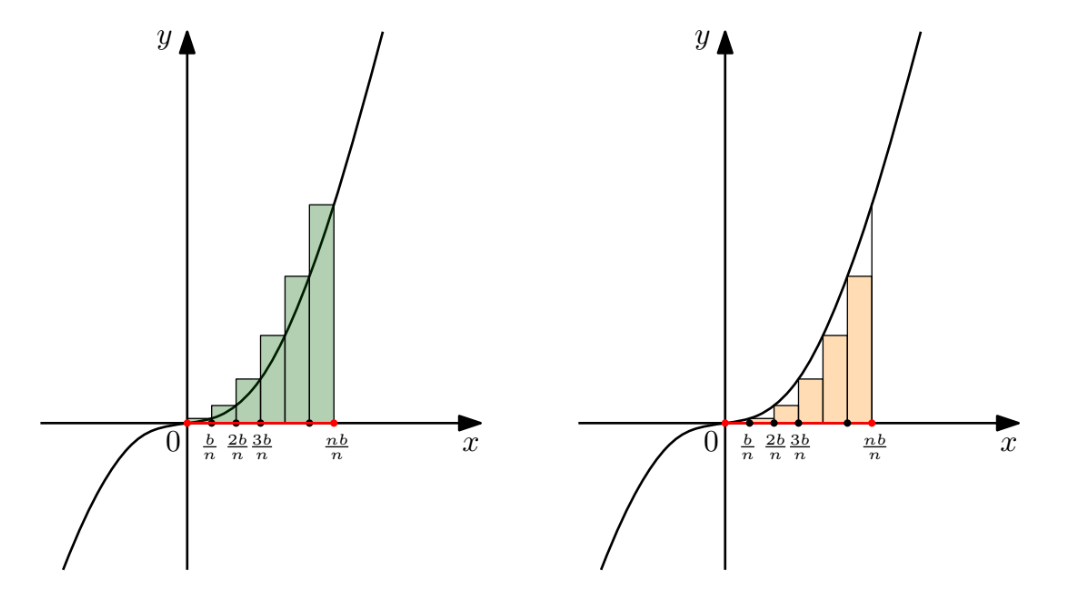
\includegraphics[width=0.7\textwidth]{img/lecture24/definite_integral}
		\end{center}
	\end{example}
	
	\begin{explanation}
	Площадь столбиков на левой картинке:
	\[ S_1 = \sum_{k = 1}^n \bigg(\frac{kb}{n}\bigg)^3 \frac{b}{n} = \sum_{k = 1}^n \frac{b^4}{n^4} \cdot k^3 = \frac{b^4}{n^4} \sum_{k = 1}^n k^3 = \frac{b^4}{n^4} (1 + 2 + ... + n)^2 (*) = \frac{b^4}{n^4} \frac{(n + 1)^2n^2}{4} \]
	
	(*) Формула суммы кубов доказывается по индукции.
	
	Площадь фигуры под графиком заведомо покрывается зелёными столбиками.
	
	Площадь столбиков на правой картинке:
	\[ S_2 = \sum_{k = 1}^n \bigg(\frac{(k - 1)b}{n}\bigg)^3 \frac{b}{n} = \sum_{k = 1}^n \frac{(k - 1)^3b^4}{n^4} \cdot k^3 = \frac{b^4}{n^4} \sum_{k = 1}^n (k - 1)^3 = \frac{b^4}{n^4} (1 + 2 + ... + n)^2 = \]
	\[ = \frac{b^4}{n^4} \frac{(n - 1)^2n^2}{4} \]
	
	Сумма $S_2$ меньше площади фигуры под графиком.
	\[ \lim_{n \to \infty} S_1 = \lim_{n \to \infty} \frac{b^4}{n^4} \frac{(n + 1)^2n^2}{4} = \lim_{n \to \infty} \frac{b^4}{4} \frac{(n + 1)^2}{n^2} = \lim_{n \to \infty} \frac{b^4}{4} \bigg(1 + \frac{1}{n}\bigg)^2 = \frac{b^4}{4} \]
	\[ \lim_{n \to \infty} S_2 = \lim_{n \to \infty} \frac{b^4}{n^4} \frac{(n - 1)^2n^2}{4} = \lim_{n \to \infty} \frac{b^4}{4} \frac{(n - 1)^2}{n^2} = \lim_{n \to \infty} \frac{b^4}{4} \bigg(1 - \frac{1}{n}\bigg)^2 = \frac{b^4}{4} \]
	
	По теореме о зажатой последовательности площадь фигуры равна $\frac{b^4}{4}$. Но можно было получить ответ, посчитав интеграл: $\displaystyle\int x^3 dx = \frac{x^4}{4} + C$.
	\end{explanation}
	
	\section{Интеграл Римана}
	
	\begin{definition}
		\begin{itemize}
			
			\item \underline{Разбиением} $T$ отрезка $[a, b]$ называется набор точек
			$a = x_0 < x_1 < ... < x_n = b$.
			
			\item Отрезки $[x_{k - 1}, x_k]$ называются \underline{отрезками разбиения}. Длину отрезка $[x_{k - 1}, x_k]$ обозначим через $\Delta x_k = x_k - x_{k - 1}, k \geqslant 1$.
			
			\item Величина $\Delta_T := \displaystyle \max_{1 \leqslant k \leqslant n} \Delta x_k$ называется \underline{диаметром разбиения}.
			
			\item \underline{Размеченным разбиением} $(T, \xi)$ отрезка $[a, b]$ называется пара, состоящая из разбиения $T$ отрезка $[a, b]$ и набора точек $\xi = (\xi_1, ..., \xi_n), \xi_k \in [x_{k - 1}, x_k]$.
			
			\item \underline{Интегральной суммой} функции $f$, соответствующей размеченному разбиению $(T, \xi)$, называется выражение
			\[ \sigma(f, T, \xi) := \sum^{n}_{k = 1} f(\xi_k) \Delta x_k. \]
		\end{itemize}
	\end{definition}
	
	\begin{definition}
		Функция $f$ называется интегрируемой по Риману на отрезке
		$[a, b]$, если существует такое число $I$, что $\forall \epsilon > 0$ $\exists \delta > 0: \forall$ размеченного разбиения $(T, \xi)$ с диаметром разбиения $\Delta_T < \delta$ выполнено $|\sigma(f, T, \xi) - I| < \epsilon$.
		
		Число $I$ называют интегралом функции $f$ на отрезке $[a, b]$ и
		обозначают $\displaystyle\int^{b}_{a} f(x) \; dx$.
	\end{definition}
	
	\begin{explanation}
		Геометрически мы уменьшаем длину отрезков и увеличиваем их число.
	\end{explanation}
	
	\begin{example}
		\begin{enumerate}
			\item $\displaystyle\int^{b}_{a} 1 \; dx = b - a$;
			\item Функция $I_{\Q}$ не интегрируема ни на каком отрезке.
		\end{enumerate}	
	\end{example}
	
	\begin{explanation}
		\begin{enumerate}
			\item $\sigma(f, T, \xi) = \sum^{n}_{k = 1} f(\xi_k) \Delta x_k = \sum^{n}_{k = 1} 1 \cdot \Delta x_k = \sum^{n}_{k = 1} \Delta x_k = b - a.$ (функция $f(\xi_k) = 1$ $\forall k$)
			
			\item Функция Дирихле $I_{\Q} : \R \rightarrow {0, 1}$ определяется следующим образом:
			\[\displaystyle I_{\Q} = \left\{{
				\begin{matrix}
					1, & x \in \Q \\
					0, & x \in \I
				\end{matrix}
			}\right.\]
			$\forall$ разбиения $T$ можно взять $\xi \in \Q$, $\zeta \in \I$ (внутри любого отрезка разбиения можно взять рациональное и иррациональное число)
			
			Тогда $\sigma(I_{\Q}, T, \xi) = \sum^{n}_{k = 1} I_{\Q}(\xi_k) \Delta x_k = \sum^{n}_{k = 1} 1 \cdot \Delta x_k = \sum^{n}_{k = 1} \Delta x_k = b - a$ и $\sigma(I_{\Q}, T, \zeta) = \sum^{n}_{k = 1} I_{\Q}(\zeta_k) \Delta x_k = \sum^{n}_{k = 1} 0 \cdot \Delta x_k = 0$.
			
			Тогда для любого $T$ с любым диаметром разбиения можно взять разметку, такую что иногда сумма равна $b - a$, иногда 0. Если $b - a \neq 0$, то функция не интегрируема.
		\end{enumerate}	
	\end{explanation}
    
    \section*{Лекция 25: Интеграл Римана, суммы Дарбу}
    
    \begin{sentence}
    	Если функция $f$ интегрируема по Риману на отрезке $[a, b]$, то она ограничена на этом отрезке.
    \end{sentence}
    
    \begin{proof}
    	Пусть $f$ - интегрируема на $[a, b]$. 
    	
    	Тогда $\exists I \in \R : \forall \epsilon > 0$ $\exists \delta > 0$  $\forall (T, \xi)$ с $\Delta_T < \delta \rightarrow |\sigma(f, T, \xi) - I| < \epsilon \Leftrightarrow$ $\Leftrightarrow I - \epsilon < \sigma(f, T, \xi) < I + \epsilon$.
    	
    	$\sigma(f, T, \xi) = \sum^{n}_{k = 1} f(\xi_k) \Delta x_k.$
    	
    	Пусть $f$ - неограничена на $[a, b] \Rightarrow$ неограничена на одном из отрезков $\Delta_k,$ пусть на $\Delta_{k_0}$. Фиксируем $\xi_k$ для всех $k$ кроме $k_0$. Тогда $\sigma(f, T, \xi) = \sum^{n}_{k = 1} f(\xi_k) \Delta x_k = C + f(\xi_{k_0}) \Delta x_{k_0} \Rightarrow I - C - \epsilon < f(\xi_{k_0}) \Delta x_{k_0} < I - C + \epsilon \Rightarrow \frac{I - C - \epsilon}{\Delta x_{k_0}} < f(\xi_{k_0}) < \frac{I - C + \epsilon}{\Delta x_{k_0}}$ - противоречие, функция ограничена.
    \end{proof}
    
    \begin{sentence}[Линейность интеграла]
    	Пусть $f$ и $g$ интегрируемы по Риману на отрезке $[a, b]$. Тогда
    	для произвольных чисел $\alpha$, $\beta$ функция $\alpha f + \beta g$ интегрируема по Риману на отрезке $[a, b]$ и
    	\[ \displaystyle\int^b_a \alpha f(x) + \beta g(x) \; dx = \alpha \displaystyle\int^b_a f(x) \; dx + \beta \displaystyle\int^b_a g(x) \; dx. \]
    \end{sentence}
    
    \begin{proof}
    	$f$ - интегрируема на $[a, b] \Rightarrow \forall \epsilon > 0$ $\exists \delta_1 > 0 : \forall (T, \xi)$ с $\Delta_T < \delta_1 \rightarrow |\sigma(f, T, \xi) - I_1| < \epsilon.$ 
    	
    	$g$ - интегрируема на $[a, b] \Rightarrow \forall \epsilon > 0$ $\exists \delta_2 > 0 : \forall (T, \xi)$ с $\Delta_T < \delta_2 \rightarrow |\sigma(g, T, \xi) - I_2| < \epsilon.$
    	
    	Размеченное разбиение $(T, \xi)$ взяли одно и то же для обоих интегралов.
    	
    	Первые два утверждения означают, что $I_1 = \int_a^b f(x) \; dx, I_2 = \int_a^b g(x) \; dx.$
    	
    	Рассмотрим интегральную сумму 
    	\[ \sigma(\alpha f + \beta g, T, \xi) = \sum_{k = 1}^n (\alpha f(\xi_k) + \beta g(\xi_k)) \Delta x_k = \sum_{k = 1}^n \alpha f(\xi_k) \Delta x_k + \sum_{k = 1}^n \beta g(\xi_k) \Delta x_k = \]
    	\[ = \alpha \sigma(f, T, \xi) + \beta \sigma(g, T, \xi) \]
    	
    	Фиксируем $\epsilon > 0$ и возьмём $\delta = \min{(\delta_1, \delta_2)} \Rightarrow |\sigma(\alpha f + \beta g, T, \xi) - \alpha I_1 - \beta I_2| = |\alpha \sigma(f, T, \xi) + \beta \sigma(g, T, \xi) - \alpha I_1 - \beta I_2| \leqslant |\alpha \sigma(f, T, \xi) - \alpha I_1| + |\beta \sigma(g, T, \xi) - \beta I_2| \leqslant |\alpha| \epsilon + |\beta| \epsilon = (|\alpha| + |\beta|) \epsilon$
    	
    	$\forall \epsilon = \frac{\epsilon'}{2(|\alpha| + |\beta|)} > 0$ $\exists \delta = \min{(\delta_1, \delta_2)} > 0 : \forall (T, \xi)$ с $\Delta_T < \delta \rightarrow |\sigma(\alpha f + \beta g, T, \xi) - \alpha I_1 - \beta I_2| \leqslant (|\alpha| + |\beta|) \frac{\epsilon'}{2(|\alpha| + |\beta|)} = \frac{\epsilon'}{2} < \epsilon'.$ 
    \end{proof}
    
    \begin{sentence}[Монотонность интеграла]
    	Пусть $f$ и $g$ интегрируемы по Риману на отрезке $[a, b]$. Если
    	$f(x) \leqslant g(x)$ $\forall x \in [a, b],$ то $\displaystyle\int^b_a f(x) \; dx \leqslant \displaystyle\int^b_a g(x) \; dx.$
    \end{sentence}
    
    \begin{proof}
    	$f(x) \leqslant g(x) \Leftrightarrow g(x) - f(x) \geqslant 0$ и $\int_a^b f(x) \; dx \leqslant \int_a^b g(x) \; dx \Leftrightarrow \int_a^b g(x) - f(x) \; dx \geqslant 0$ (пользуемся линейностью). Пусть $h(x) = g(x) - f(x) \Rightarrow$ требуется доказать, что $h(x) \geqslant 0 \Rightarrow \int_a^b h(x) \geqslant 0$.
    	
    	По определению $\forall \epsilon > 0$ $\exists \delta > 0 : \forall (T, \xi)$ c $\Delta_T < \delta \rightarrow  |\sigma(h, T, \xi) - \int_a^b h(x) \; dx| < \epsilon \Leftrightarrow \int_a^b h(x) \; dx - \epsilon < \underline{\sigma(h, T, \xi) < \int_a^b h(x) \; dx + \epsilon}$.
    	
    	$\sigma(h, T, \xi) \geqslant 0 (\text{т. к. } h(\xi_k) \geqslant 0 \Rightarrow \sum_{k = 1}^n h(\xi_k) \Delta x_k \geqslant 0) \Rightarrow \int_a^b h(x) + \epsilon > 0$ $\forall \epsilon > 0 \Rightarrow \int_a^b h(x) > -\epsilon$ $\forall \epsilon > 0 \Rightarrow \int_a^b h(x) \geqslant 0.$
    \end{proof}
    
    \begin{mention}
    	В частности, $\bigg|\displaystyle\int^b_a f(x) \; dx\bigg| \leqslant \displaystyle\int^b_a |f(x)| \; dx.$
    \end{mention}
    
    \begin{proof}
    	Далее мы докажем, что если $f(x)$ интегрируема, то и $|f(x)|$ интегрируема.
    	\[ -|f(x)| \leqslant f(x) \leqslant |f(x)|  \Rightarrow -\int_a^b |f(x)| \; dx \leqslant \int_a^b f(x) \; dx \leqslant \int_a^b |f(x)| \; dx \Rightarrow \]
    	\[ \Rightarrow \bigg| \int_a^b f(x) \; dx \bigg| \leqslant \int_a^b |f(x)| \; dx \]
    \end{proof}
    
    \chapter{Критерий Дарбу и классы интегрируемых функций}
    
    \section{Суммы и интегралы Дарбу}
    
    Фиксируем ограниченную функцию $f$, определённую на отрезке $[a, b]$.
    
    \begin{definition}
    	Для ограниченной на отрезке $[a, b]$ функции $f$ и разбиения $T$ определим \underline{нижнюю и верхнюю суммы Дарбу}:
    	\[s(f, T) := \sum^n_{k = 1}\inf_{x \in [x_{k - 1}, x_k]} f(x) \Delta x_k;\] (на каждом отрезке берём минимальное значение функции)
    	\[S(f, T) := \sum^n_{k = 1}\sup_{x \in [x_{k - 1}, x_k]} f(x) \Delta x_k.\] (на каждом отрезке берём максимальное значение функции)
    	
    	\underline{Нижним интегралом Дарбу} называется число $I_{*} = \displaystyle\sup_{T} s(f, T)$, а \underline{верхним ин-}
    	\underline{тегралом Дарбу} называется число $I^{*} = \displaystyle\inf_{T} S(f, T).$
    \end{definition}
    
    Сумма зелёных прямоугольников - это $s(f, T)$, сумма красных прямоугольников - это $S(f, T)$.
    
    \begin{center}
    	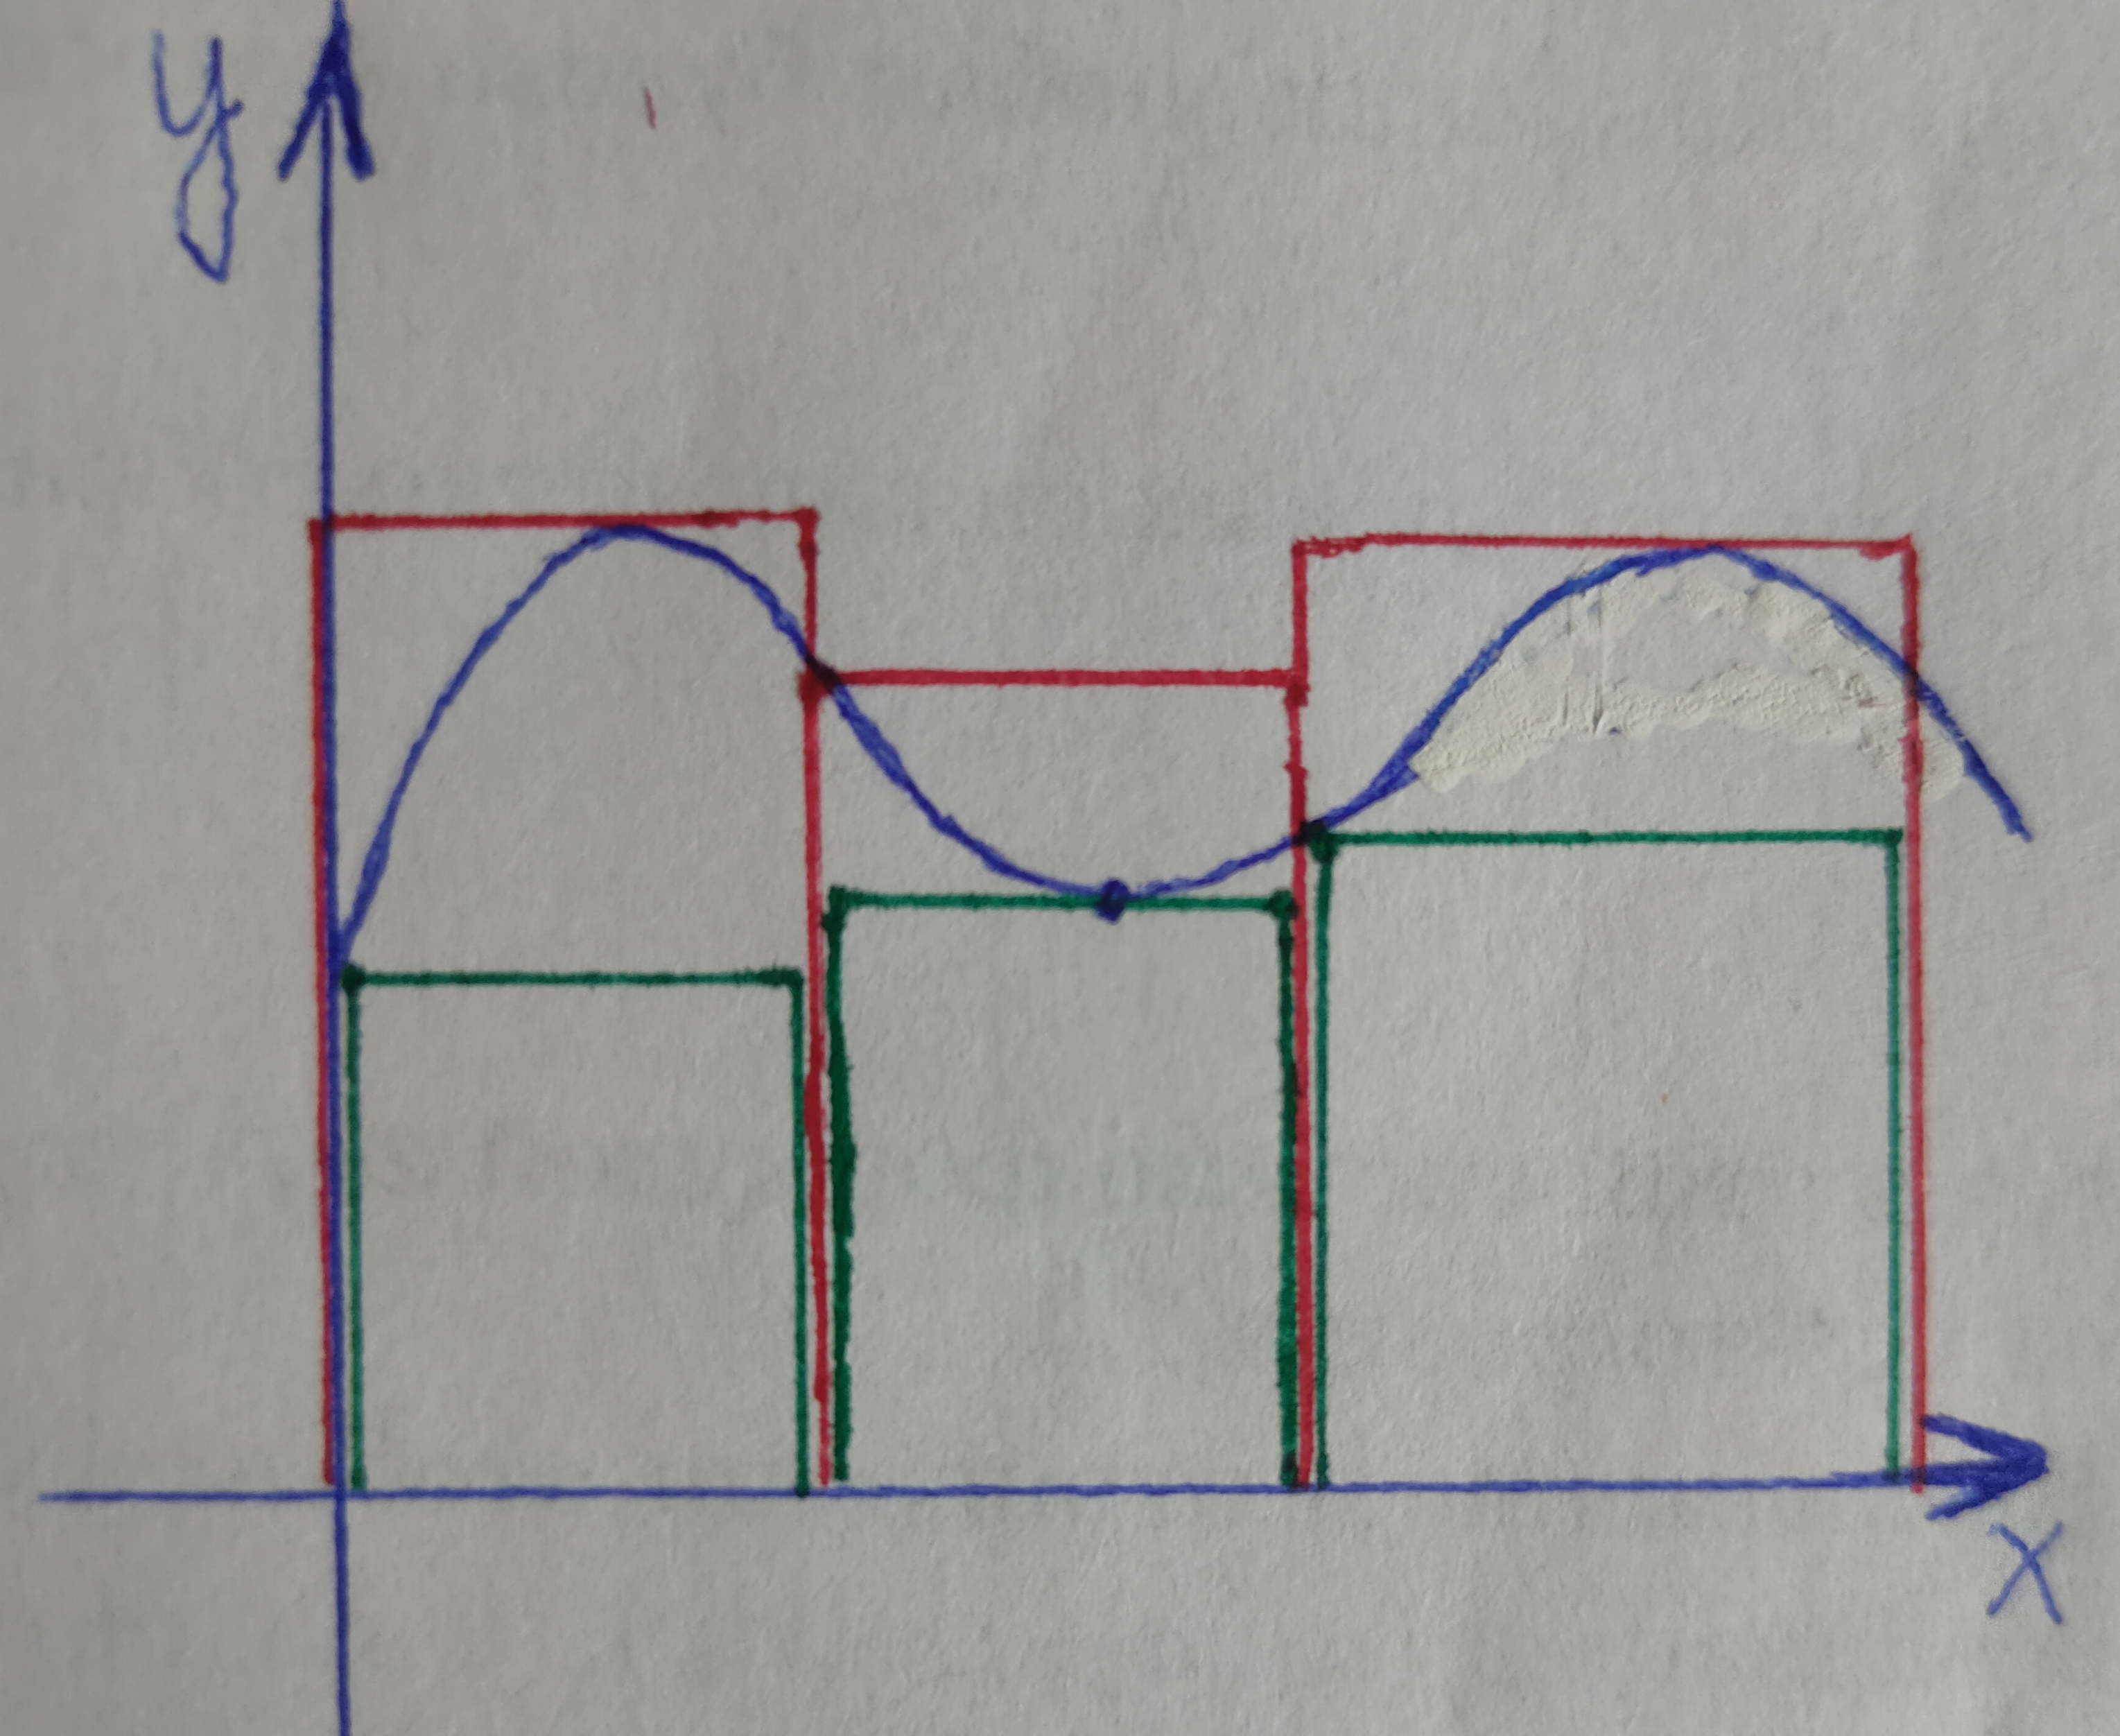
\includegraphics[width=0.4\textwidth]{img/lecture25/integral_darbu}
    \end{center}
    
    \section{Критерий Дарбу}
    
    \begin{lemma}
    	\begin{enumerate}
    		\item $s(f, T) \leqslant \displaystyle\inf_{\xi} \sigma(f, T, \xi) \leqslant \sigma(f, T, \xi) \leqslant \sup_{\xi}{\sigma(f, T, \xi)} \leqslant S(f, T);$
    		\item Если $T \subset T'$, то $s(f, T) \leqslant s(f, T')$ и $S(f, T') \leqslant S(f, T);$
    		\item $s(f, T_1) \leqslant s(f, T_1 \cup T_2) \leqslant S(f, T_1 \cup T_2) \leqslant S(f, T_2).$ 
    	\end{enumerate}
    \end{lemma}
    
    \begin{proof}
    	\begin{enumerate}
    		\item Докажем, что $\displaystyle s(f, T) = \inf_{\xi}{\sigma(f, T, \xi)}$
    		\begin{enumerate}
    			\item[$\leqslant$:] 
    			
    			$\forall \xi$ $\displaystyle s(f, T) = \sum_{k = 1}^n \inf_{\xi_k}{f(\xi_k) \Delta x_k} \leqslant \sum_{k = 1}^n f(\xi_k) \Delta x_k \Rightarrow s(f, T)$ - нижняя грань $\displaystyle \sum_{k = 1}^n f(\xi_k) \Delta x_k$.
    			
    			$\displaystyle \inf_{\xi}{\sum_{k = 1}^n f(\xi_k) \Delta x_k} = \inf_{\xi}{\sigma(f, T, \xi)}$ - точная нижняя грань $\Rightarrow \displaystyle s(f, T) \leqslant \inf_{\xi}{\sigma(f, T, \xi)}$.
    			
    			\item[$\geqslant$:] $\displaystyle s(f, T) = \sum_{k = 1}^n \inf_{\xi_k}{f(\xi_k) \Delta x_k}$
    			
    			По определенению инфимума $\forall \epsilon > 0$ $\displaystyle \exists \xi'_k \in \Delta_k : f(\xi'_k) \leqslant  \inf_{\xi_k}{f(\xi_k)} + \epsilon.$
    			
    			$\displaystyle \sigma(f, T, \xi') = \sum_{k = 1}^n f(\xi'_k) \Delta x_k \leqslant \sum_{k = 1}^n \bigg(\inf_{\xi_k}{f(\xi_k)} + \epsilon \bigg) \Delta x_k = s(f, T) + \epsilon(b - a)$
    			
    			$\displaystyle \inf_{\xi}{\sigma(f, T, \xi)} \leqslant \sigma(f, T, \xi') \leqslant s(f, T) + \epsilon(b - a)$
    			
    			При $\epsilon \to 0$ $\displaystyle \inf_{\xi}{\sigma{(f, T, \xi)}} \leqslant s(f, T)$.
    		\end{enumerate}
    		Второе и третье неравенство в цепочке очевидное.
    		Четвёртое неравенство на самом деле является равенством и доказывается как первое равенство.
    		\item Рассмотрим отрезок $[a, b]$. На нём определено разбиение $T$. Теперь рассмотрим измельчение разбиения $T'$. Оно содержит те же точки, что и в $T$, но добавляет ещё свои точки.
    		
    		Красные точки - точки разбиения $T$, красные и зелёные точки - точки измельчения $T'$.
    		\begin{center}
    			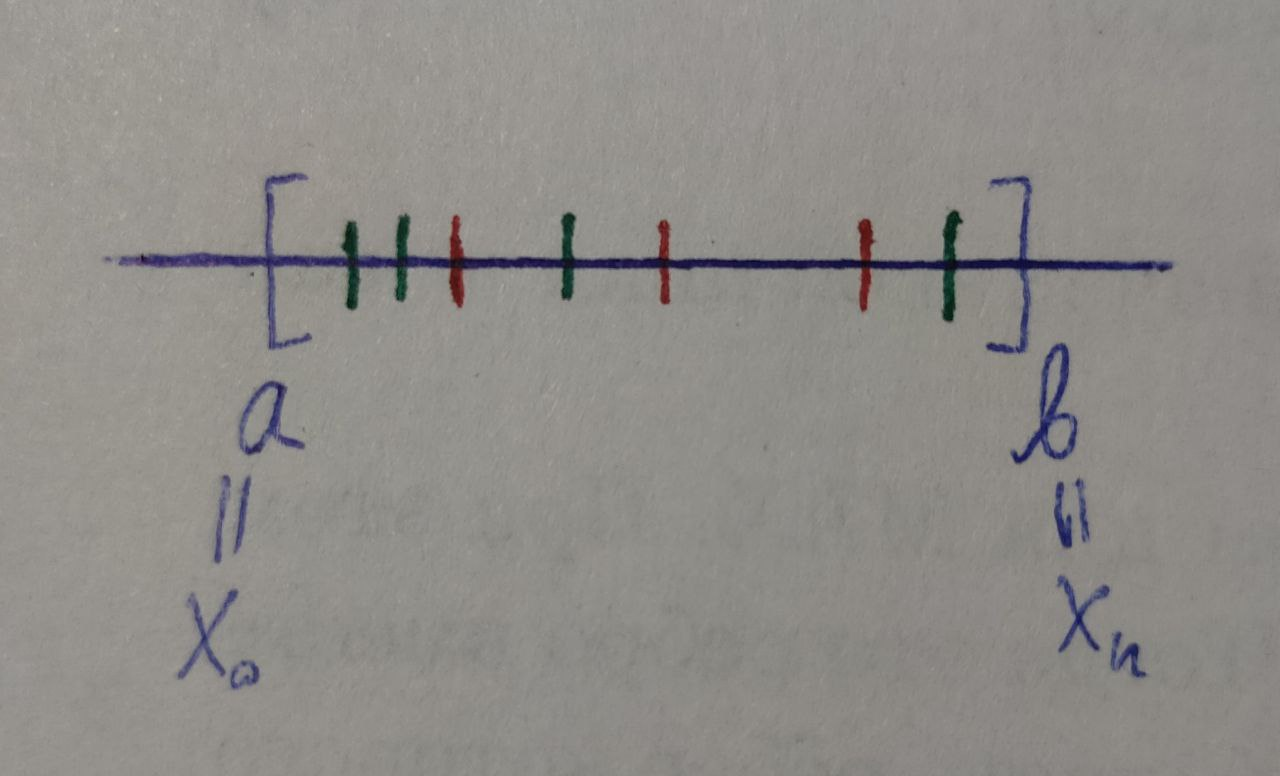
\includegraphics[width=0.3\textwidth]{img/lecture26/segment_division}
    		\end{center}
    		Пусть подотрезки $\Delta_k \in T$, а подотрезки $\Delta'_k \in T'$, $T \subset T'$. Рассмотрим отрезок $\Delta_k$ и будем считать, что он разбился на $k_j$ отрезков. Поэтому отрезок $\Delta'_k$ мы будем индексировать двумя индексами, первый номер - номер отрезка $\Delta_k$, в которым он лежит, второй номер - номер отрезка $\Delta'_k$ внутри отрезка $\Delta_k$.
    		\begin{center}
    			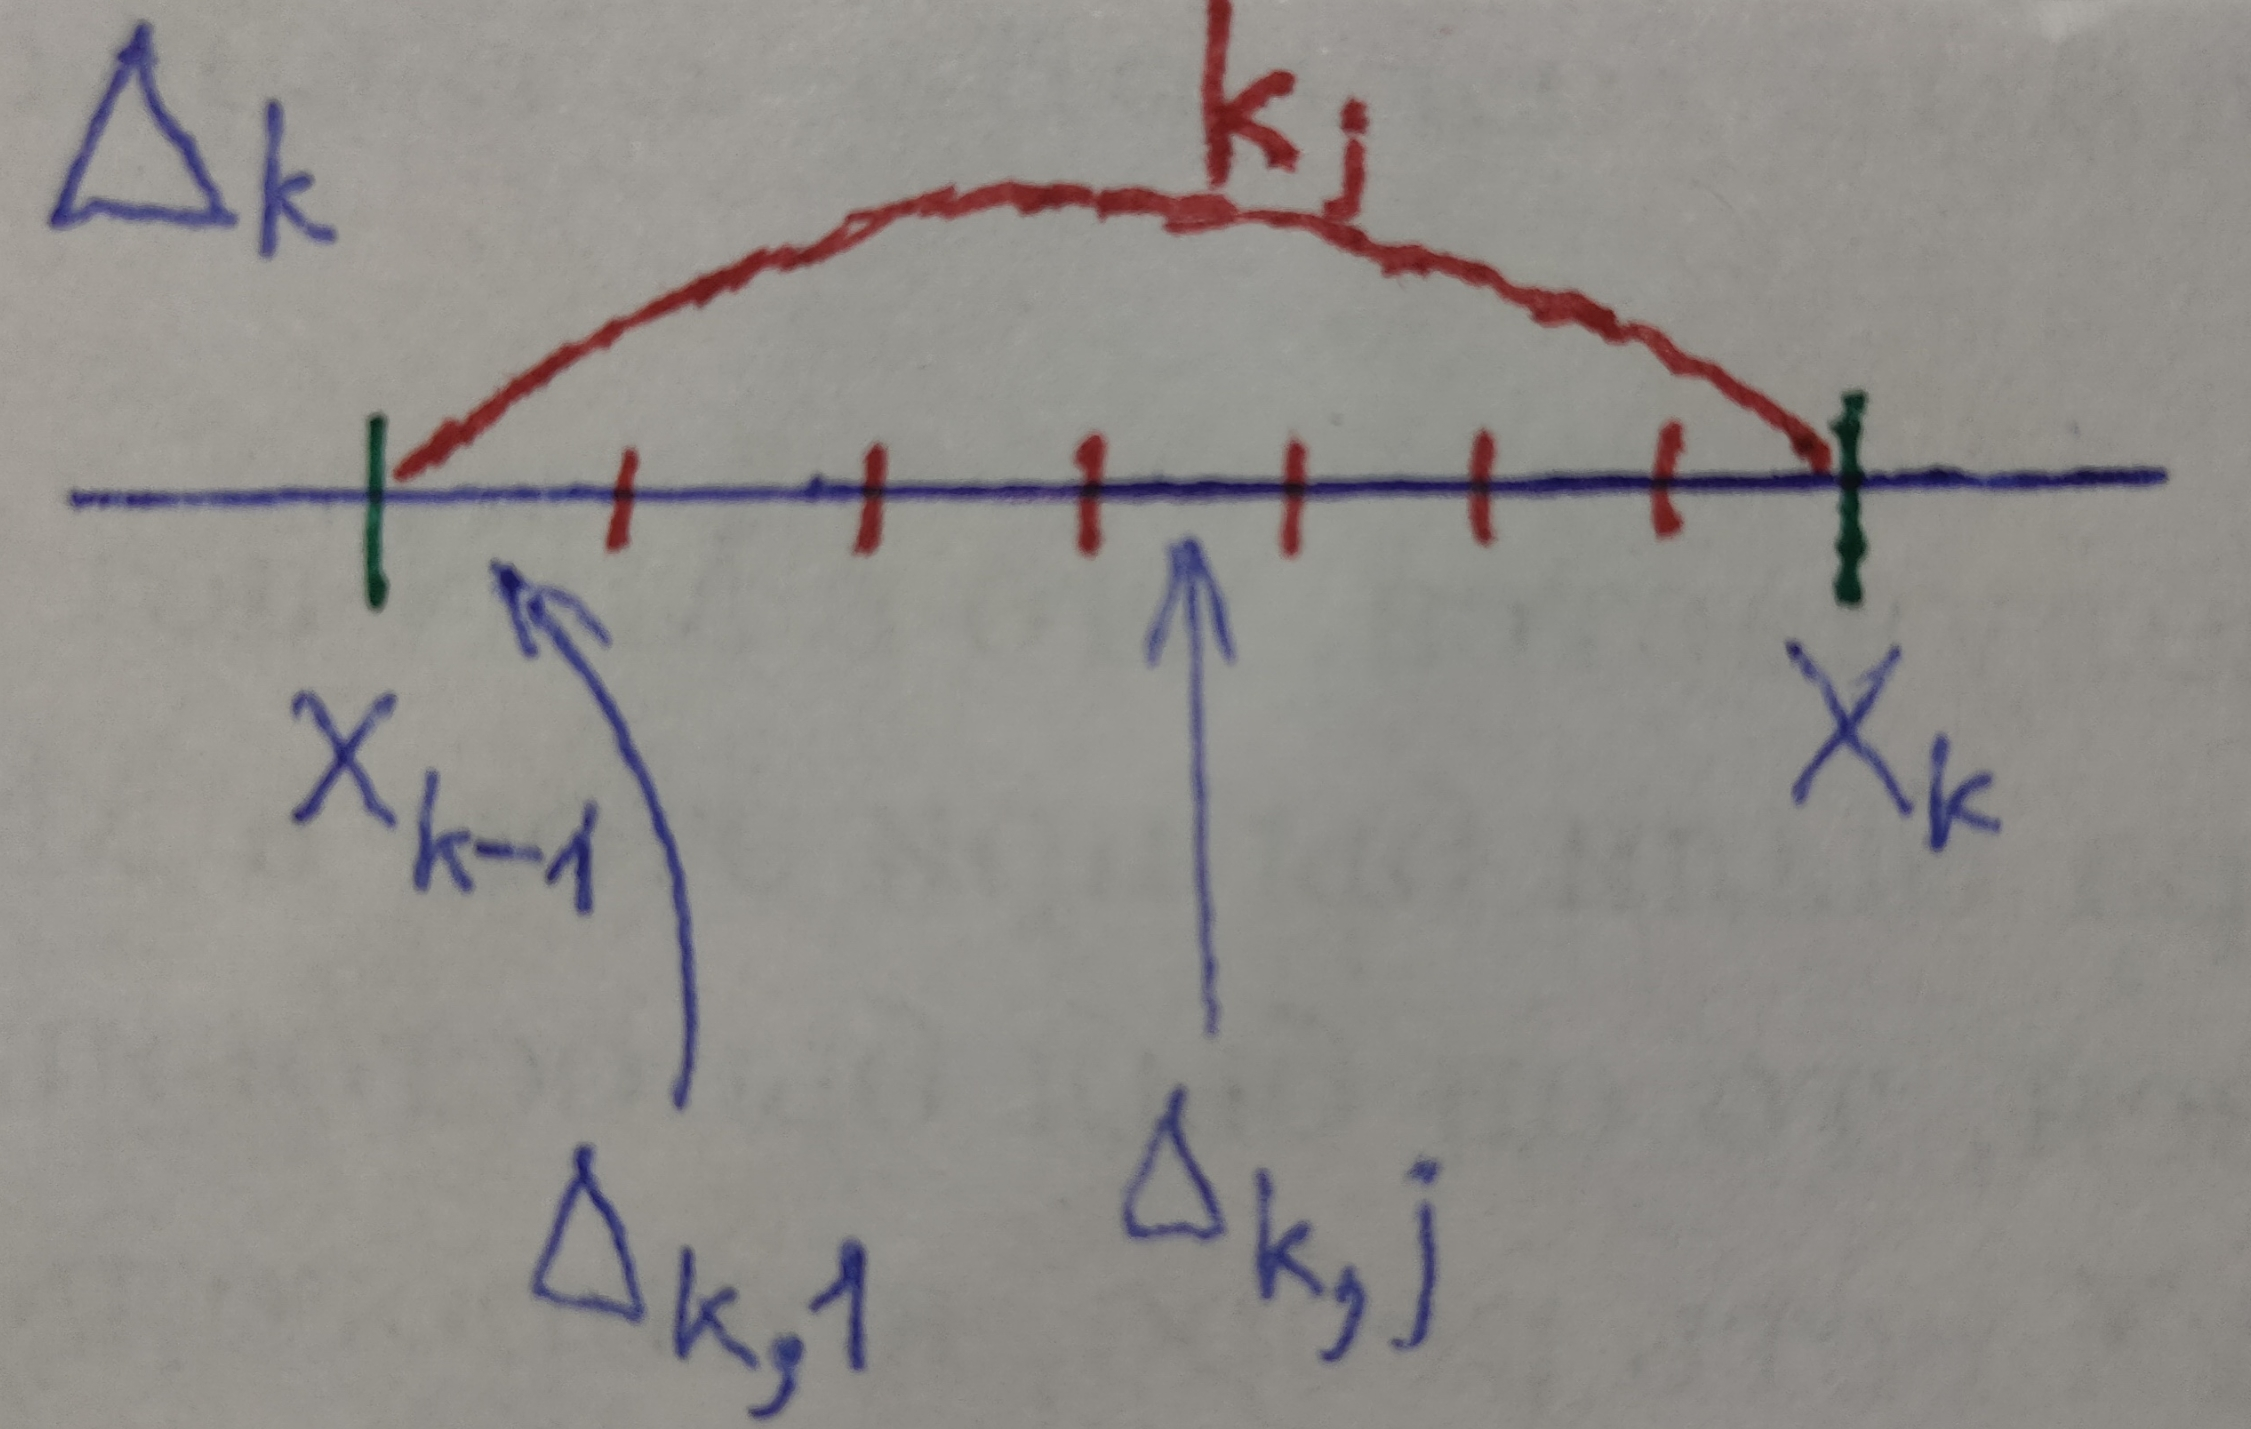
\includegraphics[width=0.3\textwidth]{img/lecture26/notations}
    		\end{center}
    		Тогда
    		\[ s(f, T') = \sum_{k = 1}^n\sum_{j = 1}^{k_j} \inf_{\xi \in \Delta_{k, j}}{f(\xi) \cdot \Delta x_{k, j}} \]
    		Приэтом на нескольких маленьких отрезках инфимум не меньше инфимума на одном большом отрезке, потому что на большом отрезке у нас есть больше точек, из которых мы можем выбрать меньшее значение. Если инфимум достигался на красном отрезке, то этот отрезок принадлежит большому, поэтому мы можем взять точку принадлежащую красному отрезку и получить инфимум на большом отрезке не больше, чем на маленьких. Поэтому
    		\[ s(f, T') = \sum_{k = 1}^n\sum_{j = 1}^{k_j} \inf_{\xi \in \Delta_{k, j}}{f(\xi) \cdot \Delta x_{k, j}} \geqslant \sum_{k = 1}^n\sum_{j = 1}^{k_j} \inf_{\xi \in \Delta_k}{f(\xi) \cdot \Delta x_{k, j}} \]
    		Продолжаем преобразования.
    		\[ \sum_{k = 1}^n \sum_{j = 1}^{k_j} \inf_{\xi \in \Delta_k}{f(\xi) \cdot \Delta x_{k, j}} = \sum_{k = 1}^n \inf_{\xi \in \Delta_k}{f(\xi) \sum_{j = 1}^{k_j} \Delta x_{k, j}} = \sum_{k = 1}^n \inf_{\xi \in \Delta_k}{f(\xi) \Delta x_k} = s(f, T) \]
    		Второе неравенство доказывается аналогично.
    		\item
    		\[ T_1 \subset T_1 \cup T_2 \Rightarrow \text{(из пункта 2) } s(f, T) \leqslant s(f, T_1 \cup T_2) \]
    		\[ \text{(из пункта 1) } s(f, T_1 \cup T_2) \leqslant S(f, T_1 \cup T_2) \]
    		\[ T_1 \cup T_2 \supset T_2 \Rightarrow \text{(из пункта 2) } S(f, T_1 \cup T_2) \leqslant S(f, T_2) \]
    	\end{enumerate}
    \end{proof}
    
    \section*{Лекция 26: Интеграл Римана, суммы Дарбу}
    
    \begin{lemma}
    	$\forall \epsilon > 0$ $\exists \delta > 0:$ $\forall T$ с $\Delta_T < \delta$ выполнено $I_{*} \leqslant s(f, T) + \epsilon$ и $I^{*} \geqslant S(f, T) - \epsilon$.
    \end{lemma}
    
    \begin{proof}
    	По определению супремума
    	\[ I_{*} = \sup_T{s(f, T)} \Rightarrow \forall \epsilon > 0 \text{ } \exists T_{\epsilon} : I_{*} \leqslant s(f, T_{\epsilon}) + \epsilon \]
    	Рассмотрим произвольное разбиение $T$
    	\[ s(f, T_{\epsilon} \cup T) \geqslant \text{(пункт 2 предыдущей леммы)} s(f, T_{\epsilon}) \geqslant I_{*} - \epsilon \]
    	
    	Точки из разбиения $T$ окрасим в красный цвет, точки из $T_{\epsilon}$ - в чёрный цвет.
    	
    	\begin{center}
    		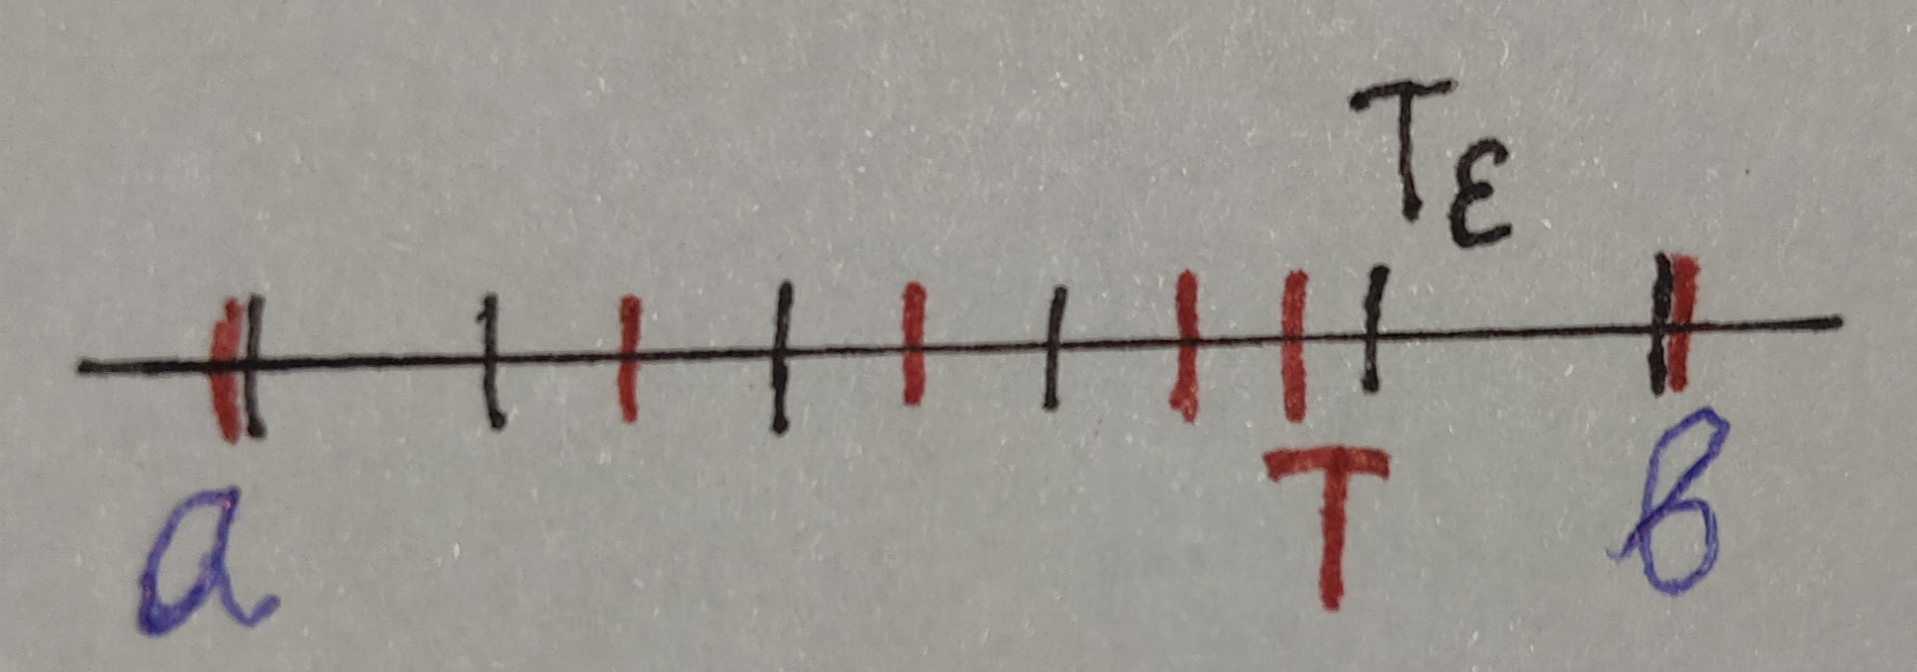
\includegraphics[width=0.2\textwidth]{img/lecture26/coloring_segments}
    	\end{center}
    	
    	Точки $T_{\epsilon}$ делят отрезок c красными концами на число чёрных точек + 1. Тогда точки из $T_{\epsilon}$ могут разбить на не более, чем $2|T_{\epsilon}|$ отрезков, потому что максимум достигается, когда в каждом отрезке мы ставим по одной чёрной точке (т. е. разбиваем отрезок на два).
    	
    	\begin{center}
    		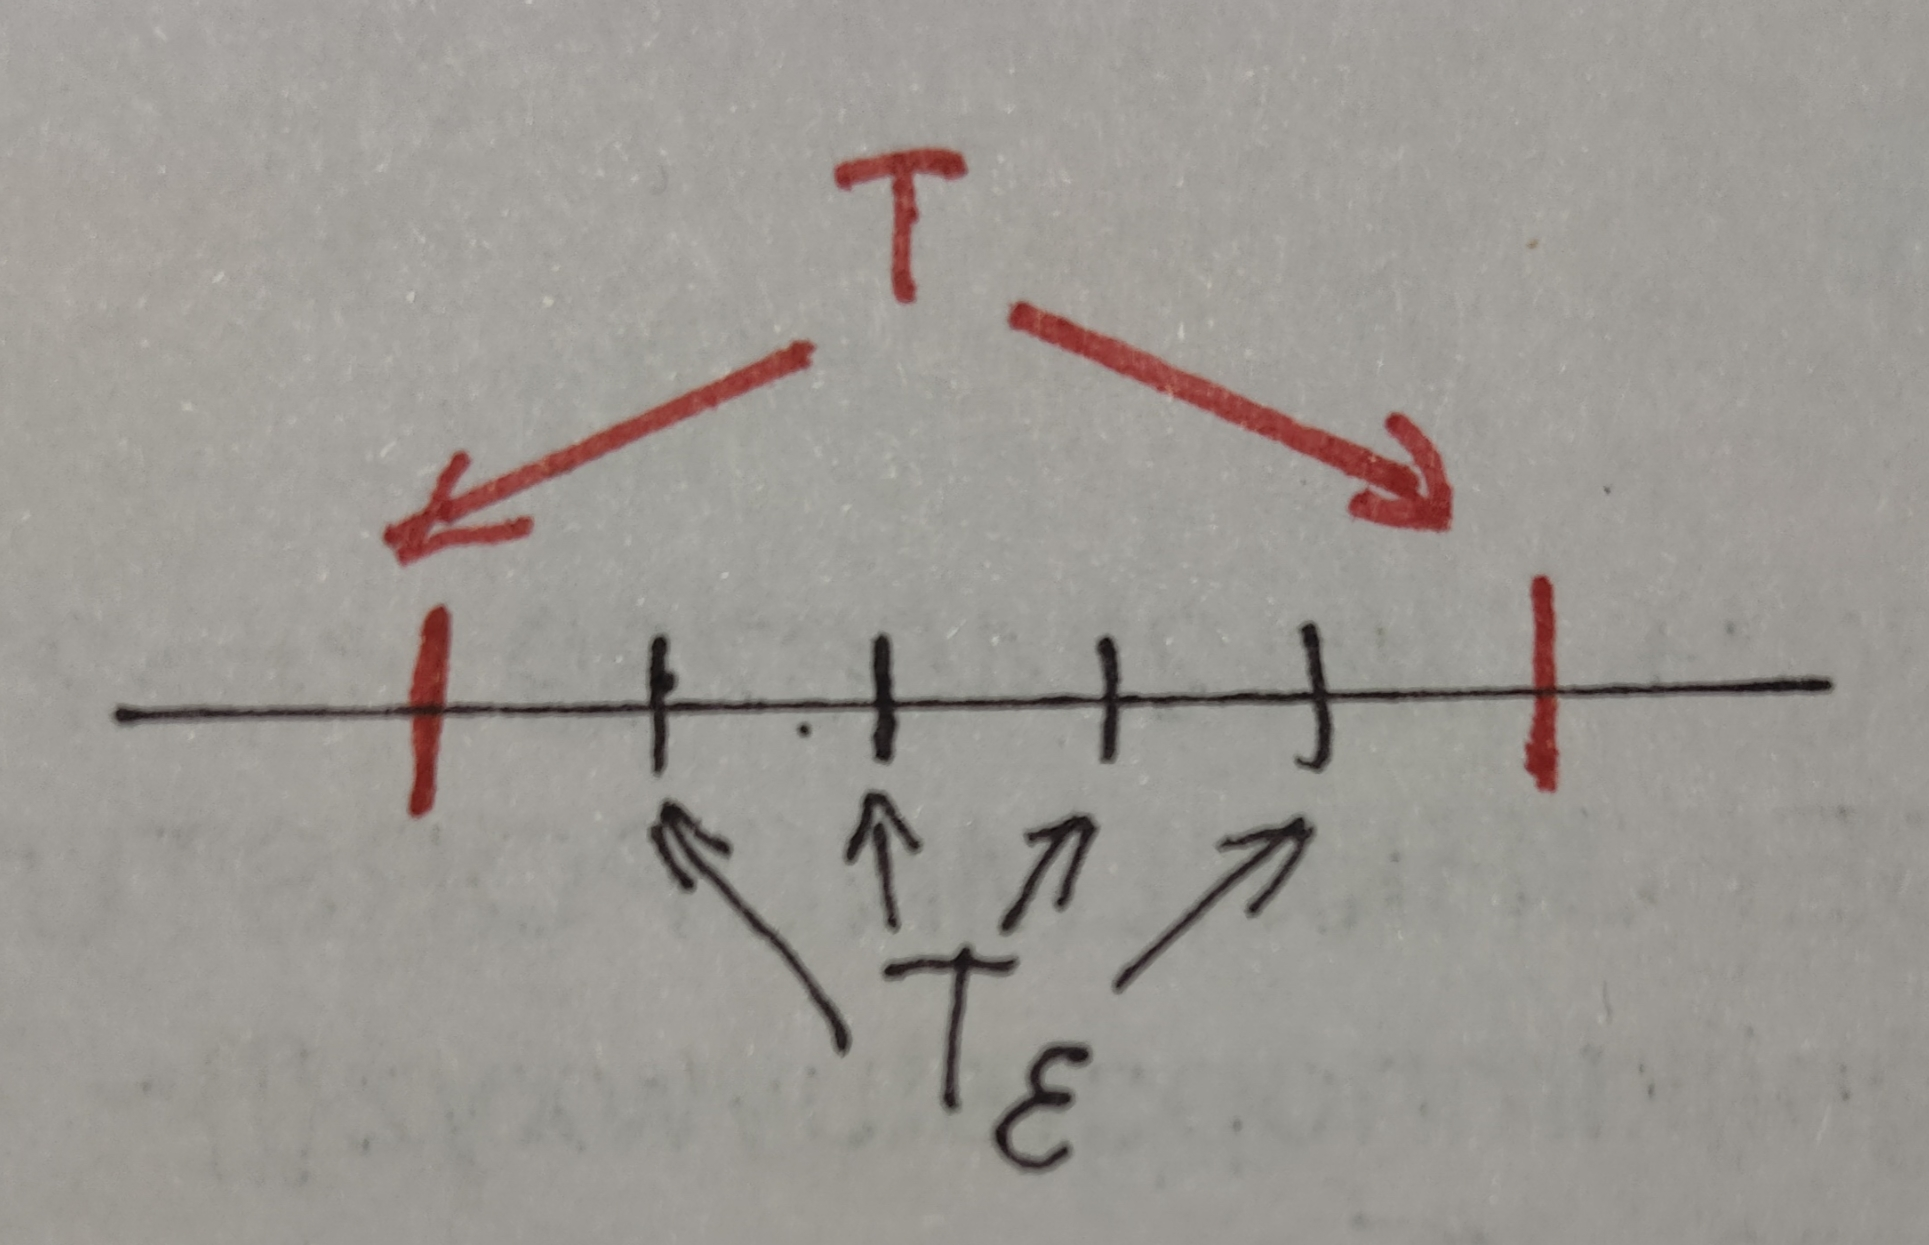
\includegraphics[width=0.2\textwidth]{img/lecture26/segment_number_estimation}
    	\end{center}
    	
    	\underline{Пояснение.} Здесь $\Delta_k$ - отрезок $[x_{k - 1}, x_k]$, подразумеваем под знаком суммы сумму по всем отрезкам, которые образуются этим множеством точек (отрезок образуют соседние точки, т. е. внутри отрезка других точек разбиения нет).
    	\[ s(f, T_{\epsilon} \cup T) = \sum_{\Delta_k \in T_{\epsilon} \cup T} \inf_{\xi \in \Delta_k} {f(\xi) \cdot \Delta x_k} = \sum_{\Delta_k \in T_{\epsilon} \cup T \text{ и } \Delta_k \in T} \inf_{\xi \in \Delta_k} {f(\xi) \cdot \Delta x_k} + \]
    	\[ + \sum_{\Delta_k \in T_{\epsilon} \cup T \text{ и } \Delta_k \not\in T} \inf_{\xi \in \Delta_k} {f(\xi) \cdot \Delta x_k} = (*) \]
    	Первая сумма - сумма отрезков с красными концами, вторая сумма - сумма остальных отрезков (т. е. либо оба конца чёрные, либо один конец чёрный, а другой - красный).
    	Первое слагаемое выразим как разность суммы по всем отрезкам с красными концами и суммы по всем отрезкам с красными концами, но с чёрными точками внутри.
    	\[ (*) = \sum_{\Delta_k \in T} \inf_{\xi \in \Delta_k} {f(\xi) \Delta x_k} - \sum_{\Delta_k \in T \text{ и } \Delta_k \not\in T \cup T_{\epsilon}} {\inf_{\xi \in \Delta_k} {f(\xi) \cdot \Delta x_k}} + \sum_{\Delta_k \in T_{\epsilon} \cup T \text{ и } \Delta_k \not\in T} {\inf_{\xi \in \Delta_k} {f(\xi) \cdot \Delta x_k}} \leqslant \]
    	\[ \leqslant s(f, T) + 2\sup_{x \in [a, b]} {|f(x)| \cdot \Delta_T \cdot 2|T_{\epsilon}|} \]
    	В конце - грубая оценка для последних двух слагаемых.
    	
    	Возьмём $\displaystyle \delta = \frac{\epsilon}{\displaystyle2\sup_{x \in [a, b]} {|f(x)| \cdot 2|T_{\epsilon}|}}$. Тогда для $T$ c $\Delta_T < \delta$
    	\[ I_{*} \leqslant s(f, T_{\epsilon}) + \epsilon \leqslant s(f, T \cup T_{\epsilon}) + \epsilon \leqslant s(f, T) + 2\sup_{x \in [a, b]} {|f(x)| \cdot \Delta_T \cdot 2|T_{\epsilon}|} + \epsilon < \]
    	\[ < s(f, T) + 2\sup_{x \in [a, b]} {|f(x)| \cdot \delta \cdot 2|T_{\epsilon}|} + \epsilon = s(f, T) + \epsilon + \epsilon = s(f, T) + 2\epsilon \]
    	
    	Заменой $\epsilon = \frac{\epsilon'}{2}$ получаем $I_{*} \leqslant s(f, T) + \epsilon'$.
    	
    	Аналогично доказывается, что $I^{*} \geqslant S(f, T) - \epsilon$.
    	
    	\underline{Уточнение.} Если фиксируем $\epsilon$, то $T_{\epsilon}$ - фиксированное число. $f(x)$ интегрируема $\Rightarrow$ она ограничена (по предложению 9.5) $\Rightarrow$ супремум ограничен, поэтому такое $\delta$ рассматривать корректно.
    \end{proof}
    
    \begin{theorem}[Критерий Дарбу]
    	Ограниченная функция $f$ интегрируема по Риману на отрезке $[a, b]$ тогда и только тогда, когда $I^{*} = I_{*}$.
    \end{theorem}
    
    \begin{proof}
    	\begin{enumerate}
    		\item[$\Rightarrow$] Если функция интегрируема, то 
    		\[ \forall \epsilon > 0 \text{ } \exists \delta > 0: \forall (T, \xi) \text{ с } \Delta_T < \delta \rightarrow |\sigma(f, T, \xi) - I| < \epsilon \]
    		\[ I - \epsilon < \sigma(f, T, \xi) < I + \epsilon \]
    		\[ I - \epsilon \leqslant \inf_{\xi} {\sigma(f, T, \xi)} = s(f, T) \leqslant \sup_{T} {s(f, T)} = I_{*} \]
    		\[ I^{*} = \inf_{T} {S(f, T)} \leqslant S(f, T) = \sup_{\xi} {\sigma(f, T, \xi)} \leqslant I + \epsilon \]
    		
    		Докажем, что $I_{*} \leqslant I^{*}$:
    		\[ \forall T_1, T_2 \text{ } s(f, T_1) \leqslant S(f, T_2) \Rightarrow \sup_{T_1} {s(f, T_1)} \leqslant S(f, T_2) \Rightarrow \sup_{T_1} {s(f, T_1)} \leqslant \inf_{T_2} {S(f, T_2)} \]
    		Тогда
    		\[ I - \epsilon \leqslant I_{*} \leqslant I^{*} \leqslant I + \epsilon \]
    		Устремляя $\epsilon \to 0$, получаем, что $I_{*} = I^{*}$.
    		\item[$\Leftarrow$] $I = I_{*} = I^{*}$
    		\[ \forall \epsilon > 0 \text{ } \exists \delta > 0 : \forall T \text{ с } \Delta_T < \delta \rightarrow I - \epsilon = I_{*} - \epsilon \leqslant (\text{лемма 10.3}) \text{ } s(f, T) \leqslant \]
    		\[ \leqslant \sigma(f, T, \xi) \leqslant S(f, T) \leqslant (\text{лемма 10.3}) \text{ } I^{*} + \epsilon = I + \epsilon \Rightarrow |\sigma(f, T, \xi) - I| < \epsilon, \]
    		что есть определение интеграла.
    	\end{enumerate}
    \end{proof}
    
    \section{Колебание функции}
    
    \begin{definition}
    	\underline{Колебанием} функции $f$ на отрезке $\Delta$ называется число
    	\[ \omega(f, \Delta) := \sup_{x, y \in \Delta}{|f(x) - f(y)|} = \sup_{x \in \Delta}{f(x)} - \inf_{y \in \Delta}{f(y)}. \]
    \end{definition}
    
    \begin{explanation}
    	\begin{enumerate}
    		\item В одну сторону
    		\[ \forall x, y \in \Delta \text{ } f(x) - f(y) \leqslant \sup_{x \in \Delta} {(f(x))} - f(y) \leqslant \sup_{x \in \Delta} {f(x)} - \inf_{y \in \Delta} {f(y)} \Rightarrow \]
    		\[ \Rightarrow \sup_{x, y \in \Delta}{|f(x) - f(y)|} \leqslant \sup_{x \in \Delta}{f(x)} - \inf_{y \in \Delta}{f(y)} \] 
    		\item В другому сторону
    		
    		По определению супремума и инфимума
    		\[ \forall \delta > 0 \text{ } \exists x_{\delta}: \sup_{x \in \Delta} {f(x)} \leqslant f(x_{\delta}) + \delta \]
    		\[ \forall \delta > 0 \text{ } \exists y_{\delta}: \inf_{y \in \Delta} {f(y)} \geqslant f(y_{\delta}) - \delta \]
    		Тогда
    		\[ \sup_{x \in \Delta} {f(x)} - \inf_{y \in \Delta}{f(y)} \leqslant f(x_{\delta}) - f(y_{\delta}) + 2\delta \leqslant  \sup_{x, y \in \Delta} {|f(x) - f(y)|} + 2\delta \Rightarrow \]
    		\[ \Rightarrow \sup_{x \in \Delta} {f(x)} - \inf_{y \in \Delta}{f(y)} \leqslant  \sup_{x, y \in \Delta} {|f(x) - f(y)|} \text{ при } \delta \to 0 \]
    	\end{enumerate}
    \end{explanation}
    
    \section*{Лекция 27: Интегрируемость по Риману различных классов функций}
    
    \begin{theorem}
    	Пусть $f$ - ограниченная на отрезке $[a, b]$ функция. Тогда следующие условия эквивалентны:
    	\begin{enumerate}
    		\item $I^{*} = I_{*}$;
    		\item Функция $f$ интегрируема на $[a, b]$;
    		\item $\forall \epsilon > 0$ $\exists \delta > 0: \forall T$ с $\Delta_T < \delta:$
    		\[ \sum_{k = 1}^{n} \omega(f, \Delta_k) \Delta x_k < \epsilon; \]
    		\item $\forall \epsilon > 0$ $\exists T:$
    		\[ \sum_{k = 1}^{n} \omega(f, \Delta_k) \Delta x_k < \epsilon; \]
    	\end{enumerate}
    \end{theorem}
    
    \begin{proof}
    	Заметим, что
    	\[ S(f, T) - s(f, T) = \sum_{k = 1}^n \sup_{\xi \in \Delta_k} f(\xi) \Delta x_k - \sum_{k = 1}^n \inf_{\xi \in \Delta_k} f(\xi) \Delta x_k = \]
    	\[ = \sum_{k = 1}^n \bigg(\sup_{\xi \in \Delta_k} f(\xi) \Delta x_k - \inf_{\xi \in \Delta_k} f(\xi) \Delta x_k\bigg) = \sum_{k = 1}^n \omega(f, \Delta_k) \Delta x_k \]
    	
    	\begin{enumerate}
    		\item[$1 \Rightarrow 2$] Применяем критерий Дарбу.
    		\item[$2 \Rightarrow 3$] Пусть $f$ - интегрируемая функция на $[a, b]$. Тогда $I^{*} = I_{*} = I$.
    		
    		По лемме 10.3
    		\[ \forall \epsilon > 0 \text{ } \exists \delta > 0: \forall T \text{ c } \Delta_T < \delta:
    		\displaystyle \left\{{
    			\begin{matrix}
    				I = I^{*} \geqslant S(f, T) - \epsilon, \\
    				I = I_{*} \leqslant s(f, T) + \epsilon. \\
    			\end{matrix}
    		}\right. \Rightarrow \]
    		\[ \Rightarrow I - I \leqslant s(f, T) - S(f, T) + 2\epsilon \]
    		По замечанию заключаем
    		\[ \sum_{k = 1}^n \omega(f, \Delta_k) \Delta x_k \leqslant 2\epsilon \]
    		\item[$3 \Rightarrow 4$] По предыдущему пункту существует такое $T$ с диаметром $\Delta_T < \delta$, значит и просто $T$ существует.
    		\item[$4 \Rightarrow 1$] В доказательстве критерия Дарбу мы получили следующую цепочку неравенств
    	    \[ s(f, T) \leqslant I_{*} \leqslant I^{*} \leqslant S(f, T) \]
    	    Тогда
    	    \[ 0 \leqslant I^{*} - I_{*} \leqslant S(f, T) - s(f, T) = \sum_{k = 1}^n \omega(f, \Delta_k) \Delta x_k < \epsilon \Rightarrow \text{ при } \epsilon \to 0 \text{ } I^{*} = I_{*} \]
    	\end{enumerate}
    \end{proof}
    
     \section{Интегрируемость модуля, квадрата и произведения функций}
    
    \begin{corollary}
    	Если $f$ интегрируема по Риману на отрезке $[a, b]$, то $|f|$ и $f^2$ интегрируемы по Риману на отрезке $[a, b]$ и для любого $[c, d] \subset [a, b]$ функция $f$ интегрируема по Риману на отрезке
    	$[c, d]$.
    \end{corollary}
    
    \begin{proof}
    	$f$ - интегрируема на $[a, b] \Leftrightarrow$ по пункту 4 теоремы 10.6 
    	\[ \forall \epsilon > 0 \text{ } \exists T: \sum_{k = 1}^n \omega(f, \Delta_k) \Delta x_k < \epsilon. \]
    	\underline{Доказательство для модуля функции}
    	
    	(Неравенство треугольника: $|A| - |B| \leqslant |A - B|, |B| - |A| \leqslant |A - B| \Rightarrow ||A| - |B|| \leqslant |A - B|$)
    	\[ \omega(|f|, \Delta_k) = \sup_{x, y \in \Delta_k} {||f(x)| - |f(y)||} \leqslant \sup_{x, y \in \Delta_k} {|f(x) - f(y)|} = \omega(f, \Delta_k) \Rightarrow \]
    	\[ \Rightarrow 0 \leqslant \sum_{k = 1}^n {\omega(|f|, \Delta_k)} \Delta x_k \leqslant \sum_{k = 1}^n \omega(f, \Delta_k) \Delta x_k < \epsilon \]
    	\underline{Доказательство для квадрата функции}
    	\[ \omega(f^2, \Delta_k) = \sup_{x, y \in \Delta_k} {|f^2(x) - f^2(y)|} = \sup_{x, y \in \Delta_k} {|(f(x) - f(y))(f(x) + f(y))|} \leqslant \]
    	\[ \leqslant \sup_{x, y \in \Delta_k} {|f(x) - f(y)|(|f(x)| + |f(y)|)} \leqslant 2\sup_{x \in \Delta_k} {|f(x)|} \sup_{x, y \in \Delta_k} {|f(x) - f(y)|} = \]
    	\[ = 2\sup_{x \in \Delta_k} {|f(x)|} \cdot \omega(f, \Delta_k) \]
    	\[ \sum_{k = 1}^n \omega(f^2, \Delta_k) \Delta x_k \leqslant \sum_{k = 1}^n 2\sup_{x \in \Delta_k} {|f(x)| \omega(f, \Delta_k) \Delta x_k} \leqslant 2\sup_{x \in [a, b]} |f(x)| \sum_{k = 1}^n \omega(f, \Delta_k) \Delta x_k \leqslant \]
    	\[ \leqslant M \cdot \epsilon, \text{где M - константа}. \]
    	
    	В обоих случаях в конце мы применяем теорему 10.6 и заключаем, что функции интегрируемы на $[a, b]$.
    	
    	Интегрируемость функции на подотрезке докажем далее.
    \end{proof}
    
    \begin{corollary}
    	Если $f$ и $g$ интегрируемы на $[a, b]$, то и $f \cdot g$ интегрируема на $[a, b]$.
    \end{corollary}
    
    \begin{proof}
    	Если $f$ и $g$ интегрируемы, то $f - g$ и $f + g$ интегрируемы. Тогда их квадраты $(f - g)^2$ и $(f + g)^2$ интегрируемы. Следовательно, $\frac{1}{4}((f + g)^2 - (f - g)^2) = \frac{1}{4} \cdot 4fg = fg$ интегрируема.
    \end{proof}
    
    \section{Интегрируемость монотонной функции}
    
    \begin{corollary}
    	Если $f$ монотонна на $[a, b]$, то $f$ интегрируема по Риману на $[a, b]$.
    \end{corollary}
    
    \begin{proof}
    	Без ограничения общности пусть $f$ - возрастающая функция.
    	\[ \omega(f, \Delta_k) = f(x_k) - f(x_{k - 1}) \]
    	\[ \sum_{k = 1}^n \omega(f, \Delta_k) \cdot \Delta x_k = \sum_{k = 1}^n (f(x_k) - f(x_{k - 1})) \Delta x_k = (*) \]
    	Пусть $\Delta x_k = \Delta x_j$ $\forall k, j$. Тогда
    	\[ (*) = \Delta x_1 \sum_{k = 1}^n (f(x_k) - f(x_{k - 1})) = \Delta_T (f(b) - f(a)) \]
    	Следовательно, $\forall T -$ разбиение $[a, b]$ на одинаковые части с $\Delta_T < \frac{\epsilon}{f(b) - f(a)}$
    	\[ \sum_{k = 1}^n \omega(f, \Delta_k) \Delta x_k \leqslant \epsilon. \]
    	
        Для убывающей $f$ доказывается аналогично.
    \end{proof}
    
    \section{Равномерная непрерывность}
    
    \begin{definition}
    	\item Функция $f$ называется \underline{равномерно непрерывной} на
    	множестве $X$, если $\forall \epsilon > 0$ $\exists \delta > 0$ для которого из неравенства
    	$|x - y| < \delta$ следует $|f(x) - f(y)| < \epsilon.$
    \end{definition}
    
    \begin{center}
    	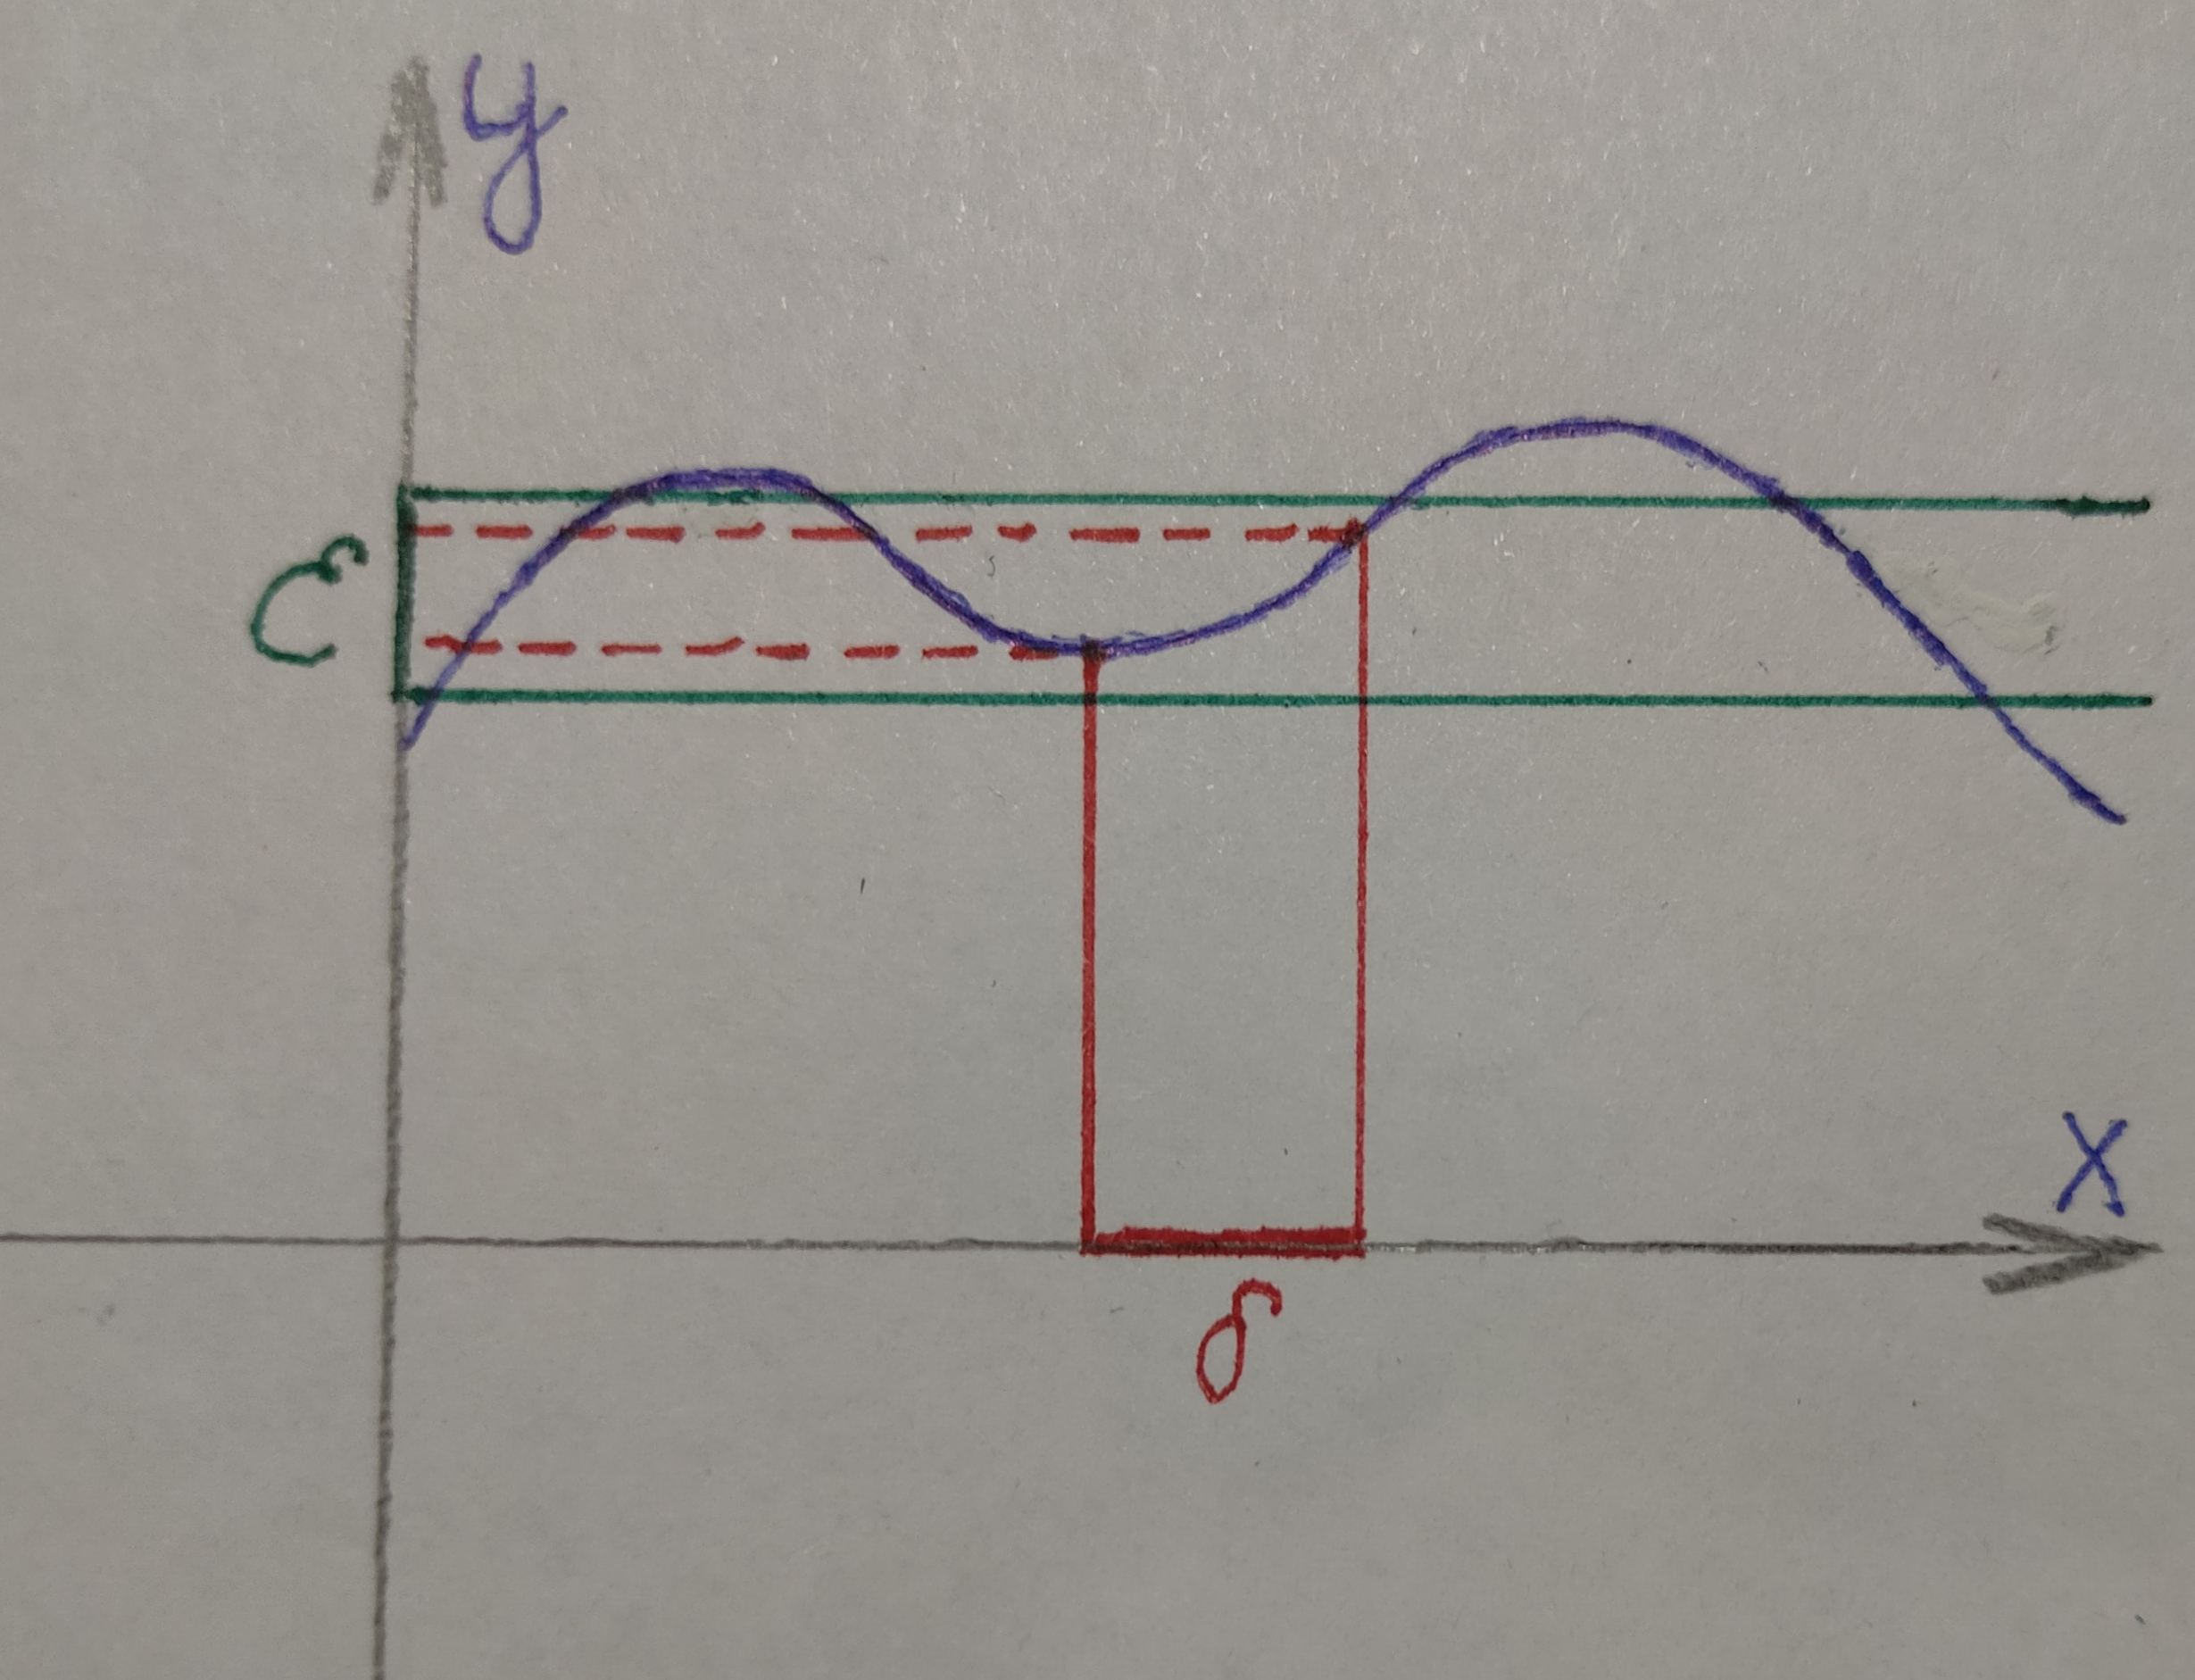
\includegraphics[width=0.5\textwidth]{img/lecture27/uniformly_continuous_function}
    \end{center}
    
    \begin{explanation}
    	Другими словами, существует $\delta$ на оси OX такая, что расстояние между $x$ и $y$ меньше, чем $\delta$, и разность между значениями функции в точках $x$ и $y$ помещается в этот $\epsilon-$корридор.
    \end{explanation}
    
    \begin{mention}
    	Если функция является равномерно-непрерывной, то она является и непрерывной, т. к. определение непрерывности слабее:
    	\[ f - \text{непрерывна на } X \Rightarrow \forall x_0 \in X \text{ } \forall \epsilon > 0 \text{ } \exists \delta > 0: \forall x \in B_{\delta}(x_0) \rightarrow |f(x) - f(x_0)| < \epsilon \]
    	
    	В обратную сторону это не правда, см. пункт 2) примера 10.12.
    \end{mention}
    
    \begin{example}
    	\begin{enumerate}
    		\item Функция $f(x) := \sin{x}$ равномерно непрерывна на $\R$, т.к.
    		по теореме Лагранжа $|\sin{x} - \sin{y}| = |\cos{\xi}| \cdot |x - y| \leqslant |x - y|$.
    		\item Функция $f(x) = \frac{1}{x}$ не равномерно непрерывна на $(0, 1)$,
    		т.к. $f(\frac{1}{2n}) - f(\frac{1}{n}) = n, а |\frac{1}{n} - \frac{1}{2n}| = \frac{1}{2n} \rightarrow 0$.
    	\end{enumerate}
    \end{example}
    
    \begin{explanation}
    	\begin{enumerate}
    		\item По теореме Лагранжа $\forall x, y \in \R |\sin{x} - \sin{y}| = |(\sin{\xi})'(x - y)| = |\cos{\xi}||(x - y)| \leqslant |x - y|$
    		\item Требуется доказать отрицание определения равномерной непрерывности:
    		\[ \exists \epsilon = 1 \text{ } \forall \delta > 0 \text{ } \exists x, y \in (0, 1) \text{ } |x - y| < \delta: |f(x) - f(y)| \geqslant 1 \]
    		Будем доказывать для $\delta = \frac{1}{n}$, потому что всегда можно взять $\frac{1}{n} < \delta$. Тогда пусть $x = x_n = \frac{1}{n}, y = y_n = \frac{1}{2n} \Rightarrow |x - y| = |\frac{1}{n} - \frac{1}{2n}| = \frac{1}{2n} < \frac{1}{n}, |f(x) - f(y)| = |n - 2n| = n \geqslant 1$.
    	\end{enumerate}
    \end{explanation}
    
    \section{Интегрируемость непрерывной функции}
    
    \begin{theorem}[Кантора]
    	Если функция $f$ непрерывна на отрезке $[a, b]$, то $f$ равномерно непрерывна на $[a, b]$.
    \end{theorem}
    
    \begin{proof}
    	Пусть $f$ - непрерывная функция на $[a, b]$, но не равномерно-непрерывная:
    	\[ \exists \epsilon > 0: \forall \delta = \frac{1}{n} > 0 \text{ } \exists x_n, y_n \in [a, b]: |x_n - y_n| < \frac{1}{n} \rightarrow |f(x_n) - f(y_n)| \geqslant \epsilon \]
    	$x_n$ - ограниченная последовательность, т. к. $x_n \in [a, b] \Rightarrow$ по теореме Больцано $\exists x_{n_k} \to x \Rightarrow$ из неравенства $|x_n - y_n| < \frac{1}{n}$ следует, что $x_{n_k} - \frac{1}{n} < y_{n_k} < x_{n_k} + \frac{1}{n}$.
    	$x_{n_k} - \frac{1}{n} \to x, x_{n_k} + \frac{1}{n} \to x \Rightarrow$ по теореме о зажатой последовательности $y_{n_k} \to x$.
    	\[ \epsilon \leqslant |f(x_{n_k}) - f(y_{n_k})| = |f(x_{n_k}) - f(x) + f(x) - f(y_{n_k})| \leqslant |f(x_{n_k}) - f(x)| + |f(x) - f(y_{n_k})| \]
    	Но $|f(x_{n_k}) - f(x)| \to 0, |f(x) - f(y_{n_k})| \to 0$, а $\epsilon > 0$ - противоречие.
    \end{proof}
    
    \begin{corollary}
    	Пусть $f$ непрерывна на $[a, b]$. Тогда $f$ интегрируема по Риману на $[a, b]$.
    \end{corollary}
    
    \begin{proof}
    	В силу предыдущей теоремы $f$ равномерно непрерывна на $[a, b]$. Поэтому 
    	\[ \forall \epsilon > 0 \text{ } \exists \delta > 0 : \forall T \text{ с } \Delta_T < \delta \text{ } \forall x, y \in \Delta_k \rightarrow \sup_{x, y \in \Delta_k} {|f(x) - f(y)|} < \epsilon \text{ } \forall k \Rightarrow \]
    	\[ \Rightarrow \omega(f, \Delta_k) < \epsilon \text{ } \forall k.\]
    	Для такого разбиения $\displaystyle \sum_{k = 1}^n \omega(f, \Delta_k) \Delta x_k < \epsilon |b - a| \Rightarrow$ по теореме 10.6 функция $f$ интегрируема по Риману на $[a, b]$.
    \end{proof}
    
    \section*{Лекция 28: Формула Ньютона-Лейбница}
    
    \section{Аддитивность интеграла}
    
    \begin{corollary}
    	Если $f$ интегрируема по Риману на отрезке $[a, b]$, $[c, d] \subseteq [a, b]$, то $f$ интегрируема на отрезке $[c, d]$.
    \end{corollary}
    
    \begin{proof}
    	$f$ - интегрируема на $[a, b] \Rightarrow$ по теореме 10.6 $\forall \epsilon > 0 \text{ } \exists T:$
    	\[ \sum_{k = 1}^n \omega(f, \Delta_k) \cdot \Delta x_k < \epsilon \Leftrightarrow 0 \leqslant \sum_{k = 1}^n \sup_{x \in \Delta_k} {f(x)} \cdot \Delta_k - \sum_{k = 1}^n \inf_{x \in \Delta_k} {f(x)} \cdot \Delta_k < \epsilon \Leftrightarrow \]
    	\[ \Leftrightarrow 0 \leqslant S(f, T) - s(f, T) < \epsilon \]
    	\begin{center}
    		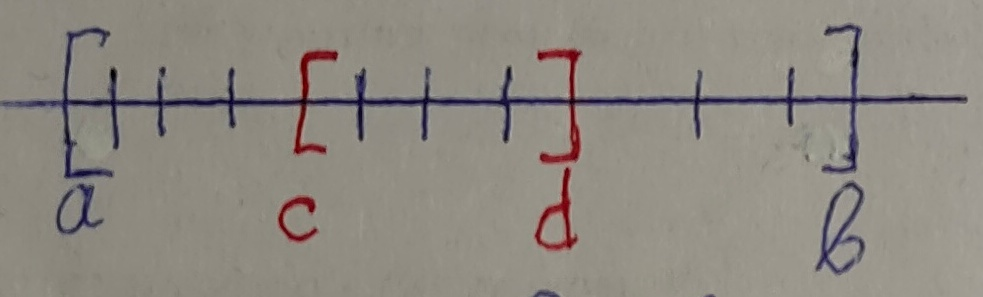
\includegraphics[width=0.2\textwidth]{img/lecture28/scheme_segments}
    	\end{center}
    	\begin{center}
    		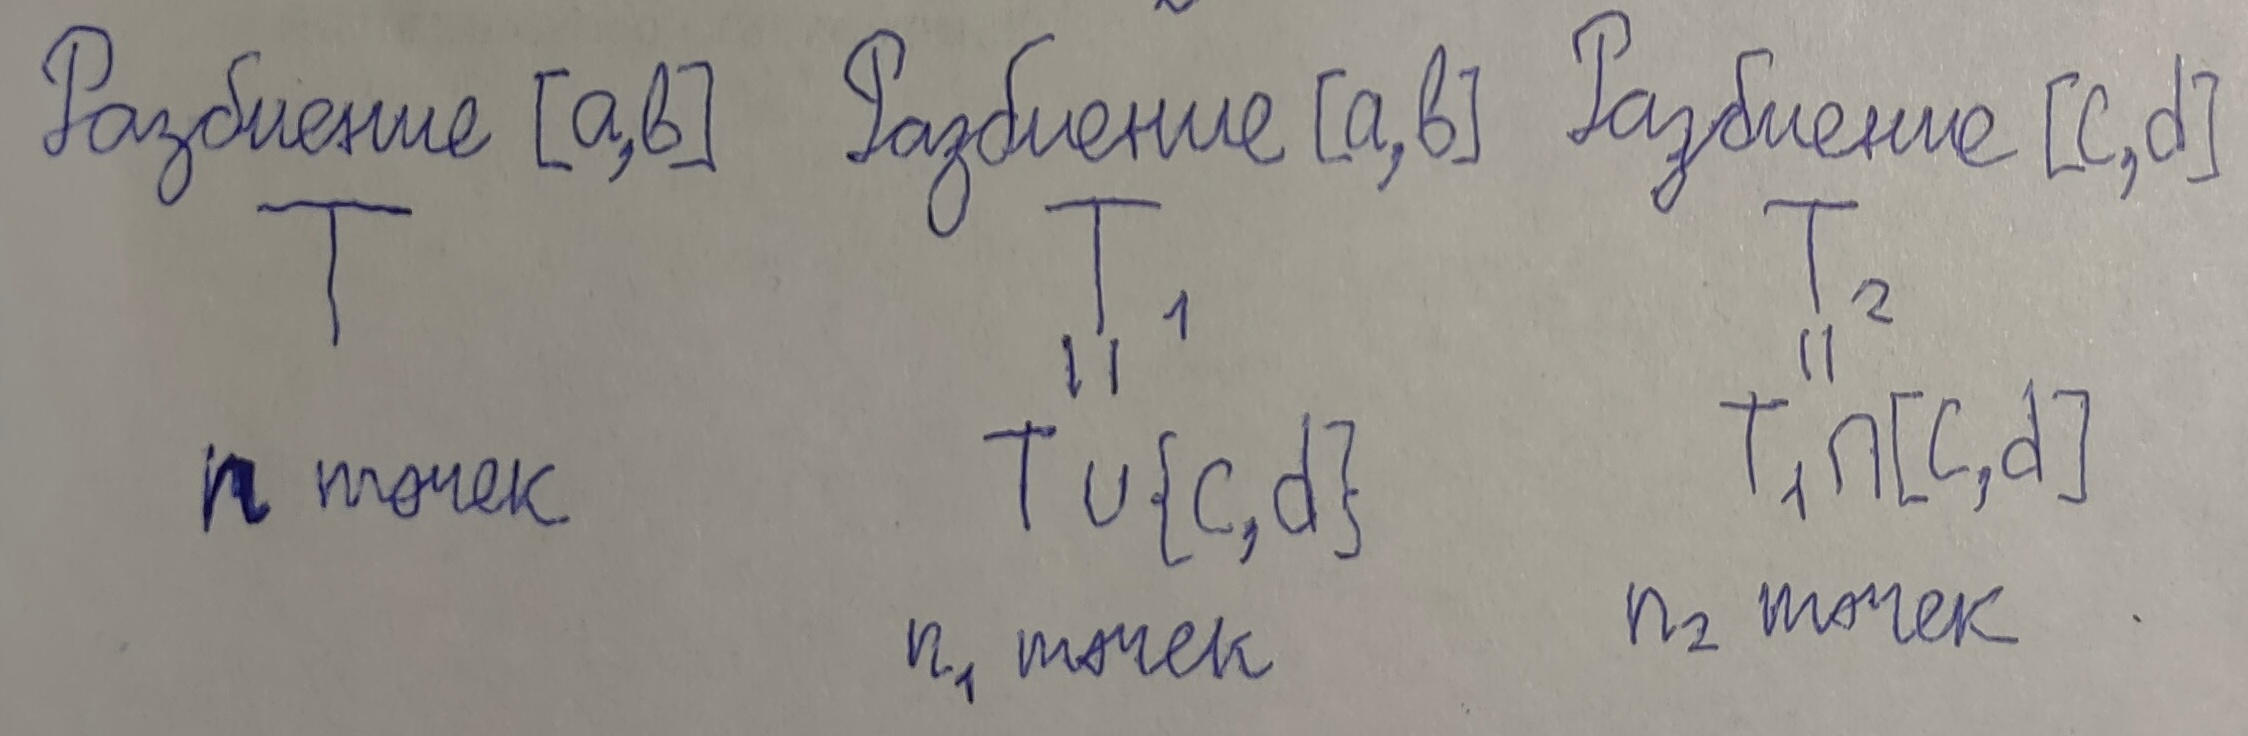
\includegraphics[width=0.5\textwidth]{img/lecture28/partition_designations}
    	\end{center}
    	\[ \sum_{k = 1}^{n_2} \omega(f, \Delta^2_k) \Delta^2 x_k \leqslant \sum_{k = 1}^{n_1} \omega(f, \Delta^1_k) \Delta^1 x_k \leqslant \sum_{k = 1}^n \omega(f, \Delta_k) \Delta x_k < \epsilon \]
    	
    	Первое неравенство выполняется, потому что в новую сумму мы добавили слагаемые отрезков, не входящих в отрезок $[c, d]$, но принадлежащих отрезку $[a, b]$, колебание функции всегда неотрицательно (разность супремума и инфимума функции неотрицательна). Здесь мы переходим от разбиения $T_2$ к разбиению $T_1$. Второе неравенство выполняется, потому что $T_1$ - это измельчение разбиения $T$. На измельчении нижняя сумма Дарбу $s(f, T_1)$ только больше, а верхняя сумма Дарбу $S(f, T_1)$ только меньше, значит разность $S(f, T_1) - s(f, T_1) \leqslant S(f, T) - s(f, T)$ (лемма 10.2, пункт 2).
    \end{proof}
    
    \begin{corollary}
    	Если $f$ интегрируема по Риману на отрезке $[a, b]$, $c \in [a, b]$, то $f$ интегрируема на отрезках $[a, c]$ и $[c, b]$ и верно равенство
    	\[ \int_a^b f(x) \; dx = \int_a^c f(x) \; dx + \int_c^b f(x) \; dx. \]
    \end{corollary}
    
    \begin{proof}
    	Если интеграл слева существует, то существуют и интегралы cправа по предыдущему следствию (на самом деле утверждение верно в обратную сторону, но доказательство на лекциях не приводилось).
    	
    	\begin{mention}
    		Если $f$ - интегрируема на $[a, b]$, то для любой последовательности разбиений $T_n$ такой, что $\Delta_{T_n} \to 0$, интегральная сумма $\sigma(f, T_n, \xi_n) \to I$.
    	\end{mention}
    	\begin{proof}
    		$f$ - интегрируема на $[a, b] \Rightarrow$ по определению $\forall \epsilon > 0 \text{ } \exists \delta > 0: \forall T$ с $\Delta_T < \delta$ и $\xi \rightarrow |\sigma(f, T_n, \xi_n) - I| < \epsilon$
    		
    		Тогда
    		\[ \forall \epsilon > 0 \text{ } \exists N: \forall n > N \text{ } \Delta_{T_n} < \delta \rightarrow |\sigma(f, T_n, \xi_n) - I| < \epsilon \Rightarrow \sigma(f, T_n, \xi_n) \rightarrow I \]
    	\end{proof}
    	
    	Это означает, что если функция интегрируемая, то можно выбирать любое разбиение, с стремящимся к нулю диаметром, чтобы найти интеграл.
    	
    	Будем брать такое разбиение $T$ отрезка $[a, b]$, которые содержат точку $c$. $T_1$ - разбиение отрезка $[a, c]$, $T_2$ - разбиение отрезка $[c, b]$.
    	\begin{center}
    		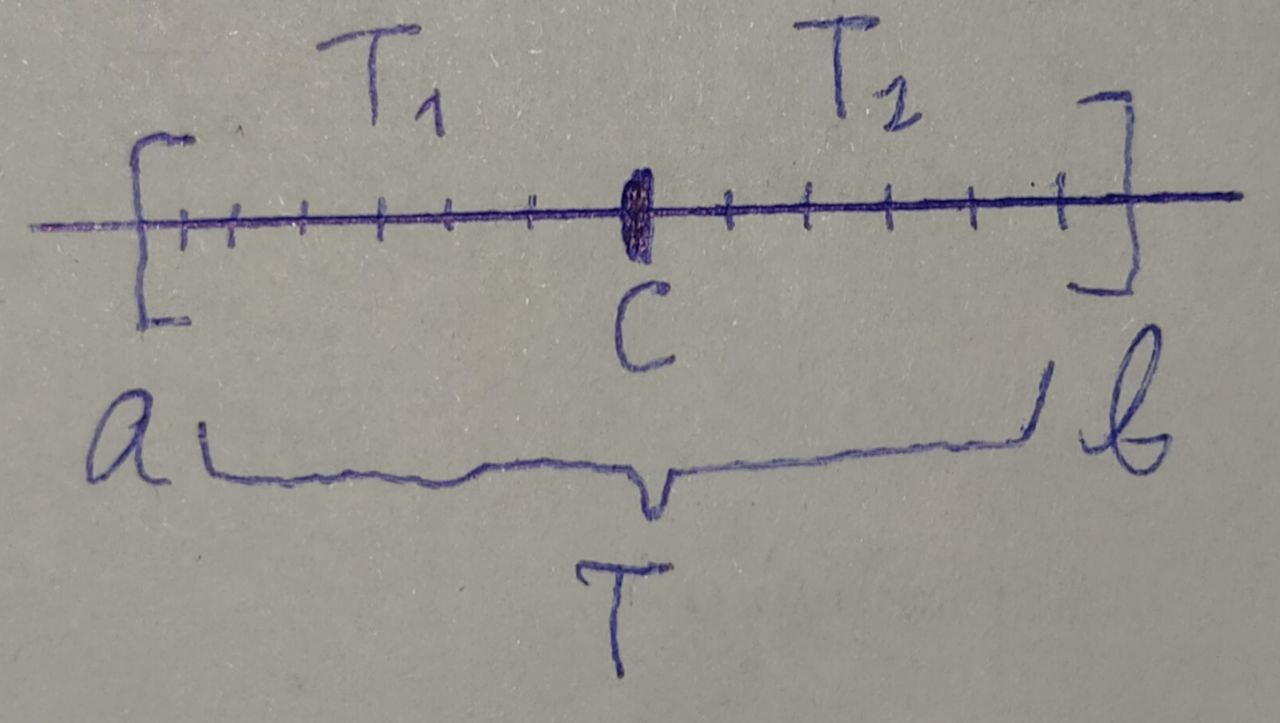
\includegraphics[width=0.3\textwidth]{img/lecture28/partition_with_c_dot}
    	\end{center}
    	
    	$f$ - интегрируема $\Rightarrow \forall \epsilon > 0 \text{ } \exists \delta > 0: \forall T \text{ с } \Delta_T < \delta \rightarrow |\sigma(f, T, \xi) - I| < \epsilon$
    	
    	$\Delta_T < \delta \Rightarrow \Delta_{T_1} < \delta, \Delta_{T_2} < \delta \Rightarrow |\sigma(f, T_1, \xi_1) - I_1| < \epsilon, |\sigma(f, T_2, \xi_2) - I_2| < \epsilon$
    	
    	Пусть отрезок $[a, c]$ поделен на $n_1$ отрезков. Тогда    	
    	\[ \sigma(f, T, \xi) = \sum_{k = 1}^n f(\xi_k) \Delta x_k = \sum_{k = 1}^{n_1} f(\xi_k) \Delta x_k + \sum_{k = n_1 + 1}^n f(\xi_k) \Delta x_k = \sigma(f, T_1, \xi_1) + \sigma(f, T_2, \xi_2) \Rightarrow \]
    	\[ \Rightarrow |\sigma(f, T, \xi) - I_1 - I_2| = |\sigma(f, T_1, \xi_1) + \sigma(f, T_2, \xi_2) - I_1 - I_2| \leqslant \]
    	\[ \leqslant |\sigma(f, T_1, \xi_1) - I_1| + |\sigma(f, T_2, \xi_2) - I_2| < 2\epsilon \]
    	Следовательно,
    	\[ \sigma(f, T, \xi) \to I, \sigma(f, T, \xi) \to I_1 + I_2 \Rightarrow I_1 + I_2 = I \]
    \end{proof}
    
    \section{Формула Ньютона–Лейбница}
    
    \begin{theorem}[Формула Ньютона–Лейбница]
    	Пусть $F$ - первообразная интегрируемой по Риману на отрезке
    	$[a, b]$ функции $f$. Тогда
    	\[ \int_{a}^{b} f(x) \; dx = F(b) - F(a) = F(x)\bigg|_{a}^{b}. \]
    \end{theorem}
    
    \begin{proof}
    	Рассмотрим разбиение $T$ отрезка $[a, b]$.
    	\begin{center}
    		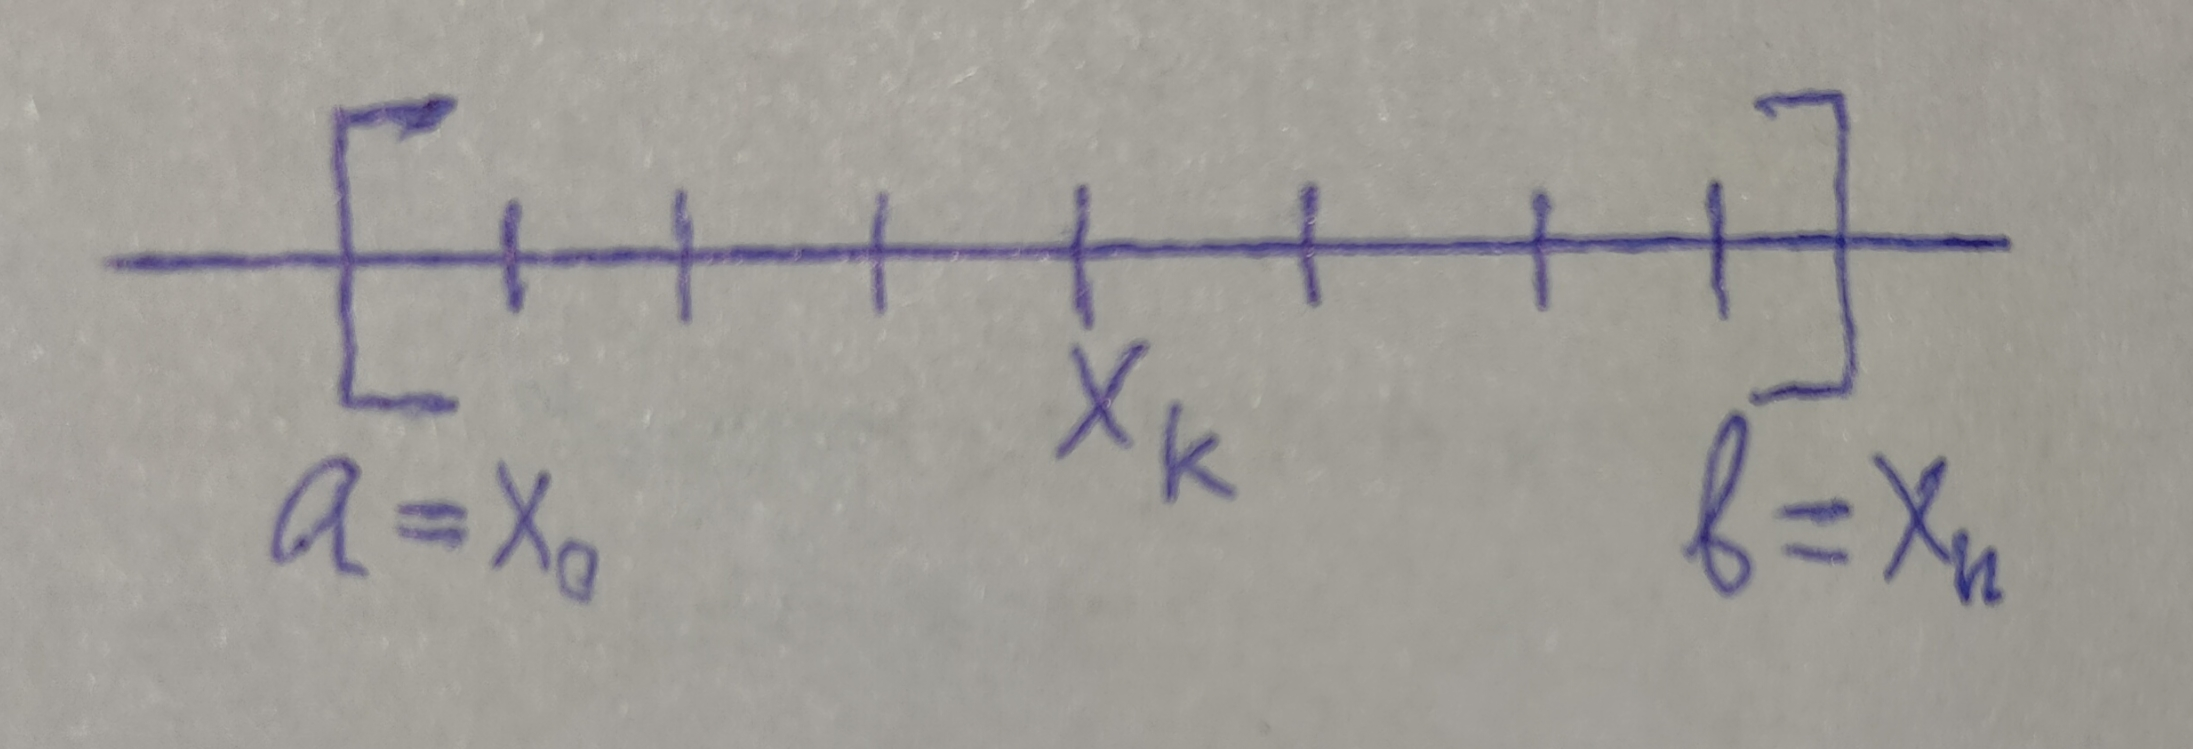
\includegraphics[width=0.3\textwidth]{img/lecture28/Newton_Leibniz_theorem}
    	\end{center}
    	\[ F(b) - F(a) = F(x_1) - F(x_0) + F(x_2) - F(x_1) + F(x_3) - F(x_2) + ... \]
    	\[ ... + F(x_n) - F(x_{n - 1}) = \sum_{k = 1}^n F(x_k) - F(x_{k - 1}) = (*) \]
    	Применяем теорему Лагранжа для каждого отрезка $[x_{k - 1}, x_k]$:
    	\[ (*) = \sum_{k = 1}^n F'(\xi_k) \Delta x_k = \sum_{k = 1}^n f(\xi_k) \Delta x_k = \sigma(f, T, \xi) \]
    	Число $F(b) - F(a)$ равняется интегральной сумме Римана $\sigma(f, T, \xi)$. Поскольку функция интегрируема, то по замечанию из следствия выше при $T \to 0$ интегральная сумма Римана стремится к интегралу $\int_{a}^{b} f(x) \; dx$. При этом, как мы показали, для любого разбиения $T$ всегда есть такая разметка $\xi$, когда $F(b) - F(a) = \sigma(f, T, \xi)$. Тогда
    	\[ \int_{a}^{b} f(x) \; dx = F(b) - F(a) \]
    \end{proof}
    
    Далее будем использовать соглашение: при $b > a$ по
    определению 
    \[ \displaystyle\int_{b}^{a} f(x) \; dx = -\displaystyle\int_{a}^{b} f(x) \; dx.\]
    
    \section{Существование первообразной}
    
    \begin{theorem}
    	Пусть $f$ интегрируема по Риману на $[a, b]$. Тогда функция
    	\[ F(x) := \int_a^{x} f(x) \; dx \]
    	непрерывна на $[a, b]$. Кроме того, если $f$ непрерывна в точке
    	$x_0 \in [a, b]$, то $F$ дифференцируема в $x_0$ и $F'(x_0) = f(x_0)$.
    \end{theorem}
    
    \begin{proof}
    	Доказательство первого утверждения.
    	
    	$y \in [a, b]$    	
    	\[ F(y) = \int_a^y f(x) \; dx \]
    	\[ |F(y) - F(x_0)| = \bigg| \int_a^y f(x) \; dx - \int_a^{x_0} f(x) \; dx \bigg| =  \bigg| \int_{x_0}^y f(x) \; dx \bigg| \]
    	$f$ - интегрируема на $[a, b] \Rightarrow$ ограничена: $|f(x)| \leqslant M$
    	\[  \bigg| \int_{x_0}^y f(x) \; dx  \bigg| \leqslant  \bigg| \int_{x_0}^y M \; dx  \bigg| = M \cdot |y - x_0| \Rightarrow \]
    	$\Rightarrow$ при $y \to x_0$ $F(y) \to F(x_0) \Rightarrow F(x)$ непрерывна.
    	
    	Доказательство второго утверждения.
    	
    	Пусть теперь $f$ непрерывна в $x_0 \Rightarrow \forall \epsilon > 0 \text{ } \exists \delta > 0: \forall x \in B_{\delta}(x_0) \rightarrow |f(x) - f(x_0)| < \epsilon$
    	\[ f(x_0) - \epsilon \leqslant f(x) \leqslant f(x_0) + \epsilon \]
    	Воспользуемся монотонностью интеграла и проинтегрируем каждую часть.
    	\[ \int_{x_0}^x (f(x_0) - \epsilon) \; dx \leqslant \int_{x_0}^x f(x) \; dx \leqslant \int_{x_0}^x (f(x_0) + \epsilon) \; dx \]
    	\[ (f(x_0) - \epsilon)(x - x_0) \leqslant F(x) - F(x_0) \leqslant (f(x_0) + \epsilon)(x - x_0) \]
    	Пусть $x > x_0$, поделим на $x - x_0$.
    	\[ f(x_0) - \epsilon \leqslant \frac{F(x) - F(x_0)}{x - x_0} \leqslant f(x_0) + \epsilon \Rightarrow \bigg| \frac{F(x) - F(x_0)}{x - x_0} - f(x_0) \bigg| < \epsilon \]
    	Это означает, что предел $\lim_{x \to x_0} \frac{F(x) - F(x_0)}{x - x_0}$ существует и он равен $f(x_0)$. Таким образом, $F$ дифференцируема в $x_0$ и $F'(x_0) = f(x_0)$.
    	
    	Если $x < x_0$, то когда поделим на $x - x_0$ знаки перевернутся, но в итоге мы получим тоже самое.
    \end{proof}
    
    \begin{corollary}
    	Пусть $f$ непрерывна на $[a, b]$, тогда у $f$ существует первообразная.
    \end{corollary}
    
    \begin{explanation}
    	Если во всех точках $f$ непрерывна, то по теореме 10.19 первообразная $f$ существует во всех точках.
    \end{explanation}
    
    \section{Формула интегрирования по частям}
    
    \begin{theorem}[Формула интегрирования по частям]
    	Пусть $f$, $g$ — непрерывно дифференцируемые на отрезке $[a, b]$ функции. Тогда
    	\[ \int_a^b f(x)g'(x) \; dx = f(b)g(b) - f(a)g(a) - \int_a^b f'(x)g(x) \; dx. \]
    \end{theorem}
    
    \begin{proof}
    	$F(x) = g(x) \cdot f(x)$
    	
    	$F'(x) = g'(x) \cdot f(x) + g(x) \cdot f'(x)$
    	
    	Непрерывно дифференцируемая функция - это дифференцируемая функция, у которой первая производная непрерывна. Это означает, что $g'(x) \cdot f(x)$ и $g(x) \cdot f'(x)$ непрерывны $\Rightarrow g'(x) \cdot f(x) + g(x) \cdot f'(x)$ непрерывна. У непрерывных функций есть первообразная по предыдущему следствию. Тогда мы можем их интегрировать.
    	
    	$\int_a^b F'(x) \; dx = F(b) - F(a)$    	
    	\[ g(b) \cdot f(b) - g(a) \cdot f(a) = F(b) - F(a) = \int_a^b F'(x) \; dx = \int_a^b g'(x) \cdot f(x) + g(x) \cdot f'(x) \; dx = \]
    	\[ = \int_a^b g'(x) \cdot f(x) \; dx + \int_a^b g(x) \cdot f'(x) \; dx \]
    \end{proof}
    
    \begin{example}
    	$\displaystyle\int_0^1 \arctg{x} \; dx.$
    \end{example}
    \[ \displaystyle\int_0^1 \arctg{x} \; dx = x\arctg{x}\bigg|_0^1 - \int_0^1 x \; d\arctg{x} = \frac{\pi}{4} - \int_0^1 \frac{x}{1 + x^2} \; dx = \frac{\pi}{4} - \frac{1}{2} \int_0^1 \frac{d(1 + x^2)}{1 + x^2} = \]
    \[ = \frac{\pi}{4} - \frac{1}{2} \ln{|x^2 + 1|} \bigg|_0^1 = \frac{\pi}{4} - \frac{\ln{2}}{2} \]
    
    \chapter{Критерий Дарбу и классы интегрируемых функций}
    
    \section*{Лекция 29: Несобственный интеграл}
    
    \section{Формула интегрирования подстановкой}
    
    \begin{theorem}
    	Пусть $f$ — непрерывна на $[a, b], \phi: [\alpha, \beta] \rightarrow [a, b]$ — непрерывно дифференцируемая функция. Тогда
    	\[ \int_{\phi(\alpha)}^{\phi(\beta)} f(x) \; dx = \int_{\alpha}^{\beta} f(\phi(t))\phi'(t) \; dt. \]
    \end{theorem}
    
    \begin{proof}
    	$f$ — непрерывна на $[a, b] \Rightarrow f$ - интегрируема на $[\phi(a), \phi(b)]$ (функция интегрируема на любом подотрезке $[a, b]$) и у $f$ есть первообразная (по теореме 10.19).
    	
    	Тогда у функции $f(\phi(t))\phi'(t)$ тоже есть первообразная $F(\phi(t))$.
    	
    	\[ \int_{\alpha}^{\beta} f(\phi(t))\phi'(t) \; dt = F(\phi(\beta)) - F(\phi(\alpha)) = \int_{\phi(\alpha)}^{\phi{(\beta)}} f(x) \; dx \]
    \end{proof}
    
    \begin{example}
    	$\displaystyle\int_0^{\frac{\pi}{4}} \frac{1}{1 + \cos^2{x}} \; dx.$
    \end{example}
    
    \[ \int_0^{\frac{\pi}{4}} \frac{1}{1 + \cos^2{x}} \; dx = \int_0^{\frac{\pi}{4}} \frac{\frac{1}{\cos^2{x}}}{\frac{1}{\cos^2{x}} + 1} \; dx = (*) \]
    
    \[ \sin^2{x} + \cos^2{x} = 1 \Rightarrow \tg^2{x} + 1 = \frac{1}{\cos^2{x}} \Rightarrow \tg^2{x} = \frac{1}{\cos^2{x}} - 1 \]
    
    Применяем формулу
    \[ (*) = \int_0^{\frac{\pi}{4}} \frac{d\tg{x}}{\tg^2{x} + 2} = \int_{\tg{0}}^{\tg{\frac{\pi}{4}}} \frac{dy}{y^2 + 2} = \int_0^1 \frac{dy}{y^2 + 2} = \frac{1}{\sqrt{2}} \arctg{\frac{y}{\sqrt{2}}} \bigg|_0^1 = \frac{1}{\sqrt{2}} \arctg{\frac{1}{\sqrt{2}}} \]
    
    \section{Мера Жордана (дополнительный материал)}
    Пусть $\Delta$ — параллелепипед в $\R^n$, являющийся декартовым произведением промежутков вида $[a_i, b_i]$, $(a_i, b_i)$, $[a_i, b_i)$ или $(a_i, b_i]$. Мера Жордана параллелепипеда $\Delta$ определяется как
    произведение
    \[ \mu\Delta = \prod_{i = 1}^{n} (b_i - a_i). \]
    
    Для ограниченного множества $E \subset \R^n$ определяются:
    \begin{itemize}
    	\item внешняя мера Жордана
    	\[ \mu^{*}E = \inf{\sum_{k = 1}^{N} \mu \Delta_k}, \text{   } \bigcup_k{\Delta_k} \supset E \]
    	\item внутренняя мера Жордана
    	\[ \mu_{*}E = \sup{\sum_{k = 1}^{N} \mu \Delta_k}, \bigcup_k{\Delta_k} \subset E, \Delta_k \cap \Delta_m = \varnothing, \text{ если } k \neq m. \]
    \end{itemize}
    
    Здесь $\Delta_1, \Delta_2, ..., \Delta_N$ — параллелепипеды описанного выше вида.
    
    \begin{definition}
    	Множество $E$ называется измеримым по Жордану (или
    	квадрируемым), если $\mu^{*}E = \mu_{*}E$. В этом случае мера Жордана равна $\mu E = \mu^{*}E = \mu_{*}E$.
    \end{definition}
    
    \section{Несобственный интеграл Римана}
    
    \begin{definition}
    	Пусть $f$ интегрируема на каждом отрезке $[a, x]$ при $x < b$ $(b \in (-\infty, +\infty])$. Говорят, что несобственный интеграл
    	\[ \int_a^b f(t) \; dt \]
    	\underline{сходится}, если существует предел
    	\[ \lim_{x \to b - 0} \int_a^x f(t) \; dt. \]
    
	    В этом случае значение несобственного интеграла полагают равным значению данного предела. В противном случае (если предела не существует) говорят, что несобственный интеграл \underline{расходится}.
	    
	    Аналогично определяется несобственный интеграл с особенностью в нижнем пределе интегрирования.
	\end{definition}
	
	\begin{example}
	    \begin{equation*}
	    	\int_1^b \frac{1}{x^p} \; dt = 
		    \begin{cases}
		    	\frac{1}{1 - p}(b^{1 - p} - 1), & p \neq 1, \\
		    	\ln{b}, & p = 1.
		    \end{cases}
	    \end{equation*}
	    
	    Предел при $b \rightarrow \infty$ существует тогда и только тогда, когда $p > 1$.
	    
	    С другой стороны,
	    \begin{equation*}
	    	\int_b^1 \frac{1}{x^p} \; dt = 
	    	\begin{cases}
	    		\frac{1}{1 - p}(1 - b^{1 - p}), & p \neq 1, \\
	    		-\ln{b}, & p = 1.
	    	\end{cases}
	    \end{equation*}
	    
	    Предел при $b \rightarrow 0$ существует тогда и только тогда, когда $p < 1$.
	\end{example}
	
	\section{Свойства несобственного интеграла}
	
	\begin{theorem}
		Пусть $f$, $g$ интегрируемы на каждом отрезке $[a, x]$ при $x < b$ и пусть для них определены несобственные интегралы на
		промежутке $[a, b)$. Тогда
		\begin{enumerate}
			\item если $b \in \R$ и $f$ интегрируема на $[a, b]$, то значение несобственного интеграла на промежутке $[a, b)$ совпадает со значением обычного интеграла Римана по отрезку $[a, b]$;
			\item функция $\alpha f + \beta g$ интегрируема в несобственном смысле на промежутке $[a, b)$ и
			\[ \int_a^b (\alpha f + \beta g) \; dx = \alpha \int_a^b f(x) \; dx + \beta \int_a^b g(x) \; dx; \]
			\item если $c \in [a, b)$, то
			\[ \int_a^b f(x) \; dx = \int_a^c f(x) \; dx + \int_c^b f(x) \; dx; \]
		\end{enumerate}
	\end{theorem}
	
	\begin{proof}
		\begin{enumerate}
			\item По определению $\int_a^b f(x) \; dx = \lim_{t \to b-} \int_a^t f(x) \; dx$.
			
			По теореме 10.19 если $F(t) = \int_a^t f(x) \; dx$ интегрируема на $[a, b]$, то $F(t)$ непрерывна на $[a, b] \Rightarrow \lim_{t \to b-} \int_a^t f(x) \; dx = F(b) = \int_a^b f(x) \; dx$.
			\item $\int_a^b \alpha f(x) + \beta g(x) \; dx = \lim_{t \to b-} \int_a^t \alpha f(x) + \beta g(x) \; dx \text{ (здесь уже обычный опреде-}$
			
			$\text{лённый интеграл, применяем линейность)} = \lim_{t \to b-} \alpha \int_a^t f(x) \; dx + \beta \int_a^t g(x) \; dx = \alpha \lim_{t \to b-} \int_a^t f(x) \; dx + \beta \lim_{t \to b-} \int_a^t g(x) \; dx = \alpha \int_a^b f(x) \; dx + \beta \int_a^b g(x) \; dx$
			
			Мы предполагаем, что интегралы $\int_a^b f(x) \; dx$ и $\int_a^b g(x) \; dx$ существуют, тогда существует интеграл  $\int_a^b \alpha f(x) + \beta g(x) \; dx$.
			\item $\int_a^b f(x) \; dx = \lim_{t \to b-} \int_a^t f(x) \; dx = (*)$
			
			При $c \in [a, b)$ для уже определённого интеграла применяем аддитивность:
			
			$(*) = \lim_{t \to b-} \int_a^c f(x) \; dx + \int_c^t f(x) \; dx = \int_a^c f(x) \; dx + \lim_{t \to b-} \int_c^t f(x) \; dx = \int_a^c f(x) \; dx + \int_c^b f(x) \; dx.$
			
			В отличие от пункта 2 здесь равенство выполняется в обе стороны: $\int_a^c f(x) \; dx$ является константой, поэтому предел $\lim_{t \to b-} \int_c^t f(x) \; dx$ существует тогда и только тогда, когда существует $\lim_{t \to b-} \int_a^t f(x) \; dx$.
		\end{enumerate}
	\end{proof}
	
	\section{Формула интегрирования подстановкой}
	
	\begin{theorem}
		Пусть $f$ непрерывна на $[a, b)$ и интегрируема в несобственном смысле, $\phi: [\alpha, \beta) \rightarrow [a, b)$ - непрерывно дифференцируемое отображение, $\phi(\alpha) = a, \phi(t) \rightarrow b$ при $t \rightarrow \beta$. Тогда функция $t \mapsto f(\phi(t))\phi'(t)$ интегрируема в несобственном смысле на промежутке $[\alpha, \beta)$ и
		\[ \int_a^b f(x) \; dx = \int_{\alpha}^{\beta} f(\phi(t))\phi'(t) \; dt. \]
	\end{theorem}
	
	\begin{proof}
		Из условия теоремы знаем, что
		\[ \exists \int_a^b f(x) \; dx = \lim_{y \to b-} \int_a^y f(x) \; dx\]
		
		Рассмотрим следующий интеграл (мы не знаем заранее, существует ли он):
		\[ \int_{\alpha}^{\beta} f(\phi(t)) \phi'(t)\; dt = \lim_{s \to \beta} \int_{\alpha}^s f(\phi(t))\phi'(t) \; dt \]
		
		При этом не важно с какой стороны $s$ стремится к $\beta$ (справа или слева), потому что мы определили интеграл как в случае $\alpha < \beta$, так и в случае $\beta < \alpha$.
		
		Для данного определённого интеграла под пределом действует формула интегрирования заменой (теорема 11.1).
		
		\[ \lim_{s \to \beta} \int_{\alpha}^s f(\phi(t))\phi'(t) \; dt = \lim_{s \to \beta} \int_{\phi(\alpha)}^{\phi(s)} f(x) \; dx \]
		
		$\phi(\alpha) = a, \phi(s) \to b$ при $s \to \beta \Rightarrow$
		\[ \lim_{s \to \beta} \int_{\phi(\alpha)}^{\phi(s)} f(x) \; dx = \lim_{y \to b} \int_a^y f(x) \; dx \]
		что тоже самое, что интеграл в начале доказательства. Значит интеграл $\int_{\alpha}^{\beta} f(\phi(t)) \phi'(t)$ существует и равен $\int_a^b f(x) \; dx$.
	\end{proof}
	
	\section{Формула интегрирования по частям}
	
	\begin{theorem}
		Пусть $f, g$ непрерывно дифференцируемы на $[a, b)$ и существует предел $\displaystyle\lim_{x \to b - 0} f(x)g(x)$. Тогда функции $f'g$ и $fg'$ одновременно интегрируемы или не интегрируемы в несобственном смысле на $[a, b)$ и в случае интегрируемости
		\[ \int_a^b f(t)g'(t) \; dt = \lim_{x \to b - 0} f(x)g(x) - f(a)g(a) - \int_a^b f'(t)g(t) \; dt. \]
	\end{theorem}
	
	\begin{proof}
		Если существует $\displaystyle\lim_{x \to b - 0} f(x)g(x)$, то $\displaystyle\lim_{x \to b - 0} f(x)g(x) - f(a)g(a)$ - это число. Тогда функции $f'g$ и $fg'$ одновременно интегрируемы или не интегрируемы в несобственном смысле на $[a, b)$.
		
		В случае интегрируемости
		\[ \int_a^b f(t)g'(t) \; dt = \lim_{x \to b} \int_a^x f(t)g'(t) \; dt \]
		Применяем формулу интегрирования по частям для определённого интеграла
		\[ \lim_{x \to b} \int_a^x f(t)g'(t) \; dt = \lim_{x \to b-} \bigg(f(x)g(x) - f(a)g(a) - \int_a^x f'(t)g(t) \; dt \bigg) = \]
		\[ = \lim_{x \to b-} f(x)g(x) - f(a)g(a) - \int_a^b f'(t)g(t) \; dt \]
	\end{proof}
	
	\section{Критерий Коши}
	
	\begin{theorem}[Критерий Коши]
		Пусть функция $f(x)$ определена на промежутке $[a; b)$,
		интегрируема в собственном смысле на любом отрезке
		$[a; \xi] \subseteq [a; b)$ и неограниченна в левой окрестности точки $x = b$. Тогда для сходимости интеграла
		\[ \int_a^b f(x) \; dx \]
		необходимо и достаточно, чтобы для любого числа $\epsilon > 0$
		существовало такое число $\eta$, что при любых $\eta_1, \eta_2 \in (\eta; b)$
		\[ \bigg| \int_{\eta_1}^{\eta_2} f(x) \; dx \bigg| < \epsilon. \]
	\end{theorem}
	
	\begin{proof}
		Запишем критерий Коши для функции $F(x) = \int_a^x f(t) \; dt$:
		\[ \exists \lim_{x \to b-} F(x) \Leftrightarrow \forall \epsilon > 0 \text{ } \exists \delta = \eta > 0 \text{ } \forall \eta_1, \eta_2 \in B_{\delta}(b) \rightarrow |F(\eta_1) - F(\eta_2)| < \epsilon \Rightarrow \]
		\[ \Rightarrow \bigg| \int_{a}^{\eta_1} f(x) \; dx - \int_{a}^{\eta_2} f(x) \; dx \bigg| = \bigg| \int_{a}^{\eta_1} f(x) \; dx + \int_{\eta_2}^{a} f(x) \; dx \bigg| = \bigg| \int_{\eta_2}^{\eta_1} f(x) \; dx \bigg| = \]
		\[ = \bigg| \int_{\eta_1}^{\eta_2} f(x) \; dx \bigg| < \epsilon \]
	\end{proof}
	
	\section*{Лекция 30: Абсолютная сходимость}
	
	\section{Абсолютная сходимость}
	
	\begin{definition}
		Говорят, что несобственный интеграл $\displaystyle \int_a^b f(t) \; dt$ сходится \textbf{абсолютно}, если сходится интеграл $\displaystyle \int_a^b |f(t)| \; dt$.
	\end{definition}
	
	\begin{sentence}
		Из абсолютной сходимости интеграла следует обычная сходимость.
	\end{sentence}
	
	\begin{proof}
		Запишем критерий Коши (теорема 11.9)
		\[ \int_a^b |f(x)| \; dx \text{ - сходится} \Leftrightarrow \forall \epsilon > 0 \text{ } \exists \delta > 0: \eta_1, \eta_2 \in B_{\delta}(b) \rightarrow \bigg| \int_{\eta_1}^{\eta_2} |f(x)| \; dx \bigg| < \epsilon \]
		
		Применяем замечание 9.8 (первое неравенство)
		\[ \bigg| \int_{\eta_1}^{\eta_2} f(x) \; dx \bigg| \leqslant \int_{\eta_1}^{\eta_2} |f(x)| \; dx \leqslant \bigg| \int_{\eta_1}^{\eta_2} |f(x)| \; dx \bigg| < \epsilon \]
		Значит сходится интеграл $\displaystyle \int_a^b f(t) \; dt$.
	\end{proof}
	
	\begin{mention}
		Исследование абсолютной сходимости сводится к исследованию сходимости интеграла от неотрицательной функции. В случае неотрицательной функции $f$ функция $F$ оказывается монотонной, поэтому сходимость интеграла от неотрицательной функции равносильна ограниченности $F$ на $[a, b)$ (применяем теорему Вейерштрасса).	
	\end{mention}
	
	\section{Условная сходимость}
	
	\begin{definition}
		Говорят, что несобственный интеграл $\int_a^b f(t) \; dt$ сходится \textbf{условно}, если сам интеграл сходится, но не сходится
		абсолютно.
	\end{definition}
	
	\begin{example}
		Примером условно сходящегося интеграла может служить интеграл $\displaystyle \int_1^{\infty} \frac{\sin{x}}{x} \; dx$.
    \end{example}
    
    \begin{proof}
		Формула интегрирования по частям дает следующее равенство
		\[ \int_1^{\infty} \frac{\sin{x}}{x} \; dx = -\frac{\cos{x}}{x} \bigg|_1^{\infty} - \int_1^{\infty} \frac{\cos{x}}{x^2} \; dx, \]
		Последний интеграл в этом равенстве сходится абсолютно, поскольку
		\[ \int_1^{\infty} \bigg|\frac{\cos{x}}{x^2}\bigg| \; dx \leqslant \int_1^{\infty} \bigg|\frac{1}{x^2}\bigg| \; dx \text{ - сходится.} \]
		В то же время, $\displaystyle \int_1^{\infty} \frac{\sin{x}}{x} \; dx$ не сходится абсолютно. Действительно,
		\[ \int_1^{\infty} \bigg|\frac{\sin{x}}{x}\bigg| \; dx \geqslant \int_1^{\infty} \frac{\sin^2{x}}{x} \; dx = \int_1^{\infty} \frac{1}{2x} - \frac{\cos{2x}}{2x} \; dx \text{ (формула: } 2\sin^2{x} = 1 - \cos{2x}) \]
		Первый интеграл в последнем равенстве расходится, а второй, как и выше, равен
		\[ \int_1^{\infty} \frac{\cos{x}}{x} \; dx = \frac{\sin{x}}{x} \bigg|_1^{\infty} + \int_1^{\infty} \frac{\sin{x}}{x^2} \; dx \text{ - сходится.} \]
		Это означает, что $\displaystyle \int_1^{\infty} \bigg|\frac{\sin{x}}{x}\bigg| \; dx$ является суммой сходящегося и расходящегося интеграла и, следовательно, расходится.
	\end{proof}
	
	\section{Несобственный интеграл от знакопостоянной функции}
	
	\begin{theorem}[Критерий сходимости несобственного
		интеграла от знакопостоянной функции]
		Пусть функция $f(x) \geqslant 0$ интегрируема на любом отрезке
		$[a, b'] \subset [a, b)$. Тогда сходимость интеграла $\displaystyle \int_a^b f(x) \; dx$	эквивалентна условию $\displaystyle \sup_{b' \in [a, b)} {\int_a^{b'} f(x) \; dx < +\infty}$.
	\end{theorem}
	
	\begin{proof}
		Рассмотрим функцию $F(y) = \int_a^y f(x) \; dx$. На любом отрезке $[x_1, x_2] \subset [a, b)$ функция $f(x)$ интегрируема (в силу следствия 10.15) и, поскольку $f(x) \geqslant 0, F(y)$ - монотонна:
		\[ F(x_2) = \int_a^{x_2} f(x) \; dx = \int_a^{x_1} f(x) \; dx + \int_{x_1}^{x_2} f(x) \; dx \geqslant  \int_a^{x_1} f(x) \; dx = F(x_1). \]
		Тогда, в силу теоремы Вейерштраса 3.18, если $F(y)$ - ограничена, то
		\[ \sup_{y \in [a, b]} F(y) = \lim_{y \to b} \int_a^y f(x) \; dx = \int_a^b f(x) \; dx. \]
		В обратную сторону
		\[ \exists \int_a^b f(x) \; dx = \lim_{y \to b} \int_a^y f(x) \; dx \Rightarrow F(x) - \text{ограничена.} \]
	\end{proof}
	
	\section{Первый признак сравнения}
	
	\begin{theorem}[Первый признак сравнения]
		Пусть функции $f(x)$ и $g(x)$ интегрируемы на любом отрезке
		$[a, b'] \subset [a, b)$ и для любого $x \in [a, b)$ $0 \leqslant f(x) \leqslant g(x)$. Тогда:
		\begin{itemize}
			\item из сходимости $\displaystyle \int_a^b g(x) \; dx$ следует сходимость $\displaystyle \int_a^b f(x) \; dx$;
			\item из расходимости $\displaystyle \int_a^b f(x) \; dx$ следует расходимость $\displaystyle \int_a^b g(x) \; dx.$
		\end{itemize}
	\end{theorem}
	
	\begin{proof}
		Поскольку $0 \leqslant f(x) \leqslant g(x)$, из монотонности интеграла 9.7 следует, что для любого $y \in [a, b)$:
		\[ 0 \leqslant \int_a^y f(x) \; dx \leqslant \int_a^y g(x) \; dx. \]
		
		Если $\int_a^b g(x) \; dx$ сходится, то по критерию сходимости несобственного интеграла от знакопостоянной функции 11.15 функция $G(y) = \int_a^y g(x) \; dx$ — ограничена. Тогда из неравенства выше следует, что и функция $F(y) = \int_a^y f(x) \; dx$ ограничена. Отсюда, в силу теоремы 11.15, следует сходимость интеграла $\int_a^b f(x) \; dx$.
		
		Если же $\int_a^b f(x) \; dx$ расходится, то $F(y)$ неограничена, как и функция $G(y)$.
	\end{proof}
	
	\section{Эквивалентность в смысле сходимости интегралов}
	
	\begin{definition}
		Будем говорить, что $f(x)$ и $g(x)$ эквивалентны в смысле
		сходимости интегралов при $x \rightarrow b - 0$ (обозн. $f(x) \overset{\text{сх.}}{\sim} g(x)$ при $x \rightarrow b - 0$), если $\exists m, M > 0, b_1 < b$ такие, что $\forall x \in [b_1, b)$ выполняются неравенства
		\[ mg(x) \leqslant f(x) \leqslant Mg(x).\]
	\end{definition}
	
	\begin{theorem}[Второй признак сравнения]
		Пусть неотрицательные функции $f(x)$ и $g(x)$ интегрируемы на
		любом отрезке $[a, b'] \subset [a, b)$ и $f(x) \overset{\text{сх.}}{\sim} g(x)$ при $x \rightarrow b - 0$.
		
		Тогда несобственные интегралы $\int_a^b g(x) \; dx$ и $\int_a^b f(x) \; dx$ сходятся и расходятся одновременно.
	\end{theorem}
	
	\begin{proof}
		Функции эквивалентны в терминах сходимости, когда $\exists b_1 : \forall x \in [b_1, b)$ для которых выполнено $mg(x) \leqslant f(x) \leqslant Mg(x)$. Тогда
		\[ \int_a^b f(x) \; dx = \int_a^{b_1} f(x) \; dx + \int_{b_1}^b f(x) \; dx \text{ и } \int_a^b g(x) \; dx = \int_a^{b_1} g(x) \; dx + \int_{b_1}^b g(x) \; dx. \]
	    При этом $\int_a^{b_1} f(x) \; dx$ и $\int_a^{b_1} g(x) \; dx$ - определенный интегралы, не влияющие на сходимость. 
	    
	    Исследуем интегралы $\int_{b_1}^b f(x) \; dx$ и $\int_{b_1}^b g(x) \; dx$. Если $\int_{b_1}^b g(x) \; dx$ сходится, то сходится и интеграл $\int_{b_1}^b M g(x) \; dx = M \int_{b_1}^b g(x) \; dx$. Тогда по первому признаку сравнения 11.16 интеграл $\int_{b_1}^b f(x) \; dx$ тоже сходится.
	    
	    И наоборот, если $\int_{b_1}^b g(x) \; dx$ расходится, то расходится и $\int_{b_1}^b m g(x) \; dx = m \int_{b_1}^b g(x) \; dx$. Тогда по первому признаку сравнения 11.16 интеграл $\int_{b_1}^b f(x) \; dx$ тоже расходится.
	\end{proof}
	
	\section{Второй признак сравнения}
	
	\begin{sentence}
		Если $f \geqslant 0$ и $f(x) \sim g(x)$ при $x \rightarrow b - 0$, то $f(x) \overset{\text{сх.}}{\sim} g(x)$.
	\end{sentence}
	
	\begin{proof}
		$g(x) \sim f(x)$ при $x \to b - 0 \Leftrightarrow \lim_{x \to b} \frac{f(x)}{g(x)} = 1$. Тогда $\exists \delta: \forall x \in B'_\delta(b):$
		\[ \bigg|\frac{f(x)}{g(x)} - 1\bigg| < \frac{1}{2}. \]
		Отсюда
		\[ \frac{1}{2} < \frac{f(x)}{g(x)} < \frac{3}{2}. \]
		Тогда $g(x) > 0$ и
		\[ \frac{1}{2} g(x) < f(x) < \frac{3}{2} g(x). \]
	\end{proof}
	
	\begin{sentence}
		Пусть $f_i(x), g_i(x)$ $i \in \{1, 2, 3\}$ - неотрицательные на
		промежутке $[a, b)$ функции, причем $f_3(x) > 0, g_3(x) > 0$ и
		$f_i(x) \overset{\text{сх.}}{\sim} g_i(x)$ $i \in \{1, 2, 3\}$ при $x \rightarrow b - 0$. Тогда
		\[ \frac{f_1(x) \cdot f_2(x)}{f_3(x)} \overset{\text{сх.}}{\sim} \frac{g_1(x) \cdot g_2(x)}{g_3(x)} \text{ при } x \rightarrow b - 0.\]
	\end{sentence}
	
	\begin{proof}
		????????????????
	\end{proof}
	
	\begin{example}
		Исследовать на сходимость $\displaystyle \int_1^{+\infty} \frac{\arctan{\frac{1}{x}}\sin{(\frac{2 + \cos{x}}{x^2})}}{(e^{\frac{1}{x}} - 1)^{\alpha}} \; dx$.
	\end{example}
	
	\section*{Лекция 31: Еще немного про числовые ряды}

	\section{Первый признак сравнения}
	
	\begin{definition}
		Ряд $\sum_{n = 1}^{\infty} a_n$ называется \textbf{знакопостоянным}, если или
		$a_n \geqslant 0 \text{ } \forall n \in \N$, или $a_n \leqslant 0 \text{ } \forall n \in \N$.
	\end{definition}
	
	\begin{sentence}[Первый признак сравнения]
		Пусть $0 \leqslant a_n \leqslant b_n$. Если ряд $\displaystyle \sum_{k = 1}^{\infty} b_k$ сходится, то сходится и ряд $\displaystyle \sum_{k = 1}^{\infty} a_k$. Наоборот, если ряд $\displaystyle \sum_{k = 1}^{\infty} a_k$ расходится, то расходится и ряд $\displaystyle \sum_{k = 1}^{\infty} b_k$.
	\end{sentence}
	
	Было доказано ранее.
	
	\begin{mention}
		Поскольку первые несколько членов не влияют на сходимость ряда, достаточно, чтобы неравенства выше выполнялись начиная с некоторого момента $\forall n > n_0$. Это называется \textbf{принципом локализации}.
	\end{mention}
	
	\begin{corollary}[Признак Вейерштрасса]
		Если $|a_n| \leqslant b_n$ и ряд $\displaystyle \sum_{n = 1}^{\infty} b_n$ сходится, то ряд $\displaystyle \sum_{n = 1}^{\infty} a_n$ сходится.
	\end{corollary}
	
	\begin{proof}
		Ряд $\sum_{k = 1}^{\infty} |a_n|$ сходится по первому признаку сравнения. Если ряд сходится абсолютно, то он и просто сходится.
	\end{proof}
	
	\section{Второй признак сравнения}
	
	\begin{theorem}[Второй признак сравнения]
		Пусть $a_n, b_n > 0$ и $\displaystyle \exists \lim_{n \to \infty} {\frac{a_n}{b_n}} = c \neq 0$. Тогда $\displaystyle \sum_{n = 1}^{\infty} a_n \sim \sum_{n = 1}^{\infty} b_n -$ эквивалентны по сходимости, т.е. сходятся/расходятся одновременно.
	\end{theorem}
	
	\begin{proof}
		$\lim_{n \to \infty} \frac{a_n}{b_n} = c \neq 0 \Rightarrow$ из определения предела следует, что $\exists n \geqslant N \rightarrow \frac{1}{2} c \leqslant \frac{a_n}{b_n} \leqslant \frac{3}{2} c$ (отступили на $\frac{1}{2}c$ обе стороны) $\Rightarrow \frac{1}{2} c \cdot b_n \leqslant a_n \leqslant \frac{3}{2} c \cdot b_n$
		
		$c$ - положительное число, поэтому можно применять первый признак сравнения.
		
		\begin{enumerate}
			\item $\sum_{n = 1}^{\infty} a_n$ - расходится $\Rightarrow \sum_{n = 1}^{\infty} \frac{3}{2} c \cdot b_n$ - расходится (по первому признаку сравнения) $\Rightarrow \frac{3}{2} c \sum_{n = 1}^{\infty} b_n$ - расходится $\Rightarrow \sum_{n = 1}^{\infty} b_n$ - расходится.
			\item $\sum_{n = 1}^{\infty} a_n$ - сходится $\Rightarrow \sum_{n = 1}^{\infty} \frac{1}{2} c \cdot b_n$ - сходится (по первому признаку сравнения) $\Rightarrow \sum_{n = 1}^{\infty} b_n$ - сходится.
		\end{enumerate}
	\end{proof}
	
	\begin{example}
		Теперь мы можем ответить на вопрос, сходится ли ряд $\sum_{n = 1}^{\infty} \arctg{\frac{1}{n^2}}$, т. к. $\arctg{\frac{1}{n^2}} \sim \frac{1}{n^2}$.
	\end{example}
	
	\begin{corollary}
		Если $a_n \geqslant 0$ и $a_n \sim b_n, n \rightarrow \infty,$ то $\displaystyle \sum_{n = 1}^{\infty} a_n \sim \sum_{n = 1}^{\infty} b_n$.
	\end{corollary}
	
	\begin{proof}
		Определение эквивалентности для функций:
		$f(x) \sim g(x)$ при $x \to x_0 \Leftrightarrow \lim_{x \to x_0} \frac{f(x)}{g(x)} = 1$
		
		В частности верно для функций от $n$: 
		$a_n \sim b_n$ при $n \to \infty \Leftrightarrow \lim_{n \to \infty} \frac{a_n}{b_n} = 1 \neq 0$
		
		По предыдущей теореме получаем требуемое.
	\end{proof}
	
	\section{Интегральный признак}
	
	\begin{sentence}
		Пусть $f(x) \geqslant 0$ и не возрастает на промежутке $[1, +\infty)$. Тогда ряд $\displaystyle \sum_{n = 1}^{\infty} f(n)$ и интеграл $\displaystyle \int_1^{+\infty} f(x) \; dx$ сходятся и расходятся одновременно. 
	\end{sentence}
	
	\begin{proof}
		Обозначим через $\displaystyle S_n = \sum_{k = 1}^n f(k)$ частичную сумму ряда $\displaystyle \sum_{k = 1}^{\infty} f(k)$. Поскольку $f(x) \geqslant 0$, последовательность $S_n$ монотонно возрастает.
		
		Заметим, что $\forall b > 1$ функция $f(x)$ интегрируема на любом отрезке $[1, b]$, поскольку $f(x)$ монотонна (следствие 10.9). Также заметим, что в силу монотонности $f(x)$ для $x \in [n, n + 1]$ выполнено
		\[ f(n) \geqslant f(x) \geqslant f(n + 1). \]
		Тем самым, $\forall n \in \N$ выполнено
		\[ \int_n^{n + 1} f(n) \; dx = f(n)((n + 1) - n) = f(n) \geqslant \int_n^{n + 1} f(x) \; dx \geqslant f(n + 1) = \]
		\[ =  f(n + 1)((n + 1) - n) = \int_n^{n + 1} f(n + 1) \; dx. \]
		Отсюда, если $\int_1^{+\infty} f(x) \; dx$ сходится, то
		\[ S_n - f(1) = f(2) + ... + f(n) \leqslant \int_1^n f(x) \; dx \leqslant \int_1^{+\infty} f(x) \; dx < +\infty, \]
		что означает ограниченность $S_n$ и, в силу монотонности $S_n$ и теоремы Вейерштрасса 2.14, сходимость ряда $\displaystyle \sum_{k = 1}^{\infty} f(k)$.
		
		Если же $\int_1^{+\infty} f(x) \; dx$ расходится, то $\displaystyle \lim_{n \to \infty} \int_1^n f(x) \; dx = +\infty$, и
		\[ S_n = f(1) + ... + f(n) \geqslant \int_n^{n + 1} f(x) \; dx \to +\infty, \]
		что означает расходимость ряда $\displaystyle \sum_{k = 1}^{\infty} f(k)$.
	\end{proof}
	
	\begin{example}
		Ряд $\displaystyle \sum_{n = 1}^{\infty} \frac{1}{n^p}$ сходится при $p > 1$ и расходится при $p \leqslant 1$.
	\end{example}
	
	Применяя интегральный признак,
	\[ \sum_{n = 1}^{\infty} \frac{1}{n^p} - \text{сходится} \Leftrightarrow \int_1^{\infty} \frac{1}{x^p} \; dx - \text{сходится} \Leftrightarrow p > 1 \]
	
	\section{Признак Даламбера}
	
	\begin{theorem}[Признак Даламбера]
		Пусть $a_k > 0$ $\forall k \in \N$. Тогда
		\begin{enumerate}
			\item если существует $k_0 \in \N$ и $q \in (0, 1)$ такие, что $\frac{a_{k + 1}}{a_k} \leqslant q$ $\forall k \geqslant k_0,$ то ряд $\displaystyle \sum_{k = 1}^{\infty} a_k$ сходится;
			\item если $\exists k_0 : \forall k \geqslant k_0 \rightarrow \frac{a_{k + 1}}{a_k} \geqslant 1$, то ряд $\displaystyle \sum_{k = 1}^{\infty} a_k$ расходится.
		\end{enumerate}
	\end{theorem}
	
	\begin{proof}
		\begin{enumerate}
			\item Знаем, что ряд $\sum_{k = 1}^{\infty} q^n$ сходится при $|q| < 1$
			
			Пусть $\frac{a_{k + 1}}{a_k} \leqslant q < 1 \text{ } \forall k \geqslant k_0$
			
			\[ a_{k + 1} = \frac{a_{k + 1}}{a_k} \cdot a_k = \frac{a_{k + 1}}{a_k} \cdot \frac{a_k}{a_{k - 1}} \cdot a_{k - 1} = \frac{a_{k + 1}}{a_k} \cdot \frac{a_k}{a_{k - 1}} \cdot ... \cdot \frac{a_{k_0 + 1}}{a_{k_0}} \cdot a_{k_0} \leqslant q^{k - k_0 + 1} a_{k_0} \Leftrightarrow \]
			\[ \Leftrightarrow a_k \leqslant q^{k - k_0} a_{k_0} \Rightarrow \sum_{k = k_0}^{\infty} a_k \leqslant \sum_{k = k_0}^{\infty} q^{k - k_0} a_{k_0} \Rightarrow \text{ряд } \sum_{k = k_0}^{\infty} q^{k - k_0} a_{k_0} \text{ сходится} \Leftrightarrow \]
			\[ \Leftrightarrow \sum_{k = k_0}^{\infty} a_k \text{ сходится (по первому признаку сравнения)} \]
			
			Значит по принципу локализации ряд $\sum_{k = 1}^{\infty} a_k$ - сходится.
			
			\item $\frac{a_{k + 1}}{a_k} \geqslant 1 \Rightarrow a_{k + 1} \geqslant a_k \geqslant ... \geqslant a_{k_0} > 0 \Rightarrow a_k \not\rightarrow 0$, т. е. не выполнено необходимое условие сходимости ряда.
			
		\end{enumerate}
	\end{proof}
	
	\begin{corollary}[Признак Даламбера в предельной форме]
		Пусть $a_k > 0$ $\forall k \in \N$ и $\displaystyle \lim_{k \to \infty} {\frac{a_{k + 1}}{a_k}} = q$, тогда
		
		\begin{enumerate}
			\item при $q < 1$ ряд $\displaystyle \sum_{k = 1}^{\infty} {a_k}$ сходится;
			\item при $q > 1$ ряд $\displaystyle \sum_{k = 1}^{\infty} {a_k}$ расходится;
			\item при $q = 1$ ряд $\displaystyle \sum_{k = 1}^{\infty} {a_k}$ может сходится, а может и расходится.
		\end{enumerate}
	\end{corollary}
	
	\begin{proof}
		\begin{enumerate}
			\item Пусть $q < 1$. Возьмём $q' = \frac{q + 1}{2}$ - середина отрезка $[q, 1]$.
			
			Поскольку $\lim_{n \to \infty} \frac{a_{n + 1}}{a_n} = q$, то 
			\[ \exists N: \forall n > N \rightarrow \frac{a_{n + 1}}{a_n} < q' < 1 \Rightarrow \]
			по признаку Даламбера ряд $\sum_{n = 1}^{\infty} a_n$ - сходится.
			
			\item $q > 1 \Rightarrow \lim_{n \to \infty} \frac{a_{n + 1}}{a_n} = q > 1 \Rightarrow \exists N: \forall n \geqslant N \rightarrow \frac{a_{n + 1}}{a_n} \geqslant 1 \Rightarrow$
			
			по признаку Даламбера ряд $\sum_{n = 1}^{\infty} a_n$ - расходится.
			
			\item $q = 1$. Пример: $a_n = (\frac{1}{n})^p$, ряд $\sum_{n = 1}^{\infty} a_n$.
			\[ \lim_{n \to \infty} \frac{a_{n + 1}}{a_n} = \lim_{n \to \infty} \bigg(\frac{n}{n + 1}\bigg)^p = \lim_{n \to \infty} \bigg(1 - \frac{1}{n + 1}\bigg)^p = 1 \text{ при любом } p \]
			Но ряд $\sum_{n = 1}^{\infty} (\frac{1}{n})^p$ сходится при $p > 1$ и не сходится $p \leqslant 1$.
		\end{enumerate}
	\end{proof}
	
	\section{Радикальный признак Коши}
	
	\begin{theorem}[Радикальный признак Коши]
		Пусть $a_k > 0$ $\forall k \in \N$. Тогда
		\begin{enumerate}
			\item если существуют $k_0 \in \N$ и $q \in (0, 1)$ такие, что $\sqrt[k]{a_k} \leqslant q$ $\forall k \geqslant k_0$, то ряд $\displaystyle \sum_{k = 1}^{\infty} {a_k}$ сходится;
			\item если $\exists k_0: \forall k \geqslant k_0 \rightarrow \sqrt[k]{a_k} \geqslant 1$, то ряд $\displaystyle \sum_{k = 1}^{\infty} {a_k}$ расходится.
		\end{enumerate}
	\end{theorem}
	
	\begin{proof}
		\begin{enumerate}
			\item Пусть $\sqrt[k]{a_k} \leqslant q < 1 \Rightarrow a_k \leqslant q^k \text{ } \forall k > k_0$.
			
			Ряд $\sum_{k = 1}^{\infty} q^k$ - сходится, т. к. $q \in (0, 1) \Rightarrow$ по первому признаку сравнения $\sum_{k = 1}^{\infty} a_k$ - сходится.
			\item $\sqrt[k]{a_k} \geqslant 1 \Rightarrow a_k \geqslant 1 \text{ } \forall k \geqslant k_0 \Rightarrow a_n \not\rightarrow 0 \Rightarrow$ ряд $\sum_{k = 1}^{\infty} a_k$ - расходится в силу необходимого условия сходимости ряда.
		\end{enumerate}
	\end{proof}
	
	\begin{corollary}[Признак Коши в предельной форме]
		Пусть $a_k > 0$ $\forall k \in \N$ и $\displaystyle \lim_{k \to \infty} {\sqrt[k]{a_k}} = q$, тогда
		
		\begin{enumerate}
			\item при $q < 1$ ряд $\displaystyle \sum_{k = 1}^{\infty} {a_k}$ сходится;
			\item при $q > 1$ ряд $\displaystyle \sum_{k = 1}^{\infty} {a_k}$ расходится;
			\item при $q = 1$ ряд $\displaystyle \sum_{k = 1}^{\infty} {a_k}$ может сходится, а может и расходится.
		\end{enumerate}
	\end{corollary}
	
	\begin{proof}
		\begin{enumerate}
			\item Пусть $q < 1$. Возьмём $q' = \frac{q + 1}{2}$ - середина отрезка $[q, 1]$.
			
			Поскольку $\lim_{n \to \infty} \sqrt[n]{a_n} = q$, то 
			\[ \exists N: \forall n > N \rightarrow \sqrt[n]{a_n} < q' < 1 \Rightarrow \]
			по признаку Коши ряд $\sum_{n = 1}^{\infty} a_n$ - сходится.
			
			\item $q > 1 \Rightarrow \lim_{n \to \infty} \sqrt[n]{a_n} = q > 1 \Rightarrow \exists N: \forall n \geqslant N \rightarrow \sqrt[n]{a_n} \geqslant 1 \Rightarrow$
			
			по признаку Даламбера ряд $\sum_{n = 1}^{\infty} a_n$ - расходится.
			
			\item $q = 1$. Пример: $a_n = (\frac{1}{n})^p$, ряд $\sum_{n = 1}^{\infty} a_n$.
			\[ \lim_{n \to \infty} \sqrt[n]{a_n} = \lim_{n \to \infty} \sqrt[n]{\bigg(\frac{1}{n}\bigg)^p} = \lim_{n \to \infty} \bigg(\sqrt[n]{\frac{1}{n}}\bigg)^p = 1^p = 1 \text{ при любом } p. \]
			Здесь мы воспользовались $\lim_{n \to \infty} \sqrt[n]{n} = 1$.
			
			Но ряд $\sum_{n = 1}^{\infty} (\frac{1}{n})^p$ сходится при $p > 1$ и не сходится $p \leqslant 1$.
		\end{enumerate}
	\end{proof}
	
	\begin{example}
		Признак Коши сложнее, однако сильнее, чем признак Даламбера. Если признак Даламбера подтверждает сходимость или расходимость ряда, то и признак Коши делает то же, однако обратное неверно:
		\[ \sum_{k = 1}^{\infty} 2^{(-1)^n - n} \]
	\end{example}
	
	Признак Даламбера
	
	\[ \frac{a_{n + 1}}{a_n} = \frac{2^{(-1)^{n + 1} - n - 1}}{2^{(-1)^n - n}} = 2^{(-1)^{n + 1} - (-1)^{n} - n - 1 + n} = 2^{2(-1)^{n + 1} -1} = \left\{{
		\begin{matrix}
			2^{-3}, n - \text{чётное}; \\
			2, n - \text{нечётное}.
		\end{matrix}
	}\right. \]
	
	Следовательно, признак Даламбера не применим.
	
	Признак Коши. $\sqrt[n]{a_n} = \sqrt[n]{2^{(-1)^n - n}}$
	\[ \sqrt[n]{\frac{1}{2}} \cdot \frac{1}{2} \leqslant \sqrt[n]{\frac{1}{2}} \cdot \sqrt[n]{2^{-n}} \leqslant \sqrt[n]{2^{(-1)^n - n}} \leqslant \sqrt[n]{2} \sqrt[n]{2^{-n}} = \sqrt[n]{2} \cdot \frac{1}{2} \]

	Знаем, что
	\[ \lim_{n \to \infty} \sqrt[n]{a} = 1 \text{ } (a > 0) \Rightarrow \sqrt[n]{\frac{1}{2}} \cdot \frac{1}{2} \to \frac{1}{2}, \sqrt[n]{2} \cdot \frac{1}{2} \to \frac{1}{2} \text{ при } n \to \infty. \]
	
	По теореме о зажатой последовательности $\sqrt[n]{2^{(-1)^n - n}} \to \frac{1}{2} < 1$ при $n \to \infty$. Следовательно, ряд сходится.
	
	\section{Признак Гаусса}
	
	\begin{theorem}[Признак Гаусса]
		Пусть $a_n > 0$. Если существует $p \in \R, \delta > 0$ такие, что $\frac{a_{n + 1}}{a_n} = 1 - \frac{p}{n} + O(\frac{1}{n^{1 + \delta}})$, то $\displaystyle \sum_{n = 1}^{\infty} a_n \sim \sum_{n = 1}^{\infty} {\frac{1}{n^p}}$, т. е. при $p > 1$ сходится и при $p \leqslant 1$ расходится.
	\end{theorem}
	
	\begin{proof}
		Рассмотрим ряд
		\[ \sum_{n = 1}^{\infty} \ln{\bigg(\frac{a_{n + 1}}{a_n} \cdot \bigg(\frac{n + 1}{n}\bigg)^p\bigg)} \] 
		\[ \ln{\bigg(\frac{a_{n + 1}}{a_n} \cdot \bigg(\frac{n + 1}{n}\bigg)^p\bigg)} = \ln{\bigg(\bigg(1 - \frac{p}{n} + O\bigg(\frac{1}{n^{1 + \delta}}\bigg)\bigg) \cdot \bigg(1 + \frac{1}{n}\bigg)^p\bigg)} = (1) \]
		Применим формулу Тейлора для $\big(1 + \frac{1}{n}\big)^p$
		\[ (1) = \ln{\bigg(\bigg(1 - \frac{p}{n} + O\bigg(\frac{1}{n^{1 + \delta}}\bigg)\bigg) \cdot \bigg(1 + \frac{1}{n}\bigg)^p\bigg)} = \ln{\bigg(\bigg(1 - \frac{p}{n} + O\bigg(\frac{1}{n^{1 + \delta}}\bigg)\bigg)} \cdot \]
		\[ \cdot \bigg(1 + \frac{p}{n} + \frac{p(p - 1)}{2} \frac{1}{n^2} + o\bigg(\frac{1}{n^2}\bigg)\bigg)\bigg) = (2) \]
		Знаем, что $o(g) = O(g)$. Тогда
		\[ (2) = \ln{\bigg(\bigg(1 - \frac{p}{n} + O\bigg(\frac{1}{n^{1 + \delta}}\bigg)\bigg)} \cdot \bigg(1 + \frac{p}{n} + O\bigg(\frac{1}{n^2}\bigg)\bigg)\bigg) = \]
		\[ = \ln{\bigg(1 - \frac{p}{n} + \frac{p}{n} + O\bigg(\frac{1}{n^{1 + \delta}}\bigg) + O\bigg(\frac{1}{n^2}\bigg)\bigg)} = (3) \]
	    Если $\delta > 1$, то $O\big(\frac{1}{n^{1 + \delta}}\big) = O\big(\frac{1}{n^2}\big)$; если $\delta < 1$, то $O\big(\frac{1}{n^2}\big) = O\big(\frac{1}{n^{1 + \delta}}\big)$.
	    
		Возьмём $\delta' = \min{(\delta, 1)}$. Тогда
		\[ (3) = \ln{\bigg(1 + O\bigg(\frac{1}{n^{1 + \delta'}}\bigg)\bigg)} = (4) \]
		Применим формулу Тейлора для $\ln{(1 + x)}$
		\[ (4) = O\bigg(\frac{1}{n^{1 + \delta'}}\bigg) + O\bigg(O\bigg(\frac{1}{n^{1 + \delta'}}\bigg)\bigg) = O\bigg(\frac{1}{n^{1 + \delta'}}\bigg) \]
	    Следовательно по определению О-большого $\exists C > 0:$
	    \[ \ln{\bigg(\frac{a_{n + 1}}{a_n} \cdot \bigg(\frac{n + 1}{n}\bigg)^p\bigg)} \leqslant C\frac{1}{n^{1 + \delta'}} \]
	    По первому признаку сравнения ряд $\sum_{n = 1}^{\infty} \ln{(\frac{a_{n + 1}}{a_n} \cdot (\frac{n + 1}{n})^p)}$ сходится.
	    
	    Значит
	    \[ \exists \lim_{N \to \infty} S_N = S \]
	    \[ S_N = \sum_{n = 1}^{N} \ln{\bigg(\frac{a_{n + 1}}{a_n} \cdot \bigg(\frac{n + 1}{n}\bigg)^p\bigg)} = \ln{\bigg(\prod_{n = 1}^N \frac{a_{n + 1}}{a_n} \cdot \bigg(\frac{n + 1}{n}\bigg)^p\bigg)} = \ln{\bigg(\frac{a_{N + 1}}{a_1} (N + 1)^p\bigg)} \]
	    стремится к $S$ при $N \to \infty$.
	    \[ \ln{\bigg(\frac{a_{N + 1}}{a_1} (N + 1)^p\bigg)} = S + o(1) \]
	    \[ \frac{a_{N + 1}}{a_1} (N + 1)^p = e^S \cdot e^{o(1)} = (5) \]
	    Применим формулу Тейлора для $e^{o(1)}$
	    \[ (5) = e^S \cdot (1 + o(1) + o(o(1))) = e^S \cdot (1 + o(1)) \]
	    \[ \frac{a_{N + 1}}{\frac{e^S a_1}{(N + 1)^p}} = 1 + o(1) \Rightarrow \lim_{n \to \infty} \frac{a_{N + 1}}{\frac{e^S a_1}{(N + 1)^p}} = 1 \Rightarrow a_n \sim \frac{const}{n^p} (\text{второй признак сравнения}) \]
	\end{proof}
	
	\section*{Лекция 32: Признаки Абеля и Дирихле}
	
	\section{Признак Дирихле}
	
	\begin{theorem}[Признак Дирихле]
		Пусть последовательность частичных сумм ряда $\displaystyle \sum_{k = 1}^{\infty} {a_k}$ ограничена:
		\[ \exists C \in \R: \forall n \in \N \rightarrow \bigg|\sum_{k = 1}^n {a_k}\bigg| \leqslant C, \]
		а последовательность $\{b_k\}$ монотонно стремится к нулю. Тогда ряд $\displaystyle \sum_{k = 1}^{\infty} a_k b_k$ сходится.
	\end{theorem}
	
	\begin{proof}
		\[ A_n = \sum_{k = 1}^n a_k, A_n - \text{ограничена}\]
		\[ \sum_{k = 1}^n a_k b_k = \sum_{k = 1}^n (A_k - A_{k - 1})b_k = \sum_{k = 1}^n A_k b_k - \sum_{k = 1}^n A_{k - 1} b_k = \sum_{k = 1}^n A_k b_k - \sum_{k = 0}^{n - 1} A_k b_{k + 1} = \]
		\[ = \sum_{k = 1}^n A_k b_k - \sum_{k = 1}^{n - 1} A_k b_{k + 1} \text{ } (A_0 = 0) = \sum_{k = 1}^{n - 1} A_k(b_k - b_{k + 1}) + A_n \cdot b_n \]
		
		$A_n$ - ограничена, $b_n \to 0 \Rightarrow A_n \cdot b_n \to 0$.
		
		Докажем, что ряд $\sum_{k = 1}^{\infty} A_k (b_k - b_{k + 1})$ - сходится абсолютно, значит и просто сходится.
		
		Действительно,
		\[ \sum_{k = 1}^n |A_k (b_k - b_{k + 1})| = \sum_{k = 1}^n |A_k| \cdot |b_k - b_{k + 1}| = (*) \]
		
		Без ограничения общности последовательность ${b_k}$ - монотонно убывает ($b_k \geqslant b_{k + 1}$). Пусть ряд $A_k$ ограничен числом $M$.
		\[ (*) \leqslant \sum_{k = 1}^n M (b_k - b_{k + 1}) = M \sum_{k = 1}^n (b_k - b_{k + 1}) = M (b_1 - b_{n + 1}) = M b_1 - M b_{n + 1} \to M b_1 \]
	    при $n \to \infty$.
	    
	    Таким образом, ряд $\sum_{k = 1}^n a_k b_k$ сходится.
	\end{proof}
	
	\section{Признак Абеля}
	
	\begin{theorem}[Признак Абеля]
		Пусть ряд $\displaystyle \sum_{k = 1}^{\infty} {a_k}$ сходится, последовательность $\{b_k\}$ монотонна и ограничена. Тогда ряд $\displaystyle \sum_{k = 1}^{\infty} a_k b_k$ сходится.
	\end{theorem}
	
	\begin{proof}
		$b_n$ - монотонна и ограничена $\Rightarrow$ (по т. Вейерштрасса) $\exists \lim_{n \to \infty} b_n = b$
		
		Пусть $b'_n = b_n - b \Rightarrow b'_n$ стремится монотонно к нулю.
		
		По признаку Дирихле сходится ряд $\sum_{k = 1}^{\infty} a_n b'_n$. Здесь мы пользуемся, что $\sum_{n = 1}^{\infty} a_n$ сходится $\Rightarrow$ частичная сумма $\sum_{k = 1}^{n} a_k$ ограничена.
		
		\[ \sum_{k = 1}^n a_k b'_k = \sum_{k = 1}^n a_k (b_k - b) = \sum_{k = 1}^n a_k b_k - b \sum_{k = 1}^n a_k \]
		$\sum_{k = 1}^n a_k b'_k$ - сходится, $b \sum_{k = 1}^n a_k$ - сходится $\Rightarrow \sum_{k = 1}^n a_k b_k$ - сходится.
	\end{proof}
	
	\begin{corollary}[Следствие из признака Абеля]
		Пусть последовательность $\{b_k\}$ монотонна и $\displaystyle \lim_{k \to \infty} {b_k} = b \in (0, +\infty)$. Тогда ряды $\displaystyle \sum_{k = 1}^{\infty} a_k$ и $\displaystyle \sum_{k = 1}^{\infty} a_k b_k$ сходится или расходятся одновременно.
	\end{corollary}
	
	\begin{proof}
		\begin{enumerate}
			\item Пусть $\sum_{k = 1}^{\infty} a_k$ - сходится, последовательность $b_k$ - монотонна, ограничена (т. к. имеет предел) $\Rightarrow \sum_{k = 1}^{\infty} a_k b_k$ - сходится (по признаку Абеля).
			\item Пусть ряд $\sum_{k = 1}^{\infty} a_k b_k$ - сходится.
			
			Т. к. $b_k \to b > 0,$ то $\exists k_0: \forall k \geqslant k_0 \rightarrow b_k > 0$. Тогда последовательность $\{\frac{1}{b_k}\}$ - монотонна с $k \geqslant k_0$ и имеет предел $\lim_{k \to \infty} \frac{1}{b_k} = \frac{1}{b} > 0$.
			
			Если $\sum_{k = 1}^{\infty} a_k b_k$ - сходится, то $\sum_{k = k_0}^{\infty} a_k b_k$ - сходится.
			
			Последовательность $b'_k = \{\frac{1}{b_k}\}$ - монотонна, ограничена $\Rightarrow \sum_{k = k_0}^{\infty} (a_k \cdot b_k) \cdot b'_k$ - сходится по признаку Абеля $\Rightarrow \sum_{k = k_0}^{\infty} a_k$ - сходится $\Rightarrow$ по принципу локализации $\sum_{k = 1}^{\infty} a_k$ - сходится.
		\end{enumerate}
	\end{proof}
	
	\begin{mention}
		Следствие из признака Абеля утверждает, что характер
		сходимости ряда $\sum_{k = 1}^{\infty} {a_k}$ не изменится, если последовательность $\{a_k\}$ заменить на эквивалентную последовательность $\{c_k\}$ (предел отношения последовательностей $\{a_k\}$ и $\{c_k\}$ должен стремится к 1) при условии, что последовательность $\{\frac{c_k}{a_k}\}$ монотонна.
	\end{mention}
	
	\section{Признак Лейбница}
	
	\begin{theorem}[Признак Лейбница]
		Если последовательность ${b_k}$ монотонно стремится к нулю, то
		ряд Лейбница $\displaystyle \sum_{k = 1}^{\infty} (-1)^k b_k$ сходится.
	\end{theorem}

	\begin{proof}
		$\sum_{k = 1}^n (-1)^k = \left\{{
			\begin{matrix} 
			-1, k - \text{нечётное} \\
			0, k - \text{чётное}
		\end{matrix}
		}\right.$ - ограничена, ${b_k}$ монотонно стремится к нулю  $\Rightarrow$ по признаку Дирихле $\sum_{k = 1}^{\infty} (-1)^k b_k$ - сходится.
	\end{proof}
	
	\begin{example}
		Последовательность $\{\frac{1}{n}\}$ монотонно стремится к нулю $\Rightarrow$ по признаку Лейбница ряд $\sum_{k = 1}^n \frac{(-1)^n}{n}$ - сходится.
	\end{example}
	
	\begin{mention}
		Из того, что ряд $\displaystyle \sum_{k = 1}^{\infty} {a_k}$ сходится и $\displaystyle \lim_{k \to \infty} {\frac{b_k}{a_k}} = 1$ не следует, что $\displaystyle \sum_{k = 1}^{\infty} {b_k}$ сходится.
	\end{mention}
	
	\begin{proof}
		Пусть, например, $a_k = \frac{(-1)^k}{\sqrt{k}}, b_k = \frac{(-1)^k}{\sqrt{k}} + \frac{1}{k}$. Тогда $\frac{b_k}{a_k} = 1 + \frac{(-1)^k}{\sqrt{k}} \rightarrow 1$ при $k \rightarrow \infty$. При этом ряд $\sum_{k = 1}^{\infty} a_k$ сходится по признаку Лейбница, а ряд $\sum_{k = 1}^{\infty} b_k$ расходится, т. к. $b_k = a_k + c_k$, где $c_k = \frac{1}{k}$ и, как было показано ранее гармонический ряд $\sum_{k = 1}^{\infty} \frac{1}{k}$ расходится.
	\end{proof}
	
    \section{Теоремы о среднем}
    
    \begin{theorem}[Первая теорема о среднем]
    	Пусть функции $f(x)$ и $g(x)$ интегрируемы на отрезке $[a; b]$,
    	$m \leqslant f(x) \leqslant M$, и $g(x)$ не меняет знак (то есть либо всюду неотрицательна: $g(x) \geqslant 0$, либо всюду неположительна $g(x) \leqslant 0$). Тогда существует такое число $\mu, m \leqslant \mu \leqslant M$, что
    	\[ \int_a^b f(x)g(x) \; dx = \mu \int_a^b g(x) \; dx. \]
    \end{theorem}
    
    \begin{proof}
    	Пусть без ограничения общности $g(x) \geqslant 0$.
    	
    	\[ m \leqslant f(x)\leqslant M \Rightarrow m g(x) \leqslant f(x) g(x) \leqslant M g(x) \Rightarrow \]
    	\[ \Rightarrow m \int_a^b g(x) \; dx \leqslant \int_a^b f(x) g(x) \; dx \leqslant M \int_a^b g(x) \; dx \]
    	
    	\begin{enumerate}
    		\item Если $\int_a^b g(x) \; dx = 0 \Rightarrow \int_a^b f(x)g(x) = 0 = \mu \int_a^b g(x) \; dx$
    		\item Если $\int_a^b g(x) \; dx \neq 0 \Rightarrow \mu = \frac{\int_a^b f(x)g(x) \; dx}{\int_a^b g(x) \; dx}$
    		
    		В частности $m \leqslant \mu \leqslant M$.
    	\end{enumerate}
    \end{proof}
    
    \begin{corollary}[Первая теорема о среднем]
    	Пусть функции $f(x)$ - непрерывна, а $g(x)$ интегрируема на отрезке $[a; b]$ и не меняет знак. Тогда существует такое число
    	$c \in [a, b]$, что
    	\[ \int_a^b f(x)g(x) \; dx = f(c) \int_a^b g(x) \; dx. \]
    \end{corollary}
    
    \begin{proof}
    	Если функция $f$ непрерывна, то тогда она принимает все значения от наибольшего до наименьшего. Тогда $\exists c: \mu = f(c)$, где $\mu$ из предыдущей теоремы. Мы можем переписать утверждение предыдущей теоремы так:
    	\[ \int_a^b f(x)g(x) \; dx = f(c) \int_a^b g(x) \; dx \]
    \end{proof}
    
    \begin{theorem}[Вторая теорема о среднем]
    	Если функция $f(x)$ монотонна (нестрого) на отрезке $[a, b]$, а
    	функция $g(x)$ интегрируема на $[a, b]$, то существует точка
    	$\xi \in [a, b]$ такая, что
    	\[ \int_a^b f(x)g(x) \; dx = f(a) \int_a^{\xi} g(x) \; dx + f(b) \int_{\xi}^b g(x) \; dx. \]
    \end{theorem}
    
    \begin{proof}
    	Нам понадобится следующая лемма.
    
    \begin{lemma}[Формулы Бонне]
    	Если функция $f(x)$ не возрастает и $f(x) \geqslant 0$ на отрезке $[a, b]$, а функция $g(x)$ интегрируема на $[a, b]$, то существует точка $\xi \in [a, b]$ такая, что
    	\[ \int_a^b f(x)g(x) \; dx = f(a) \int_a^{\xi} g(x) \; dx. \]
    	Если же функция $f(x)$ не убывает, то
    	\[ \int_a^b f(x)g(x) \; dx = f(b) \int_{\xi}^b g(x) \; dx. \]
    \end{lemma}
    
    \begin{proof}
	    Пусть разбиение $T = \{a = x_0, x_1, ..., x_{n - 1}, x_n = b\}$.
	    
	    Функция $f(x)$ - монотонная $\Rightarrow$ интегрируема (Следствие 10.9), $g(x)$ по условию леммы интегрируема $\Rightarrow f(x)g(x)$ интегрируема.
	    
	    Воспользуемся аддитивностью интеграла.
	    \[ \int_a^b f(x)g(x) \; dx = \sum_{k = 0}^{n - 1} \int_{x_k}^{x_{k + 1}} f(x)g(x) \; dx = \sum_{k = 0}^{n - 1} f(x_k) \int_{x_k}^{x_{k + 1}} g(x) \; dx + \]
	    \[ + \sum_{k = 0}^{n - 1} \int_{x_k}^{x_{k + 1}} (f(x) - f(x_k)) g(x) \; dx \]
	    Пусть $\sigma = \sum_{k = 0}^{n - 1} f(x_k) \int_{x_k}^{x_{k + 1}} g(x) \; dx, \rho = \sum_{k = 0}^{n - 1} \int_{x_k}^{x_{k + 1}} (f(x) - f(x_k)) g(x) \; dx$.
	    
	    Докажем, что $\rho \to 0$ при $\Delta_T \to 0$.
	    \[ |\rho| \leqslant \sum_{k = 0}^{n - 1} \int_{x_k}^{x_{k + 1}} |f(x) - f(x_k)| |g(x)| = (*) \]	    
	    Здесь мы применили неравенство треугольника и то, что модуль функции интегрируем.
	    
	    Если функция $g(x)$ интегрируема по Риману, то она ограничена числом $M$.
	    \[ (*) \leqslant \sum_{k = 0}^{n - 1} \int_{x_k}^{x_{k + 1}} \omega(f, \Delta_k) M \; dx = \sum_{k = 0}^{n - 1} \omega(f, \Delta_k) M \int_{x_k}^{x_{k + 1}} 1 \; dx =  \sum_{k = 0}^{n - 1} \omega(f, \Delta_k) M \Delta x_k = \] 
	    \[ = M \sum_{k = 0}^{n - 1} \omega(f, \Delta_k) \Delta x_k \]
	    $f$ интегрируема $\Rightarrow \omega(f, \Delta_k) \Delta x_k \to 0$ при $\Delta_T \to 0$ по критерию Дарбу.
	    
	    Обозначение: $G(x) = \int_a^x g(x) \; dx$
	    \[ \sigma = \sum_{k = 0}^{n - 1} f(x_k) \cdot (G(x_{k + 1}) - G(x_k)) = \sum_{k = 0}^{n - 1} f(x_k) G(x_{k + 1}) - \sum_{k = 0}^{n - 1} f(x_k) G(x_k) = (**) \]
	    Т. к. $f(x_0) G(x_0) = f(a) G(a) = f(a) \cdot 0 = 0$, то мы можем изменить индекс суммирования у первой суммы, а последнее слагаемое вынести отдельно.
	    \[ (**) = \sum_{k = 1}^{n - 1} G(x_k) (f(x_{k - 1}) - f(x_k)) + f(x_{n - 1}) G(b) = (***) \]
	    По теореме 10.19 $G(x)$ - непрерывна. Тогда $m = \min{G(x)}, M = \max{G(x)}$ и $G(x)$ достигает эти значения. Кроме того, $f(x_{k - 1}) - f(x_k) \geqslant 0$.
	    \[ (***) \geqslant m \sum_{k = 1}^{n - 1} (f(x_{k - 1}) - f(x_k)) + f(x_{n - 1}) m = m f(a) \]
	    Аналогично, $\sigma \leqslant M f(a)$.
	    
	    $\int_a^b f(x) g(x) \; dx = \sigma + \rho$
	    \[ m f(a) + \rho \leqslant \sigma + \rho \leqslant M f(a) + \rho \]
	    Перейдём к пределу при $\Delta_T \to 0$
	    \[ m f(a) \leqslant \int_a^b f(x) g(x) \; dx \leqslant M f(a) \]
	    \[ \exists \xi: G(\xi) = \mu \in (m, M) \text{ и } \int_a^{\xi} g(x) \; dx \cdot f(a) = \mu f(a) = \int_a^b f(x) g(x) \; dx \]
	    
	    Аналогично доказывается вторая формула.
    \end{proof}
    
    Пусть $f(x)$ - не возрастает, $f_2(x) = f(x) - f(b) \geqslant 0$.
    
    Применяем формулу Бонне
    
    $\displaystyle \int_a^b f_2(x) g(x) \; dx = f_2(a) \int_a^{\xi} g(x) \; dx = (f(a) - f(b))\int_a^{\xi} g(x) \; dx$
    
    $\displaystyle \int_a^b f_2(x) g(x) \; dx = \int_a^b (f(x) - f(b)) g(x) \; dx = \int_a^b f(x) g(x) \; dx - f(b) \int_a^b g(x) \; dx$
    
    Тогда $\displaystyle \int_a^b f(x) g(x) \; dx = f(a) \int_a^{\xi} g(x) \; dx - f(b) \int_a^{\xi} g(x) \; dx + f(b) \int_a^b g(x) \; dx = f(a) \int_a^{\xi} g(x) \; dx - f(b) \int_{\xi}^b g(x) \; dx$    
    \end{proof}
    
    \section*{Лекция 33: Некоторые приложения интеграла}
    
    \section{Признак Дирихле}
    
    Пусть функция $y = f(x)g(x)$ определена на промежутке $[a; b)$ и неограниченна в левой окрестности точки $x = b$. Тогда справедливы следующие достаточные признаки сходимости.
    
    \begin{theorem}[Признак Дирихле]
    	Интеграл $\int_a^b f(x)g(x) \; dx$ сходится, если:
    	\begin{itemize}
    		\item функция $f(x)$ непрерывна и имеет ограниченную первообразную на $[a; b)$;
    		\item функция $g(x)$ монотонна на $[a; b)$, причем $\displaystyle \lim_{x \to b - 0} {g(x)} = 0$.
    	\end{itemize}
    \end{theorem}
    
    \begin{proof}
    	Рассмотрим интеграл $\int_{x_1}^{x_2} f(t) g(t) \; dt$ для некоторых $x_1, x_2 \in [a, b)$ (не ограничивая общности будем считать $x_1 \leqslant x_2$). Так как $g(t)$ монотонна на $[x_1; x_2]$, она на нём интегрируема, а значит и $f(t)g(t)$ интегрируема на $[x_1; x_2]$ как произведение интегрируемых функций.
    	
    	Поскольку $f(t)$ — интегрируема, а $g(t$) – монотонна, выполнены условия второй теоремы о среднем и существует такая точка $\xi \in [x_1; x_2]$, что
    	\[ \int_{x_1}^{x_2} f(t)g(t) \; dt = g(x_1) \int_{x_1}^{\xi} f(t) \; dt + g(x_2) \int_{\xi}^{x_2} f(t) \; dt. \]
    	Функция $\int_{x_1}^{x_2} f(t) \; dt$ ограничена на $[a; b)$, а значит, найдется такое $M \geqslant 0$, что
    	\[ \bigg|\int_{x_1}^{\xi} f(t) \; dt\bigg| = F_1(\xi) \leqslant M, \bigg|\int_{\xi}^{x_2} f(t) \; dt\bigg| = F_2(\xi) \leqslant M \]
    	Тогда:
    	\[ \bigg|\int_{x_1}^{x_2} f(t) g(t) \; dt\bigg| = \bigg|g(x_1) \int_{x_1}^{\xi} f(t) \; dt + g(x_2) \int_{\xi}^{x_2} f(t) \; dt \bigg| \leqslant |g(x_1)| \bigg|\int_{x_1}^{\xi} f(t) \; dt\bigg| + \] 
    	\[ + |g(x_2)| \bigg|\int_{\xi}^{x_2} f(t) \; dt\bigg| \leqslant |g(x_1)| M + |g(x_2)| M = M (|g(x_1)| + |g(x_2)|) \]
    	$g(x)$ монотонно стремится к нулю, следовательно, она ограничена с одной стороны $g(a)$, а с другой 0. Тогда $|g(x_2)| \leqslant |g(x_1)|$ и
    	
    	$\displaystyle \bigg|\int_{x_1}^{x_2} f(t) g(t) \; dt\bigg| \leqslant 2M|g(x_1)|.$ $g(x) \to 0,$ что по определению означает
    	
    	$\forall \epsilon > 0 \text{ } \exists \delta \in [a, b) \text{ } \forall x \in (\delta; b): |g(x)| < \epsilon$. Тогда $\forall x_1, x_2 \in (\delta; b)$
    	
    	$\int_{x_1}^{x_2} f(t) g(t) \; dt \leqslant 2M|g(x_1)| < 2M\epsilon$, что есть не что иное, как критерий Коши сходимости несобственного интеграла.
    \end{proof}
    
    \begin{example}
    	Интеграл $\displaystyle \int_1^{+\infty} {\frac{\sin{x}}{x^a}} \; dx$, сходится при $\alpha > 0$ по признаку Дирихле.
    \end{example}
    
    При $\alpha > 0$
    \begin{enumerate}
    	\item $\int_1^x \sin{x} \; dx = -\cos{x} \bigg|_1^x$ - ограничена
    	\item $\frac{1}{x^{\alpha}} \to 0$ монотонно при $x \to +\infty$.
    \end{enumerate}
    Следовательно, по признаку Дирихле $\int_1^{+\infty} \frac{\sin{x}}{x^{\alpha}}$ - сходится при $\alpha > 0$.
    
    При $\alpha \leqslant 0$ расходится. Действительно, по критерию Коши
    \[ \exists \epsilon = \frac{\pi}{6}: \forall \delta > 0 \text{ } \exists x_1 = \frac{\pi}{6} + 2\pi k, x_2 = \frac{5\pi}{6} + 2\pi k > \delta\]
    \[ \bigg|\int_{x_1}^{x_2} \frac{\sin{x}}{x^{\alpha}} \; dx\bigg| \geqslant \bigg|\int_{x_1}^{x_2} \frac{1}{2} \; dx\bigg| = \frac{1}{2} \bigg(\frac{5\pi}{6} - \frac{\pi}{6}\bigg) = \frac{\pi}{3} > \epsilon \]
    
    \section{Признак Абеля}
    
    В условиях предыдущего слайда на функцию $y = f(x)g(x)$ справедлив следующий достаточный признак сходимости.
    
    \begin{theorem}[Признак Абеля]
    	Интеграл $\int_a^b f(x)g(x) \; dx$ сходится, если:
    	\begin{itemize}
    		\item функция $f(x)$ непрерывна на $[a; b)$ и интеграл $\int_a^b f(x) \; dx$ сходится;
    		\item функция $g(x)$ ограничена и монотонна на $[a; b)$.
    	\end{itemize}
    \end{theorem}
    
    \begin{proof}
    	$g(x)$ - монотонная и ограничена $\Rightarrow$ по теореме Вейерштрасса $\lim_{x \to b} g(x) = A$.
    	
    	Пусть $g_0(x) = g(x) - A \Rightarrow g_0(x) \to 0$ при $x \to b$.
    	
    	Тогда для $g_0(x)$ и $f(x)$ выполнены условия признака Дирихле $\Rightarrow \int_a^b f(x) g_0(x) \; dx$ - сходится.
    	\[ \int_a^b f(x) g_0(x) \; dx = \int_a^b f(x) (g(x) - A) \; dx = \int_a^b f(x) g(x) \; dx - A \int_a^b f(x) \; dx \]
    	$\int_a^b f(x) \; dx$ - сходится по условию теоремы. Значит и $\int_a^b f(x) g(x) \; dx$ сходится.
    \end{proof}
    
    \begin{example}
    	Докажите, что при $\alpha > 0$ интеграл $\displaystyle \int_1^{+\infty} \frac{\sin{x}}{x^{\alpha}} \arctan{x} \; dx$ сходится.
    \end{example}
    
    $\alpha > 0$
    \begin{enumerate}
    	\item $\displaystyle \int_1^{+\infty} \frac{\sin{x}}{x^{\alpha}} \; dx$ - сходится.
    	\item $\arctg{x}$ - монотонна и ограничена
    \end{enumerate}
    $\Rightarrow$ по признаку Абеля $\displaystyle \int_1^{+\infty} \frac{\sin{x}}{x^{\alpha}} \arctg{x} \; dx$ - сходится.
    
    \chapter{Некоторые приложения интеграла}
    
    \section{Вычисление площади плоских тел}
    
    \begin{sentence}
    	Пусть $f(x) \geqslant 0$ – неотрицательная на отрезке $[a, b]$ функция. Тогда область Ф под графиком функции $f(x)$ на отрезке $[a, b]$ измерима по Жордану в точности тогда, когда $f(x)$ интегрируема на отрезке $[a, b]$. Более того, $\mu$(Ф) = $\int_a^b f(x) \; dx$.
    \end{sentence}

    \begin{proof}
    	\begin{enumerate}
    		\item Пусть Ф - измерима по Жордану. Возьмём последовательность элементарных фигур (прямоугольников) $P_1, P_2, ..., P_n, ...$ таких, что $\mu(P_n) \to \mu_{*} = \mu$(Ф). Рассмотрим прямоугольники верхнего края нашей фигуры. Каждой такой фигуре можно сопоставить точку в разбиении $T$, т. е. $P_k \mapsto T_k$.
    		\item
    	\end{enumerate}
    \end{proof}
    
    \begin{theorem}
    	Пусть функции $y = y_1(x)$ и $y = y_2(x)$ непрерывны на $[a; b]$ и $y_2(x) \geqslant y_1(x), x \in [a; b]$. Площадь фигуры Ф, ограниченной графиками функций $y = y_1(x)$ и $y = y_2(x)$ и соответствующими отрезками прямых $x = a, x = b$, равна
    	\[ S = \int_a^b (y_2(x) - y_1(x)) \; dx. \]
    \end{theorem}
    
    \begin{center}
    	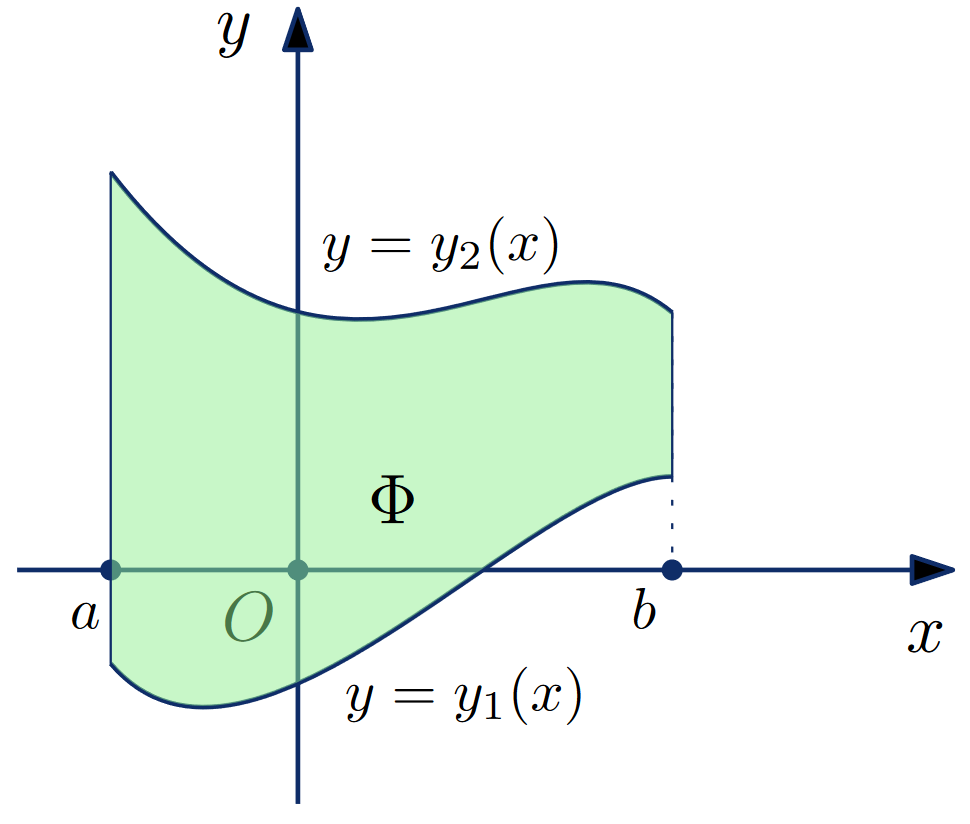
\includegraphics[width=0.4\textwidth]{img/lecture33/the_area_of_the_figure}
    \end{center}
    
    \begin{proof}
    	В предыдущем предложении мы рассматривали неотрицательные функции. Здесь мы можем функции $y_1(x)$ и $y_2(x)$ сдвинуть вверх на одну и ту же константу, таким образом, они станут неотрицательными, если не были таковыми до этого, приэтом искомая площадь останется неизменной.
    	
    	Знаем, что мера Жордана функции $y_2(x)$ - это интеграл $\int_a^b y_2(x) \; dx$, мера Жордана функции $y_1(x)$ - это интеграл $\int_a^b y_1(x) \; dx$. Получается, что мера Жордана искомой площади равна $\int_a^b y_2(x) \; dx - \int_a^b y_1(x) \; dx = \int_a^b (y_2(x) - y_1(x)) \; dx.$
    \end{proof}
    
    \section{Площадь в полярной системе координат}
    
    Полярная система координат — двумерная система координат, в которой каждая точка на плоскости определяется двумя числами — полярным углом и полярным радиусом. 
    \begin{center}
    	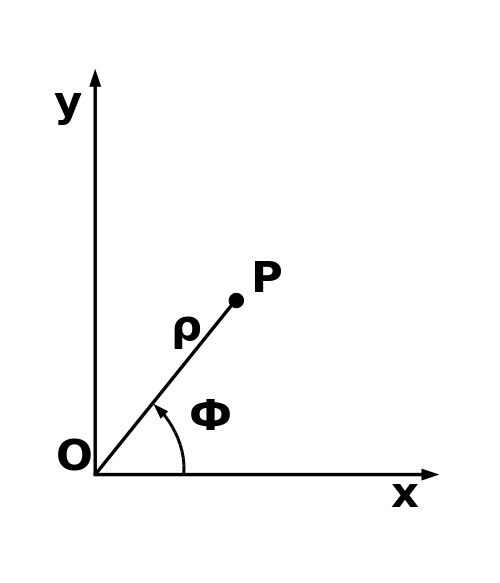
\includegraphics[width=0.3\textwidth]{img/lecture33/polar_coordinates}
    \end{center}
    Пару полярных координат $r$ и $\phi$ можно перевести в Декартовы координаты $x$ и $y$ путём применения тригонометрических функций синуса и косинуса
    \[ x = r\cos{\phi}, y = r\sin{\phi} \]
    Для $r$ = 0, $\phi$ может быть произвольным действительным числом. Для $r \neq 0$, чтобы получить уникальное значение $\phi$, следует ограничиться интервалом $[0, 2\pi)$.
    
    \begin{theorem}
    	Площадь сектора Ф, ограниченного графиком функции $r(\phi)$ в полярных координатах и соответствующими отрезками лучей $\phi = \alpha$ и $\phi = \beta$, равна
    	\[ S = \frac{1}{2} \int_{\alpha}^{\beta} r^2(\phi) \; d\phi. \]
    \end{theorem}
    
    \begin{center}
    	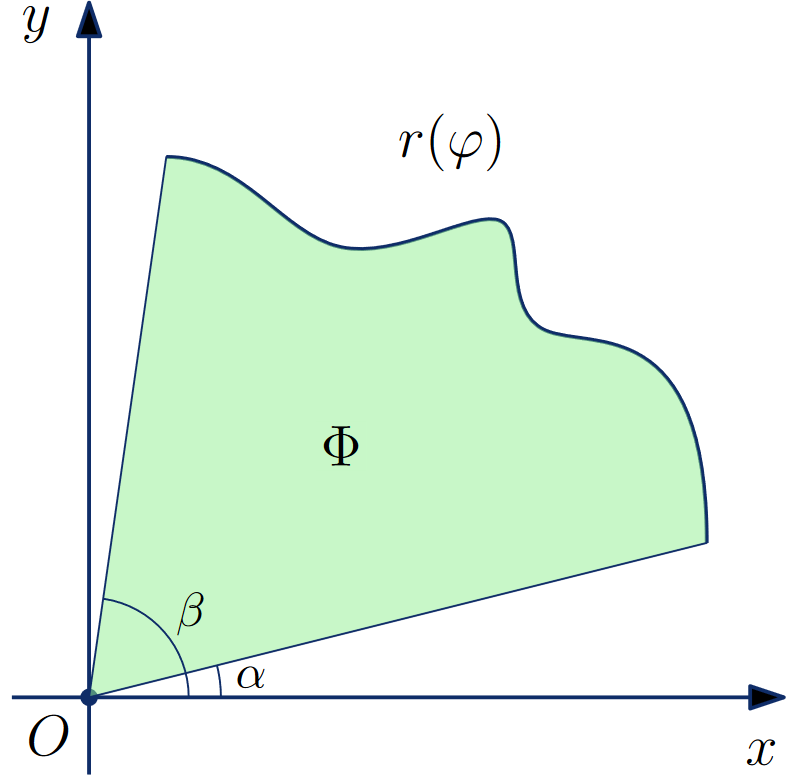
\includegraphics[width=0.3\textwidth]{img/lecture33/the_area_of_the_figure2}
    \end{center}
    
    \begin{proof}
    	Разделим фигуру на секторы, приэтом сначала выберем радиус сектора как минимальное расстояние до начал координат (красные секторы), а затем - как максимальное (зелёные секторы):
   	
   		\begin{center}
   			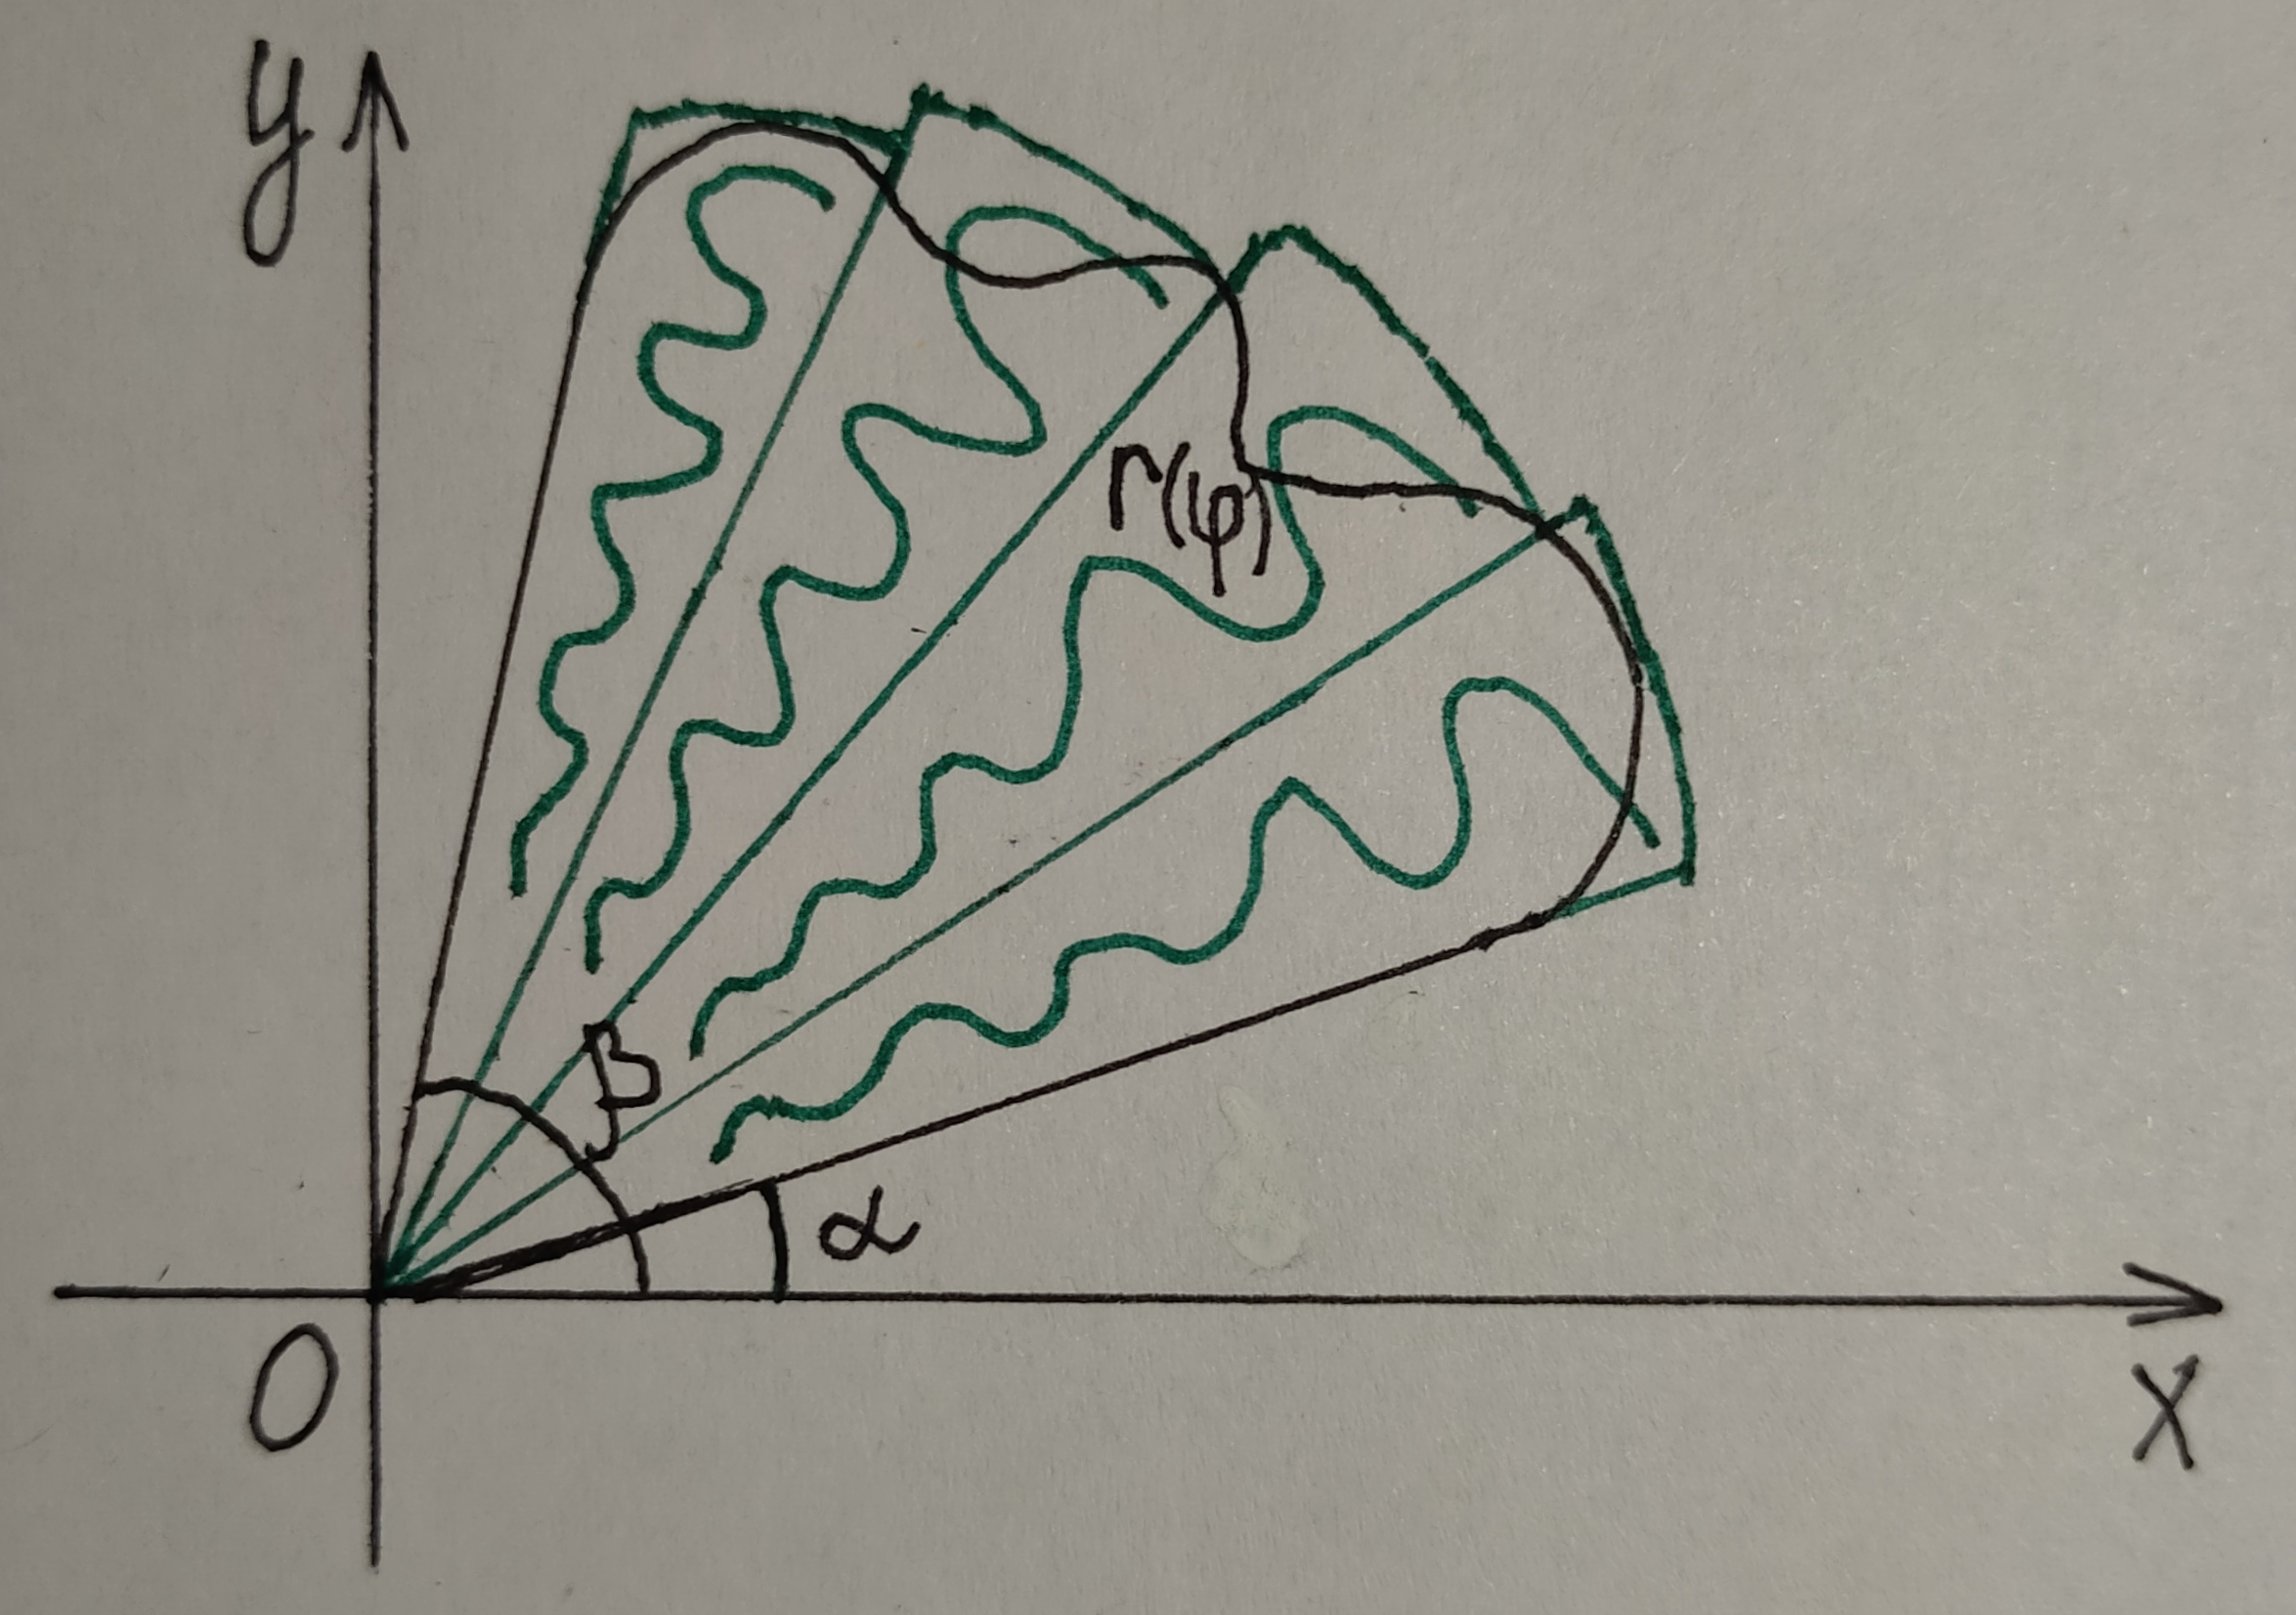
\includegraphics[width=0.3\textwidth]{img/lecture33/max_sectors}
   		\end{center}
   		\begin{center}
   		    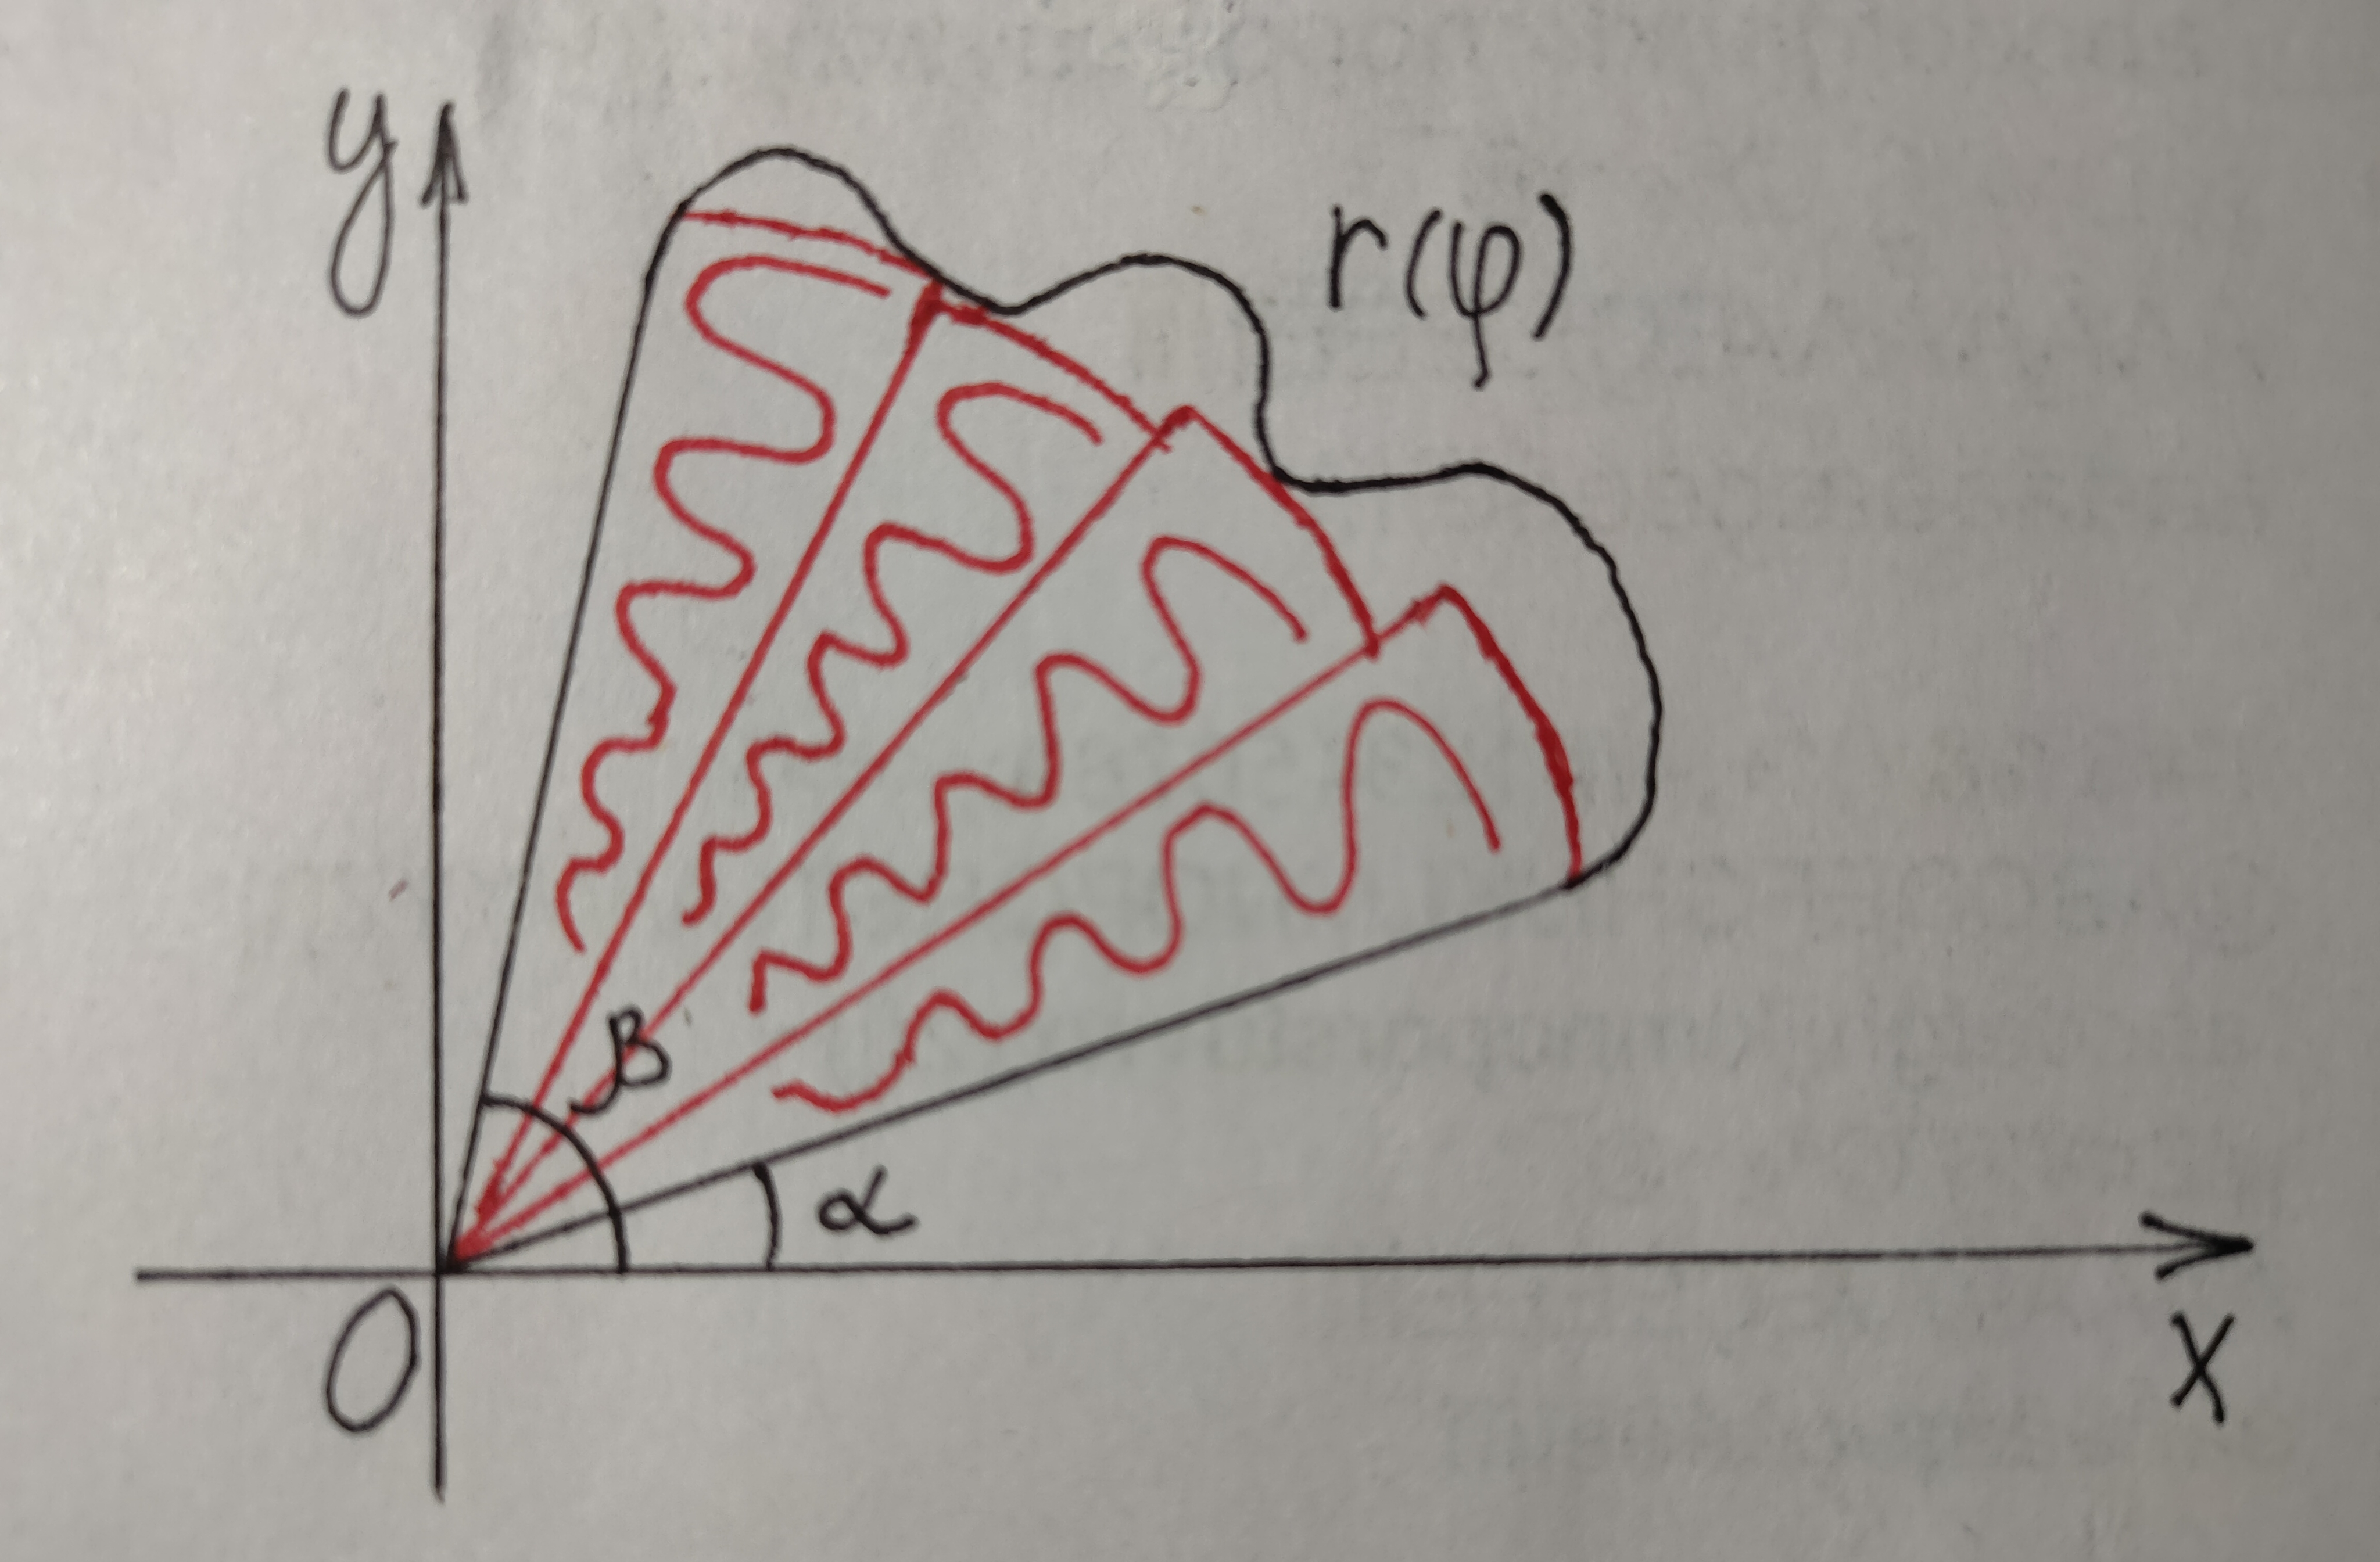
\includegraphics[width=0.3\textwidth]{img/lecture33/min_sectors}
   		\end{center}
   		
   		$T$ - разбиение $[\alpha, \beta]$
   		
   		Формулу площади круга $\pi r^2$ можно доказать, посчитав интеграл $4 \int_0^r \sqrt{r^2 - x^2} \; dx$ (фактически считаем площади четверти круга)
   		
   		\[ 4 \int_0^r \sqrt{r^2 - x^2} \; dx = 4 \int_0^r r\sqrt{1 - (\frac{x}{r})^2} \; dx = [\sin{\phi} = \frac{x}{r} \Rightarrow r\sin{\phi} = x \Rightarrow r\cos{\phi} d\phi = dx] = \] 
   		\[ = 4 \int_0^{\frac{\pi}{2}} r\sqrt{1 - \sin^2{\phi}} \cdot r \cos{\phi} \; d\phi = (*), \]
   		т. к. $\sin{\phi} = \frac{r}{r} = 1 \Rightarrow \phi = \frac{\pi}{2}, \sin{\phi} = \frac{0}{r} = 0 \Rightarrow \phi = 0.$
    	\[ (*) = 4 \int_0^{\frac{\pi}{2}} r \cos{\phi} \cdot r \cos{\phi} d\phi = 4 \int_0^{\frac{\pi}{2}} r^2 \cos^2{\phi} \; d\phi = 4r^2 \int_0^{\frac{\phi}{2}} \cos^2{\phi} \; d\phi = \] 
    	\[ = 4 r^2 \int_0^{\frac{\pi}{2}} \frac{1 + \cos{2\phi}}{2} \; d\phi = 2r^2 \int_0^{\frac{\pi}{2}} (1 + \cos{2\phi}) \; d\phi = 2r^2 \bigg(\phi + \frac{1}{2} \sin{2\phi} \bigg|_0^{\frac{\pi}{2}}\bigg) = \pi r^2 \]
    	
    	Тогда площадь сектора равна
    	\[ S_{(\phi_1, \phi_2)} = \frac{\pi r^2 (\phi_2 - \phi_1)}{2\pi} = \frac{r^2 (\phi_2 - \phi_1)}{2} \]
    	\begin{center}
    		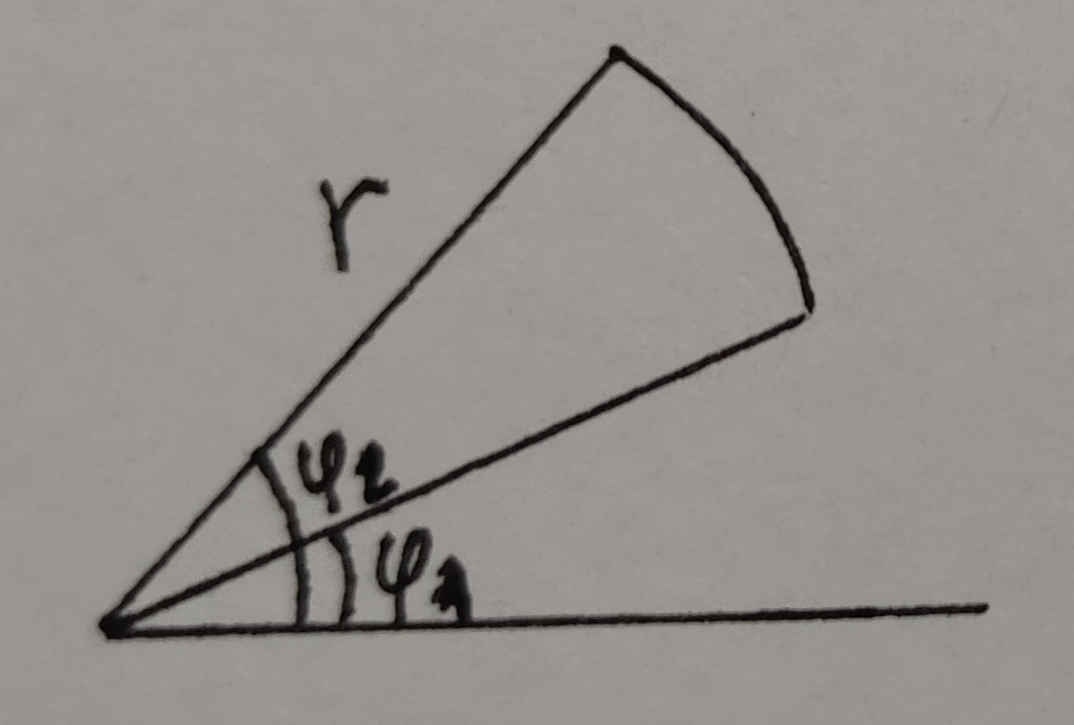
\includegraphics[width=0.2\textwidth]{img/lecture33/sector}
    	\end{center}
    	
    	Площадь красных секторов
    	\[ S_1 = \sum_{k = 1}^n \inf_{\phi \in \Delta_k} r^2(\phi) \frac{1}{2} \Delta\phi_k = s(g, T), \]
    	где $g(r) = \frac{r^2}{2}$, $\Delta\phi_k = \phi_k - \phi_{k - 1}$.
    	
    	Площадь зелёных секторов
    	\[ S_2 = \sum_{k = 1}^n \sup_{\phi \in \Delta_k} r^2(\phi) \frac{1}{2} \Delta\phi_k = S(g, T) \]
    	
    	$S(g, T)$ и $s(g, T)$ стремятся к интегралу. Мера Жордана зажата между ними $\Rightarrow$ тоже стремится к интегралу, т. е. к $\int_{\alpha}^{\beta} \frac{r^2(\phi)}{2} \; d\phi$.
    \end{proof}
    
    \begin{example}
    	На гиперболе $x^2 - y^2 = a^2$ дана точка $M(x_0; y_0)$. Найти площадь криволинейного треугольника OAM. 
    \end{example}
    
    \begin{center}
    	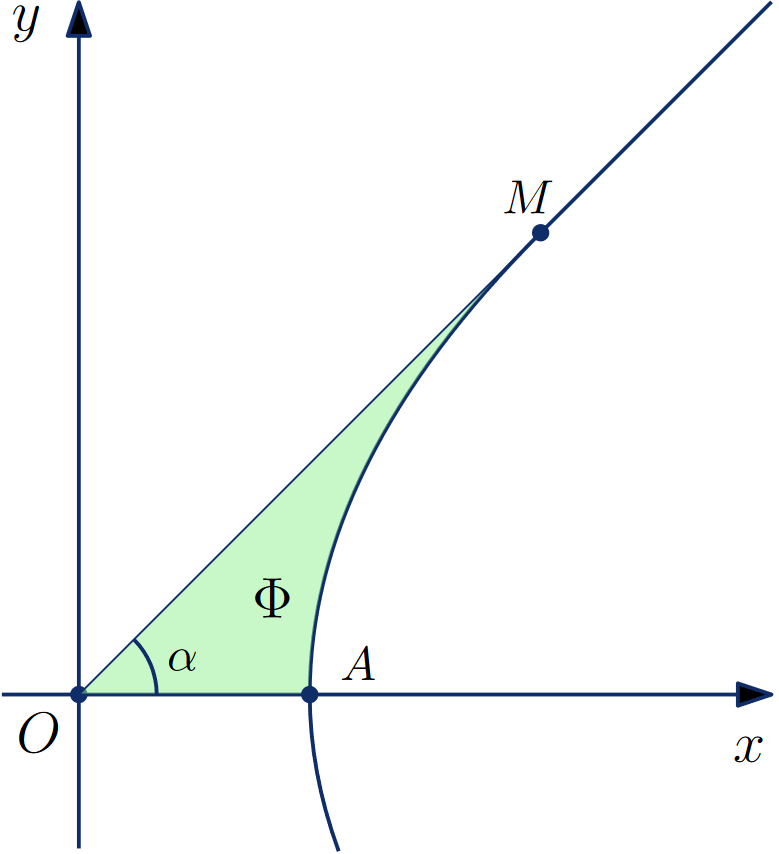
\includegraphics[width=0.3\textwidth]{img/lecture33/the_area_of_the_figure3}
    \end{center}
    
    Зададим в полярной системе координат гиперболу:
    \[ x^2 - y^2 = a^2 \Rightarrow r^2 \cos{\phi}^2 - r^2 \sin^2{\phi} = a^2 \Rightarrow r^2 (\cos{\phi}^2 - \sin{\phi}) = a^2 \Rightarrow r^2 = \frac{a^2}{\cos{2\phi}} \Rightarrow \]
    \[ \Rightarrow r = \frac{a}{\sqrt{\cos{2\phi}}} \]
    
    Угол точки $A$ равен 0, угол точки $M$ равен $\arctg{\frac{y_0}{x_0}}$.
    
    Осталось посчитать интеграл:
    \[ S = \frac{1}{2} \int_0^{\arctg{\frac{y_0}{x_0}}} \frac{a^2}{\cos{2\phi}} \; d\phi = \frac{a^2}{2} \int_0^{\arctg{\frac{y_0}{x_0}}} \frac{\cos{2\phi}}{\cos^2{2\phi}} \; d\phi = \frac{a^2}{4} \int_0^{\arctg{\frac{y_0}{x_0}}} \frac{d\sin{2\phi}}{\cos^2{2\phi}} = \]
    \[ = \frac{a^2}{4} \int_0^{\arctg{\frac{y_0}{x_0}}} \frac{d\sin{2\phi}}{1 - \sin^2{2\phi}} = \frac{a^2}{8} \ln{\bigg|\frac{1 - \sin{2\arctg{\frac{y_0}{x_0}}}}{1 + \sin{2\arctg{\frac{y_0}{x_0}}}}\bigg|} + C = (*) \]
    В силу формулы $\sin{\alpha} = \frac{2\tg{\frac{\alpha}{2}}}{1 + \tg^2{\frac{\alpha}{2}}}$ получаем, что
    \[ (*) = \frac{a^2}{8} \ln{\bigg|\frac{1 - \frac{2 \frac{y_0}{x_0}}{1 + \frac{y_0^2}{x_0^2}}}{1 + \frac{2 \frac{y_0}{x_0}}{1 + \frac{y_0^2}{x_0^2}}}\bigg|} + C \]
    
    \section*{Лекция 34: Метрические, нормированные и евклидовы  пространства}
    
    \section{Объем тел вращения}
    
    \begin{theorem}
    	Пусть функция $y = y(x)$ непрерывна и неотрицательна на отрезке $[a; b]$. Объем $V$ тела, образованного вращением вокруг оси Ox фигуры Ф, ограниченной графиком функции $f(x)$, отрезками прямых $x = a$ и $x = b$ и отрезком оси $Ox$, равен
    	\[ V = \pi \int_a^b f^2(x) \; dx. \]
    \end{theorem}
    
    \begin{center}
    	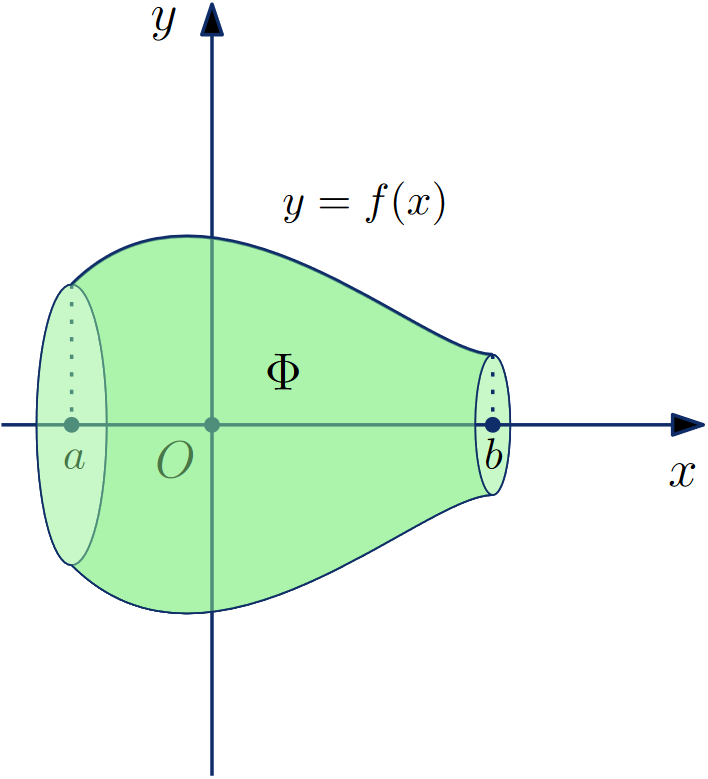
\includegraphics[width=0.3\textwidth]{img/lecture33/the_area_of_the_figure4}
    \end{center}
    
    \begin{proof}
    	Обозначим через $G$ тело, образованное вращением вокруг оси $Ox$ фигуры Ф. Рассмотрим разбиение $T = \{x_0, x_1, ..., x_n\}$ отрезка $[a; b]$. Заметим, что фигура $C_1(T)$, состоящая из цилиндров высоты $h_k = x_k - x_{k - 1}$ радиуса $R = \sup_{x \in \Delta_k} f(x)$, покрывает тело вращения $G$. А фигура $C_2(T)$, состоящая из цилиндров высоты $h_k = x_k - x_{k - 1}$ радиуса $R = \inf_{x \in \Delta_k} f(x)$, наоборот, вписана в тело вращения $G$. Как известно, объем цилиндра радиуса $R$ и высоты $h$ равен $\pi R^2 h$. Отсюда получаем, что
    	\[ \mu(C_2(T)) = \sum_{k = 1}^n \pi \inf_{x \in \Delta_k} f^2(x) \Delta x_k \leqslant \sum_{k = 1}^n \pi \sup_{x \in \Delta_k} f^2(x) \Delta x_k = \mu(C_1(T)). \]
    	В правом и левой частях неравенства стоят в точности нижняя и верхняя суммы Дарбу для функции $\pi f^2(x)$. Поскольку функция $f(x)$ непрерывна, она является интегрируемой (следствие 10.14). А значит интегрируем и ее квадрат (следствие 10.7). Тем самым получаем, что
    	\[ \mu(C_1(T)), \mu(C_2(T)) \to I = \pi \int_a^b f^2(x) \; dx \text{ при } \Delta_T \to 0. \]
    	Это означает, что $G$ измеримо по Жордану, и его объем равен $V = \pi \int_a^b f^2(x) \; dx$.
    \end{proof}
    
    \begin{example}
    	Найти объем тела, образованного при вращении круга $(x - a)^2 + y^2 \leqslant a^2$ вокруг оси Oy.
    \end{example}
    
    \begin{explanation}
    	Хоть здесь фигура вращается вокруг оси $OY$, но нам это не помешает. $(x - a)^2 + y^2 \leqslant a^2$ задаёт круг с центром в точке $(0, a)$ и радиусом $a$. При повороте этой красной окружности получим "бублик". Чтобы посчитать его объём, нужно вычислить объём фигуры, получающейся при вращении вокруг $OY$ правой полуокружности $x(y) = a + \sqrt{a^2 - y^2}$, и вычесть объём фигуры, получающийся при вращении вокруг $OY$ левой полуокружности $x(y) = a - \sqrt{a^2 - y^2}$ (отверстие "бублика"). Пользуясь теоремой 12.5 найдём итоговый объём.
    	\begin{center}
    		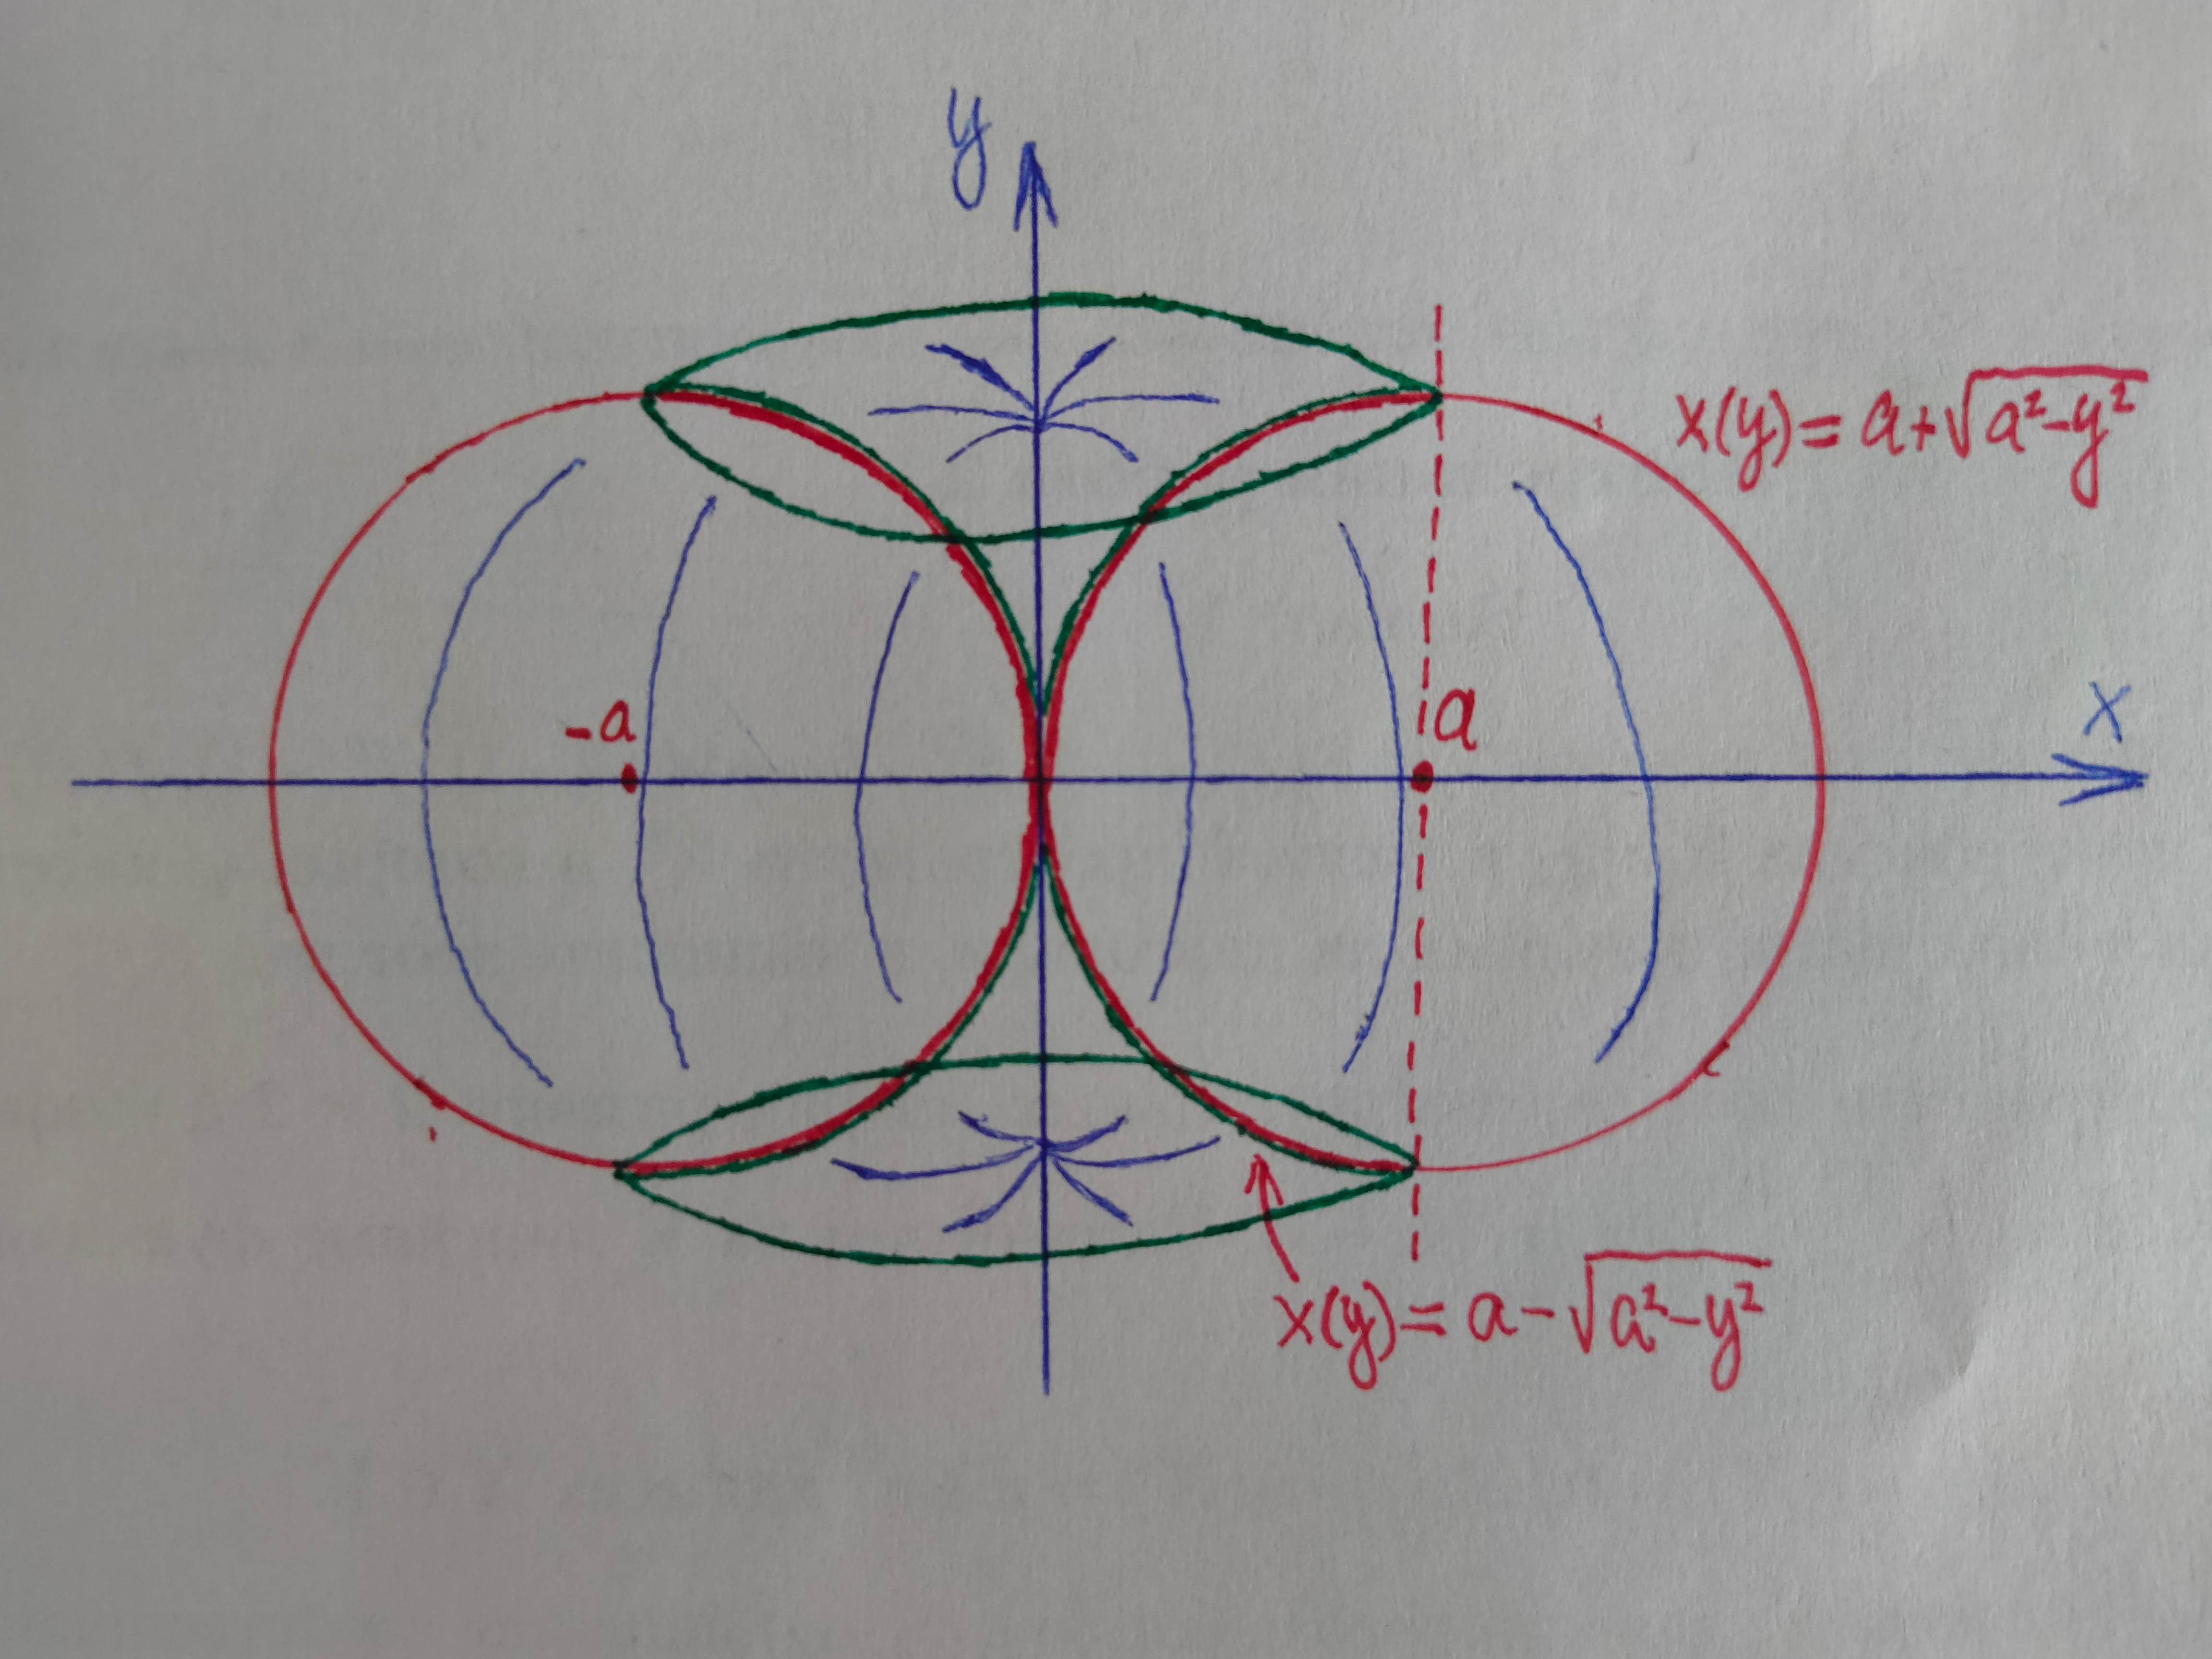
\includegraphics[width=0.5\textwidth]{img/lecture34/plot}
    	\end{center}
    	\[ V = \pi \int_{-a}^a (a + \sqrt{a^2 - y^2})^2 - (a - \sqrt{a^2 - y^2})^2 \; dy = 4\pi \int_{-a}^a a\sqrt{a^2 - y^2} \; dy = \]
    	\[ = 4\pi a \int_{-a}^a \sqrt{a^2 - y^2} \; dy \]
    	Отдельно считаем такой интеграл
    	\[ \int_{-a}^a \sqrt{a^2 - y^2} \; dy = a^2 \int_{-a}^a \sqrt{1 - (\frac{y}{a})^2} \; d(\frac{y}{a}) = a^2 \int_{-1}^1 \sqrt{1 - t^2} \; dt = \]
    	\[ = a^2 \int_{-\frac{\pi}{2}}^{\frac{\pi}{2}} \sqrt{1 - \sin^2{x}} \; d(\sin{x}) = a^2 \int_{-\frac{\pi}{2}}^{\frac{\pi}{2}} \cos{x} \; d(\sin{x}) \]
    	Далее
    	\[ I = \int_{-\frac{\pi}{2}}^{\frac{\pi}{2}} \cos{x} \; d(\sin{x}) = \cos{x} \sin{x} \bigg|_{-\frac{\pi}{2}}^{\frac{\pi}{2}} -  \int_{-\frac{\pi}{2}}^{\frac{\pi}{2}} \sin{x} \; d(\cos{x}) = \int_{-\frac{\pi}{2}}^{\frac{\pi}{2}} \sin^2{x} \; dx = \]
    	\[ = \pi - \int_{-\frac{\pi}{2}}^{\frac{\pi}{2}} \cos^2{x} \; dx = \pi - I \]
    	Тогда
    	\[ \int_{-a}^a \sqrt{a^2 - y^2} \; dy = \frac{a^2 \pi}{2} \]
    	Следовательно
    	\[ V = 4\pi a \int_{-a}^a \sqrt{a^2 - y^2} \; dy = 2a^3 \pi^2 \]
    \end{explanation}
    
    \section{Длина кривой}
    
    Для описания длины дуги кривой мы будем использовать иной подход — определим длину кривой через свойства, которым она должна удовлетворять.
    
    Чтобы этот подход был более понятен, сначала реализуем его на площади фигуры.
    
    Пусть $f \geqslant 0$ на $[a, b]$. И пусть $S(\alpha, \beta)$ площадь под графиком функции $f$ на отрезке $[\alpha, \beta] \subset [a, b]$. Разумные требования на $S$ — это
    \begin{enumerate}
    	\item аддитивность: $S(\alpha, \gamma) = S(\alpha, \beta) + S(\beta, \gamma)$ при $a \leqslant \alpha < \beta < \gamma \leqslant b$;
    	\item монотонность по включению: $\displaystyle \inf_{x \in [\alpha, \beta]} f(x) (\beta - \alpha) \leqslant S(\alpha, \beta) \leqslant \sup_{x \in [\alpha, \beta]} f(x) (\beta - \alpha).$
    \end{enumerate}
    
    \begin{sentence}
    	Пусть $f$ интегрируема по Риману на $[a, b]$. При выполнении выше описанных условий $S(a, b) = \int_a^b f(x) \; dx$.
    \end{sentence}
    
    \begin{proof}
    	$T = \{x_0, x_1, ..., x_n\}$ - разбиение $[a, b]$, $I = \int_a^b f(x) \; dx$.
    	\[ \sum_{k = 1}^n \inf_{x \in \Delta_k} f(x) \Delta x_k \leqslant (\text{аддитивность}) \sum_{k = 1}^n S(x_{k - 1}, x_k) = (\text{монотонность по включению}) \]
    	\[ = S(a, b) \leqslant \sum_{k = 1}^n \sup_{x \in \Delta_k} f(x) \Delta x_k (\text{аналогично}) \]
    	Если функция интегрируема, то
    	\[ \sum_{k = 1}^n \inf_{x \in \Delta_k} f(x) \Delta x_k \to I, \sum_{k = 1}^n \sup_{x \in \Delta_k} f(x) \Delta x_k \to I \Rightarrow S(a, b) \to I \Rightarrow S(a, b) = I \]
    	(т. к. площадь константа).
    \end{proof}
    
    \begin{definition}
    	Пусть $\gamma : [a, b] \rightarrow \R^3$ - гладкая кривая, т.е. $\gamma(t) = (x(t), y(t), z(t))$ и функции $x, y, z \in C^1([a, b])$ (множество функций, у которых первая производная непрерывна). Пусть $\ell(a, b)$ — длина пути соответствующая отрезку $[a, b]$. Тогда длина кривой удовлетворяет следующим требованиям
        \begin{enumerate}
        	\item $\ell(\alpha, \gamma) = \ell(\alpha, \beta) + \ell(\beta, \gamma)$ при $a \leqslant \alpha < \beta < \gamma \leqslant b$;
        	\item $\displaystyle\inf_{t \in [\alpha, \beta]} |v(t)|(\beta - \alpha) < \ell(\alpha, \beta) \leqslant \sup_{t \in [\alpha, \beta]} |v(t)|(\beta - \alpha)$, где $v(t) = (x'(t), y'(t), z'(t))$.
        \end{enumerate}
    \end{definition}
    
    \begin{theorem}
    	Длина кривой, заданной параметрически уравнениями
    	\[ x = x(t), y = y(t), z = z(t), t \in [a; b], \]
    	где $x(t), y(t), z(t)$ - непрерывно дифференцируемые на $[a; b]$ функции, равна
    	\[ s = \int_a^b \sqrt{(x'(t))^2 + (y'(t))^2 + (z'(t))^2} \; dx \]
    \end{theorem}
    
    \begin{proof}
    	Задаём прямую в $\R^3$, введя при этом параметр $t \in \R$ и точки $(x(t), y(t), z(t))$. Во втором пункте $v(t), t \in [\alpha, \beta]$ - это скорость движения по кривой на временном отрезке $[\alpha, \beta]$. Тогда $|v(t)|(\beta - \alpha)$ - это длина кривой на отрезке $[\alpha, \beta]$. Используя физическую интерпретацию, утверждаем, что скорость - производная по каждой координате: $v = (x'(t), y'(t), z'(t))$. Значит $|v(t)| = \sqrt{(x'(t))^2 + (y'(t))^2 + (z'(t))^2}$.
    	
        Рассмотрим разбиение времени $T = \{t_0, t_1, ..., t_n\}$, $\Delta t_k$ - длина отрезка разбиения. По определению
        \[ \inf_{t \in \Delta_k} |v(t)| \cdot \Delta t_k \leqslant \ell(\Delta t_k) \leqslant \sup_{t \in \Delta_k} |v(t)| \cdot \Delta t_k \]
        По первому свойству
        \[ \sum_{k = 1}^n \inf_{t \in \Delta_k} |v(t)| \cdot \Delta t_k \leqslant \ell(a, b) \leqslant \sum_{k = 1}^n \sup_{t \in \Delta_k} |v(t)| \cdot \Delta t_k \]
        $x(t), y(t), z(t)$ - непрерывно дифференцируемые на $[a; b]$ функции $\Rightarrow$ функция $|v(t)| = \sqrt{(x'(t))^2 + (y'(t))^2 + (z'(t))^2}$ - непрерывна. Значит она интегрируема.
        
        Выше мы записали интегральные суммы Дарбу для этой функции $\Rightarrow$
        \[ \sum_{k = 1}^n \inf_{t \in \Delta_k} |v(t)| \cdot \Delta t_k \to I, \sum_{k = 1}^n \sup_{t \in \Delta_k} |v(t)| \cdot \Delta t_k \to I, I = \int_a^b |v(t)| \; dt. \]
    \end{proof}
    
    \chapter{Предел функции нескольких переменных}
    
    \section{Метрическое пространство}
    
    \begin{definition}
    	Пусть $X$ - множество. Функция $d: X \times X \rightarrow [0, +\infty)$ называется \underline{метрикой}, если
    	\begin{enumerate}
    		\item $d(x, y) = 0 \Leftrightarrow x = y;$
    		\item $d(x, y) = d(y, x)$ $\forall x, y \in X;$
    		\item $d(x, z) \leqslant d(x, y) + d(y, z)$ $\forall x, y, z \in X.$
    	\end{enumerate}
    	Пара $(X, d)$ называется \underline{метрическим пространством}.
    \end{definition}
    
    \begin{example}
    	\begin{itemize}
    		\item \underline{Дискретная метрика}: $d(x, y) = 0$, если $x = y$, и $d(x, y) = 1$ во всех остальных случаях.
    		\item \underline{Вещественные числа} с функцией расстояния $d(x, y) = |y - x|$ и евклидово пространство являются полными метрическими пространствами.
    		\item \underline{Расстояние Хэмминга} в теории кодирования.
    		
    		(Расстояние Хэмминга - функция расстояния между двоичными словами, которая равна количеству битов, в которых эти слова различаются. Другими словами - это минимальная длина пути от одного двоичного слова до другого в булевом кубе)
    		\item \underline{Манхэттенская метрика}: $d(\textbf{p}, \textbf{q}) = \sum^n_{i = 1} |p_i - q_i|$,
    		где $\textbf{p} = (p_1, p_2, ..., p_n), \textbf{q} = (q_1, q_2, ..., q_n)$ — векторы.
    	\end{itemize}
    \end{example}
    
    \section{Нормированное пространство}
    
    \begin{definition}
    	Пусть $X$ — линейное пространство. Функция
    	$||\cdot||: X \rightarrow [0, +\infty)$ называется \underline{нормой}, если
    	\begin{enumerate}
    		\item $||x|| = 0 \Leftrightarrow x = 0;$
    		\item $||\lambda x|| = |\lambda| ||x||$ $\forall x \in X;$
    		\item $||x + y|| \leqslant ||x|| + ||y||$ $\forall x, y \in X.$
    	\end{enumerate}
    	Пара $(X, ||\cdot||)$ называется \underline{нормированным пространством}.
    \end{definition}
    Всякое нормированное пространство является метрическим с метрикой $d(x, y) = ||x - y||$.
    
    Проверяем свойства метрического пространства.
    \begin{enumerate}
    	\item $d(x, y) = 0 \Leftrightarrow ||x - y|| = 0 \Leftrightarrow x - y = 0 \Leftrightarrow x = y.$
    	\item $d(x, y) = ||x - y|| = |-1|||y - x|| = ||y - x||$
    	\item $d(x, z) \leqslant d(x, y) + d(y, z) \Leftrightarrow ||x - z|| \leqslant ||x - y|| + ||y - z|| \Leftrightarrow  ||a + b|| \leqslant ||a|| + ||b||$, где $a = x - y, b = y - z$.
    \end{enumerate}
    
    \section{Евклидово пространство}
    
    \begin{definition}
    	Пусть $X$ — линейное пространство. Функция $\langle\cdot, \cdot\rangle: X \times X \rightarrow \R$ называется скалярным произведением, если для всех $x, y, z \in X$ и всех $a, b \in \R$ выполнены следующие условия:
    	\begin{enumerate}
    		\item $\langle x, x \rangle \geqslant 0$ и $\langle x, x \rangle = 0 \Leftrightarrow x = 0;$
    		\item $\langle x, y \rangle = \langle y, x \rangle;$
    		\item $\langle ax + by, z \rangle = a\langle x, z \rangle + b\langle y, z \rangle.$
    	\end{enumerate}
    	Линейное пространство $X$ со скалярным произведением называется \underline{евклидовым}.
    \end{definition}
    
    \begin{example}
    	На линейном пространстве $\R^k$ всех упорядоченных наборов $(x_1, ..., x_k)$ задано скалярное произведение $\langle x, y \rangle := \sum_{j = 1}^k x_j y_j.$ Тем самым, на $\R^k$ задана естественная евклидова метрика
    	\[ ||x - y|| := \sqrt{|x_1 - y_1|^2 + ... + |x_k - y_k|^2}. \]
    \end{example}
    
    \section{Неравенство Коши–Буняковского}
    
    \begin{lemma}[Неравенство Коши–Буняковского]
    	Пусть $\langle \cdot, \cdot \rangle$ скалярное произведение на линейном пространстве $X$, тогда
    	\[ |\langle x, y \rangle| \leqslant \sqrt{\langle x, x \rangle} \sqrt{\langle y, y \rangle}. \]
    \end{lemma}
    
    \begin{proof}
    	Рассмотрим скалярный квадрат: $\langle x + yt, x + yt \rangle \geqslant 0, t \in \R, x, y \in X$. Воспользуемся линейностью
    	\[ 0 \leqslant \langle x + yt, x + yt \rangle = \langle x, x \rangle + \langle x, yt \rangle + \langle yt, x \rangle + \langle yt, yt \rangle = \langle x, x \rangle + 2t\langle x, y \rangle + t^2\langle y, y \rangle \]
        Если $\vec{y} = 0$, то просто подставим в исходное неравенство и получим $0 \leqslant 0$. Теперь пусть $\vec{y} \neq 0$. Чтобы неравенство $\langle x, x \rangle + 2t\langle x, y \rangle + t^2\langle y, y \rangle \geqslant 0$ выполнялось, необходимо, чтобы $D = 4\langle x, y \rangle^2 - 4 \langle y, y \rangle \langle x, x \rangle \leqslant 0$. Тогда
        \[ \langle x, y \rangle^2 \leqslant \langle y, y \rangle \langle x, x \rangle \]
    \end{proof}
    
    \begin{corollary}
    	На евклидовом пространстве функция $||x|| := \sqrt{\langle x, x \rangle}$ является нормой.
    \end{corollary}
    
    \begin{enumerate}
    	\item По свойству скалярного произведения $||x|| = \langle x, x \rangle = 0 \Leftrightarrow x = 0$.
    	\item $||\lambda x|| = \sqrt{\langle \lambda x, \lambda x \rangle} = |\lambda| \sqrt{\langle x, x \rangle} = |\lambda| ||x||$
    	\item $||x + y||^2 = \langle x + y, x + y \rangle = \langle x, x \rangle + 2 \langle x, y \rangle + \langle y, y \rangle \leqslant \text{(нер-во Коши-Буняковского)}$ $\langle x, x \rangle + 2\sqrt{\langle x, x \rangle} \sqrt{\langle y, y \rangle} + \langle y, y \rangle = (\sqrt{\langle x, x \rangle} + \sqrt{\langle y, y \rangle})^2 = (||x|| + ||y||)^2$
    \end{enumerate}
    
    \section{Предел в метрическом пространстве}
    
    \begin{definition}
    	Пусть $(X, d)$ метрическое пространство.
    	\begin{enumerate}
    		\item Множество
    		\[ B_r(x_0) := \{x \in X: d(x, x_0) < r\} \]
    		называется открытым шаром радиуса $r$.
    		\item Последовательность точек $x_n \in X$ называется сходящейся к точке $x$, если для всякого $\epsilon > 0$ найдется такой номер $N(\epsilon)$, что $d(x, x_n) < \epsilon$ для каждого $n \geqslant N(\epsilon)$.
    		\item Точка $x$ называется предельной для множества $M \subset X$, если для всякого $\epsilon > 0$ выполнено $B_{\epsilon}(x) \cap (M \setminus \{x\}) \neq \varnothing.$
    		\item Точка x называется изолированной для множества $M \subset X$, если $\exists \epsilon > 0$, такое что 	$B_{\epsilon}(x) \cap (M \setminus \{x\}) = \varnothing$.
    	\end{enumerate}
    \end{definition}
    
    \begin{lemma}
    	Пусть $(X, d)$ метрическое пространство. Тогда
    	\begin{enumerate}
    		\item если $x_n \rightarrow x, y_n \rightarrow y$, то $d(x_n, y_n) \rightarrow d(x, y);$
    		\item предел сходящейся последовательности единственен.
    	\end{enumerate}
    \end{lemma}
    
    \begin{proof}
    	\begin{enumerate}
    		\item Пусть $x_n \to x, y_n \to y$
    		\[ |d(x_n, y_n) - d(x, y)| = |d(x_n, y_n) - d(x_n, y) + d(x_n, y) - d(x, y)| \leqslant |d(x_n, y_n) - d(x_n, y)| + \]
    		\[ + |d(x_n, y) - d(x, y)| \text{ } (*) \]
    		\[ d(x_n, y_n) \leqslant d(x_n, y) + d(y_n, y) \Rightarrow d(x_n, y_n) - d(x_n, y) \leqslant d(y_n, y) \]
    		\[ d(x_n, y) \leqslant d(x_n, x) + d(x, y) \Rightarrow d(x_n, y) - d(x, y) \leqslant d(x_n, x) \]
    		\[ (*): |d(x_n, y_n) - d(x_n, y)| + |d(x_n, y) - d(x, y)| \leqslant d(y_n, y) + d(x_n, x) \]
    		Т. к. $d(y_n, y) \to 0, d(x_n, x) \to 0$, то $d(y_n, y) + d(x_n, x) \to 0 \Rightarrow d(x_n, y_n) \to d(x, y)$.
    		\item Пусть $x_n \to x, x_n \to y$. По первому пункту $d(x_n, x_n) \to d(x, y)$. Т. к. $d(x_n, x_n) = 0$, то $d(x, y) = 0 \Rightarrow x = y$ (по определению).
    	\end{enumerate}
    \end{proof}
    
    \newpage
    
    \section*{Лекция 35: Предел и непрерывность функции нескольких переменных}
    
    Из второго пункта определения 13.8 получаем, что для $x_n \in \R^n$
    \[ x_n \to x \Leftrightarrow \forall \epsilon > 0 \text{ } \exists N: \forall n \geqslant N \rightarrow ||x_n - x|| < \epsilon \] 
    
    \section{Метрическое пространство}
    
    \begin{mention}
    	На $\R^k$ справедливы соотношения
    	\[ \max_{1 \leqslant j \leqslant k} |x_j| \leqslant ||x|| \leqslant \sqrt{k} \max_{1 \leqslant j \leqslant k} |x_j| \]
    	для векторов $x = (x_1, ..., x_k)$. Тем самым, последовательность $x_n \rightarrow x$ в $\R^k$ тогда и только тогда, когда $(x_n)_j \rightarrow x_j$.
    \end{mention}
    
    \begin{explanation}
    	$x = (x_1, ..., x_n) \in \R^n, ||x|| = \sqrt{x_1^2 + x_2^2 + ... + x_n^2}$ (рассматриваем евклидово пространство, см. пример 13.5)
    	\[ \max_{1 \leqslant j \leqslant n} |x_j| = \sqrt{0 + ... + 0 + \max_{1 \leqslant j \leqslant n} x_j^2 + 0 + ... + 0} \leqslant \sqrt{x_1^2 + x_2^2 + ... + x_n^2} \leqslant \sqrt{n} \max_{1 \leqslant j \leqslant n} |x_j| \]
    	Получили неравенство выше.
    
    	Пусть $x_n \to x (\Leftrightarrow x_n - x \to 0) \Leftrightarrow ||x_n - x|| \to 0$. Поэтому будем рассматривать пределы векторов, которые стремятся к нулевому вектору.
    	\begin{enumerate}
    		\item $\forall j$ $x_j \to 0 \Rightarrow x \to 0$, т. к. $||x|| \leqslant \sqrt{n} \max_{1 \leqslant j \leqslant k} |x_j|$.
    		\item $\forall j$ $x \to 0 \Rightarrow ||x|| = 0 \Rightarrow x_j \to 0$, т. к. $\max_{1 \leqslant j \leqslant k} |x_j| \leqslant ||x||$.
    	\end{enumerate}
    \end{explanation}
    
    \begin{sentence}
    	Пусть $x_n \rightarrow x, y_n \rightarrow y$ в нормированном пространстве $(X, ||\cdot||)$ и $\alpha_n \rightarrow \alpha_0$ в $\R$. Тогда $x_n + y_n \rightarrow x + y$ и $\alpha_n x_n \rightarrow \alpha_0 x$ в $X$.
    \end{sentence}
    
    \begin{proof}
    	$||x_n + y_n - (x + y)|| \leqslant ||x_n - x|| + ||y_n - y|| \to 0 + 0 = 0$
    	
    	$||\alpha_n x_n - \alpha_0 x|| = ||\alpha_n x_n - \alpha_n x + \alpha_n x - \alpha_0 x|| \leqslant ||\alpha_n x_n - \alpha_n x|| + ||\alpha_n x - \alpha_0 x|| = |\alpha_n| \cdot ||x_n - x|| + |\alpha_n - \alpha_0| \cdot ||x|| \to |\alpha_0| \cdot 0 + 0 \cdot ||x|| = 0$
    \end{proof}
    
    
    \section{Предел функции по Гейне}
    
    \begin{definition}[предела функции по Гейне]
    	Пусть $(X, d_X)$ и $(Y, d_Y)$ два метрических пространства, $a$ - предельная точка множества $X$. Пусть $f : X \setminus \{a\} \rightarrow Y$. Говорят, что $A \in Y$ предел функции $f$ при $x \rightarrow a$, если для каждой  последовательности $x_n \in X \setminus \{a\}, x_n \rightarrow a$, выполнено $f(x_n) \rightarrow A$. Пишут $\displaystyle \lim_{x \rightarrow a} f(x) = A$ или $f(x) \rightarrow A$ при $x \rightarrow a$.
    \end{definition}
    
    \begin{sentence}
    	Если $\displaystyle \lim_{x \rightarrow a} f(x) = A$ и $\displaystyle \lim_{x \rightarrow a} f(x) = B$, то $A = B$.
    \end{sentence}
    
    \begin{proof}
    	$a$ - предельная точка $\Rightarrow \exists x_n \in X \backslash \{a\} : x_n \to a \Rightarrow f(x_n) \to A, f(x_n) \to B$ по определению предела функции по Гейне. Но $y_n = f(x_n)$ - последовательность векторов. А мы уже выяснили, что если у последовательности векторов есть предел, то он один (лемма 13.9).
    \end{proof}
    
    \section{Предел функции по Коши}
    
    \begin{definition}[предела функции по Коши]
    	Пусть $(X, d_X)$ и $(Y, d_Y)$ два метрических пространства, $a$ —
    	предельная точка множества $X$. Пусть $f : X \setminus \{a\} \rightarrow Y$. Говорят, что $A \in Y$ предел функции $f$ при $x \rightarrow a$, если для каждого $\epsilon > 0$ найдется такое $\delta > 0$, что $d_Y(f(x), A) < \epsilon$ для каждого такого $x \in X$, что $0 < d_X(x, a) < \delta$.
    \end{definition}
    
    \section{Эквивалентность определений предела}
    
    \begin{theorem}
    	Определения по Коши и по Гейне равносильны.
    \end{theorem}
    
     \begin{proof}
    	$ $
    	
    	\begin{itemize}
    		\item[$\text{K} \Rightarrow \text{Г}$] Пусть $A = \lim_{x \to a} f(x)$ по Коши.
    		\[ \forall \epsilon > 0 \text{ } \exists \delta > 0: \forall x \in B'_{\delta}(a) \rightarrow ||f(x) - A|| < \epsilon \]
    		Пусть $x_n \in X \backslash \{a\}, x_n \to a \Rightarrow \exists N: \forall n \geqslant N \rightarrow ||x_n - a|| < \delta \Leftrightarrow x_n \in B'_{\delta}(a) \Rightarrow \forall n \geqslant N \rightarrow ||f(x_n) - A|| < \epsilon \Rightarrow f(x_n) \rightarrow A$
    		\item[$\text{Г} \Rightarrow \text{К}$] $\Leftrightarrow \neg \text{К} \Rightarrow \neg \text{Г}$
    		\[ \neg\text{К} \Rightarrow \exists \epsilon > 0 : \forall \delta > 0 \text{ } \exists x \in B'_{\delta}(a) : ||f(x) - A|| \geqslant \epsilon \]
    		Для каждого $\delta = \frac{1}{n}$ $\exists x_n \in B'_{\frac{1}{n}}(a) : ||f(x_n) - A|| \geqslant \epsilon$
    		
    		Но $x_n \in X \backslash \{a\}, x_n \to a$ и $f(x_n) \not\to A \Rightarrow \neg \text{Г}$.         
    	\end{itemize}
    \end{proof}
    
    \section{Арифметические свойства предела}
    
    \begin{theorem}[Арифметические свойства предела]
    	Пусть $(X, d_X)$ метрическое пространство, $a$ — предельная
    	точка $X$. Пусть $f, g : X \setminus \{a\} \rightarrow \R^k,  \alpha : X \setminus \{a\} \rightarrow \R$. Если $\displaystyle \lim_{x \to a} f(x) = A, \lim_{x \to a} g(x) = B, \lim_{x \to a} \alpha(x) = \alpha_0$, то $\displaystyle \lim_{x \to a} (f(x) + g(x)) = A + B, \lim_{x \to a} (\alpha(x)f(x)) = \alpha_0 A.$
    \end{theorem}
    
    \begin{proof}
    	По определению предела функции по Гейне, если $a$ - предельная точка, то $\forall x_n \in X \backslash \{a\}, x_n \to a$ выполнено $f(x_n) \to A, g(x_n) \to B \Rightarrow f(x_n) + g(x_n) \to A + B$, т. к. $f(x_n), g(x_n)$ - векторы (см. предложение 13.11).
    	
    	По определению предела функции по Гейне, если $a$ - предельная точка, то $\forall x_n \in X \backslash \{a\}, x_n \to a$ выполнено $f(x_n) \to A, \alpha(x_n) \to \alpha_0 \Rightarrow \alpha(x_n) f(x_n) \to \alpha_0 A$, т. к. $f(x_n)$ - вектор (см. предложение 13.11).
    \end{proof}
    
    \section{Теорема о пределе сложной функции}
    
    \begin{theorem}[О пределе сложной функции]
    	Пусть $X, Y, Z$ — метрические пространства, $a$ — предельная точка $X, b$ — предельная точка $Y$. Пусть $f : X \setminus \{a\} \rightarrow Y \setminus \{b\}$ и $g : Y \setminus \{b\} \rightarrow Z$. Если $\displaystyle \lim_{x \to a} f(x) = b$ и $\displaystyle \lim_{y \to b} g(y) = c$, то $\displaystyle \lim_{x \to a} g(f(x)) = c$.
    \end{theorem}
    
    \begin{proof}
    	$ $
    	\begin{center}
    		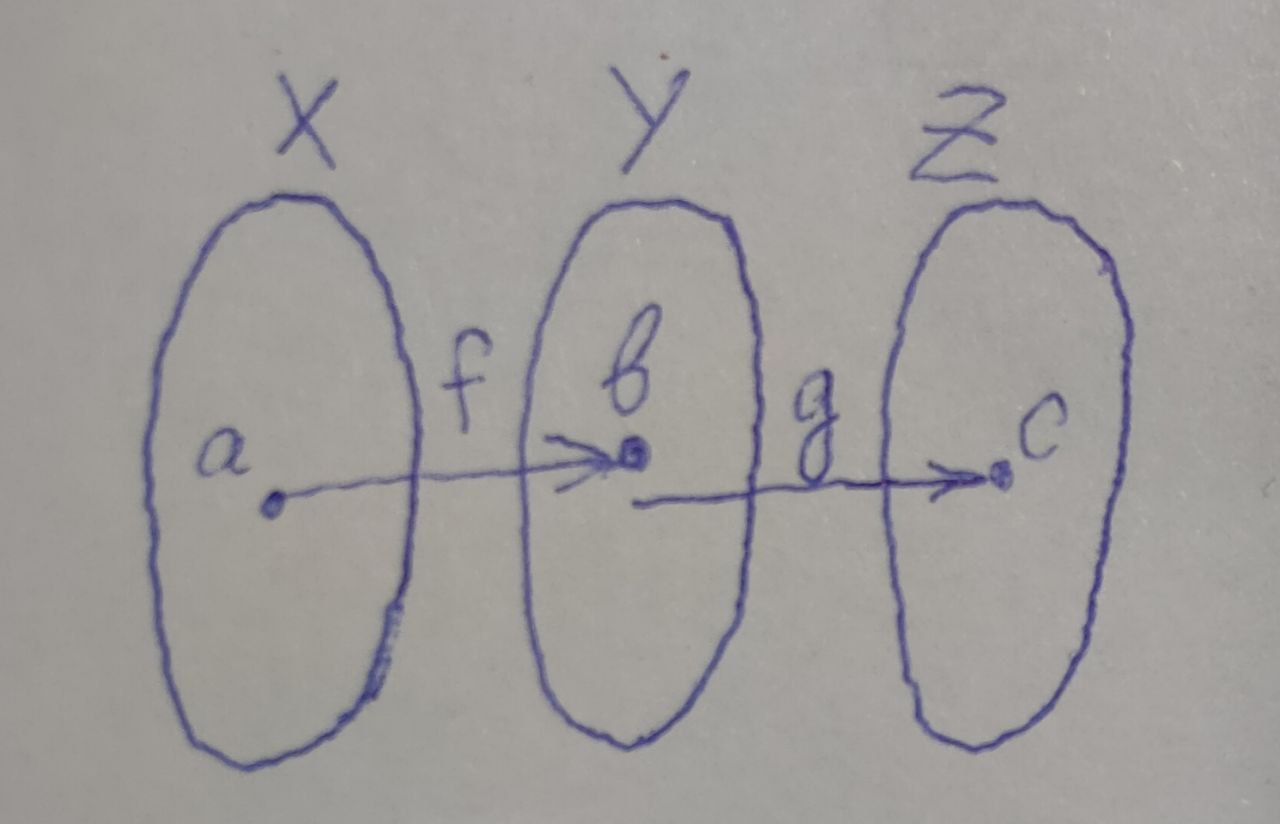
\includegraphics[width=0.3\textwidth]{img/lecture35/limit_of_a_complex_function}
    	\end{center}
    	По определению предела функции по Гейне если $a$ - предельная точка, то $\forall x_n \in X \backslash \{a\}, x_n \to a$ выполнено $f(x_n) \in Y \backslash \{b\}, f(x_n) \to b \Rightarrow g(f(x_n)) \to c$.
    \end{proof}
    
    Важно: исключение из множеств $X$ и $Y$ точек $a$ и $b$ в функции $f: X \setminus \{a\} \rightarrow Y \setminus \{b\}$ обязательно. Контрпример:
    \begin{equation*}
    	f(x) = 0 \text{ } \forall x, g(y) = 
    	\begin{cases}
    		1, & y \neq 0 \\
    		0, & y = 0
    	\end{cases}
    \end{equation*}
    Тогда $\lim_{x \to 0} f(g(x)) = 0, \lim_{y \to 0} g(y) = 1$.
    
    \section{Непрерывность функции}
    
    \begin{definition}
    	Пусть $(X, d_X)$ и $(Y, d_Y)$ два метрических пространства. Отображение $f : X \rightarrow Y$ называется непрерывным в точке $x_0 \in X$, если $\displaystyle \lim_{x \to x_0} f(x) = f(x_0)$ или $x_0$ — изолированная точка.
    \end{definition}
    
    \begin{mention}
    	\begin{enumerate}
	    	\item Если функция $f(x)$ непрерывна в точке a, то для всякой последовательности $x_n \rightarrow a$ выполнено $f(x_n) \rightarrow f(a)$. Это отличается от определения предела функции по Гейне тем, что не требуется брать $x_n$ отличными от $a$. 
	    	
	    	\item То же верно и для определения предела по Коши в случае непрерывности: для всякого $\epsilon > 0$ найдется $\delta > 0$ такое, что $d_Y(f(x), f(x_0)) < \epsilon$, если $d_X(x, x_0) < \delta$.
    	\end{enumerate}
    \end{mention}
    
    \begin{explanation}
    	\begin{enumerate}
    		\item Если $x_0$ - изолированная точка, то любая последовательность, стремящаяся к $x_0$, состоит только из точек $x_0 \Rightarrow f(x_n) \rightarrow f(x_0)$.
    		
    		Пусть $\forall x_n (\neq x_0) \to x_0$ $f(x_n) \to f(x_0)$. От противного: пусть $\exists x_n \to x_0 : f(x_n) \not\rightarrow f(x_0)$, т. е.
    		\[ \exists \epsilon > 0 \text{ } \forall N: \exists n \geqslant N \rightarrow ||f(x_n) - f(x_0)|| \geqslant \epsilon \Rightarrow \]
    		\[ \Rightarrow x_n \neq x_0 (\text{т. к. } \epsilon > 0) \Rightarrow \exists x_n (\neq x_0) \to x_0 \text{ } ||f(x_n) - f(x_0))|| \geqslant \epsilon - \text{противоречие.} \]
    		\item Если $x_0$ - изолированная, то найдётся такое $\delta$-окрестность, что других точек в ней нет:
    		\[ \forall \epsilon > 0 \text{ } \exists \delta > 0: \forall x \in B_{\delta}(x_0) \rightarrow ||f(x) - f(x_0)|| < \epsilon \]
    		Если $x_0$ - предельная, то $\lim_{x \to x_0} f(x) = f(x_0) \Leftrightarrow \forall \epsilon > 0$ $\exists \delta > 0: \forall x \in B'_{\delta}(x_0) \rightarrow ||f(x) - f(x_0)|| < \epsilon$ - условие верно, т. к. оно строже.
    		
    		В обратную сторону.
    		
    		Если $\forall \epsilon > 0 \text{ } \exists \delta > 0: \forall x \in B_{\delta}(x_0) \rightarrow ||f(x) - f(x_0)|| < \epsilon$ - верно, то изолированная точка $x_0$ подходит.
    		
    		Теперь возьмём ту же $\delta$ что и в условии выше. Тогда для $x \neq x_0$ верно $\lim_{x \to x_0} f(x) = f(x_0) \Leftrightarrow \forall \epsilon > 0$ $\exists \delta > 0: \forall x \in B'_{\delta}(x_0) \rightarrow ||f(x) - f(x_0)|| < \epsilon$, а для $x = x_0$ $||f(x) - f(x_0)|| = 0 < \epsilon$ - тоже верно.
    	\end{enumerate}
    \end{explanation}
    
    \section{Непрерывность композиции}
    
    \begin{sentence}
    	Пусть $f : X \rightarrow Y$ непрерывна в точке $a \in X$, $g : Y \rightarrow Z$ непрерывна в точке $f(a) \in Y$. Тогда композиция $g \circ f : X \rightarrow Z$ непрерывна в точке $a$.
    \end{sentence}
    
    \begin{proof}
    	Если точка $a$ - изолированная на множестве $X$, то тогда любая функция в ней непрерывна. Если она не изолированная, т. е. предельная, то рассмотрим предел в этой точке.
    	
    	$f(x)$ - непрерывна в точке $a \Rightarrow \forall x_n \to a$ выполнено $f(x_n) \to f(a)$.
    	
    	$g(x)$ - непрерывна в точке $f(a) \Rightarrow \forall y_n \to f(a)$ выполнено $g(y_n) \to g(f(a))$
    	
    	Тогда $\forall x_n \to a, f(x_n) \to f(a) \Rightarrow g(f(x_n)) \to g(f(a))$ (по теореме о пределе сложной функции).
    \end{proof}
    
    \begin{sentence}
    Пусть $f, g : \R^k \rightarrow \R^m$ — непрерывные в точке a функции. Тогда $f + g$ непрерывна в точке $a$. Если $m = 1$, то и $f \cdot g$ непрерывна в точке $a$.
    \end{sentence}
    
    Вообще здесь не очень удачная формулировка. Точнее будет сказать, что $f, g : X \rightarrow \R^m, X \subseteq \R^k$.
    
    \begin{proof}
    	Если $a$ - изолированная точка, то любая функция в ней непрерывна, в частности $f + g$.
    	
    	В противном случае если $a$ - предельная точка, то по теореме 13.16 предел суммы функций равен сумме пределов функций.
    	
    	Если $m = 1$, то обе функции переводят вектор в скаляр.
    	
    	Если $a$ - изолированная точка, то любая функция в ней непрерывна, в частности $f \cdot g$. В случае предельной точки к множеству $X$ пользуемся арифметическими свойствами предела (теорема 13.16).
    \end{proof}
    
    \chapter{Дифференцируемые функции нескольких переменных}
    
    \section*{Лекция 36: Дифференцируемость функций нескольких переменных}
    
    \section{Дифференцируемое отображение}
    
    \begin{definition}
    	Отображение $f : \R^k \rightarrow \R^m$ называется  дифференцируемым в точке $x$, если для каждого $h \in \R^k$
    	\[ f(x + h) = f(x) + L(h) + \alpha(h) ||h||, \]
    	где $L: \R^k \rightarrow \R^m$ - линейное отображение, $\displaystyle \lim_{||h|| \rightarrow 0} ||\alpha(h)|| = 0$.
    	
    	Линейное отображение $L$ называют дифференциалом $f$ в точке $x$ и обозначают $df$.
    \end{definition}
    
    \section{Непрерывность дифференцируемого отображения}
    
    \begin{mention}
    	Напомним, что отображение $L: \R^k \rightarrow \R^m$ называется линейным, если
    	\[ L(a_1 h_1 + a_2 h_2) = a_1 Lh_1 + a_2Lh_2 \]    	
    	для произвольных векторов $h_1, h_2 \in \R^k$ и произвольных чисел $a_1, a_2 \in \R$. Если в $\R^k$ фиксирован базис $e := \{e_1, ..., e_k\}$, а в $\R^m$ фиксирован базис $e' := \{e'_1, ..., e'_m\}$, то линейное отображение $L$ представимо в виде $L(h) = L(e_1)h_1 + ... + L(e_k)h_k$, где $h = (h_1, ..., h_k)^T$ в базисе $e$, а векторы $L(e_j) = (a_{1, j}, ..., a_{m, j})^T$ в базисе $e'$. В частности, каждое линейное отображение при фиксированных базисах $e$ и $e'$ в $\R^k$ и в $\R^m$ соответственно записывается с помощью матрицы $A = (a_{i, j})$. Кроме того,
    	\[ ||Lh|| = ||L(e_1)h_1 + ... + L(e_k)h_k|| \leqslant (||L(e_1)|| + ... + ||L(e_k)||) \max_{1 \leqslant j \leqslant k} |h_j| = C \max_{1 \leqslant j \leqslant k} |h_j| \leqslant \]
    	\[ \leqslant C ||h|| \]
    	и каждое линейное отображение непрерывно на $\R^k$.
    	
    	(Если $||h|| \to 0$, то $||Lh|| \to 0$. Но если линейное отображение непрерывно в 0, то оно непрерывно в любой точке, потому что при $g \to h$ $||L(g) - L(h)|| = ||L(g - h)|| \to 0$)
    \end{mention}
    
    \begin{corollary}
    	Если отображение $f : \R^k \rightarrow \R^m$ дифференцируемо в точке $x$, то оно непрерывно в точке $x$.
    \end{corollary}
    
    \begin{proof}
    	Пользуясь определением дифференцируемости, $||f(x + h) - f(x)|| = ||L(h) + \alpha(h)||h|||| \leqslant ||L(h)|| + ||\alpha(h)|| \cdot ||h||$
    	
    	$||\alpha(h)|| \cdot ||h|| \to 0$ при $h \to 0$ и, как мы выяснили, $||L(h)|| \to 0 \Rightarrow ||f(x + h) - f(x)|| \to 0 \Rightarrow$ отображение непрерывно в точке $x$.
    \end{proof}
    
    \begin{mention}
    	Т.к. дифференцируемость $f$ в точке $x$ равносильна тому, что
    	\[ \lim_{h \to 0} \frac{||f(x + h) - f(x) - Lh||}{||h||} = 0 \]
    	и т.к. сходимость по норме равносильна покоординатной сходимости (предложение 13.11), то при фиксированном базисе $e' := \{e'_1, ..., e'_m\}$	в $\R^m$ дифференцируемость отображения $f$ равносильно дифференцируемости каждой координаты $f_j$ в точке $x$. В этом случае $Lh = (L_1 h, ..., L_m h)$ в базисе $e'$, где $L_j = df_j$ - дифференциал $j$-й координаты.
    \end{mention}
    
    \begin{proof}
    	 \[ L(h) = \begin{pmatrix}
    	 \frac{||f_1(x + h) - f_1(x) - L_1(h)||}{||h||} \\
    	 ... \\
    	 \frac{||f_m(x + h) - f_m(x) - L_m(h)||}{||h||} \\
    	 \end{pmatrix} \]
    	 Необходимо для дифференцируемости, чтобы этот столбец стремился к нулевому вектору. Но это верно в точности когда каждая координата стремиться к нулю
    	 $\frac{||f_i(x + h) - f_i(x) - L_i(h)||}{||h||} \to 0$.    	 
    \end{proof}
    
    \section{Производная по направлению}
    
    \begin{lemma}
    	Если отображение $f : \R^k \rightarrow \R$ дифференцируемо в точке $x$, то для каждого вектора $h \in \R^k$ ($f, x, h$ фиксируем) функция $\phi: t \mapsto f(x + th), t \in \R$ дифференцируема в точке 0 и $\displaystyle \frac{d}{dt} f(x + th) \bigg|_{t = 0} = df(h)$. В частности, дифференциал определен единственным образом.	
    \end{lemma}
    
    \begin{proof}
    	Рассмотрим приращение функции в точках $t$ и $0$
    	\[ f(x + th) - f(x) = L(th) + \alpha(th) ||th|| \]
    	\[ \frac{f(x + th) - f(x)}{t} = \frac{tL(h) + t \alpha(th) ||h||}{t} = L(h) + \alpha(th) ||h|| \]
    	\[ \lim_{t \to 0} \frac{f(x + th) - f(x)}{t} = \lim_{t \to 0} L(h) + \alpha(th) ||h|| =  \]
    	\[ \phi'(0) = \frac{d}{dt} f(x + th) \bigg|_{t = 0} = L(h) = df(h) \]
    	Причём на каждом векторе $h$ мы однозначно знаем, чему равняется производная $df(h) = \frac{d}{dt} f(x + th) \bigg|_{t = 0}$, в одномерном случае мы знаем, что производная единственна.
    \end{proof}
    
    \begin{definition}
    	Пусть $||v|| = 1$. Производная $\displaystyle \deriv{f}{v} (x) := \frac{d}{dt} f(x + tv) \bigg|_{t = 0}$ называется производной по направлению вектора $v$.
    \end{definition}
    
    \begin{center}
    	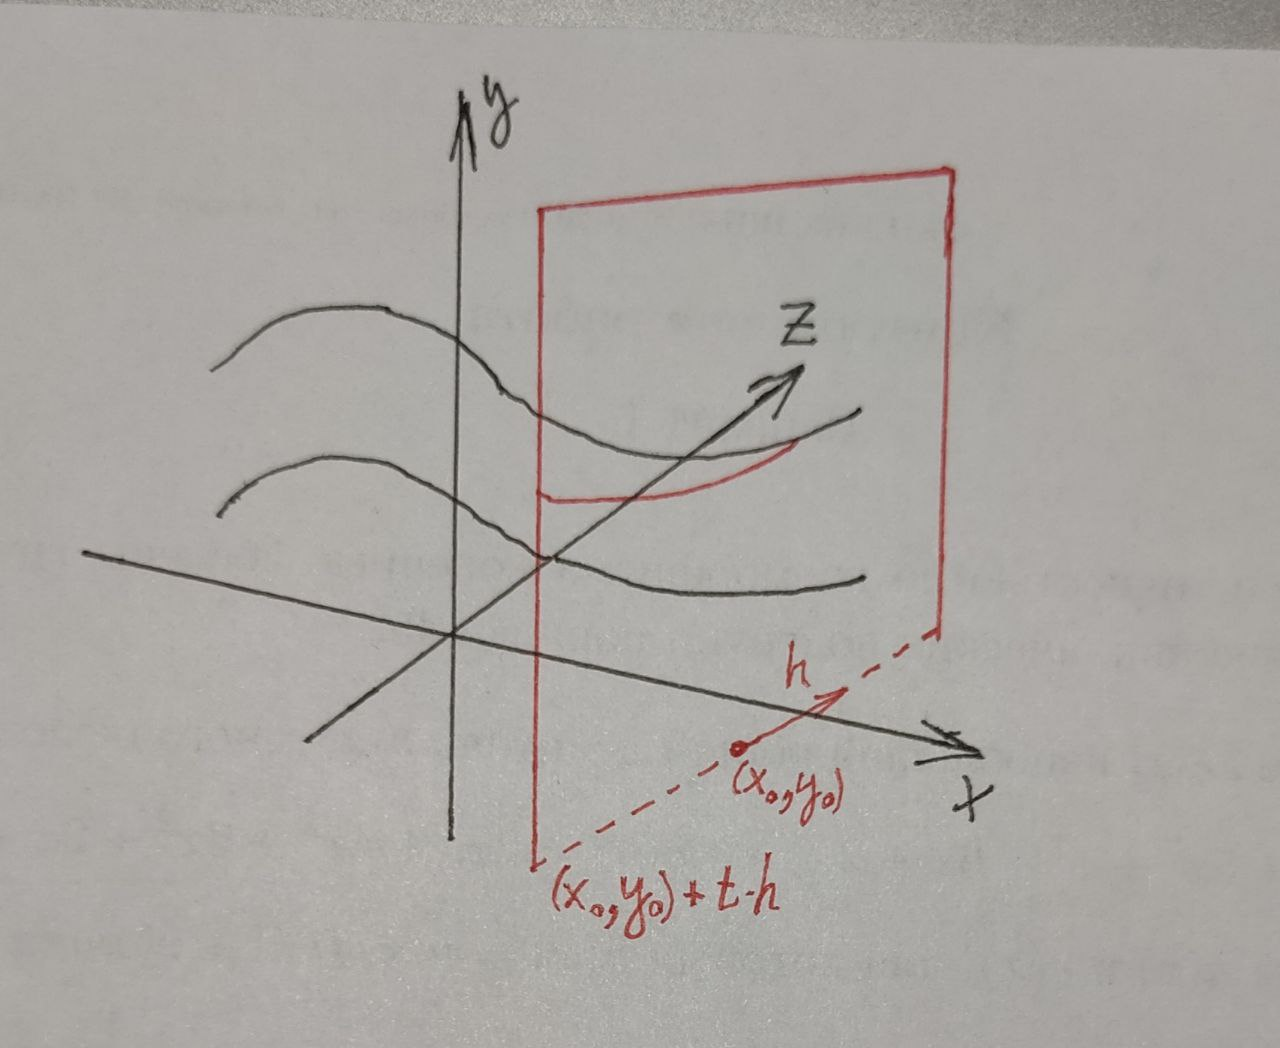
\includegraphics[width=0.4\textwidth]{img/lecture36/deriv}
    \end{center}
    
    Если мы зададим функцию в трёхмерном пространстве, то её график - это поверхность. Теперь если мы отметим точку $(x_0, y_0)$ и направление $h$ единичной длины (важно, иначе функция в сечении растянется или сожмётся), то $(x_0, y_0) + th$ заметает всю прямую. Тогда если мы посмотрим на значения функции в этих точках прямой, то мы сделаем сечение этой функции. Получим знакомую функцию в двумерной системе координат, у которой мы уже умеем находить производную. 
    
    \begin{example}
    	Пусть
    	\[ \displaystyle f(x, y) = \left\{{
    		\begin{matrix}
    			\frac{2xy}{x^2 + y^2}, (x, y) \neq (0, 0),  \\
    			0, (x, y) = (0, 0).
    		\end{matrix}
    	}\right. \]
    	Функция $f$ разрывна в нуле, а значит не дифференцируема, но в точке (0, 0) существуют обе частных производных. Действительно, если $x = r \cos{\phi}, y = r \sin{\phi}$, то функция $f(x, y) = \sin{2\phi}$.
    	Таким образом, $f(x, y)$ в любой окрестности точки (0, 0) принимает значения $\pm 1$, но $\deriv{f}{x} (0, 0) = \frac{d}{dx} (x, 0) = 0.$ Аналогично $\deriv{f}{y} (0, 0) = 0.$
    \end{example}
    
    \begin{explanation}
    	 \[ x = r \cos{\phi}, y = r \sin{\phi}, f(x, y) = \frac{2r^2 \sin{\phi} \cos{\phi}}{r^2} = \sin{2\phi} \]
    	 Значит значение функции в полярной системе координат не зависит от $r \Rightarrow$ в любой окрестности точки (0, 0) $\exists \phi$, в котором $f(x, y)$ принимает значения $\pm 1$, поэтому функция не непрерывна в нуле, тем более не дифференцируема (следствие 14.3).
    	 \begin{center}
    	 	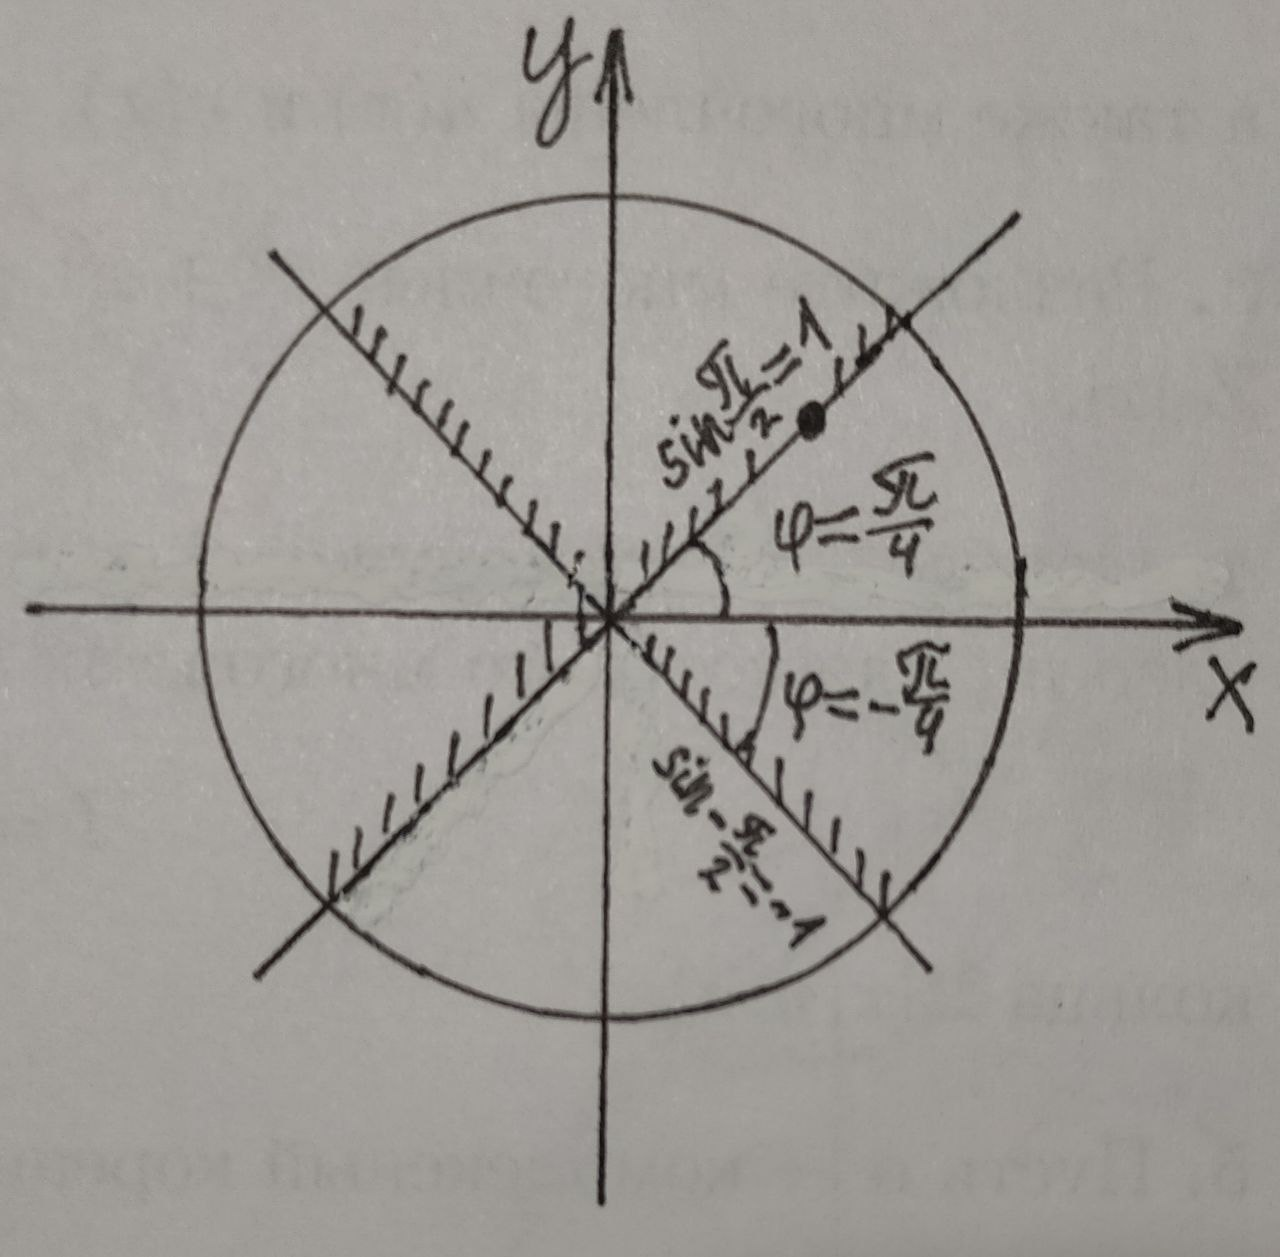
\includegraphics[width=0.4\textwidth]{img/lecture36/polar}
    	 \end{center}
    	 Производная вдоль $x$
    	 \[ \deriv{f}{x} = \lim_{t \to 0} \frac{f((0, 0) + t(1, 0)) - f(0, 0)}{t} = \lim_{t \to 0} \frac{f(t, 0) - f(0, 0)}{t} = \lim_{t \to 0} \frac{0 - 0}{t} = 0 \]
    	 Аналогично производная вдоль $y$ равна 0.
    \end{explanation}
    
    \section{Частная производная}
    
    \begin{definition}
    	Частной производной $\deriv{f}{x_j}$ функции $f : \R^k \rightarrow \R$ в точке $x = (x_1, ..., x_k)$ называется производная по направлению вектора $e_j$, т.е.
    	\[ \deriv{f}{x_j}(x) = \frac{d}{dt} f(x_1, ..., x_{j - 1}, t, x_{j + 1}, ..., x_k) \bigg|_{t = x_j}. \]
    \end{definition}
    
    \begin{explanation}
    	По определению производной по направлению 
    	\[ \deriv{f}{x_j}(x) = \deriv{f}{e_j}(x) = \frac{d}{dt}\bigg(f(x + te_j)\bigg) \bigg|_{t = 0} = \lim_{t \to 0} \frac{f(x + te_j) - f(x)}{t} = \]
    	\[ = \lim_{t \to 0} \frac{f(x_1, ..., x_{j - 1}, x_j + t, x_{j + 1}, ..., x_k) - f(x_1, ..., x_{j - 1}, x_j, x_{j + 1}, ..., x_k)}{t} = \]
    	\[ = \frac{d}{dy} f(x_1, ..., x_{j - 1}, y, x_{j + 1}, ..., x_k) \bigg|_{y = t + x_j} \]
    \end{explanation}
    
    \section{Градиент}
    
    \begin{mention}
    	При фиксированном базисе $e = \{e_1, ..., e_k\}$ в $\R^k$ линейные функционалы $dx_1, ..., dx_n$ оказываются сопряженным базисом к $e$, т.е. $dx_i(e_j) = \delta_{i,j}$. Таким образом,
    	\[ df = \deriv{f}{x_1} dx_1 + ... + \deriv{f}{x_k} dx_k. \]
    \end{mention}
    
    \begin{explanation}
	    $f: \R^k \rightarrow \R$
	    
	    $(e_1, ..., e_k) -$ фиксируем базис.
	    
	    $x_1 = \xi(x) = \xi(x_1, ..., x_k)$
	    
	    $dx_1 = d\xi$
	    
	    $\xi(x + h) - \xi(x) = x_1 + h_1 - x_1 = h_1 = d\xi(h) + \alpha(h) ||h||$
	    
	    Применим $df$ к $h = h_1 e_1 + ... + h_k e_k$ и воспользуемся линейностью.
	    \[ df(h) = df(e_1) h_1 + df(e_2) h_2 + ... + df(e_k) h_k = \deriv{f}{x_1}h_1 + ... + \deriv{f}{x_k}h_k = \deriv{f}{x_1} dx_1(h) + ... + \deriv{f}{x_k} dx_k(h) \]    
	    Тогда	    
	    \[ df = \deriv{f}{x_1} dx_1 + \deriv{f}{x_2} dx_2 + ... + \deriv{f}{x_k} dx_k \]
    \end{explanation}
    
    \begin{definition}
    	\underline{Градиентом} функции $f$ называется вектор $\nabla f := (\deriv{f}{x_1}, ..., \deriv{f}{x_n})$.
    \end{definition}
    
    \section{Свойства градиента}
    
    \begin{sentence}
    	Производная по направлению вектора $v$ равна
        \[ \deriv{f}{v} = \langle \nabla f(x), v \rangle. \]
    \end{sentence}
    
    \begin{proof}    
	    Из замечания 14.9
	    \[ \deriv{f}{v} = df(v) = \deriv{f}{x_1}v_1 + ... + \deriv{f}{x_k}v_k \Rightarrow \deriv{f}{v} = \langle \nabla f(x), v \rangle. \]
    \end{proof}
    
    \begin{lemma}
    	Если f дифференцируема в точке $x$ и $df \neq 0$, то наибольшее значение производной вдоль единичного вектора v (т.е. $||v|| = 1$) достигается на векторе $||\nabla f(x)||^{-1} \nabla f(x).$
    \end{lemma}
    
    \begin{proof}
    	По неравенству Коши-Буняковского
    	\[ |\langle \nabla f, v \rangle|^2 \leqslant ||\nabla f|| ||v|| \]
    	Максимум достигается при равенстве, то есть при $v = \frac{\nabla f}{||\nabla f||}$
    \end{proof}
    
    \newpage
    
    \section*{Лекция 37: Частные производные высокого порядка}
    
    \section{Множество уровня}
    
    \begin{definition}
    	\underline{Множеством уровня} называется
    	\[ \gamma(h) = \{(x_1, ..., x_n) \text{ } | \text{ } \phi(x_1, ..., x_n) = h\}. \]
    \end{definition}
    
    \begin{sentence}
    	Градиент функции $\phi$ в точке $\vec{x}^0$ перпендикулярен её множеству уровня, проходящей через эту точку.
    \end{sentence}
    
    Пока без доказательства
    
    \section{Матрица Якоби}
    
    \begin{mention}
    	В случае отображения $f : \R^k \rightarrow \R^m$ при фиксированных базисах $e$ и $e'$ в $\R^k$ и в $\R^m$ соответственно, компоненты матрицы дифференциала $df$ имеют $a_{i, j} = \deriv{f_i}{x_j} (x)$, т.е. по строчкам написаны градиенты $\nabla f_i(x).$
    \end{mention}
    
    \begin{definition}
    	При фиксированных базисах $e$ в $\R^k$ и $e'$ в $\R^m$ матрицу, соответствующую линейному отображению $df$, называют \underline{матрицей Якоби} отображения $f$ в точке $x$ и обозначают $J_f (x)$.
    \end{definition}
    
    \section{Достаточное условие дифференцируемости}
    
    \begin{theorem}
    	Если все частные производные $\deriv{f}{x_j}$ существуют в окрестности точки $x_0$ и непрерывны в этой точке, то $f$ — дифференцируема в точке $x_0$.
    \end{theorem}
    
    \begin{proof}
    	Индукция по числу переменных.
    	
    	$k = 1.$ У функции от одной переменной одна частная производная и она равна производной.
    	
    	Пусть утверждение верно для некоторого $k$, докажем для $k + 1$.
    	
    	$a = (a_1, a_2, ..., a_{k + 1})$
    	\[ f(a_1 + h_1, ..., a_{k + 1} + h_{k + 1}) - f(a) = f(a_1 + h_1, ..., a_k + h_k, a_{k + 1} + h_{k + 1}) - \]
    	\[ - f(a_1 + h_1, .., a_k + h_k, a_{k + 1}) + f(a_1 + h_1, ..., a_k + h_k, a_{k + 1}) - f(a) \]
    	Пусть
    	\[ \sigma = f(a_1 + h_1, ..., a_k + h_k, a_{k + 1} + h_{k + 1}) - f(a_1 + h_1, .., a_k + h_k, a_{k + 1}) \]
    	\[ \rho = f(a_1 + h_1, ..., a_k + h_k, a_{k + 1}) - f(a) \]
    	Считаем, что функция $\rho$ от $k$ переменных и применяем предположение индукции. Расписываем определение дифференцируемости и формулы дифференциала через частные производные:
    	\[ \rho = f(a) + \deriv{f}{x_1}(a)h_1 + ... + \deriv{f}{x_k}(a)h_k + \alpha(h)||h|| - f(a) = \deriv{f}{x_1}(a)h_1 + ... + \deriv{f}{x_k}(a)h_k + o(||h||) \]
    	(Важные моменты: $f(a + h) \to f(a)$ при $h \to 0$; у $h$ всего $k + 1$ координат, поэтому если $h \to 0$, то его первые $k$ координат тоже стремятся к нулю)
    	
    	По теореме Лангранжа $\exists \xi: 0 < \xi < h_{k + 1}$
    	\[ \sigma = \deriv{f}{x_{k + 1}}(a_1 + h_1, ..., a_k + h_k, a_{k + 1} + \xi) h_{k + 1} = \deriv{f}{x_{k + 1}}(a)h_{k + 1} - \deriv{f}{x_{k + 1}}(a)h_{k + 1} + \]
    	\[ + \deriv{f}{x_{k + 1}}(a_1 + h_1, ..., a_k + h_k, a_{k + 1} + \xi)h_{k + 1} = \deriv{f}{x_{k + 1}}(a)h_{k + 1} + \bigg(-\deriv{f}{x_{k + 1}}(a) + \]
    	\[ + \deriv{f}{x_{k + 1}}(a_1 + h_1, ..., a_k + h_k, a_{k + 1} + \xi)\bigg)h_{k + 1} \]
    	Пользуясь непрерывностью частных производных и тем, что $h_i \to 0$, $0 < \xi < h_{k + 1}$, получаем, что
    	\[ \bigg(-\deriv{f}{x_{k + 1}}(a) + \deriv{f}{x_{k + 1}}(a_1 + h_1, ..., a_k + h_k, a_{k + 1} + \xi)\bigg) = \alpha(h) \]
    	\[ \alpha(h)||h|| = o(||h||) \Rightarrow \rho + \sigma = \deriv{f}{x_1}(a)h_1 + ... + \deriv{f}{x_k}(a)h_k + \deriv{f}{x_{k + 1}}(a) + o(||h||) \]
    	Хочется заметить, что когда мы используем теорему Лангранжа необходимо, чтобы функция не только была дифференцируема, но и непрерывна на каком-то отрезке. Наша функция дифференцируема в некоторой окрестности точки $a$, поэтому можно взять точки $h_k$, которые лежат внутри этой окрестности. Для того, чтобы добиться непрерывности в каждой точке, возьмём окрестность поменьше (с включённой границей), так, чтобы эти точки $h_k$ остались всё ещё в окрестности.
    	\begin{center}
    		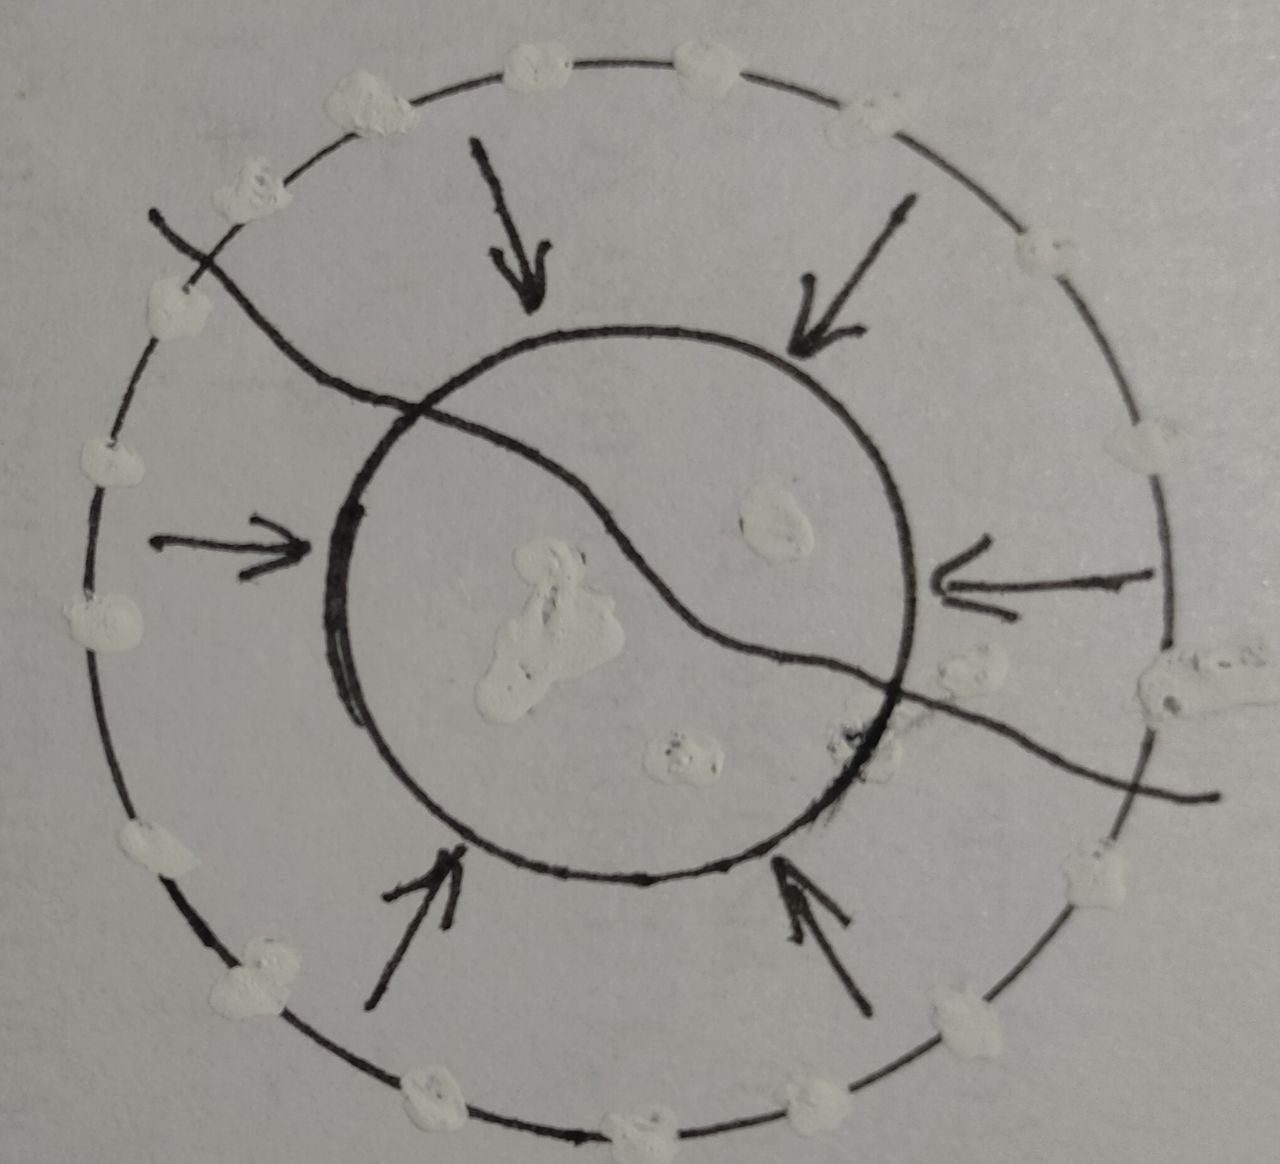
\includegraphics[width=0.4\textwidth]{img/lecture37/circle}
    	\end{center}
    \end{proof}
    
    \section{Частные производные высокого порядка}
    
    \begin{definition}
    	Пусть $f : \R^k \rightarrow \R$ и предположим, что в некоторой окрестности $B_r(x_0)$ точки $x_0$ существует частная производная $\pdv{f}{x_j}$. Если функция $x \mapsto \pdv{f}{x_j}$ в точке $x_0$ имеет частную производную по переменной $x_i$, то эта частная производная $\pdv{x_i}(\pdv{f}{x_j})(x_0)$ называется частной производной второго порядка по переменным $x_j$ и $x_i$ и обозначается $\frac{\partial^2 f}{\partial x_i \partial x_j}(x_0)$. 
    	    	
    	Частная производная порядка k определяется рекурсивно:
    	\[ \frac{\partial^k f}{\partial x_{i_1} \cdot \cdot \cdot \partial x_{i_k}} = \pdv{x_{i_1}}(\frac{\partial^{k - 1} f}{\partial x_{i_2} \cdot \cdot \cdot \partial x_{i_k}}). \]
    \end{definition}
    
    \begin{mention}
    	Частные производные $\frac{\partial^2 f}{\partial x_i \partial x_j}$ и $\frac{\partial^2 f}{\partial x_j \partial x_i}$, вообще говоря, могут не совпадать!
    \end{mention}
    
    \section{Теорема Шварца}
    
    \begin{theorem}[Шварц]
    	Пусть смешанные частные производные $\frac{\partial^2 f}{\partial x \partial y}$ и $\frac{\partial^2 f}{\partial y \partial x}$ существуют в окрестности точки $(x_0, y_0)$ и непрерывны в этой точке. Тогда их значения в точке $(x_0, y_0)$ совпадают.
    \end{theorem}
    
    \begin{proof}
    	Рассмотрим
    	\[ F(t, s) = f(x_0 + t, y_0 + s) - f(x_0 + t, y_0) - f(x_0, y_0 + s) + f(x_0, y_0) \]
    	Пусть
    	\[ \psi(\tau) = f(x_0 + \tau, y_0 + s) - f(x_0 + \tau, y_0) \]
    	По теореме Лагранжа $\exists c: 0 < c < t$
    	\[ F(t, s) = \psi(t) - \psi(0) = \psi'(c) \cdot t \]
    	\[ \psi'(c) = \deriv{f}{x}(x_0 + c, y_0 + s) - \deriv{f}{x}(x_0 + c, y_0) \]
    	\[ \phi(u) = \deriv{f}{x}(x_0 + c, y_0 + u) \]
    	
    	По теореме Лагранжа $\exists d: 0 < d < s$
    	\[ \psi'(c) = \phi(s) - \phi(0) = \phi'(d) \cdot s \]
    	\[ \phi'(d) = \frac{\partial^2 f}{\partial y \partial x}(x_0 + c, y_0 + d), 0 < d < s, 0 < c < t \]
    	Для всех $t$ и $s$ из достаточно малой окрестности 0
    	\[ F(t, s) = \frac{\partial^2 f}{\partial y \partial x}(x_0 + c, y_0 + d) \cdot t \cdot s, 0 < d < s, 0 < c < t \]
    	Если перегруппировать слагаемые иначе, получим
    	\[ F(t, s) = \frac{\partial^2 f}{\partial x \partial y} \big(x_0 + \widetilde{c}, y_0 + \widetilde{d} \big) \cdot t \cdot s, 0 < \widetilde{d} < s, 0 < \widetilde{c} < t \]
    	следовательно
    	\[ \frac{\partial^2 f}{\partial x \partial y} \big(x_0 + \widetilde{c}, y_0 + \widetilde{d} \big) = \frac{\partial^2 f}{\partial y \partial x} (x_0 + c, y_0 + d) \]
    	\[ t \to 0 \Rightarrow c \to 0, \widetilde{c} \to 0 \]
    	\[ s \to 0 \Rightarrow d \to 0, \widetilde{d} \to 0 \]
    	В силу непрерывности смешанных производных
    	\[ \frac{\partial^2 f}{\partial x \partial y} = \frac{\partial^2 f}{\partial y \partial x} \]
    \end{proof}

    \section{Теорема Юнга}
    
    \begin{theorem}[Юнг]
    	Пусть $f$ - дифференцируема в окрестности точки $(x_0, y_0)$, а её частные производные $\pdv{f}{x}$ и $\pdv{f}{y}$ дифференцируемы в точке $(x_0, y_0)$. Тогда смешанные частные производные $\frac{\partial^2 f}{\partial x \partial y}$ и $\frac{\partial^2 f}{\partial y \partial x}$ в точке $(x_0, y_0)$ совпадают.
    \end{theorem}
    
    \begin{proof}
    	Не ограничивая общности, будем считать, что $(x_0, y_0) = (0, 0)$. Рассмотрим функцию
    	\[ F(t, t) = f(t, t) - f(0, t) - f(t, 0) + f(0, 0). \]
    	Применяя теорему Лагранжа к функции $g(u) = f(t, u) - f(0, u)$, получаем
    	\[ F(t, t) = g(t) - g(0) = g'(\xi)t = \bigg(\deriv{f}{y}(t, \xi) - \deriv{f}{y}(0, \xi)\bigg)t. \]
    	Дифференцируемость $\deriv{f}{y}$ в точке (0, 0) означает, что
    	\[ \deriv{f}{y}(x, y) = \deriv{f}{y}(0, 0) + \frac{\partial^2 f}{\partial x \partial y}(0, 0)x + \frac{\partial^2 f}{\partial y^2}(0, 0)y + o(\sqrt{x^2 + y^2}). \]
    	Таким образом,
    	\[ \deriv{f}{y}(t, \xi) = \deriv{f}{y}(0, 0) + \frac{\partial^2 f}{\partial x \partial y}(0, 0)t + \frac{\partial^2 f}{\partial y^2}(0, 0)\xi + o(\sqrt{t^2 + \xi^2}). \]
    	и
    	\[ \deriv{f}{y}(0, \xi) = \deriv{f}{y}(0, 0) + \frac{\partial^2 f}{\partial y^2}(0, 0)\xi + o(\xi). \]
    	Т. к. $0 \leqslant \xi \leqslant t$, то $o(\sqrt{t^2 + \xi^2}) = o(t)$ (т. к. $\sqrt{t^2 + \xi^2} \leqslant \sqrt{2}t$) и $o(\xi) = o(t)$. Таким образом,
    	\[ F(t, t) = \frac{\partial^2 f}{\partial x \partial y}(0, 0)t^2 + o(t^2). \]
    	Аналогично, обозначив $g(u) = f(u, t) - f(u, 0)$, получим
    	\[ F(t, t) = \frac{\partial^2 f}{\partial y \partial x}(0, 0)t^2 + o(t^2). \]
    	Приняв полученные выражения, поделив на $t^2$ и устремив $t$ к нулю, получаем
    	\[ \frac{\partial^2 f}{\partial x \partial y}(0, 0) = \frac{\partial^2 f}{\partial y \partial x}(0, 0). \]
    \end{proof}
    
    \begin{mention}
    	Условия теорем Юнга и Шварца не следуют друг из друга.
    \end{mention}
    
    \section{Дифференцируемость (m + 1) раз}
    
    \begin{definition}
    	Пусть $f : \R^n \rightarrow \R$ дифференцируема в окрестности точки $a$. Говорят, что $f$ дважды дифференцируема в точке $a$, если все её частные производные $\pdv{f}{x_i}$ дифференцируемы в точке $a$. 
    	
    	Пусть $f$ - $m$ раз дифференцируема в окрестности точки $a$. Говорят, что $f$ дифференцируема $(m + 1)$ раз в точке $a$, если все частные производные $m$-того порядка $\frac{\partial^m f}{\partial x_{i_1} ... \partial x_{i_m}}$ дифференцируемы в точке $a$.
    \end{definition}
    
    \begin{corollary}
    	Если $f$ - $m$ раз дифференцируема в точке $a$, то значения производных порядка $m$  $\frac{\partial^m f}{\partial x_{i_1} ... \partial x_{i_m}}(a)$ не зависят от порядка дифференцирования.
    \end{corollary}
    
    \begin{proof}
    	База индукции для $m = 2$: теорема Юнга.
    	
    	Переход: рассмотрим производную порядка $m + 1$.
    	\[ \deriv{}{x_{k_{m + 1}}} \bigg(\frac{\partial^m f}{\partial x_{k_m} ... \partial x_{k_1}}\bigg) \]
    	По предположению индукции внутри скобок можно дифференцировать в любом порядке. Поскольку функция $\frac{\partial^m f}{\partial x_{k_m} ... \partial x_{k_1}}$ дифференцируема, то по теореме Юнга мы можем переставлять частную производную по переменной $x_{k_{m + 1}}$ в любое место.
    \end{proof}
    
    \newpage
    
    \section*{Лекция 38: Правила дифференцирования}
    
    \section{Дифференциалы высоких порядков}
    
    Предположим, что $f : \R^k \rightarrow \R$ - дифференцируема в окрестности точки $a$ и предположим, что ее частные производные $\pdv{f}{x_j}$ дифференцируемы в точке $a$. Тогда при каждом $h \in \R^k$ возникает функция $x \mapsto df|_x (h) = \deriv{f}{x_1}(x) h_1 + ... + \deriv{f}{x_k}(x) h_k$, дифференцируема в точке $a$. Ее дифференциал
    \[ d(df(h))|_a (q) = \bigg(\sum_{j = 1}^k \frac{\partial^2 f}{\partial x_j \partial x_1}(a) q_j \bigg) h_1 + ... + \bigg(\sum_{j = 1}^k \frac{\partial^2 f}{\partial x_j \partial x_k}(a) q_j \bigg) h_k. \]
    Т.е. получена билинейная форма $d(df(h))|_a (q) = \sum_{i, j = 1}^k \frac{\partial^2 f}{\partial x_j \partial x_i}(a) q_j h_i$. Эта билинейная форма оказывается симметричной по теореме Юнга, а т.к. симметричная билинейная форма однозначно задается своей квадратичной формой
    \[ d(df(h))|_a (h) = \sum_{i, j = 1}^k \frac{\partial^2 f}{\partial x_j \partial x_i}(a) h_j h_i = \sum_{i, j = 1}^k \frac{\partial^2 f}{\partial x_j \partial x_i}(a) dx_j(h) dx_i(h),\]
    то эту квадратичную форму $d^2 f := \sum_{i,j = 1}^k \frac{\partial^2 f}{\partial x_j \partial x_i}(a) dx_j dx_i$ и называют \underline{вторым диф-} \underline{ференциалом} функции $f$.
    
    \begin{definition}
    	Если f — $n$ раз дифференцируема в точке a, то
    	\[  d^n f|_a := \sum_{1 \leqslant j_1, ..., j_n \leqslant k???} \frac{\partial^n f}{\partial x_{j_1} ... \partial x_{j_n}}(a) dx_{j_1} ... dx_{j_n}. \]
    	Последняя запись означает лишь то, что при вычислении $n$-го дифференциала на векторе $h \in \R^k$ надо воспользоваться линейностью, а
    	\[ [dx_{j_1} ... dx_{j_n}](h) := dx_{j_1}(h) ... dx_{j_n}(h) = h_{j_1} ... h_{j_n}. \]
    \end{definition}
    
    \section{Правила дифференцирования}
    
    \begin{theorem}
    	Пусть функции $f, g : \R^k \rightarrow \R$ дифференцируемы в некоторой точке $x$. Тогда, для произвольных чисел $a, b \in \R$, функции $af + bg$ и $fg$ дифференцируемы в точке $x$ и $d(af + bg) = adf + bdg$ и $d(fg) = fdg + gdf$.
    \end{theorem}
    
    \begin{proof}
    	$\alpha(h), \beta(h), \gamma(h) \to 0$ при $h \to 0$
    	\begin{enumerate}
    		\item Здесь доказываем в общем случае, т. е. для функций $f, g : \R^k \rightarrow \R^n$.
    	    \[ f(x + h) - f(x) = df|_x(h) + \alpha(h)||h|| \]
    	    \[ g(x + h) - g(x) = dg|_x(h) + \beta(h)||h|| \]
    	    \[ (af + bg)(x + h) - (af + bg)(x) = af(x + h) + bg(x + h) - af(x) - bg(x) = \]
    	    \[ = a(df|_x(h) + \alpha(h)||h||) + b(dg|_x(h) + \beta(h)||h||) = a \cdot df(h) + b \cdot dg(h) + (\alpha(h) + \beta(h))||h|| = \]
    	    \[ = a \cdot df(h) + b \cdot dg(h) + \gamma(h)||h|| \]
    	    \item 
    	    \[ fg(x + h) - fg(x) = f(x + h)g(x + h) - f(x)g(x) = f(x + h)g(x + h) - f(x + h)g(x) + \] \[ + f(x + h)g(x) - f(x)g(x) = f(x + h)(g(x + h) - g(x)) + g(x)(f(x + h) - f(x)) = \]
    	    \[ = f(x + h) (dg|_x(h) + \beta(h)||h||) + g(x)(df|_x(h) + \alpha(h)||h||) = (*) \]
    	    Функция $f$ дифференцируема $\Rightarrow$ непрерывна в точке $x$ и $h \to 0$. Тогда
    	    \[ (*) = (f(x) + o(1)) (dg|_x(h) + \beta(h)||h||) + g(x)(df|_x(h) + \alpha(h)||h||) = f(x)dg|_x(h) + \]
    	    \[ + f(x)\beta(h)||h|| + o(1)dg|_x(h) + o(1)\beta(h)||h|| + g(x)df|_x(h) + g(x) \alpha(h)||h|| = \]
    	    \[ = f(x) dg|_x(h) + g(x) df|_x(h) + \gamma(h) ||h||. \]
    	    $f(x)$ и $g(x)$ - константы $\Rightarrow f(x)\beta(h)||h|| = \gamma(h) ||h||$ и $g(x) \alpha(h)||h|| = \gamma(h) ||h||$
    	     
    	    $||dg|_x(h)|| \leqslant C||h||$ (см. конец замечания 14.2) $\Rightarrow o(1)dg|_x(h) = \gamma(h) ||h||$
    	    
    	    $o(1)\beta(h)||h|| = \gamma(h) ||h||$
    	\end{enumerate}
    \end{proof}
    
    \section{Дифференцирование сложной функции}
    
    \begin{theorem}
    	Пусть $f : \R^k \rightarrow \R^m$, $g : \R^m \rightarrow \R^n$, причем отображение $f$ дифференцируемо в точке $a$, отображение $g$ дифференцируемо в точке $f(a)$. Тогда отображение $g \circ f$ дифференцируемо в точке $a$ и $d(g \circ f)|_a = dg|_{f(a)} \circ df|_a$.
    \end{theorem}
    
    \begin{proof}
    	$h \in \R^k, q \in \R^m$
    	\[ f(a + h) = f(a) + df|_a(h) + \alpha(h) ||h|| \]
    	\[ g(f(a) + q) = g(f(a)) + dg|_{f(a)}(q) + \beta(q)||q|| \]
    	\[ g(f(a + h)) - g(f(a)) = g(f(a) + (f(a + h) - f(a))) - g(f(a)) = (*) \]
    	Функция $f$ - дифференцируема $\Rightarrow$ непрерывна $\Rightarrow$ при $h \to 0$, $f(a + h) - f(a) \to 0 \Rightarrow q \to 0$, поэтому
    	\[ (*) = g(f(a)) + dg|_{f(a)}(f(a + h) - f(a)) + \beta(f(a + h) - f(a))||f(a + h) - f(a)|| - g(f(a)) = \]
    	\[ = dg|_{f(a)}(df|_a(h) + \alpha(h)||h||) + \gamma(h)||h|| = (**) \]
    	Докажем, что 
    	\[ \gamma(h) = \beta(f(a + h) - f(a))\frac{||f(a + h) - f(a)||}{||h||}, \]
    	где $\gamma(h)$ - бесконечно малая функция.
    	Функция $f$ - дифференцируема $\Rightarrow$ непрерывна $\Rightarrow$ при $h \to 0$, $f(a + h) - f(a) \to 0$
    	\[ \frac{||f(a + h) - f(a)||}{||h||} = ||df(\frac{h}{||h||}) + \alpha(h)|| \leqslant \text{(неравенство треугольника)} \]
    	\[ \leqslant ||df\bigg(\frac{h}{||h||}\bigg)|| + ||\alpha(h)|| \]
    	По замечанию 14.2 $||df\big(\frac{h}{||h||}\big)|| \leqslant C||\frac{h}{||h||}|| = C$
    	
    	Далее продолжаем преобразования
    	\[ (**) = dg|_{f(a)} \circ df|_a{(h)} + ||h||dg|_{f(a)}(\alpha(h)) + \gamma(h)||h|| = (***) \]
    	По замечанию 14.2 $||h||dg|_{f(a)}(\alpha(h)) \leqslant ||h||C||\alpha(h)|| \to 0$
    	\[ (***) = dg|_{f(a)} \circ df|_a{(h)} + \gamma_2(h)||h|| \]
    	$dg|_{f(a)} \circ df|_a{(h)}$ означают композицию двух линейных отображений.
    \end{proof}
    
    \begin{mention}
    	Поясним запись $d(g \circ f)|_a = dg|_{f(a)} \circ df|_a$. Здесь $df|_a : \R^k \rightarrow \R^m$ есть линейное отображение и $dg|_{f(z)} : \R^m \rightarrow \R^n$ есть линейное отображение. Тогда их композиция $dg|_{f(a)} \circ df|_a : \R^k \rightarrow \R^n$ есть линейное отображение, действующее по правилу $dg|_{f(a)} \circ df|_a (h) = dg|_{f(a)} (df|_a (h))$.
    \end{mention}
    
    \begin{mention}
    	Матрица Якоби композиции функций $g \circ f$ в точке $a$ равняется произведению матриц Якоби отображения $f$ в точке $a$ и отображения $g$ в точке $f(a)$. В частности, при $n = 1$, для функции $g(x_1, ..., x_m)$ и отображения
    	\[ f(y_1, ..., y_k) = (f_1(y_1, ..., y_k), ..., f_m(y_1, ..., y_k)), \]
    	во-первых, выполнено:
    	\[ \frac{\partial (g \circ f)}{\partial y_j}(a) = \frac{\partial g}{\partial x_1}(f(a)) \frac{\partial f_1}{\partial y_j}(a) + ... + \frac{\partial g}{\partial x_m}(f(a)) \frac{\partial f_m}{\partial y_j}(a). \]
    	Во-вторых, выполнено так называемое свойство инвариантности 1-го дифференциала: $dg = \pdv{g}{x_1}dx_1 + ... + \pdv{g}{x_m}dx_m$, где нам не важно, являются ли $dx_1, ..., dx_m$ - дифференциалами независимых переменных или же являются дифференциалами некоторых функций $x_j = f_j(y_1, ..., y_k)$.
    \end{mention}
    
    \begin{explanation}
    	\begin{enumerate}
    		\item При композиции линейных отображений их матрицы перехода перемножаются. Для каждой функции такие матрицы будут иметь вид
    		\[ J_f = \begin{pmatrix}
    			\deriv{f_1}{x_1} & \deriv{f_1}{x_2} & ... & \deriv{f_1}{x_k} \\
    			\deriv{f_2}{x_1} & \deriv{f_2}{x_2} & ... & \deriv{f_2}{x_k} \\
    			... & ... & ... & ... \\
    			\deriv{f_m}{x_1} & \deriv{f_m}{x_2} & ... & \deriv{f_m}{x_k}
    		\end{pmatrix},
    		J_g = \begin{pmatrix}
    			\deriv{g}{f_1} & \deriv{g}{f_2} & ... & \deriv{g}{f_m} \\
    		\end{pmatrix}. \]
    		Тогда матрица перехода композиции функций будет равна $J_g J_f$.
    		\item С одной стороны,
    		\[ dg = \deriv{g}{f_1} df_1 + ... + \deriv{g}{f_m} df_m \]
    		С другой стороны,
    		\[ dg(f) = \pdv{(g \circ f)}{x_1}dx_1 + ... + \pdv{(g \circ f)}{x_k}dx_k = \sum_{i = 1}^k \deriv{(g \circ f)}{x_i} \; dx_i = \sum_{i = 1}^k \bigg(\sum_{j = 1}^m \deriv{g}{f_j} \deriv{f_j}{x_i} \bigg) \; dx_i = \]
    		\[ = \sum_{j = 1}^m \bigg(\sum_{i = 1}^k \deriv{g}{f_j} \deriv{f_j}{x_i} \; dx_i \bigg) = \sum_{j = 1}^m \deriv{g}{f_j} \bigg(\sum_{i = 1}^k \deriv{f_j}{x_i} \; dx_i \bigg) = \sum_{j = 1}^m \deriv{g}{f_i} df_j \]
    	\end{enumerate}
    \end{explanation}
    
    \begin{example}
    	Пусть $f(x, y) = \phi(u, v, w)$, где $u = xy, v = x + y, w = x - y$. Тогда
    	\[ df = \pdv{\phi}{u} du + \pdv{\phi}{v} dv + \pdv{\phi}{w} dw = \frac{\partial \phi}{\partial u} d(xy) + \frac{\partial \phi}{\partial v} d(x + y) + \frac{\partial \phi}{\partial w} d(x - y) = \]
    	\[ = \frac{\partial \phi}{\partial u}(xdy + ydx) + \frac{\partial \phi}{\partial v}(dx + dy) + \frac{\partial \phi}{\partial w}(dx - dy). \]
    	В частности, $\pdv{f}{x} = y \pdv{\phi}{u} + \pdv{\phi}{v} + \pdv{\phi}{w}$ и $\pdv{f}{y} = x \pdv{\phi}{u} + \pdv{\phi}{v} - \pdv{\phi}{w}$.
    \end{example}
    
    \section{Дифференциал обратного отображения}
    
    \begin{theorem}
    	Пусть $f : \R^k \rightarrow \R^k$ - есть непрерывная биекция между окрестностями $U(a)$ и $V(f(a))$, причем обратное отображение $f^{-1} : V (f(a)) \rightarrow U(a)$ также непрерывно (т. е. $f$ -	гомеоморфизм между $U(a)$ и $V(f(a))$). Предположим, что $f$ - дифференцируемо в точке $a$ и $df$ - обратимое линейное
    	отображение. Тогда $f^{-1}$ - дифференцируемо в точке $f(a)$ и $df^{-1}|_{f(a)}	= (df|_a)^{-1}$.
    \end{theorem}
    
    \begin{proof}
    	Достаточно доказать, что такой предел равен 0.
    	\[ \lim_{q \to 0} \frac{||f^{-1}(f(a) + q) - f^{-1}(f(a)) - (df|_a)^{-1}(q)||}{||q||} \]
    	\[ h = f^{-1}(f(a) + q) - f^{-1}(f(a)), h \to 0 \Leftrightarrow q \to 0 \]
    	\[ h = f^{-1}(f(a) + q) - a \Rightarrow q = f(a + h) - f(a) \]
    	$f$ дифференцируемо в точке $a$, поэтому
    	\[ \lim_{h \to 0} \frac{||h - (df|_a)^{-1}(f(a + h) - f(a))||}{||f(a + h) - f(a)||} = \lim_{h \to 0} \frac{||h - (df|_a)^{-1}(df|_a(h) + \alpha(h)||h||)||}{||f(a + h) - f(a)||} = \]
    	Пользуемся линейностью дифференциала и тем, что по замечанию 14.2 $(df|_a)^{-1}(\alpha(h)) \leqslant C||\alpha(h)||$
    	\[ = \lim_{h \to 0} \frac{||\alpha(h)|| \cdot ||h||}{||df(h) + \alpha(h)||h||||} = \lim_{h \to 0} \frac{||\alpha(h)||}{||df\big(\frac{h}{||h||}\big) + \alpha(h))||} \]
    	Теперь отдельно оценим знаменатель. $p$ - вектор $\Rightarrow$ по замечанию 14.2
    	\[ ||(df)^{-1}(p)|| \leqslant C ||p|| \]
    	Пусть $p = df(h)$.
    	\[ ||(df)^{-1}(df(h))|| \leqslant C||df(h)|| \]
    	\[ ||h|| C_2 \leqslant ||df(h)|| \]
    	Таким образом, применяя неравенство треугольника,
    	\[ ||df\bigg(\frac{h}{||h||}\bigg) + \alpha(h)|| \geqslant ||df\bigg(\frac{h}{||h||}\bigg)|| - ||\alpha(h)|| \geqslant C - ||\alpha(h)|| \Rightarrow \lim_{h \to 0} \frac{||\alpha(h)||}{||df\big(\frac{h}{||h||}\big) + \alpha(h))||} = 0 \]
    \end{proof}
    
    \newpage
    
    \chapter{Экстремумы функций многих переменных}
    
    \section*{Лекция 39: Формула Тейлора и экстремум}
    
    \section{Формула Тейлора с остаточным членом в интегральной форме}
    
    \begin{theorem}[Формула Тейлора с остаточным членом в интегральной форме]
    	Если $f: \R \rightarrow \R$ непрерывно дифференцируема $m + 1$ раз на отрезке $[a, x]$, то
    	\[ f(x) = f(a) + f'(a)(x - a) + ... + \frac{1}{m!}f^{(m)}(a)(x - a)^m + \frac{1}{m!} \int_a^x (x - t)^m f^{(m + 1)}(t) \; dt \]
    \end{theorem}
    
    \begin{proof}
    	База: $m = 0$.
    	\[ f(x) = f(a) + \int_a^x f'(t) \; dt = f(a) + f(x) - f(a) = f(x) \]
    	Переход:
    	\[ R_m = \frac{1}{m!} \int_a^x (x - t)^m f^{(m + 1)}(t) \; dt = -\frac{1}{(m + 1)!} \int_a^x f^{(m + 1)}(t) \; d(x - t)^{m + 1} = \]
    	\[ = -\frac{(x - t)^{m + 1}}{(m + 1)!} f^{(m + 1)}(t)\bigg|_a^x + \frac{1}{(m + 1)!} \int_a^x (x - t)^{m + 1} f^{(m + 2)}(t) \; dt = \]
    	\[ = \frac{(x - a)^{m + 1}}{(m + 1)!} f^{(m + 1)}(a) + R_{m + 1} \]
    \end{proof}
    
    \begin{corollary}
    	Справедливо следующее равенство:
    	\[ e^x = \sum_{n = 0}^{\infty} \frac{x^n}{n!}, x \in \R. \]
    \end{corollary}
    
    \begin{proof}
    	\[ \bigg|e^x - \sum_{k = 0}^m \frac{x^k}{k!}\bigg| = \bigg|\frac{1}{m!} \int_0^x (x - t)^m e^t \; dt\bigg| = (*) \]
    	Пользуемся следующей оценкой
    	\[ \bigg|\int_a^b \phi(x) \; dx\bigg| \leqslant \sup_{x \in [a, b]} |\phi(x)|(b - a) \]
    	При $x \geqslant 1$
    	\[ (*) \leqslant \bigg|\frac{x^{m + 1} e^x}{m!}\bigg| \to 0 \text{ при } m \to \infty \text{ и фиксированном x} \]
    	При $x < 1$
    	\[ (*) \leqslant \bigg|\frac{e^x}{m!}\bigg| \to 0 \]
    \end{proof}
    
    \section{Формула Тейлора}
    
    \begin{lemma}
    	Пусть функция $f: \R \rightarrow \R$ $m$ раз дифференцируема в окрестности точки $a \in \R^k$. Рассмотрим функцию $\phi(t) := f(a + th)$. Тогда $\phi$ $m$ раз дифференцируема в окрестности точки нуль и $\phi^{(m)}(t) = d^mf|_{a + th}(h)$.
    \end{lemma}
    
    \begin{proof}
    	База индукции: $m = 1$.
    	\begin{center}
    		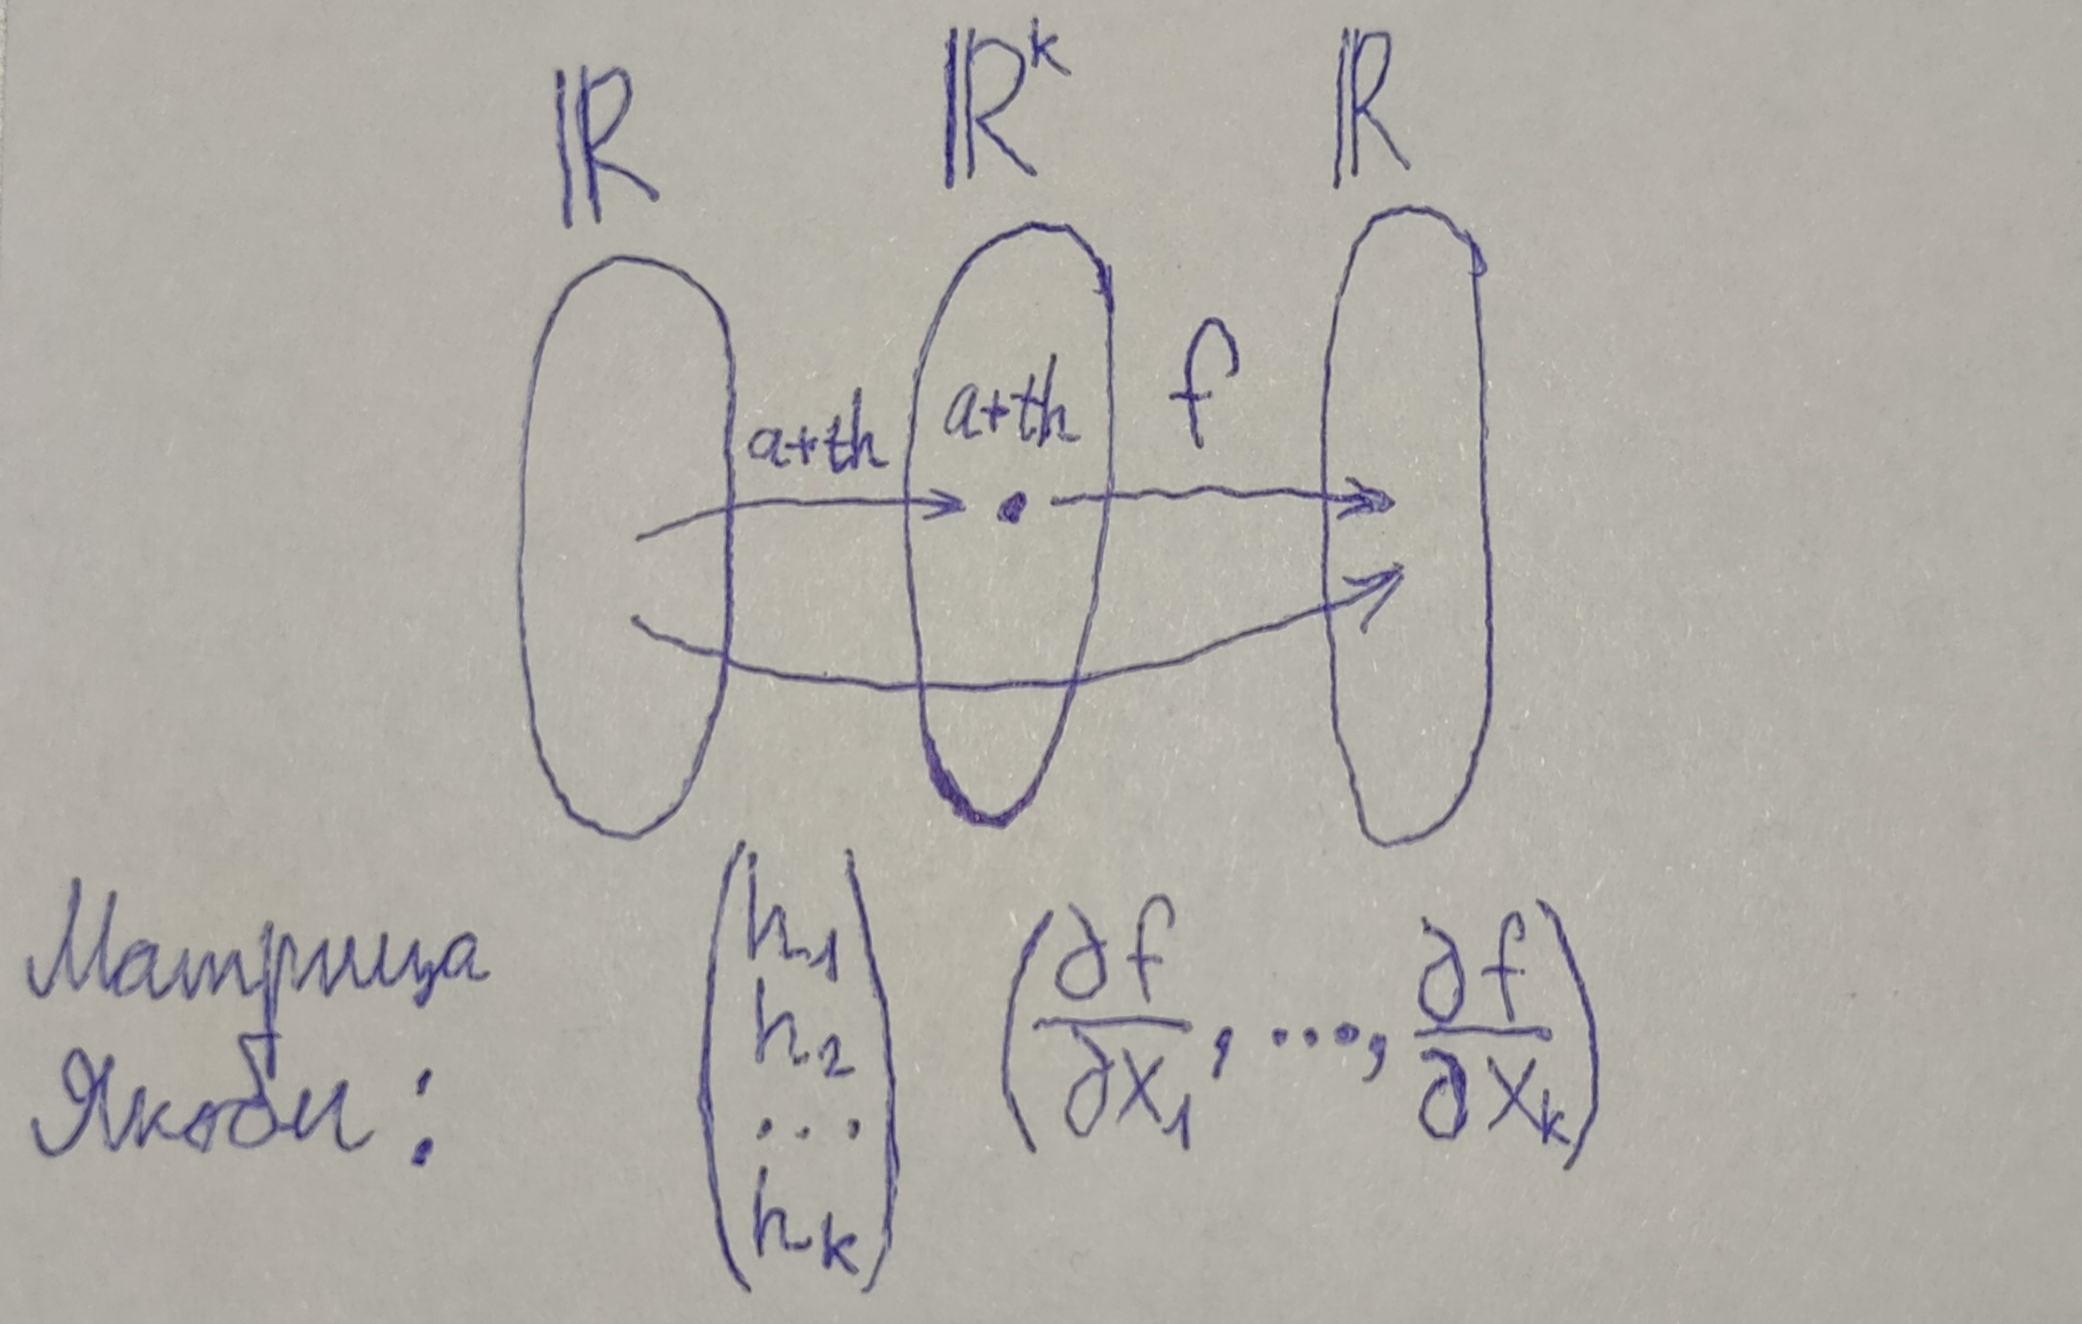
\includegraphics[width=0.4\textwidth]{img/lecture39/matrix_yakobi}
    	\end{center}    	
    	$\phi'(t) = f'(a + th) = \begin{pmatrix}
    		\deriv{f}{x_1} & \deriv{f}{x_2} & ... & \deriv{f}{x_k}
    	\end{pmatrix} \cdot \begin{pmatrix}
    	h_1 \\
    	h_2 \\
    	... \\
    	h_k
    	\end{pmatrix} = \deriv{f}{x_1}(a + th)h_1 + ... + \deriv{f}{x_k}(a + th)h_k = df\bigg|_{a + th}(h)$
    	
    	Переход:
    	\[ \phi^{(m + 1)}(t) = (\phi^{(m)}(t))' = (d^mf|_{a + th}(h))'_t = \bigg(\sum_{j_1, ..., j_m} \frac{\partial^m f(a + th)}{\partial x_{j_1} ... \partial x_{j_m}} h_{j_1} ... h_{j_m}\bigg)'_t = \]
    	\[ = \sum_{j_1, ..., j_m} \deriv{}{t} \bigg(\frac{\partial^m f(a + th)}{\partial x_{j_1} ... \partial x_{j_m}} h_{j_1} ... h_{j_m}\bigg) = \sum_{j_1, ..., j_m} \sum_{i = 1}^k \frac{\partial^{m + 1} f(a + th)}{\partial x_i \partial x_{j_1} ... \partial x_{j_m}} h_{j_1} ... h_{j_m} h_i = \]
    	\[ = \sum_{j_1, ..., j_{m + 1}} \frac{\partial^{m + 1} f(a + th)}{\partial x_{j_1} ... \partial x_{j_{m + 1}}} h_{j_1} ... h_{j_{m + 1}} = d^{m + 1}f|_{a + th}(h) \]
    \end{proof}
    
    \begin{theorem}
    	Пусть функция $f: \R^k \rightarrow \R$ $m$ раз непрерывно дифференцируема в окрестности точки $a$. Тогда справедлива следующая формула Тейлора:
    	\[ f(a + h) = f(a) + df|_a(h) + \frac{1}{2!}d^2 f|_a(h) + ... + \frac{1}{m!}df^{(m)}|_a(h) + o(||h||^m). \]
    \end{theorem}
    
    \begin{proof}
    	$\phi: \R \rightarrow \R, \phi(t) = f(a + th)$
    	\[ \phi(1) = \phi(0) + \phi'(0) \cdot 1 + ... + \frac{\phi^{(m - 1)}(0)}{(m - 1)!} + \frac{1}{(m - 1)!} \int_0^1 (1 - t)^{m - 1} \phi^{(m)}(t) \; dt = \]
    	\[ \text{(по лемме 15.3)} = f(a) + \frac{df|_a(h)}{1!} + ... + \frac{d^{m - 1}f|_a(h)}{(m - 1)!} + \frac{d^m f|_a(h)}{m!} + R_m \]
    	\[ R_m = \frac{1}{(m - 1)!} \int_0^1 (1 - t)^{m - 1} \phi^{(m)}(t) \; dt - \frac{\phi^{(m)}}{m!}(0) =  \frac{1}{(m - 1)!} \int_0^1 (1 - t)^{m - 1} \phi^{(m)}(t) \; dt - \]
    	\[ - \frac{1}{(m - 1)!} \int_0^1 (1 - t)^{m - 1} \phi^{(m)}(0) \; dt = \frac{1}{(m - 1)!} \int_0^1 (1 - t)^{m - 1}(\phi^{(m)}(t) - \phi^{(m)}(0)) \; dt \]
    	\[ \frac{|R_m|}{||h||^m} \leqslant \frac{\sup{|\phi^{(m)}(t) - \phi^{(m)}(0)|}}{||h||^m m!} =  \]
    	\[ = \sup{\bigg|\sum_{j_1, ..., j_m} \frac{\partial^m f(a + th)}{\partial x_{j_1} ... \partial x_{j_n}} h_1 ... h_m - \sum_{j_1, ..., j_m} \frac{\partial f(a)}{\partial x_{j_1} ... \partial x_{j_n}} h_1 ... h_m \bigg|} \frac{1}{||h||^m \cdot m!} = (*) \]
    	\[ \forall k \text{ } |h_{j_k}| \leqslant ||h|| \Rightarrow \frac{|h_{j_1} ... h_{j_m}|}{||h||^m} \frac{1}{m!} \leqslant \frac{1}{m!} \]
    	$m$-я производная функции непрерывна $\Rightarrow$
    	\[ \Rightarrow \sum_{j_1, ..., j_m} \frac{\partial^m f(a + th)}{\partial x_{j_1} ... \partial x_{j_n}} - \frac{\partial f(a)}{\partial x_{j_1} ... \partial x_{j_n}} \to 0 \text{ при } h \to 0 \]
    	Значит $(*) \to 0 \Rightarrow \frac{|R_m|}{||h||^m} \to 0 \Rightarrow R_m = o(||h||^m)$
    \end{proof}
    
    \section{Точка локального экстремума}
    
    \begin{definition}
    	Пусть функция $u = f(x), x \in \R^n$ определена в некоторой окрестности $U(x_0)$ точки $x_0$. Тогда $x_0$ называют точкой
    	\begin{itemize}
    		\item \underline{локального максимума} функции, если для всех точек $x \in U(x_0)$ верно неравенство $f(x) \leqslant f(x_0)$;
    		\item \underline{строгого локального максимума} функции, если для всех точек $x \in U(x_0)$ верно неравенство $f(x) < f(x_0)$;
    		\item \underline{локального минимума} функции, если для всех точек $x \in U(x_0)$ верно неравенство $f(x) \geqslant f(x_0)$;
    		\item \underline{строгого локального минимума} функции, если для всех точек $x \in U(x_0)$ верно неравенство $f(x) > f(x_0)$;
    		\item \underline{локального экстремума} функции, если она входит в одну из перечисленных выше категорий.
    	\end{itemize}
    \end{definition}
    
    \section{Необходимое условие локального экстремума}
    \begin{theorem}[Необходимое условие локального экстремума]
    	Пусть $a$ - точка локального экстремума функции $f$ и предположим, что $f$ дифференцируема в точке $a$. Тогда $df|_a = 0$ (или, что тоже самое, $\deriv{f}{x_j}(a) = 0$ $\forall j$).
    \end{theorem}
    
    \begin{proof}
    	Пусть $a$ - точка максимума $\Rightarrow$ при фиксированном $h$ и $t \neq 0$ $\phi(0) = f(a) > f(a + ht) = \phi(t)$.
    	
    	$\phi: \R \rightarrow \R \Rightarrow$ необходимое условие $\phi'(0) = 0 = df|_a(h)$ $\forall h$ по лемме 15.3 $\Rightarrow df|_a = 0$.
    \end{proof}
    
    \begin{definition}
    	Точки, в которых все частные производные равны нулю, называются \underline{стационарными}.
    \end{definition}
    
    \section{Достаточное условие локального экстремума}
    
    \begin{theorem}[Достаточное условие локального экстремума]
    	Пусть $f$ дважды непрерывно дифференцируема в окрестности точки $a$ и предположим, что в точке $a$ выполнено необходимое условие локального экстремума: $df|_a(h) = 0$ $\forall h$. Тогда
    	\begin{enumerate}
    		\item если $d^2f|_a(h) > 0$ $\forall h \neq 0$, то $a$ - точка строгого локального минимума;
    		\item если $d^2f|_a(h) < 0$ $\forall h \neq 0$, то $a$ - точка строгого локального максимума.
    	\end{enumerate}
    \end{theorem}
    
    \begin{proof}
    	Докажем первый пункт, второй доказывается аналогично. По теореме 15.4
    	\[ f(a + h) - f(a) = df|_a(h) + \frac{d^2f|_a}{2}(h) + o(||h||^2) = \frac{d^2f|_a}{2}(h) + o(||h||^2) = \]
    	\[ = ||h||^2 \bigg(\frac{d^2f|_a(\frac{h}{||h||})}{2} + o(1)\bigg) = (*) \]
    	$d^2f|_a(\frac{h}{||h||})$ - симметричная билинейная форма.
    	
    	Заметим, что квадратичная функция $d^2f\bigl|_a(q) = \sum_{i,j}\frac{\partial^2 f}{\partial x_i\partial x_j}(a)q_iq_j$ является симметричной квадратичной формой, и
    	как функция аргумента $q$ достигает свое минимальное значение на единичное сфере $\{h\colon \|q\|=1\}$. Действительно, симметричная квадратичная форма $B$ ортогональными преобразованиями $S$ приводится к диагональному виду $D$, поэтому
    	$$\min_{||u||=1} u^TBu = \min_{||u||=1} u^TS^TDSu = \min_{||v||=1} v^TDv = m,$$
    	где $m$ - минимальный элемент на диагонали матрицы $D$.
    	
    	Поэтому непрерывная функция $d^2f\bigl|_a(q)$ достигает на сфере
    	своего минимума:
    	\[ \min\limits_{||q|| = 1}d^2f\bigl|_a(q) = m=d^2f\bigl|_a(q_0) > 0. \]
    	Тогда
    	\[ (*) \geqslant ||h||^2 (\frac{m}{2} + o(1)) \Rightarrow \forall h \in B_{\delta}(a) \text{ } ||h||^2 (\frac{m}{2} + o(1)) \geqslant ||h||^2 \frac{m}{4} > 0. \]
    \end{proof}
    
    \section{Критерий Сильвестра}
   
    \begin{mention}
   	    Отметим, что $d^2f|_a(h)$ — это квадратичная форма
    	\[ \begin{pmatrix}
    		\frac{\partial^2 f}{\partial x_1^2}(a) & \frac{\partial^2 f}{\partial x_1 \partial x_2}(a) & ... & \frac{\partial^2 f}{\partial x_1 \partial x_k}(a) \\
    		\frac{\partial^2 f}{\partial x_1 \partial x_2}(a) & \frac{\partial^2 f}{\partial x_2^2}(a) & ... & \frac{\partial^2 f}{\partial x_2}{\partial x_k}(a) \\
    		... & ... & ... & ... \\
    	\end{pmatrix} \]
   	    Условие теоремы выше подразумевает её положительную или отрицательную определенность, что позволяет применить критерий Сильвестра:
   	    \begin{enumerate} 
   	    	\item все угловые миноры матрицы квадратичной формы $d^2 f|_a$ положительны $\Leftrightarrow d^2 f|_a$ - положительно определена (т.е. $d^2 f|_a(h) > 0$ при каждом $h \neq 0$);
   	    	\item угловые миноры матрицы квадратичной формы $d^2 f|_a$ начинаются с отрицательного, а затем чередуют знаки $\Leftrightarrow d^2 f|_a$ - отрицательно определена (т. е. $d^2 f|_a(h) < 0$ при каждом $h \neq 0$).
	    \end{enumerate}
    \end{mention}
    
    \section{Теорема о неявной функции}
    
    Для сокращения всех записей будем использовать обозначение $F'_y(x, y) := \deriv{F}{y}(x, y)$.
    
    \begin{theorem}
    	Пусть $F : \R^2 \rightarrow \R$ — определена и непрерывно дифференцируема (т. е. частные производные непрерывно зависят от точки) в некоторой окрестности $U$ точки $(a, b) \in \R^2$.
    	
    	Пусть $1)$ $F(a, b) = 0$ и $2)$ $F'_y(a, b) \neq 0$. Тогда найдутся промежутки $I_x = (a - \alpha, a + \alpha)$ и $I_y = (b - \beta, b + \beta)$ и непрерывно дифференцируемая функция $f : I_x \rightarrow I_y$, для которых $I_x \times Iy \subset U$ и для каждой точки $(x, y) \in I_x \times I_y$ выполнено $F(x, y) = 0 \Leftrightarrow y = f(x)$. Кроме того, $f'(x) = -\frac{F'_x(x, f(x))}{F'_y(x, f(x))}.$
    \end{theorem}
    
    \begin{proof}
    \end{proof}
    
    \begin{theorem}
    	Пусть $F : \R^{k + 1} \rightarrow \R$ - определена и непрерывно дифференцируема (т. е. частные производные непрерывно зависят от точки) в некоторой окрестности $U$ точки $(a, b) = (a_1, ..., a_k, b) \in \R^{k + 1}$. Пусть $1)$ $F(a, b) = 0$ и $2)$ $F'_y(a, b) \neq 0$. Тогда найдутся $I_x = (a_1 - \alpha_1, a_1 + \alpha_1) \times ... \times (a_k - \alpha_k, a_k + \alpha_k)$ и $I_y = (b - \beta, b + \beta)$ и непрерывно дифференцируемая функция $f : I_x \rightarrow I_y$, для которых $I_x \times I_y \subset U$ и для каждой точки $(x, y) \in I_x \times I_y$ выполнено $F(x, y) = 0 \Leftrightarrow y = f(x)$. Кроме того, $\deriv{f}{x_j}(x) = -\frac{F'_{x_j}(x, f(x))}{F'_y(x, f(x))}$.
    \end{theorem}
    
    \section{Теорема о неявном отображении}
    
    \begin{theorem}
    	Пусть отображение $F : \R^{k + n} \rightarrow \R^n$ — определено и непрерывно дифференцируемо в некоторой окрестности $U$ точки $(a, b) = (a_1, ..., a_k, b_1, ..., b_n) \in \R^{k + n}$. Пусть $1)$ $F(a, b) = 0$ и $2)$ матрица
    	\[ F'_y(a, b) := \begin{pmatrix}
    		\deriv{F_1}{y_1}(a, b) & ... & \deriv{F_1}{y_n}(a, b) \\
    		... & ... & ... \\
    		\deriv{F_n}{y_1}(a, b) & ... & \deriv{F_n}{y_n}(a, b) \\
    	\end{pmatrix} - \text{обратима.} \]
    	Тогда найдутся $I_x = (a_1 - \alpha_1, a_1 + \alpha_1) \times ... \times (a_k - \alpha_k, a_k + \alpha_k)$ и $I_y = (b_1 - \beta_1, b_1 + \beta_1) \times ... \times (b_n - \beta_n, b_n + \beta_n)$ и непрерывно дифференцируемое отображение $f = (f_1, ..., f_n): I_x \rightarrow I_y$, для которых $I_x \times I_y \subset U$ и для каждой точки $(x, y) \in I_x \times I_y$ выполнено
    	\[ F(x, y) = 0 \Leftrightarrow y = f(x). \]
    \end{theorem}

\end{document}
